\documentclass[
	11pt, % Default font size, select one of 10pt, 11pt or 12pt
	fleqn, % Left align equationsf
	a4paper, % Paper size, use either 'a4paper' for A4 size or 'letterpaper' for US letter size
	%oneside, % Uncomment for oneside mode, this doesn't start new chapters and parts on odd pages (adding an empty page if required), this mode is more suitable if the book is to be read on a screen instead of printed
]{LegrandOrangeBook}


\title{\Huge\textbf{A General Equation of Science}\\\Large\textbf{Implications}}
\AtBeginDocument{
  \hypersetup{
    pdftitle={A General Equation of Science. Implications},
    pdfauthor={Enrique Castillo Ron and Alfonso Fernández-Canteli},
    pdfsubject={Subject},
    pdfkeywords={Keyword1, Keyword2, ...},
  }
}
\usepackage{amsmath,amssymb}
\definecolor{ocre}{RGB}{243, 102, 25} % Define the color used for highlighting throughout the book
\chapterimage{orange1.jpg} % Chapter heading image
\chapterspaceabove{6.5cm} % Default whitespace from the top of the page to the chapter title on chapter pages
\chapterspacebelow{6.75cm} % Default amount of vertical whitespace from the top margin to the start of the text on chapter pages
\usepackage[utf8]{inputenc}
\usepackage[T1]{fontenc}
%----------------------------------------------------------------------------------------
% Otros paquetes matemáticos
\usepackage{bm}
\usepackage{centernot}
\usepackage{xkeyval}
\usepackage{placeins}
\usepackage{listings}
% Algorithm packages
\usepackage{algorithm}
%\usepackage{algorithmicx}
\usepackage{algpseudocode}
\usepackage{tikz}
\usetikzlibrary{shapes,arrows,positioning,calc}
% COMENTA natbib:
%\usepackage{natbib}
%\bibliographystyle{plainnat}
% USA biblatex que ya viene con la clase:
\addbibresource{bibliography.bib}
%C:\Users\Enrique\AppData\Local\Programs\MiKTeX\tex/latex/biblatex\biblatex
%\usepackage[backend=biber]{biblatex}
%\addbibresource{bibliography.bib}
%\usepackage[backend=biber,style=authoryear]{biblatex}
%\usepackage{tcolorbox}
% ===== REEMPLAZO DE TCOLORBOX POR MDFRAMED =====
% Reemplaza todo el código de tcolorbox por esto:
% Los paquetes ya están cargados en la clase
% \RequirePackage{mdframed}
% \RequirePackage{xcolor}
% Crear entorno problembox usando mdframed
\newmdenv[
    skipabove=7pt,
    skipbelow=7pt,
    backgroundcolor=blue!10,
    linecolor=blue!50,
    linewidth=1pt,
    roundcorner=3pt,
    innerleftmargin=8pt,
    innerrightmargin=8pt,
    innertopmargin=8pt,
    innerbottommargin=8pt,
    leftmargin=0cm,
    rightmargin=0cm
]{problembox}
% Comandos básicos de tcolorbox en caso de que aparezcan otros
\newcommand{\tcbset}[1]{}
\providecommand{\newtcolorbox}[3][]{%
    % Comando vacío para evitar errores si aparece en el código
}
% Crear entorno tcolorbox básico por si aparece en el documento
\newenvironment{tcolorbox}[1][]
{%
    \begin{mdframed}[
        backgroundcolor=gray!10,
        linecolor=gray,
        linewidth=1pt,
        roundcorner=3pt,
        skipabove=7pt,
        skipbelow=7pt,
        innerleftmargin=8pt,
        innerrightmargin=8pt,
        innertopmargin=8pt,
        innerbottommargin=8pt
    ]%
}
{%
    \end{mdframed}%
}
% ===== FIN DEL REEMPLAZO =====
% Custom mathematical commands
\newcommand{\R}{\mathbb{R}}
\newcommand{\N}{\mathbb{N}}
\newcommand{\Z}{\mathbb{Z}}
\newcommand{\Q}{\mathbb{Q}}
\newcommand{\C}{\mathbb{C}}
% Operadores matemáticos personalizados
\DeclareMathOperator{\rank}{rank}
\begin{document}
%\setkeys{Gin}{draft}

%----------------------------------------------------------------------------------------
%	TITLE PAGE
%----------------------------------------------------------------------------------------

\titlepage % Output the title page
	{\includegraphics[width=\paperwidth]{background.pdf}} % Code to output the background image, which should be the same dimensions as the paper to fill the page entirely; leave empty for no background image
	{ % Title(s) and author(s)
		\centering\sffamily % Font styling
		{\Huge\bfseries A General Equation of Science\par} % Book title
		\vspace{16pt} % Vertical whitespace
		{\LARGE Implications\par} % Subtitle
		\vspace{24pt} % Vertical whitespace
		{\huge\bfseries Enrique Castillo Ron\\ and\\ Alfonso Fernández-Canteli\par} % Author name
	}

%----------------------------------------------------------------------------------------
%	COPYRIGHT PAGE
%----------------------------------------------------------------------------------------

\thispagestyle{empty} % Suppress headers and footers on this page

~\vfill % Push the text down to the bottom of the page

\noindent Copyright \copyright\ 2025 Enrique Castillo Ron and Alfonso Fernández-Canteli\\ % Copyright notice

\noindent \textsc{Published by Publisher}\\ % Publisher

\noindent \textsc{\href{https://www.latextemplates.com/template/legrand-orange-book}{book-website.com}}\\ % URL

\noindent Licensed under the Creative Commons Attribution-NonCommercial 4.0 License (the ``License''). You may not use this file except in compliance with the License. You may obtain a copy of the License at \url{https://creativecommons.org/licenses/by-nc-sa/4.0}. Unless required by applicable law or agreed to in writing, software distributed under the License is distributed on an \textsc{``as is'' basis, without warranties or conditions of any kind}, either express or implied. See the License for the specific language governing permissions and limitations under the License.\\ % License information, replace this with your own license (if any)

\noindent \textit{First printing, March 2025} % Printing/edition date

%----------------------------------------------------------------------------------------
%	TABLE OF CONTENTS
%----------------------------------------------------------------------------------------

\pagestyle{empty} % Disable headers and footers for the following pages

\tableofcontents % Output the table of contents

\listoffigures % Output the list of figures, comment or remove this command if not required

\listoftables % Output the list of tables, comment or remove this command if not required

\pagestyle{fancy} % Enable default headers and footers again

\cleardoublepage % Start the following content on a new page


%\end{document}
%----------------------------------------------------------------------------------------
%	PART
%----------------------------------------------------------------------------------------
% PART I: WHAT IS THIS BOOK ABOUT?
\part{What is This Book About}

%----------------------------------------------------------------------------------------
%	SECTIONING EXAMPLES CHAPTER
%----------------------------------------------------------------------------------------

\chapterimage{orange2.jpg} % Chapter heading image
\chapterspaceabove{6.75cm} % Whitespace from the top of the page to the chapter title on chapter pages
\chapterspacebelow{7.25cm} % Amount of vertical whitespace from the top margin to the start of the text on chapter pages

%------------------------------------------------
\chapter[What can you expect from this book?]{What suggestive ideas and surprising results can you expect from this book?}\index{Sectioning}
\label{ch:whatthisbook}

\section{A Journey of Discovery: From  Particular to Universal Understanding}\index{Sectioning!Sections}
\begin{center}
\begin{minipage}{0.9\textwidth}
\setlength{\parskip}{2mm}
\setlength{\baselineskip}{1.1em}
{\it\footnotesize
"This book chronicles the research collaboration lived by the authors and their common experiences from the early 1980s to the present work. Beginning with statistical analysis of fatigue problems influenced by functional equations, we embarked on an expedition through the mountains of knowledge, driven by continual discoveries.

Our ascent began without a clear route and destination, obscured by clouds. We ventured into dense forests, investigating individual trees—roots, trunks, branches—becoming fascinated by details while seeking the broader perspective. Despite difficulties (exhaustion, doubts, confusion), we resisted becoming lost in specifics and eventually emerged from the forest.

When fog cleared, sunlight revealed both the summit and our path. Reaching the peak, we gained perspective not only on forests traversed and slopes climbed, but on other mountains and forests and their interconnected nature. This new perspective, achieved through understanding universal principles, leads us to believe that perhaps now is the time to return to examining those individual trees—their roots, trunks, branches, leaves, and fruits—but with the understanding that they represent something far more general shared across diverse disciplines.

The material that follows recounts this story, illustrated by those works of ours that marked significant milestones on our journey. What we began to discover in these works were the seeds that are now harvested in this present study, making it possible."}
\end{minipage}
\end{center}

%\cite{fourier1822}
%\bibliography{bibliography}

%\end{document}


Imagine discovering that the complexity of the natural world, from the flow of rivers to the behavior of financial markets, from quantum mechanical systems to the reliability of engineering structures, can be understood through a unified mathematical lens. This book unveils such a perspective, revealing how seemingly disparate phenomena share fundamental structural similarities that can be captured through elegant universal models.

At the heart of this exploration lies a profound question that has captivated scientists and engineers for centuries: Is it possible to develop a single, general-purpose mathematical framework that can model the vast diversity of multivariate functions encountered across scientific and engineering domains? These functions appear everywhere, in deterministic systems that follow precise physical laws, in stochastic processes governed by probability, in classical mechanics where Newton's equations reign supreme, and in the mysterious realm of quantum physics where uncertainty principles dominate.

The answer, as this book demonstrates, is a resounding yes. But the path to this answer reveals surprising insights that challenge conventional thinking about mathematical modeling, statistical analysis, and even the nature of information itself.

\section{The Quest for Universal Simplicity}\index{Sectioning!Sections}

Our journey begins with a deceptively simple goal: to develop models that are simultaneously maximally general and minimally complex. This might seem contradictory, how can something be both comprehensive and simple? The resolution of this apparent paradox leads us to one of the most elegant theorems in applied mathematics and engineering.

Chapter \ref{ch:historicalFoundations} provides a brief but essential foundation, tracing the intellectual lineage that makes our modern approach possible. We discover how the insights of mathematical giants like Fourier and Maxwell laid the groundwork for understanding that physical laws must be independent of the arbitrary units humans use to measure them. This seemingly obvious observation has profound implications that continue to reshape how we approach complex problems today.

The real adventure begins in Chapter \ref{ch:buckinghamPi} with the Buckingham Pi Theorem, a mathematical principle that acts as a powerful simplification engine. This theorem doesn't merely suggest using dimensionless variables; it guarantees that such simplifications are not only possible but necessary for any physically meaningful analysis. What makes this particularly surprising is that the theorem essentially tells us that nature "prefers" certain mathematical forms over others.

But here's where things get interesting: the Pi theorem, while guaranteeing the existence of simplified models, doesn't provide a unique solution. Chapter \ref{ch:Piforms} tackles this apparent limitation head-on, transforming what might seem like mathematical ambiguity into a powerful source of flexibility. We explore how to identify all possible dimensional ratios and maintain the freedom to choose among them, a capability that proves crucial for practical applications.

\section{The Revolutionary Power of Order}\index{Sectioning!Sections}

Perhaps the most surprising discovery presented in this book emerges from what initially appears to be a purely technical consideration. In Chapter \ref{ch:cdftransformation}, we introduce a universal transformation based on empirical distribution functions that maps all variables to the interval $[0,1]$. This transformation offers obvious practical advantages, numerical stability, enhanced comparability, mathematical convenience, universality and direct interpretability.

However, the deeper implications are startling: this transformation reveals that the actual values of variables matter far less than their relative ordering. This insight, that order, not magnitude, carries the essential information, represents a fundamental shift in how we think about data and mathematical relationships. Imagine realizing that whether you measure temperature in Celsius, Fahrenheit, or Kelvin matters less than understanding which measurements are higher or lower than others. This principle generalizes far beyond temperature to virtually any quantitative measurement.

This order-based perspective dramatically simplifies complex models without sacrificing their predictive power. It's as if we've discovered that nature communicates through rankings rather than absolute values, a truly remarkable result with implications that extend far beyond mathematical modeling.

\section{Networks That Learn Functions, Not Just Weights}\index{Sectioning!Sections}

The mathematical structures that emerge from our analysis in Chapter \ref{ch:Piforms} reveal something unexpected: they naturally organize themselves into network-like architectures. But these aren't conventional neural networks. Instead of learning connection weights while keeping activation functions fixed, our "functional networks" learn the activation functions themselves, connecting them through associative operations.

This reversal of the traditional neural network paradigm opens entirely new possibilities. Rather than hoping that fixed mathematical functions (like sigmoids or ReLUs) can approximate any relationship through weight adjustment, we allow the functions themselves to evolve and adapt to the data. The resulting models in Chapter \ref{ch:resultingmodel} are both more interpretable and more powerful than their traditional counterparts.

The iterative aggregation of variables in these networks yields another surprising property: it doesn't matter whether you combine variables individually or in groups, the final result remains equivalent. This mathematical robustness provides both theoretical elegance and practical flexibility.

\section{From Deterministic Laws to Probabilistic Reality}

The versatility of our framework becomes apparent through carefully chosen examples that span the spectrum from classical deterministic applications to cutting-edge stochastic modeling. Chapter \ref{ch:firstexampleACtion-Interactions} demonstrates how the Pi Theorem's classical applications, dimensional analysis for laboratory scaling and formula simplification, fit naturally within our broader framework. We examine conditional distribution CDFs, ubiquitous in most engineering applications, showing how our approach handles real-world complexity.

But the second example marks a conceptual leap that many readers will find both surprising and illuminating. Chapter \ref{ch:copulas} shifts the entire framework into the realm of probability, treating our multivariate function as a joint cumulative distribution function of random variables. This isn't merely an academic exercise, it reflects a profound truth about the world around us.

Real-world problems are inherently probabilistic, not deterministic. Even when we write down deterministic equations, uncertainty in measurements, environmental conditions, and model parameters means that probabilistic thinking is more realistic from the outset. Our learning databases are populations whose selection criteria is, unfortunately, commonly unknown and this implies randomness.  Our framework bridges deterministic and stochastic models, revealing them as different aspects of the same underlying mathematical structure.

This probabilistic perspective leads us naturally to statistical copulas, mathematical objects that permit separating the individual behavior of variables from their joint dependencies. Copulas allow us to disentangle what each variable contributes individually from how variables interact collectively. More remarkably, they enable the reconstruction of multivariate random systems that differ only in their marginal transformations while sharing identical dependency structures.

\section{The Emergence of Universal Probability Models}\index{Sectioning!Sections}

Chapter \ref{ch:copulaapplication} reveals a striking result: when we apply our general model to find compatible copulas, only Archimedean copulas satisfy the structural requirements. This isn't merely a mathematical curiosity, it suggests that certain probabilistic relationships are more "natural" or fundamental than others, appearing automatically when we impose reasonable structural constraints.

The story takes another unexpected turn in Chapter \ref{ch:bayesian} with the introduction of Bayesian networks as the missing piece of our probabilistic puzzle. While copulas excel at capturing marginal influences, Bayesian networks complete the picture by handling conditional dependencies among variable subsets. This combination leads to a remarkable conclusion: the optimal copula structure turns out to be the product copula, which allows us to learn each variable independently.

However, these variables are now conditional random variables, not simple independent ones. This subtle but crucial distinction leads to what can legitimately be called a universal model for multivariate random variables. The implications are profound: complex probabilistic systems can be decomposed into simpler, more manageable components without losing essential information about their joint behavior, and the learning process of thes variables can be done one by one.

What copulas accomplish for marginal distributions, Bayesian networks achieve for arbitrary variable subsets. This symmetry and completeness provide both theoretical satisfaction and practical power.

\section{Structure-Driven Network Architecture}\index{Sectioning!Sections}

Perhaps most surprisingly, the Bayesian network structure that emerges from our probabilistic analysis provides the reference framework for our functional networks. Chapter \ref{ch:newfunctionalnetworks} demonstrates that network architecture need not be arbitrary or based solely on empirical performance. Instead, mathematical and statistical principles can guide the construction of network structures that are both well-founded and effective.

Since the Pi theorem enables complexity reduction through dimensional analysis, our networks naturally organize themselves into stages. The first stage identifies dimensionless ratios—not just a single particular choice, but the complete set of possible combinations. This comprehensive approach ensures that the learning process can explore all reasonable options without being constrained to predetermined selections.

The subsequent stages implement CDF transformations and incorporate Bayesian network principles, creating an architecture that is both rigorously grounded and adaptable. The resulting functional networks represent a new paradigm that combines the strengths of traditional neural networks with the theoretical rigor of dimensional analysis and probabilistic modeling.

\section{Practical Applications and Visualization Tools}\index{Sectioning!Sections}

The theoretical developments find concrete expression in Chapter \ref{ch:newaitool}, which leverages Bayesian network structures to create practical applications for multivariate data analysis. The chapter presents an innovative web-based tool that allows users to visualize complex multivariate relationships and easily obtain conditional and marginal distributions, making an intelligent use of Bayesian networks independence properties.

This application demonstrates that our theoretical framework translates into practical tools that can handle real-world data analysis challenges. The ability to visualize multivariate dependencies and extract conditional information represents a significant advance in making complex statistical concepts accessible to practitioners across diverse fields.

\section{Toward Universal Understanding}\index{Sectioning!Sections}

Chapter \ref{ch:conclusions} synthesizes these discoveries and points toward future research directions motivated by the material presented throughout the book. The quest for universal mathematical formulations to describe physical and engineering phenomena represents one of science's most enduring aspirations.

The concept of representing any physical or engineering problem through a universal equation of the form $\phi(\pi_1, \pi_2, \dots, \pi_n) = 0$, where $\pi_i$ represent dimensionless parameters, embodies the culmination of this centuries-long endeavor. This book demonstrates that such universality is not merely an abstract ideal but an achievable reality with concrete applications and profound implications.

\section{What Makes This Journey Surprising}\index{Sectioning!Sections}

Readers can expect several genuinely surprising discoveries that challenge conventional wisdom:

\textbf{The Primacy of Order Over Magnitude}: The revelation that relative ordering contains more essential information than absolute values overturns traditional thinking about data analysis and mathematical modeling.

\textbf{Function Learning Over Weight Learning}: The demonstration that learning functions rather than weights can produce more powerful and interpretable models challenges the entire neural network paradigm.

\textbf{Probabilistic Unity}: The discovery that deterministic and stochastic models are different manifestations of the same underlying mathematical structure provides a unifying perspective that has been missing from the literature.

\textbf{Natural Mathematical Structures}: The finding that certain mathematical forms (like Archimedean copulas) emerge naturally from structural constraints suggests that mathematics reflects deep truths about the organization of information and relationships.

\textbf{Universal Decomposition}: The demonstration that complex multivariate systems can be decomposed into simpler components without information loss provides both theoretical insight and practical computational advantages.

\textbf{Bayesian Networks}: The fact that Bayesian networks extend the representation properties of copulas in the sense that not only the effects of unidimensional marginals but multivariate marginals can be separated from the interaction effects of the remaining variables surprises and shows their potential power and probabilistic relevance.

\textbf{Multivariate representations of data and variables}: They allow to visualize multivariate interactions and provide extremely valid graphic inference information.

\textbf{Sensitivity analysis be made in real time}: All these tools reveal how sensitivity analysis can be made in real time.

These discoveries combine to form a coherent framework that is simultaneously practical and profound, offering new tools for analysis while revealing fundamental principles about the mathematical structure of reality itself. The journey through this book will change how readers think about modeling, probability, networks, and the deep connections between mathematics and the natural world.

The adventure begins with historical foundations and culminates in universal principles, but the path between reveals surprises that will reshape your understanding of mathematical modeling and its applications across science and engineering.



% PART II: THEORETICAL FOUNDATIONS
\part{Historical Foundations}

\chapter{Historical Foundations and Universal Modeling}
\label{ch:historicalFoundations}
\section{Historical Foundations}\index{Sectioning!Sections}

The development of dimensional analysis and universal modeling represents one of the most profound intellectual achievements in the physical sciences, fundamentally changing how we understand the relationship between mathematical descriptions and physical reality. This transformation began with the recognition that the laws of nature must possess an intrinsic independence from the arbitrary units humans use to measure physical quantities, a principle that has evolved into sophisticated methodologies for creating universal equations applicable across diverse phenomena and scales.

\subsection{Early Contributions and Fourier's Legacy}\index{Sectioning!Subsections}

The conceptual foundation of dimensional analysis can be traced directly to the pioneering work of Joseph Fourier in his seminal 1822 treatise on heat conduction \cite{fourier1822}. Fourier's contribution extended far beyond the specific mathematical treatment of thermal phenomena; he articulated for the first time the fundamental principle that physical laws must remain invariant under changes in the units of measurement. This insight emerged from his careful analysis of heat conduction equations, where he observed that the mathematical relationships describing temperature distribution and heat flow maintained their essential character regardless of whether temperatures were measured in degrees Celsius or Fahrenheit, or whether distances were expressed in meters or feet.

The profound implications of Fourier's principle become apparent when we consider that it establishes a bridge between the abstract mathematical formulation of physical laws and their concrete manifestation in the natural world. When Fourier demonstrated that an equation such as $F = ma$ must retain its validity whether force is measured in Newtons or pounds, mass in kilograms or slugs, and acceleration in meters per second squared or feet per second squared, he was essentially arguing that physical laws possess an objective reality that transcends human conventions of measurement.

This foundational insight was further developed and systematized by James Clerk Maxwell \cite{maxwell1873}, whose contributions to dimensional analysis paralleled his revolutionary work in electromagnetic theory. Working in collaboration with Fleeming Jenkin, Maxwell established the modern framework for understanding dimensional relationships by clearly distinguishing between fundamental and derived quantities. Maxwell's approach was methodical and comprehensive: he identified mass, length, and time as what he termed "the three fundamental units," while demonstrating that all other physical quantities could be expressed as combinations of these basic dimensions.

Maxwell's work was particularly significant because it provided both theoretical justification and practical methodology for dimensional analysis. He showed, for instance, that gravitational mass could be derived from length and time by invoking Newton's law of universal gravitation, thereby reducing the number of truly independent dimensions required to describe mechanical phenomena. This reduction principle would later become central to the systematic approaches developed in the twentieth century.

\subsection{Development of Systematic Approaches}\index{Sectioning!Subsections}

The transition from Fourier and Maxwell's foundational insights to practical analytical methods occurred primarily in the early decades of the twentieth century, driven by the increasing complexity of engineering problems and the need for systematic approaches to experimental design and data interpretation.

\subsubsection{Lord Rayleigh's Pioneering Method}

Lord Rayleigh, working under his given name J.W. Strutt, developed what became known as the Rayleigh method in the early 1900s \cite{rayleigh1915}. This represented the first systematic attempt to create a general procedure for dimensional analysis that could be applied consistently across different physical problems. Rayleigh's approach was based on the assumption that functional relationships between physical variables could be expressed in terms of power-law combinations, leading to equations of the form:

\begin{equation}
D = C \cdot l^a \cdot \rho^b \cdot \mu^c \cdot V^d \cdot g^e
\end{equation}
where $D$ represents the dependent variable of interest, $C$ is a dimensionless constant, and the exponents $a$, $b$, $c$, $d$, and $e$ are determined by requiring dimensional consistency across the equation.

For those who become surprised because of the presence of the $C$ constant, I give the example of the area of a rectangle, which is $A=C\cdot b \cdot h$, with $A$ its area and $b,h$ its basis and height, respectively. Since all of then can be measured in different units of magnitude, we need the constant $C$ for adjustment. When $C=1$, we can say that the units are coherent and then, the common formula 'basis times height' arises, but only then.

The Rayleigh method represented a significant advance because it provided a systematic procedure that could be taught and applied by engineers and scientists working on practical problems. The method involves several distinct steps: first, identifying all the physical variables that might influence the phenomenon under study; second, expressing the assumed functional relationship in power-law form; third, writing out the dimensional equation by replacing each variable with its dimensional formula; and finally, solving the resulting system of algebraic equations to determine the unknown exponents.

Despite its systematic nature, the Rayleigh method possessed inherent limitations that became increasingly apparent as it was applied to more complex problems. The assumption of power-law relationships, while mathematically convenient, proved restrictive when dealing with phenomena involving exponential, logarithmic, or other non-algebraic dependencies. Additionally, as the number of variables increased, the method became algebraically cumbersome and increasingly prone to computational errors.

\subsubsection{Buckingham's Systematic Framework}

The next major advancement came with Edgar Buckingham's comprehensive treatment of dimensional analysis in his influential 1914 paper \cite{buckingham1914}. Buckingham's work emerged from his investigation of the "screw propeller" problem, a practical engineering challenge that had significant implications for naval architecture and early aviation. Through his analysis of this problem, Buckingham recognized that dimensional analysis represented far more than a mathematical curiosity; it was, in his words, "a powerful tool for scaling measurements made on models and relating them to full scale."

Buckingham's insight was particularly prescient given the historical context. Writing in 1914, he observed that "This subject seems to be less familiar to physicists than it deserves to be," a comment that reflects the fact that dimensional analysis had not yet achieved widespread recognition within the scientific community. However, Buckingham understood that the principles he was developing would eventually become fundamental to engineering practice, particularly in the design and interpretation of laboratory experiments using scaled models.

The significance of Buckingham's contribution lies not only in his theoretical developments but also in his recognition of the practical importance of similarity and scaling relationships. He understood that the ability to relate measurements made on small-scale laboratory models to the behavior of full-scale systems would become increasingly important as engineering systems grew in size and complexity. This insight proved remarkably accurate, as dimensional analysis and similarity theory now underpin virtually all experimental work in fluid mechanics, structural engineering, and many other fields.

\section{Theoretical Frameworks for Universal Modeling}\index{Sectioning!Sections}

The evolution from early dimensional analysis methods to comprehensive theoretical frameworks for universal modeling represents a fundamental shift in scientific thinking about the nature of physical laws and their mathematical representation. This transformation reflects a growing understanding that the most powerful scientific theories are those that can describe diverse phenomena through unified mathematical structures.

\subsection{Similarity Theory and Physical Modeling}\index{Sectioning!Subsections}

The concept of similarity provides the theoretical foundation for universal modeling approaches. At its core, similarity theory addresses the fundamental question of when two apparently different physical situations can be considered equivalent from a scientific perspective. The formal definition of similarity states that two physical phenomena are similar when the numerical values characterizing one phenomenon can be used to derive the corresponding values for the other through a simple mathematical transformation analogous to converting between different systems of units.

This definition, while seemingly straightforward, has profound implications for both theoretical understanding and practical applications. It suggests that the essential physics of phenomena can be captured through appropriate dimensionless combinations of the relevant variables, and that these dimensionless groups provide the key to understanding when different systems will exhibit similar behavior.

The mathematical foundation of similarity theory rests on the principle that for any set of similar phenomena, all corresponding dimensionless characteristics must have identical numerical values. This principle can be stated as both a necessary and sufficient condition: if two phenomena are similar, their dimensionless parameters will be equal; conversely, if all relevant dimensionless parameters are equal for two phenomena, then these phenomena must be physically similar.

The power of this approach becomes evident when we consider its implications for experimental design and data interpretation. Rather than requiring separate investigations of every possible combination of system parameters, similarity theory allows researchers to identify the critical dimensionless groups that govern system behavior and then design experiments that systematically vary these groups while maintaining similarity conditions.

\subsubsection{Scale Invariance and Universal Applications}

The principle of scale invariance represents one of the most elegant and practically important consequences of similarity theory. Scale invariance implies that the fundamental relationships governing physical phenomena remain unchanged as we move from laboratory-scale investigations to full-scale applications, provided that the appropriate dimensionless parameters are maintained constant.

This principle has found extensive application across the engineering and physical sciences \cite{zierep1991}. In fluid mechanics, for example, scale invariance allows engineers to study the flow around aircraft models in wind tunnels and confidently extrapolate their results to full-scale aircraft, provided that key dimensionless parameters such as Reynolds number and Mach number are appropriately matched or accounted for.

The importance of scale invariance extends beyond its practical applications to experimental design. It provides fundamental insights into the nature of physical laws themselves, suggesting that the most fundamental descriptions of natural phenomena should be expressible in terms of dimensionless relationships that remain valid across all relevant scales. This insight has guided the development of universal modeling approaches that seek to identify these fundamental dimensionless relationships and express them in mathematical forms that can be applied across diverse physical situations.

\subsection{Dimensional Analysis as a Universal Tool}\index{Sectioning!Subsections}

Dimensional analysis has evolved from its origins as a specialized mathematical technique into a universal tool for understanding and predicting physical phenomena. The modern conception of dimensional analysis extends far beyond the mechanical application of dimensional consistency requirements to encompass a comprehensive methodology for extracting maximum information from limited knowledge about physical systems.

The fundamental premise underlying dimensional analysis is that any physical phenomenon can be described by a dimensionally consistent equation constructed from the physical parameters that influence the phenomenon. This premise, while simple in statement, has far-reaching implications for how we approach the investigation of complex physical systems. It suggests that even when we lack detailed theoretical understanding of the mechanisms governing system behavior, we can still derive significant insights by carefully identifying the relevant physical parameters and constructing appropriate dimensionless combinations.

The methodology of dimensional analysis provides several distinct advantages in the investigation of physical phenomena. First, it offers a systematic approach to problem simplification by reducing the number of independent variables that must be considered. Rather than investigating the separate effects of each individual parameter, dimensional analysis allows us to identify the fundamental dimensionless groups that govern system behavior, thereby reducing both the complexity of theoretical analysis and the scope of required experimental investigation.

Second, dimensional analysis provides a framework for establishing dimensionless numbers that serve as convenient figures of merit for comparing the characteristics of different systems. These dimensionless numbers often have clear physical interpretations that provide insight into the underlying physics of the phenomena being studied. The Reynolds number, for example, represents the ratio of inertial to viscous forces in fluid flow, while the Froude number characterizes the relative importance of inertial and gravitational effects.

Third, dimensional analysis offers universal applicability based on the concept of similarity. This universality implies that the insights gained from dimensional analysis of one particular system can often be extended to other systems that involve similar physical processes, even when the specific details of these systems differ significantly.

\section{Methodological Approaches}\index{Sectioning!Sections}

The development of systematic methodologies for dimensional analysis and universal modeling has proceeded through several distinct phases, each characterized by increasingly sophisticated mathematical techniques and broader conceptual frameworks. Understanding this evolution provides important insight into both the capabilities and limitations of different approaches.

\subsection{Beyond the Rayleigh Method}\index{Sectioning!Subsections}

While the Rayleigh method provided the first systematic approach to dimensional analysis, subsequent developments have addressed many of its limitations while extending the scope of dimensional analysis to increasingly complex problems. These advanced approaches can be broadly categorized into three main methodological frameworks, each with distinct advantages and areas of application.

The equation analysis method represents perhaps the most rigorous approach to similarity and dimensional analysis. This method begins with the fundamental differential equations that govern the physical phenomenon under investigation and derives similarity parameters directly from these equations through systematic mathematical analysis. The advantage of this approach is that it ensures that all relevant physical processes are properly accounted for in the final similarity relationships. However, the method requires detailed knowledge of the governing equations, which may not always be available for complex systems or poorly understood phenomena.

Integral, which use integrals as its main tool, differential, based on derivatives of one or several orders, and functional equations, expressed in terms of functions defined at different points in a domain, permit identifying important universal equations, that reflect related properties. They constitute a very elegant way of obtaining the initially unknown structure of physical and engineering equations. Their unique structures  allow us to separate models into two complementary groups, those that satisfy the property but also, the not less important group, of those that do not satisfy it. This suggests that models can be derived based on common sense or strongly accepted related properties, as a suggestive alternative to models based on more or less arbitrary or convenience assumptions. Equilibrium, static or dynamic, and balance equations are the most common used principles to derive these equations.

Since integral and differential equations are better known that functional equations, we provide a simple but illustrative example of the last ones. Consider one is interested in finding a model to obtain the damage, $d$, of an element having initially $d_0$ damage $t$ days later, that is, the aim is a formula, $d=f(d_0,t)$. Then, we can consider the following property, written as the functional equation
$$
f(d_0, t_1+t_2)=f(f(d_0, t_1), t_2)
$$
with unknown function $f()$. This property expresses that the same final damage $d$ is obtained if one starts at damage $d_0$ and uses it for $t_1+t_2$ days than if one uses it first for $t_1$ days and considers the resulting damage as the initial damage for a second period of $t_2$ days.  It can be shown that the general solution of this functional equation is:
$$
f(d_0, t) = \phi(\phi^{-1}(d_0)+t),
$$
where $\phi()$ is a univariate invertible function.

The property that we have used is so strong that the initial problem of identifying a bivariate function simplifies to obtaining an invertible univariate function, and, in addition, with the indicated structure. Those functions not of this form do not satisfy the property and lead to seriuos problems when used if the property is inexcusable in our model.

One surprising result for those not familiar with functional equations is that we can have arbitrary functions in the solution, not only constant parameters, as our degrees of freedom. In addition, as we shall see in this book, one single equation can involved several unknown functions, whose structures can be found. In other words, we do not need as many equations as unknowns to solve them.


Returning to our initial discussion, the law analysis method takes a somewhat different approach by deriving similarity parameters from well-established physical laws and conservation principles rather than from specific differential equations. This method is particularly valuable when dealing with systems where multiple physical processes interact in complex ways, making it difficult to write down complete governing equations. By focusing on fundamental conservation laws such as conservation of mass, momentum, and energy, the law analysis method can often identify the most important similarity parameters even for complex systems.

The dimensional analysis method, in its modern form, employs sophisticated mathematical techniques from linear algebra to systematically identify all possible dimensionless combinations of the relevant physical parameters. This approach uses matrix methods to determine the complete set of dimensionally independent groups, ensuring that no important dimensionless parameters are overlooked. The method is particularly valuable for complex systems involving large numbers of variables, where traditional approaches might miss important parameter combinations.

\subsection{Modern Computational Integration}\index{Sectioning!Subsections}

The integration of computational methods with traditional dimensional analysis represents one of the most significant recent developments in the field. This integration has been facilitated by advances in both computational hardware and software, but more fundamentally by changing perspectives on the nature of scientific modeling itself.

The contribution of cybernetics to scientific modeling \cite{longo2021} has been particularly significant in this context. Cybernetics, understood as the theory of models in science, has introduced new ways of thinking about the relationships between physical systems, mathematical models, and computational implementations. Rather than viewing these as separate and distinct entities, cybernetics encourages a more integrated perspective that recognizes the fundamental interconnections between physical phenomena, mathematical description, and computational analysis.

This cybernetic perspective has important implications for dimensional analysis and universal modeling. It suggests that the boundaries between different scientific disciplines are often artificial constructs that can limit our understanding of complex systems. By adopting a cybernetic approach that transcends traditional disciplinary boundaries, researchers can develop more comprehensive and powerful modeling frameworks that integrate insights from physics, biology, economics, and other fields.

Modern computational approaches to dimensional analysis typically combine traditional dimensional analysis techniques with advanced numerical methods. Computational fluid dynamics provides the capability to solve complex flow problems that would be impossible to address through analytical methods alone, while still respecting the dimensional relationships identified through classical analysis. Finite element analysis enables the investigation of structural and mechanical systems with complex geometries and material properties, again within the framework established by dimensional analysis.

Perhaps most significantly, machine learning techniques are beginning to be applied to the problem of identifying optimal functional forms for universal equations. Rather than relying on theoretical insight or experimental trial and error to determine the specific mathematical relationships between dimensionless parameters, machine learning algorithms can systematically search through large spaces of possible functional forms to identify those that best fit experimental or computational data.

\section{Engineering and Scientific Applications}\index{Sectioning!Sections}

The practical applications of dimensional analysis and universal modeling span virtually every area of engineering and applied science. These applications demonstrate both the power and the limitations of dimensional approaches, while illustrating how theoretical insights translate into practical engineering solutions.

\subsection{Fluid Mechanics}\index{Sectioning!Subsections}

Fluid mechanics provides perhaps the most extensive and well-developed applications of dimensional analysis and similarity theory. The field offers numerous examples of how dimensional analysis can simplify complex problems and provide insights that would be difficult to obtain through other approaches.

Consider the practical problem facing a hydraulic engineer who needs to determine how varying the diameter of a pipe affects the flow rate of fluid through the system. This problem involves several physical parameters: the pipe diameter, the density and viscosity of the fluid, the pressure difference driving the flow, and potentially gravitational effects if the pipe is not horizontal. Without dimensional analysis, investigating this problem would require extensive experimental work exploring the separate effects of each parameter.

Dimensional analysis transforms this complex multi-parameter problem into a much simpler investigation involving a smaller number of dimensionless groups. The analysis typically yields seven fundamental dimensionless parameters, including the drag coefficient, Reynolds number, Froude number, and several others that are cornerstone parameters in fluid mechanics analysis. These dimensionless parameters each have clear physical interpretations: the Reynolds number characterizes the relative importance of inertial and viscous effects, the Froude number represents the ratio of inertial to gravitational forces, and so forth.

The power of this dimensional approach becomes evident when we recognize that experimental investigations need only explore the behavior of these dimensionless parameters rather than each individual physical variable. This dramatically reduces the scope of required experimental work while providing results that can be applied to a wide range of different systems with different physical dimensions, fluid properties, and operating conditions.

\subsection{Materials and Structural Engineering}\index{Sectioning!Subsections}

The application of dimensional analysis to materials science and structural engineering presents both opportunities and challenges that differ from those encountered in fluid mechanics. Materials behavior often involves complex relationships between stress, strain, temperature, time, and microstructural parameters that cannot always be captured through simple dimensional relationships.

Physical modeling for metal plastic forming processes exemplifies both the potential and the limitations of dimensional approaches in materials science. As described by Liu and colleagues \cite{liu2000}, physical modeling in this context can be defined as "a research method on metal plastic forming processes by substituting the prototype for a model which can represent the important characteristics of the prototype and has the same physical nature as the prototype."

The challenge in applying similarity theory to metal forming processes lies in ensuring that all relevant physical mechanisms are properly scaled between the model and prototype systems. Unlike fluid mechanics problems, where the governing equations are well established and the relevant dimensionless parameters are well understood, metal forming involves complex interactions between mechanical deformation, heat transfer, microstructural evolution, and other phenomena that may not scale in simple ways.

Similarity theorem requires that all influential similarity parameters remain equal under geometric similarity conditions. However, achieving this requirement in practice often proves impossible because different physical processes may require conflicting scaling relationships. For example, maintaining geometric similarity may require one scaling relationship, while maintaining thermal similarity may require a different and incompatible relationship.

\subsection{Aerospace Applications}\index{Sectioning!Subsections}

Aerospace engineering has been one of the most successful areas for the application of dimensional analysis and similarity theory, largely because the fundamental physics of fluid flow around aircraft and spacecraft is well understood and can be described through established governing equations.

The use of dimensional analysis in aerospace applications typically focuses on establishing dimensionless numbers for comparing aircraft of varying sizes and flight conditions. The coefficient of lift, Reynolds number, Froude number, and Strouhal number serve as commonly used dimensionless parameters that characterize different aspects of aircraft performance. Each of these parameters captures important physical effects: the lift coefficient characterizes the aerodynamic efficiency of the aircraft configuration, the Reynolds number indicates whether the flow will be laminar or turbulent, and the Mach number determines the importance of compressibility effects.

The development of similarity relations for flight control systems represents a more recent and sophisticated application of dimensional analysis to aerospace problems. Modern aircraft employ complex feedback control systems that must maintain stable and responsive flight characteristics across a wide range of flight conditions. Dimensional analysis provides a framework for scaling control system parameters between different aircraft sizes and flight regimes, ensuring that control system performance remains consistent as aircraft configurations and operating conditions change.

\section{Contemporary Developments}\index{Sectioning!Sections}

The field of dimensional analysis and universal modeling continues to evolve rapidly, driven by advances in computational capabilities, new theoretical insights, and the increasing complexity of engineering systems. Contemporary developments focus primarily on extending traditional dimensional analysis methods to more complex systems and integrating these methods with modern computational and analytical techniques.

\subsection{Generalized Universal Frameworks}\index{Sectioning!Subsections}

Modern approaches to dimensional analysis emphasize the development of generalized frameworks that can accommodate the complexity and multi-physics nature of contemporary engineering systems. These frameworks recognize that many important engineering problems cannot be adequately addressed through traditional single-physics approaches, but require integrated treatment of coupled phenomena involving fluid flow, heat transfer, chemical reactions, electromagnetic effects, and other physical processes.

The development of universal equations of the form $\phi(\pi_1, \pi_2, \dots, \pi_n) = 0$ represents the ultimate extension of dimensional analysis principles. These equations embody the insight that complex physical phenomena can often be described through relationships between appropriately chosen dimensionless parameters, where the specific functional form of the relationship $\phi$ must be determined through theoretical analysis, experimental investigation, or computational methods.

The challenge in developing such universal equations lies in identifying the complete set of relevant dimensionless parameters $\pi_i$ and determining the appropriate functional relationship $\phi$. The first challenge requires comprehensive understanding of all the physical processes that influence system behavior, while the second requires sophisticated mathematical and computational techniques for functional form identification.

In fact, The same mathematical equation can represent several different mathematical, economics, physical or engineering problems. For example, the system of functional equations:
$$
f(x,y_1+y_2) = f(x, y_1) + f(x, y_2); \quad f(x_1 + x_2, y) = f(x_1, y) + f(x_2, y),
$$
where $A=f(x, y)$ could represent the area of a rectangle with basis $x$ and height $y$, but also the amount of money, $A$, received after depositing an amount of money $x$ during a time $y$ in a bank under simple interest. This relation expresses that the area of a rectangle with basis x and height $y_1+y_2$ is equal to the sum of the area of a rectangle of basis $x$ and height $y_1$ and the area of another rectangle of basis $x$ and height $y_2$ and that the area of a rectangle with basis $x_1 + x_2$ and height $y$ is equal to the sum of the area of a rectangle with basis $x_1$ and height $y$ and the area of another rectangle with basis $x_2$ and height $y$, in the case of a rectangle, and that the amount of money received after a period of time $y$ when depositing the amount $x$ is independent of how we divide the amount of money, $x$, and the time, $t$, in parts. We note that the solution of the system is:
$$
A = C X t,
$$
where $C$ is a constant, which for the interest problem is the interest rate. In the case of the rectangle, the $C$ is required when we use non-coherent units for measuring the basis, the height and the area. The common rule "the area of a rectangle is its basis times its height" does not become valid if non-coherent units are selected, and then $c$ comes as a necessary term to correct for this unit coherence. Surprising and unexpected warning message, given by functional equations, about the lack of generality of the common formula for the area of a rectangle.

Finally, recent advances in this area have focused on developing systematic procedures for parameter identification and functional form determination. These procedures often combine traditional dimensional analysis with advanced mathematical techniques such as group theory, differential geometry, and information theory to ensure that no important parameters are overlooked and that the resulting functional relationships capture all essential physics.

\subsection{Future Directions}\index{Sectioning!Subsections}

The future development of dimensional analysis and universal modeling will likely be shaped by several converging trends in science and engineering. The increasing availability of computational resources makes it possible to explore complex multi-parameter systems that would have been impossible to investigate using traditional experimental approaches. Simultaneously, advances in experimental techniques provide unprecedented capabilities for measuring system behavior under precisely controlled conditions.

The integration of artificial intelligence and machine learning techniques with traditional dimensional analysis represents one of the most promising future directions. Machine learning algorithms excel at identifying patterns in high-dimensional data sets, making them well-suited for discovering functional relationships between dimensionless parameters. These algorithms can systematically explore large spaces of possible functional forms and identify those that best capture the essential physics of the system under investigation.

System modeling and simulation play increasingly crucial roles in the advancement of universal modeling capabilities. Modern computational tools make it possible to investigate system behavior under conditions that would be difficult or impossible to achieve experimentally while providing detailed information about the physical processes governing system behavior. This computational capability enables the development and validation of universal models with unprecedented accuracy and scope.

The integration of cybernetic principles into dimensional analysis represents another important future direction. Cybernetics emphasizes the interconnections between different systems and disciplines, encouraging the development of modeling approaches that transcend traditional disciplinary boundaries. This perspective is particularly valuable for complex engineering systems that involve interactions between mechanical, thermal, chemical, electrical, and other subsystems.

\section{Advantages and Limitations}\index{Sectioning!Sections}

A balanced assessment of dimensional analysis and universal modeling must acknowledge both the significant advantages these approaches offer and their inherent limitations. Understanding these advantages and limitations is essential for the appropriate application of dimensional methods and for identifying areas where alternative or complementary approaches may be required.

\subsection{Key Advantages}\index{Sectioning!Subsections}

The primary advantage of dimensional analysis lies in its ability to provide a unified framework for understanding diverse physical phenomena. This unified perspective allows engineers and scientists to apply insights gained from one system to other apparently different systems, provided that the underlying physics is similar. This capability for generalization and knowledge transfer represents one of the most valuable aspects of dimensional approaches.

Scale independence constitutes another fundamental advantage of dimensional analysis. The ability to extrapolate results obtained at laboratory scale to full-scale applications has enormous practical importance for engineering design and development. This capability allows engineers to investigate system behavior using small-scale models that are less expensive and easier to modify than full-scale prototypes, while providing confidence that the results will be applicable to the final system.

The systematic consistency provided by dimensional analysis offers significant advantages for problem-solving across engineering and scientific disciplines. Dimensional analysis provides systematic approaches for consistency checking, unit conversion, modeling, experimental design, and data interpretation that can be applied regardless of the specific technical domain. This consistency helps ensure that engineering calculations are correct and that experimental results are properly interpreted.

The predictive capability enabled by dimensional analysis represents perhaps its most important practical advantage. Once appropriate dimensionless relationships have been established for a particular class of phenomena, these relationships can be used to predict system behavior under conditions that have not been directly tested. This predictive capability is essential for engineering design, where systems must perform reliably under operating conditions that may differ significantly from those encountered during development and testing.

\subsection{Inherent Limitations}\index{Sectioning!Subsections}

Despite these significant advantages, dimensional analysis possesses several inherent limitations that must be understood and acknowledged. Perhaps the most fundamental limitation is the inability of dimensional analysis to determine dimensionless constants that may appear in physical relationships. While dimensional analysis can identify the functional form of relationships between dimensionless parameters, it cannot determine numerical coefficients or constants that appear in these relationships.

The determination of specific functional forms represents another significant limitation of traditional dimensional analysis. While dimensional analysis can identify the relevant dimensionless parameters that govern system behavior, determining the specific mathematical relationship between these parameters typically requires additional theoretical analysis, experimental investigation, or computational study. This limitation means that dimensional analysis alone is rarely sufficient for complete problem solution, but must be combined with other analytical approaches.

Just at this point, functional equations, and also differential and integral equations, can play an important role, because they can complement these limitations of dimensional analysis by determining constants and particular functions as the only possible in particular cases of models that need to satisfy some properties on which the functional equations are based.

The challenge of achieving complete similarity between model and prototype systems represents a practical limitation that affects many applications of dimensional analysis. As noted in the literature, complete similarity between model and prototype means that all similarity parameters should be equal, which is "actually impossible and often unnecessary" in practice. This limitation requires engineers to make careful judgments about which similarity parameters are most important for their particular application and which can be relaxed without significantly affecting the validity of the results.

The requirement for proper identification of all relevant physical parameters represents perhaps the most critical limitation of dimensional analysis. The success of dimensional analysis depends critically on the investigator's ability to identify all the physical parameters that significantly influence system behavior. If important parameters are overlooked, the resulting dimensional analysis will be incomplete and may lead to incorrect conclusions. This limitation places a premium on physical insight and understanding of the phenomena being investigated.

\section{Conclusion}\index{Sectioning!Sections}

The development of dimensional analysis and universal modeling represents one of the most significant intellectual achievements in the engineering and physical sciences. From its origins in Fourier's foundational insights about the unit-independence of physical laws to contemporary computational approaches that integrate artificial intelligence with traditional dimensional methods, this field has continuously evolved to meet the increasingly complex challenges of modern science and engineering.

The historical progression from Rayleigh's early methods through systematic approaches to contemporary computational frameworks demonstrates the continuous refinement and expansion of these concepts over more than two centuries. Each major advancement has extended the scope and power of dimensional analysis while addressing limitations of earlier approaches. Rayleigh's method provided the first systematic procedure, but was limited by its assumption of power-law relationships and its computational complexity for systems with many variables. Subsequent developments have addressed these limitations while extending dimensional analysis to increasingly complex multi-physics systems.

The practical validation of universal formulations across aerospace engineering, fluid mechanics, materials science, and other fields demonstrates the fundamental soundness of the underlying theoretical principles. The success of dimensional analysis in enabling the design of complex engineering systems, the interpretation of experimental data, and the scaling of laboratory results to full-scale applications provides compelling evidence for the power of these approaches.

Contemporary developments in the field continue to expand both the theoretical foundations and practical applications of dimensional analysis and universal modeling. The integration of computational methods, machine learning techniques, and cybernetics principles promises to further extend the capabilities of these approaches while addressing some of their traditional limitations. The ability to automatically identify optimal functional forms for universal equations and to systematically explore high-dimensional parameter spaces represents significant advances that will likely lead to new insights and applications.

Looking toward the future, the integration of artificial intelligence and machine learning with traditional dimensional analysis appears particularly promising. These computational techniques offer the potential to automate many of the most challenging aspects of dimensional analysis, including parameter identification, functional form determination, and similarity assessment. At the same time, advances in experimental techniques and computational simulation provide unprecedented capabilities for validating and refining universal models across increasingly wide ranges of conditions.

The ultimate goal of this ongoing development is the creation of truly universal equations that can describe complex physical phenomena across multiple scales and disciplines. While this goal remains challenging, the continuous progress in both theoretical understanding and computational capabilities suggests that significant advances toward this objective can be expected in the coming years. The successful achievement of this goal would represent a fundamental advance in our ability to understand, predict, and control the complex systems that characterize modern engineering and science.


%\newpage
%%%%%%%%%%%%%%%%%%%%%%%%%%%%%%%%%%%%%%%%%%%%%%%%%%%%%%%%%%%%%%%%%%%%%
\part{Theoretical Foundations}
\chapter{The Buckingham Pi Theorem}
\label{ch:buckinghamPi}



\section{Introduction to the Buckingham Pi Theorem}\index{Sectioning!Sections}
\label{sec:buckinghampi}

Dimensional analysis is a powerful tool in engineering and physics, enabling the simplification of complex physical problems by reducing the number of variables into dimensionless groups. At the heart of this methodology lies the Buckingham Pi Theorem, a cornerstone of dimensional analysis that provides a systematic approach to express physical relationships in terms of dimensionless parameters. This theorem allows any physically meaningful equation involving \( n \) dimensional variables to be reformulated as a relationship among \( p = n - k \) dimensionless parameters, denoted as \(\pi_1, \pi_2, \dots, \pi_p\), where \( k \) is the number of fundamental dimensions (e.g., mass, length, time). This relationship is expressed as \(\phi(\pi_1, \pi_2, \dots, \pi_p) = 0\), offering a universal framework for modeling physical and engineering problems. This chapter introduces the theorem, its historical development, key concepts, and applications, drawing from seminal works in the field.

\subsection{Historical Development and Foundational Works}\index{Sectioning!Subsections}

The Buckingham Pi Theorem \cite{buckingham1914}, named after Edgar Buckingham, formalizes the process of nondimensionalization, building on earlier contributions in dimensional analysis. Although commonly attributed to Buckingham, the theorem's origins trace back to the 19th century. In 1878, Joseph Bertrand provided an early proof of the theorem, focusing on special cases in electrodynamics and heat conduction \cite{Bertrand1878}. Bertrand's work outlined the core idea that physical laws can be expressed as identities involving dimensionless combinations of variables, ensuring invariance across unit systems. This insight laid the groundwork for later generalizations.

The theorem was further developed by A. Vaschy in 1892, who provided a formal generalization for systems with arbitrary quantities \cite{vaschy1892}. Independently, A. Federman and D. Riabouchinsky in 1911 also contributed to its formalization, emphasizing its applicability to diverse physical systems \cite{Federman1911, Riabouchinsky1911}. However, it was Buckingham's 1914 paper that popularized the theorem, introducing the notation \(\pi_i\) for dimensionless parameters and providing a clear methodology for their construction \cite{buckingham1914}. Buckingham's work emphasized the theorem's utility in experimental design, where dimensionless groups reduce the complexity of empirical correlations. Of note is the well-known fluid mechanics book by \cite{white2011}, which explains the theorem practically and in full detail.




This theorem has played a very important role in engineering applications, \cite{azagra2010teorema}, \cite{azagra2012metafisica}, \cite{azagra2015generalizaciones}. Below, one of its formal statements is presented.



The theorem's mathematical foundation relies on linear algebra, specifically the concept of the dimensional matrix and its kernel. Buckingham demonstrated that the number of dimensionless parameters (\( p \)) equals the number of variables (\( n \)) minus the rank (\( k \)) of the dimensional matrix, which represents the fundamental dimensions of the variables \cite{buckingham1914}. This approach allows for systematic derivation of dimensionless groups, even when the governing equations are unknown.


\subsection{Applications Across Engineering and Physics}

The Buckingham Pi Theorem has been widely applied across various disciplines, demonstrating its versatility in modeling physical phenomena. Below, we highlight key applications from recent and historical works:

\begin{itemize}
    \item \textbf{Fluid Mechanics}: The theorem is extensively used to derive dimensionless numbers such as the Reynolds, Nusselt, and Prandtl numbers, which characterize fluid flow and heat transfer. For instance, in a study of heat transfer in a tube, seven dimensional variables (e.g., tube diameter, thermal conductivity, fluid velocity) were reduced to three dimensionless groups (Nusselt, Reynolds, and Prandtl numbers), simplifying experimental correlations \cite{ScienceDirect2019}.

    \item \textbf{Structural Engineering}: In the analysis of stone columns for soil stabilization, the theorem was used to formulate dimensionless parameters based on variables like friction angle, column spacing, and shear strength. This approach enabled the development of empirical equations for load capacity prediction.

    \item \textbf{Microbial Fuel Cells (MFCs)}: The theorem has been applied to broaden the design perspective of MFCs by identifying dimensionless parameters that integrate engineering and biological variables, enhancing efficiency in industrial applications \cite{ScienceDirect2019}.

    \item \textbf{Pipeline Engineering}: In a study of corroded pipelines, the theorem facilitated the development of burst pressure models by reducing variables like defect width and pipe diameter into dimensionless groups, validated through finite element simulations \cite{AmayaGomez2019}.

    \item \textbf{Solar Radiation Modeling}: The theorem has been used to estimate solar radiation in regions lacking direct measurements, deriving dimensionless parameters from meteorological variables to improve prediction accuracy \cite{ScienceGovSolarRadiation}.
\end{itemize}

Recent advancements have extended the theorem's scope beyond traditional applications. For instance, in complex systems like gas dynamics and plasma physics, self-similarity techniques combined with the theorem transform partial differential equations into simpler ordinary differential equations, enabling analytical solutions \cite{ResearchGate2024}. Additionally, computational tools like BuckinghamPy automate the derivation of dimensionless groups, making the theorem accessible for educational and research purposes \cite{BuckinghamPy2021}.

\subsection{Critiques and Limitations}\index{Sectioning!Subsections}

While the Buckingham Pi Theorem is a robust tool, it has limitations. The choice of dimensionless parameters is not unique, and selecting the most physically meaningful set requires domain expertise \cite{WikipediaBuckingham}. The theorem assumes that all relevant variables are identified, and omitting a critical variable can lead to incomplete models \cite{RedditAskScience2017}. Furthermore, it does not provide the functional form of \(\phi\), requiring experimental or numerical methods to determine the relationship among \(\pi\)-terms \cite{StudySmarter2023}.

\subsection{Conclusion}\index{Sectioning!Subsections}

The Buckingham Pi Theorem provides a universal framework for modeling physical and engineering problems by not only converting dimensional variables to dimensionless parameters, but reducing the number of relevant variables involved, that is, the complexity of the models. Its ability to simplify complex systems, ensure dimensional homogeneity, and facilitate scaling has made it indispensable across disciplines. From its historical roots in the 19th century to modern applications in fluid mechanics, structural engineering, and beyond, the theorem continues to evolve, supported by computational tools and advanced similarity techniques. This chapter sets the stage for exploring the universal equation \(\phi(\pi_1, \pi_2, \dots, \pi_n) = 0\), which encapsulates the theorem's power to unify diverse physical phenomena.


\section{Classical Statement of Buckingham's Pi Theorem}\index{Sectioning!Sections}

\begin{theorem}[Buckingham's $\pi$ Theorem]
\label{thm:buckingham}
Let a physical relationship be expressible through an equation of the form:
\begin{equation}
f(q_1,q_2,\ldots,q_n) = 0,
\label{eq:physicalrelation}
\end{equation}
where $q_1,q_2,\ldots,q_n$ are $n$ relevant physical quantities describing a physical phenomenon, and these quantities are expressed in terms of $k$ independent fundamental dimensions $D_1,D_2,\ldots,D_k$ (with $k \leq n$), such that $[q_i] = D_1^{a_{i1}} D_2^{a_{i2}} \cdots D_k^{a_{ik}}$, where $a_{ij}$ are real exponents. The function $f()$ is dimensionally homogeneous and consists of one or more summed terms, where each term is a product of one or more variables $q_i$ raised to real exponents (positive or negative) multiplied by a dimensionless constant. Additionally, $f()$ may include trigonometric functions (such as $\sin$, $\cos$), logarithmic functions (such as $\ln$), or exponential functions (such as $\exp$). This is because transformations such as logarithmic, trigonometric, or exponential can be applied to dimensionless variables, a property that dimensional variables do not have; applying such transformations to dimensional variables constitutes a significant dimensional modeling error.

If these conditions are met, then there exists an equivalent function:
\begin{equation}
\phi(\pi_1,\pi_2,\ldots,\pi_{n-k}) = 0,
\end{equation}
where $\pi_1,\pi_2,\ldots,\pi_{n-k}$ are $n-k$ dimensionless parameters constructed as:
\begin{equation}
\pi_j = q_{k+j}q_1^{x_{j1}}q_2^{x_{j2}}\cdots q_k^{x_{jk}},
\end{equation}
and the exponents $x_{j1}, x_{j2},\ldots, x_{jk}$ are real numbers determined such that $[\pi_j] = D_1^0D_2^0\cdots D_k^0$, i.e., they are dimensionless.
\end{theorem}

Some classical versions of the Buckingham theorem, such as \cite{buckingham1914}, assume a sum of product structures above for the $f(q_1, q_2, \ldots, q_n)$ function, the so called complete physical equations of the form:
\begin{equation}
f(q_1, q_2, \ldots, q_n) = \sum\limits_{i=1}^n \left( m_i \prod\limits_{j=1}^{s_i}q_j^{r_{ij}}\right)=0,
\label{eq:generalphysical}
\end{equation}
where $m_i$ are dimensionless constants and $r_{ij};j=1,2, \ldots, s_i$; for $i=1,2, \ldots, n$ are integer or real numbers, depending on the authors.

However, others, see for example, \cite{Boyling:79}, \cite{CurtisLP:82}, do not make this explicit condition as an assumption.

The practical relevance of the Buckingham theorem lies in its ability to reduce the complexity of physical and engineering problems by decreasing their dimensionality. Equally important, however, is that it suggests and enables work with dimensionless variables, which permits the application of mathematical transformations such as logarithmic, trigonometric, and exponential functions, transformations that can only be legitimately applied to dimensionless quantities.

It is crucial to clarify that the theorem establishes the existence of a function of the form~\eqref{eq:physicalrelation}, but makes no assertion about the uniqueness of such a function. This distinction is emphasized because some practitioners seem to assume that only one such function exists. Consequently, the theorem must be interpreted as being valid for any and all existing functions of the form~\eqref{eq:physicalrelation}. In this paper examples of several functions involving the same variables even in the same area of knowledge.

Furthermore, the theorem maintains its validity across all types of equations and variables. This comprehensive applicability encompasses, for instance, both deterministic and stochastic variables, as well as equations of any nature, including those involving quantum variables and quantum mechanical equations. As a result, this theorem enables us to derive the corresponding models across diverse domains: deterministic models, stochastic models, classical physics models, and quantum physics models.

Nevertheless, knowledge of the meaning of the $\phi$ function is necessary to estimate the associated parameters, for example, by maximum likelihood or least squares methods.

Before ending let me comment on two more ideas. The function $\phi(\pi_1,\pi_2,\ldots,\pi_{n-k}) = 0$ can be written in boldfaces, that is, as a vector equation of a system of equations,  ${\bm{\phi}}(\bm{\pi}_1,\bm{\pi}_2,\ldots,\bm{\pi}_{n-k}) = {\bf 0}$, or even inequalities ${\bm{\phi}}(\bm{\pi}_1,\bm{\pi}_2,\ldots,\bm{\pi}_{n-k}) \le {\bf 0}$.

\section{Generalization of the Pi Theorem}\index{Sectioning!Sections}

In this section a generalization of the Buckingham theorem is given. The idea is that transforming the variables or the dimensionless ratio terms by invertible transformations does not alter its result.

\begin{theorem}
\label{thm:generalization}
If a physical equation involves $n$ variables $q_1,q_2,\ldots,q_n$, and we apply an invertible transformation $q'_i = T_i(q_i)$, where each $T_i$ is monotonic and invertible, then the equation in terms of the transformed variables still satisfies the $\pi$ Theorem with the same dimensionless groups.
\end{theorem}

\begin{proof}
The proof goes through the following steps:
\begin{enumerate}
\item \textbf{Transformation of the Variables:} We apply the transformation $q'_i = T_i(q_i)$, which implies that we can write:
\begin{equation}
q_i = T_i^{-1}(q'_i).
\label{eq:inversetransform}
\end{equation}

\item \textbf{Substitution in the Dimensionless Groups:} Since the $\pi_j$ groups are combinations of products of the original variables, substituting in terms of the transformed variables yields:
\begin{equation}
\pi'_j = (T_{i_1}^{-1}(q'_{i_1}))^{b_{j1}} (T_{i_2}^{-1}(q'_{i_2}))^{b_{j2}}\ldots(T_{i_k}^{-1}(q'_{i_k}))^{b_{jk}}T_j^{-1}(q'_j).
\label{eq:transformedpi}
\end{equation}
The functional structure of the equation is preserved.

\item \textbf{Conclusion:} The equation in terms of the transformed variables maintains the same dimensionless groups, so the $\pi$-theorem can still be applied.
\end{enumerate}

The idea is simple, the $\pi$-theorem is applied to the initial variables and the transformation is applied to the dimensionless ratios. Note that the transformations include transformations of dimensional variables to dimensionless ones and then the possibilities on the transformed space with respect to the $\pi$ theorem become limited. Thus, application of the $\pi$ theorem must precede other transformations.
\end{proof}

\section{Methods for Obtaining pi Groups}\index{Sectioning!Sections}
\label{sec:methods}

% Describing the primary methods
Several methods exist to derive the $\pi$ groups, each suited to different problem complexities and user expertise. We briefly discuss three approaches: the dimensional matrix method, the inspection method, and Gauss-Jordan elimination, highlighting their procedures and applications \cite{Szirtes2007, white2011}.
(\href{http://enriquecastilloron.github.io/PRUEBA/ObtainPiTerms_Flexible_LinearBUENO8w.html}{\underline{Click to open application}}).

\subsection{Dimensional Matrix Method}\index{Sectioning!Subsections}
\label{subsec:matrix}

% Outlining the dimensional matrix method
The dimensional matrix method is a systematic approach to derive $\pi$ groups by constructing a matrix of dimensional exponents \cite{Szirtes2007}. The steps are as follows:
\begin{enumerate}
    \item Identify all $n$ relevant variables and their dimensions in terms of fundamental units ($M$, $L$, $T$, etc.).
    \item Construct a dimensional matrix where rows represent fundamental dimensions and columns correspond to variables, with entries as the exponents of each dimension.
    \item Determine the rank $k$ of the matrix, typically equal to the number of independent dimensions.
    \item Select $k$ variables, usually those with independent dimensions, to form the basis for the $\pi$ groups.
    \item For each of the $n - k$ remaining variables, form a $\pi$ group by combining it with the basis variables raised to unknown powers.
    \item Solve for the powers by ensuring the $\pi$ group is dimensionless, leading to a system of linear equations.
\end{enumerate}
This method is rigorous and ensures all possible $\pi$ groups are identified, though the choice of variables may affect the form of the groups \cite{Sonin2004}.

\subsection{Inspection Method}\index{Sectioning!Subsections}
\label{subsec:inspection}

% Discussing the inspection method
The inspection method relies on physical intuition to form dimensionless ratios directly \cite{white2011}. It is less formal but effective for problems where standard dimensionless numbers (e.g., Reynolds number) are known. The steps involve:
\begin{enumerate}
    \item Identify variables that naturally form dimensionless ratios, such as ratios of lengths or forces.
    \item Combine variables based on physical insight to cancel dimensions.
    \item Verify the dimensionless nature of the resulting groups.
\end{enumerate}
This method is quick but requires familiarity with the system to avoid missing key variables.

\subsection{Gauss-Jordan Elimination}\index{Sectioning!Subsections}
\label{subsec:gauss}

% Explaining Gauss-Jordan elimination
Gauss-Jordan elimination refines the dimensional matrix method by solving for the $\pi$ groups mathematically \cite{Sonin2004}. In fact, a homogeneous system of linear equations, that forces adimensionality, is built and solved. Its general solution provides the exponents of all possible $\pi$ groups. This approach is particularly useful for complex problems with many variables, as it automates the solution process and reduces errors. It also permits using optimization criteria and methods for obtaining the optimal solution according to different criteria.

\subsection{Obtaining the set of all possible dimensionless pi ratios}\index{Sectioning!Subsections}
In this section we describe how to obtain all possible solutions. This can become important when implementing the method in AI based methodology, where the decision of postponing the selection of particular $\pi$ variables can become important in the posterior estimation methods and also when som inadequate selection can lead to numerical problems.

\begin{definition}[Dimensionless term]
A dimensionless $\pi$ term is a combination of the form:
\begin{equation}\label{epidef}
\pi = q_1^{a_1} \cdot q_2^{a_2} \cdot \ldots \cdot q_n^{a_n} = \pi =\prod\limits_{i=1}^{n} q_i^{a_i},
\end{equation}
where the exponents $a_i$ are chosen such that $\pi$ has no physical dimensions, i.e., $[\pi] = 1$.
\end{definition}

Assume that one has $m$ fundamental dimensions, $F_1, F_2,\dots,F_m$, and that the $q$ variables can be written in terms of the fundamental dimensions as:
\begin{equation}
q_i = F_1^{\alpha_{i1}} F_2^{\alpha_{i2}} \cdots F_m^{\alpha_{im}} = \prod\limits_{j=1}^{m} F_j^{\alpha_{ij}},\quad i=1,2,\dots,n.
\end{equation}
where $\alpha_{ij}$ is the exponent of the fundamental dimension, $F_j$, associated with the $q_i$ variable.
Then, Equation (\ref{epidef}) becomes
\begin{equation}
\pi = \prod\limits_{i=1}^{n} q_i^{a_i }= \prod\limits_{i=1}^{n} \prod\limits_{j=1}^{m} F_j^{\alpha_{ij}a_{i}} = \prod\limits_{j=1}^{m}F_j^{\sum\limits_{i=1}^{n}\alpha_{ij}a_{i}}=F_1^0 \cdot F_2^0 \cdot \dots \cdot F_m^0 =1.
\end{equation}

If the term has to be dimensionless, the exponents of $F_j; j=1,2,\dots,m$ must be null and then, the following homogeneous system of linear equations results:
\begin{equation}\label{epidef1}
   \boxed{ \sum\limits_{i=1}^{n}\alpha_{ij}a_{i} = 0;\quad j=1,2,\dots,m.}
\end{equation}
whose solution, the null subspace, is the linear subspace, of dimension $n-k$:
\begin{equation}\label{epidef2}
    {\bf a} = {\bf H} {\bf c},
\end{equation}
where ${\bf a}_{n \times 1}$, ${\bf H}_{n \times (n-k)}$ and ${\bf c}_{(n-k) \times 1}$ are the solution column vectors, the matrix, of dimension $n \times (n-k)$, whose columns contain a basis of the null space, and an arbitrary column vector of dimension $n-k$, respectively.

The matrix ${\bf H}$ can directly be obtained using the orthogonality algorithm in \cite{castilloCJP:01} or in \cite{CASTILLO2002131} if one is interested on the simultaneous dimensionless solutions in partial dimensions. (\href{http://enriquecastilloron.github.io/PRUEBA/SolveHomogeneousSystemSteps.html}{\underline{Click to open application}}).

Thus, replacing the $a_i$ values from (\ref{epidef2}) into (\ref{epidef}) all the $\pi$ solutions can be obtained.

Since one is normally interested not in a single $\pi$ vector but in a complete group of $\pi$ vectors, we can use any regular matrix ${\bf C}$, of dimension $(n-k) \times (n-k)$, and then, we have the matrix ${\bf A}$ of the column vectors generating the complete system when replaced in (\ref{epidef}).
\begin{equation}\label{epidef3}
   {\bf A} =  {\bf H} {\bf C}.
\end{equation}

This expression explains how to obtain a valid set of $\pi$  terms, focusing on the role of coefficient column vectors $\mathbf{c}^{(i)} = [c_1^{(i)}, c_2^{(i)}, \ldots, c_{n-k}^{(i)}]^T$ of ${\bf C}$ that define these terms via
\begin{equation}\label{epidef4}
\boxed{\pi_i' = \pi_1^{c_1^{(i)}} \cdot \pi_2^{c_2^{(i)}} \cdot \ldots \cdot \pi_{n-k}^{c_{n-k}^{(i)}},}
\end{equation}
in terms of the basic terms of the null space, $\pi_1, \pi_2, \ldots, \pi_{n-k}$.

Thus, expression (\ref{epidef4}) gives how to obtain all valid groups of $\pi$ terms, for any arbitrary vector, ${\bf c}$, of constants.


\section[Choosing ${\bf C}$ vectors]{Choosing C vectors}

The Buckingham $\pi$ Theorem is a cornerstone of dimensional analysis, enabling the reduction of physical systems into dimensionless groups (``$\pi$ terms''). For a system with $n$ variables and $k$ fundamental dimensions, there exist $n - k$ independent $\pi$ terms that form a basis for all dimensionless combinations.

A key practical challenge is ensuring that a set of $(n - k)$ $\pi$ terms forms a valid basis, requiring their coefficient vectors to be linearly independent. However, linearly independent vectors that are nearly linearly dependent can lead to numerical instability. A proposed solution is to use mutually orthogonal $\mathbf{c}$ vectors with integer or rational components to enhance numerical stability and simplify interpretation.


\subsection{Numerical Challenges with Nearly Linearly Dependent Vectors. Orthogonal {\bf{C}} Vectors}

% Discussing numerical instability
While linear independence is necessary, choosing $\mathbf{c}^{(i)}$ vectors that are nearly linearly dependent (e.g., $\mathbf{c}^{(1)} = [1, 0]^T$, $\mathbf{c}^{(2)} = [1, \epsilon]^T$ with small $\epsilon$) results in an ill-conditioned matrix $\mathbf{C}$. This leads to:
\begin{itemize}
    \item \textbf{Numerical Instability}: Small computational errors amplify, affecting the accuracy of $\pi$ terms.
    \item \textbf{Loss of Effective Independence}: In finite precision, nearly dependent vectors may behave as dependent, undermining the basis.
\end{itemize}

% Introducing the orthogonal vector idea
To address numerical instability, it was proposed to select mutually orthogonal $\mathbf{c}$ vectors, i.e., $\mathbf{c}^{(i)} \cdot \mathbf{c}^{(j)} = 0$ for $i \neq j$. Orthogonality ensures:
\textbf{Numerical Stability}, \textbf{Linear Independence} and \textbf{Maximal Separation}.

Additionally, it was suggested that the $\mathbf{c}$ vectors have \textbf{integer} or \textbf{rational} components to:
\begin{itemize}
    \item Simplify $\pi$ term exponents, aligning with standard dimensionless groups (e.g., Reynolds number).
    \item Avoid floating-point errors from irrational numbers.
    \item Enhance interpretability in engineering applications.
\end{itemize}


\subsection{Methods to Generate Orthogonal c Vectors}

% Exploring methods for orthogonal vectors
Several methods can generate orthogonal $\mathbf{c}$ vectors with integer or rational components, potentially aligning with the proposed ideas:
\begin{enumerate}
    \item \textbf{Standard Basis}:
        \begin{itemize}
            \item Use $\mathbf{c}^{(i)}$ as $[1, 0, \ldots, 0]^T$, $[0, 1, \ldots, 0]^T$, etc.
            \item \textit{Pros}: Trivially orthogonal, integer components.
            \item \textit{Cons}: May yield non-intuitive $\pi$ terms.
        \end{itemize}
    \item \textbf{Manual Construction}:
        \begin{itemize}
            \item Solve $\mathbf{c}^{(i)} \cdot \mathbf{c}^{(j)} = 0$ with integer constraints, e.g., for $\mathbf{c}^{(1)} = [a, b]^T$, $\mathbf{c}^{(2)} = [c, d]^T$, solve $a c + b d = 0$.
            \item Example: $\mathbf{c}^{(1)} = [2, 1]^T$, $\mathbf{c}^{(2)} = [-1, 2]^T$.
            \item \textit{Pros}: Flexible for small dimensions.
            \item \textit{Cons}: Trial and error for higher dimensions.
        \end{itemize}
    \item \textbf{Hadamard Matrices}:
        \begin{itemize}
            \item Use columns of a Hadamard matrix (entries $\pm 1$), e.g., for $n - k = 4$:
            \[
            \mathbf{H} = \begin{pmatrix}
                1 & 1 & 1 & 1 \\
                1 & -1 & 1 & -1 \\
                1 & 1 & -1 & -1 \\
                1 & -1 & -1 & 1
            \end{pmatrix}
            \]
            \item \textit{Pros}: Systematic, integer components.
            \item \textit{Cons}: Exists only for specific $n - k$ (e.g., 2, 4, 8, \ldots).
        \end{itemize}
    \item \textbf{Gram-Schmidt with Rational Constraints}:
        \begin{itemize}
            \item Start with physically meaningful $\mathbf{c}$ vectors and orthogonalize, adjusting to keep components rational.
            \item Example: In $\mathbb{R}^2$, start with $[1, 0]^T$, $[1, 1]^T$; orthogonalize to $[1, 0]^T$, $[0, 1]^T$.
            \item \textit{Pros}: Can incorporate physical insight.
            \item \textit{Cons}: May introduce complex rational numbers.
        \end{itemize}
\end{enumerate}

Though these methods are valid ones, in this section we concentrate on new methods.

Note that our $\pi$ vectors are the columns of matrix ${\bf A}$, Note also that if ${\bf C}$ contains in its columns the ${\bf c}$ vectors, the product $C^T C$ contains all dot products, so that the ${\bf c}$ vectors are orthogonal if and only if $C^T C$ is a diagonal matrix. In addition, since ${\bf C}$
must be regular, all diagonal elements must be non null.  This explains the relevance of the following theorems.

\subsection{Obtaining orthogonal C vectors}
Next, we present two theorems that permit us obtaining a set of ${\bf c}$ orthogonal vectors.

\begin{theorem}[Unified Orthogonal-Diagonal Decomposition]
Let \( A \in \mathbb{R}^{m \times n} \) be a real matrix. The following conditions are equivalent:

\begin{enumerate}
    \item \( A^\top A \) is diagonal.
    \item The columns of \( A \) are orthogonal to each other.
    \item There exists a decomposition \( A = Q D \), where:
    \begin{itemize}
        \item \( D \in \mathbb{R}^{n \times n} \) is a diagonal matrix with non-negative entries (\( D = \operatorname{diag}(d_1, \dots, d_n) \)),
        \item \( Q \in \mathbb{R}^{m \times n} \) has orthonormal columns corresponding to \( d_i > 0 \), i.e., \( Q^\top Q = I_n \) if all columns are non-zero, or \( Q^\top Q = I_k \) for some \( k \leq n \) if only \( k \) columns are non-zero.
    \end{itemize}
\end{enumerate}

And, dually:

\begin{enumerate}
    \setcounter{enumi}{3}
    \item \( A A^\top \) is diagonal.
    \item The rows of \( A \) are orthogonal to each other.
    \item There exists a decomposition \( A = D Q \), where:
    \begin{itemize}
        \item \( D \in \mathbb{R}^{m \times m} \) is a diagonal matrix with non-negative entries (\( D = \operatorname{diag}(d_1, \dots, d_m) \)),
        \item \( Q \in \mathbb{R}^{m \times n} \) has orthonormal rows corresponding to \( d_i > 0 \), i.e., \( Q Q^\top = I_m \) if all rows are non-zero, or \( Q Q^\top = I_k \) for some \( k \leq m \) if only \( k \) rows are non-zero.
    \end{itemize}
\end{enumerate}

Moreover, in each case:

\begin{itemize}
    \item If \( m = n \) and \( A \) is full rank, then:
    \[
    A = Q D = D Q,
    \]
    and \( Q \) is an orthogonal matrix.
    \item If \( m < n \), then \( A^\top A \) is diagonal \textbf{only if} at least \( n - m \) columns of \( A \) are zero.
    \item If \( m > n \), then \( A A^\top \) is diagonal \textbf{only if} at least \( m - n \) rows of \( A \) are zero.
    \item In all cases: the diagonal elements of \( A^\top A \) (or \( A A^\top \)) are the squares of the norms of the columns (or rows) of \( A \).
\end{itemize}
\end{theorem}


This theorem provides a complete characterization of real matrices whose transpose multiplied by itself (or multiplied by its transpose) is diagonal, relating the orthogonality of columns or rows to the existence of an orthogonal-diagonal decomposition. It is a special case of the singular value decomposition when there is no mixing between directions (i.e., no non-zero inner products between distinct vectors).



\begin{theorem}
Let \(A\) be an \(n \times n\) real matrix. The matrix \(A\) is invertible and satisfies that \(A A^\top\) is diagonal if and only if there exists an invertible diagonal matrix \(D\) and an orthogonal matrix \(Q\) (i.e., \(Q Q^\top = I_n\)) such that:
\[
A = D Q.
\]
\end{theorem}

\begin{proof}
We prove both directions of the equivalence.

\textbf{Part 1 (Sufficiency):} Assume \(A = D Q\) with \(D\) invertible diagonal and \(Q\) orthogonal. Then:
\begin{itemize}
\item \textit{\(A\) is invertible:} Since both \(D\) (diagonal with non-zero entries) and \(Q\) (orthogonal) are invertible, their product \(A = D Q\) is invertible with inverse \(A^{-1} = Q^{-1} D^{-1} = Q^\top D^{-1}\).

\item \textit{\(A A^\top\) is diagonal:} We compute:
\[
A A^\top = (D Q)(D Q)^\top = D Q (Q^\top D^\top) = D (Q Q^\top) D^\top.
\]
Using orthogonality (\(Q Q^\top = I_n\)) and diagonal symmetry (\(D^\top = D\)):
\[
A A^\top = D I_n D = D D = D^2 = \operatorname{diag}(d_{11}^2, d_{22}^2, \dots, d_{nn}^2),
\]
which is diagonal with positive diagonal entries (since \(d_{ii} \neq 0\)).
\end{itemize}

\textbf{Part 2 (Necessity):} Assume \(A\) is invertible and \(A A^\top\) is diagonal. Then:
\begin{itemize}
\item Let \(A A^\top = \Lambda\) where \(\Lambda = \operatorname{diag}(\lambda_1, \lambda_2, \dots, \lambda_n)\). Since \(A\) is invertible, \(\Lambda\) is positive definite, so \(\lambda_i > 0\) for all \(i\).

\item Define \(D = \operatorname{diag}(\sqrt{\lambda_1}, \sqrt{\lambda_2}, \dots, \sqrt{\lambda_n})\). Then \(D\) is invertible (\(\sqrt{\lambda_i} > 0\)) and satisfies \(D^2 = \Lambda\).

\item Define \(Q = D^{-1} A\). To verify \(Q\) is orthogonal:
\[
Q Q^\top = (D^{-1} A)(D^{-1} A)^\top = D^{-1} A A^\top (D^{-1})^\top.
\]
Since \(A A^\top = \Lambda = D^2\) and \(D\) is diagonal (hence symmetric: \(D^\top = D\) and \((D^{-1})^\top = D^{-1}\)):
\[
Q Q^\top = D^{-1} D^2 D^{-1} = (D^{-1} D) (D D^{-1}) = I_n I_n = I_n.
\]
Thus \(Q\) is orthogonal.

\item From \(Q = D^{-1} A\), we obtain \(A = D Q\), as required.
\end{itemize}
\end{proof}

\textbf{Remark:} The decomposition \(A = D Q\) has geometric interpretation: \(Q\) represents an orthogonal transformation (rotation/reflection), while \(D\) represents independent scaling of coordinate axes. The diagonal entries of \(D\) correspond to the norms of the rows of \(A\).


%%%% CLAUDE %%%%%%%%%%%%%%%%%%%%%%%%%%%%%%%%%%%%%%%%%%%%%%%%%%%%%%%%%%%%%%%%%%%%%%%%%%%%%%%%%%%%%%%%%%%%%%%%%%%%%%%%%

\begin{theorem}[Characterization of Orthogonal Matrices]
Let $A \in \mathbb{R}^{n \times n}$. The following statements are equivalent:
\begin{enumerate}
    \item $A$ is orthogonal, i.e., $A^\top A = I_n$.
    \item $A^{-1} = A^\top$.
    \item The columns of $A$ form an orthonormal basis for $\mathbb{R}^n$.
    \item The rows of $A$ form an orthonormal basis for $\mathbb{R}^n$.
    \item $A$ preserves inner products: $\langle Ax, Ay \rangle = \langle x, y \rangle$ for all $x, y \in \mathbb{R}^n$.
    \item $A$ preserves norms: $\|Ax\| = \|x\|$ for all $x \in \mathbb{R}^n$.
\end{enumerate}
\end{theorem}

\begin{proof}
We prove the equivalence via the implications: \\
$(1) \Rightarrow (2) \Rightarrow (3) \Rightarrow (5) \Rightarrow (6) \Rightarrow (1)$, and independently $(1) \Leftrightarrow (4)$.

\textbf{$(1) \Rightarrow (2)$:} If $A^\top A = I_n$, then $A$ is invertible. Multiplying both sides by $A^{-1}$ gives $A^\top = A^{-1}$.

\textbf{$(2) \Rightarrow (3)$:} Let $a_1, \dots, a_n$ be the columns of $A$. The $(i,j)$-entry of $A^\top A$ is $\langle a_i, a_j \rangle$. Since $A^\top A = I_n$, $\langle a_i, a_j \rangle = \Delta_{ij}$. Thus the columns form an orthonormal basis.

\textbf{$(3) \Rightarrow (5)$:} For any $x, y \in \mathbb{R}^n$,
\[
\langle Ax, Ay \rangle = (Ax)^\top (Ay) = x^\top (A^\top A) y = x^\top I_n y = \langle x, y \rangle.
\]

\textbf{$(5) \Rightarrow (6)$:} Set $x = y$: $\|Ax\|^2 = \langle Ax, Ax \rangle = \langle x, x \rangle = \|x\|^2$. Thus $\|Ax\| = \|x\|$.

\textbf{$(6) \Rightarrow (1)$:} For any $x \in \mathbb{R}^n$,
\[
x^\top (A^\top A - I_n) x = \|Ax\|^2 - \|x\|^2 = 0.
\]
As $A^\top A - I_n$ is symmetric and $x^\top (A^\top A - I_n) x = 0$ for all $x$, it follows that $A^\top A = I_n$.

\textbf{$(1) \Rightarrow (4)$:} If $A^\top A = I_n$, then $A$ is invertible with $A^{-1} = A^\top$. Thus $A A^\top = I_n$. The $(i,j)$-entry of $A A^\top$ is the inner product of the $i$-th and $j$-th rows of $A$. Hence the rows form an orthonormal basis.

\textbf{$(4) \Rightarrow (1)$:} If the rows form an orthonormal basis, then $A A^\top = I_n$. Since $A$ is square, $A$ is invertible with $A^{-1} = A^\top$. Thus $A^\top A = A^{-1} A = I_n$.
\end{proof}

\textbf{Note:} The condition $|\det(A)| = 1$ is \textit{necessary} for orthogonality (as $\det(A^\top A) = \det(I_n) = 1$ implies $(\det A)^2 = 1$), but not sufficient (e.g., $A = \begin{pmatrix} 1 & 1 \\ 0 & 1 \end{pmatrix}$). Thus it is not included in the equivalence.

These two theorems together permit selecting a wide range of ${\bf C}$ vectors and consequently ${\pi}$ vectors, gaining in interpretability and lack of numerical problems.

\subsection{Conclusions}
\label{sec:conclusion}
% Summarizing the discussion
Selecting a valid basis of $(n - k)$ $\pi$ terms requires linearly independent $\mathbf{c}$ vectors. To avoid numerical issues from nearly linearly dependent vectors, using mutually orthogonal $\mathbf{c}$ vectors is a robust solution. Orthogonal sets with integer or rational components exist (e.g., standard basis, Hadamard columns) and simplify computations while aligning with physical conventions. The proposed ideas for generating such vectors potentially via manual construction, algorithmic solutions, or matrix methods are practical and effective, offering a numerically stable and interpretable basis for dimensional analysis.

% Summarizing the methods and their utility
The Buckingham $\pi$ theorem provides a systematic framework for deriving dimensionless $\pi$ groups, simplifying physical problems and enabling scalable solutions. The dimensional matrix method offers rigor, the inspection method exploits intuition, and Gauss-Jordan elimination provides computational efficiency. By applying these methods, as shown in the examples, researchers and engineers can uncover fundamental relationships in diverse fields \cite{Sonin2004}. The choice of method depends on the problem's complexity and the user's expertise, but all ensure the derivation of meaningful dimensionless parameters.


The Buckingham $\pi$ theorem is a fundamental principle in dimensional analysis that determines the number of dimensionless groups in any physical relationship. However, most practical implementations focus on finding individual solutions rather than characterizing the complete solution space. This work presents a systematic approach to find \emph{all} possible dimensionless combinations by treating the problem as a homogeneous linear system and computing its null space.


\section{Special Cases in Buckingham Theorem Analysis}\index{Sectioning!Sections}
\label{sec:buckinghamcases}

The Buckingham $\pi$ Theorem is used to determine the number of dimensionless $\pi$ terms for a physical system with a dimensional matrix $\mathbf{D} \in \mathbb{R}^{n \times m}$, where $n$ is the number of physical variables, $m$ is the number of fundamental dimensions, and $\text{rank}(\mathbf{D}) = k$. The number of $\pi$ terms is given by $n - \text{rank}(\mathbf{D})$, the dimension of the null space of $\mathbf{D}$. The following classification categorizes all possible configurations of $\mathbf{D}$, streamlined to eliminate redundant cases.

The classification consists of six cases, covering all valid and problematic configurations of $\mathbf{D}$:

%(\href{run:./ObtainPiTerms55ENGLISHFINAL.html}{\textcolor{blue}{\underline{Click to open application}}}).
\href{http://enriquecastilloron.github.io/PRUEBA/ObtainPiTerms_Flexible_LinearBUENO8u.html}{\underline{Click to open application}}.

\begin{enumerate}
    \item \textbf{Case 1: Full Rank (ERROR)}
    \begin{itemize}
        \item \textbf{Condition}: $\text{rank}(\mathbf{D}) = n$, implying nullity = 0.
        \item \textbf{Nullity}: $n - \text{rank}(\mathbf{D}) = 0$, no $\pi$ terms.
        \item \textbf{Example}: System with too few variables to form dimensionless groups.
        \item \textbf{Description}: Over-constrained system with no dimensionless combinations, problematic for dimensional analysis.
    \end{itemize}

  \item \textbf{Case 2: Null Rows (Dimensionless)}
    \begin{itemize}
        \item \textbf{Condition}: $\text{rank}(\mathbf{D}) < \min(m, n)$ due to one or more zero rows (dimensionless variables).
        \item \textbf{Nullity}: $n - \text{rank}(\mathbf{D}) > n - \min(m, n)$, with some $\pi$ terms being dimensionless variables.
        \item \textbf{Example}: Including a dimensionless variable like Reynolds number.
        \item \textbf{Description}: Dimensionless variables contribute directly to $\pi$ terms, reducing the rank.
    \end{itemize}

    \item \textbf{Case 3: Null Columns (ERROR)}
    \begin{itemize}
        \item \textbf{Condition}: $\text{rank}(\mathbf{D}) < \min(m, n)$ due to one or more zero columns (unused dimensions).
        \item \textbf{Nullity}: $n - \text{rank}(\mathbf{D}) > n - \min(m, n)$, yielding more $\pi$ terms than expected.
        \item \textbf{Example}: System with dimensions $[M, L, T, H]$ but no variables involving $H$.
        \item \textbf{Description}: Occurs when some fundamental dimensions are not involved, reducing the effective number of dimensions.
    \end{itemize}

  \item \textbf{Case 4: Non-Participating Variables (INVALID)}
    \begin{itemize}
        \item \textbf{Condition}: Some variables have zero coefficients in all $\pi$ terms (zero rows in null space basis vectors).
        \item \textbf{Nullity}: Determined by $\text{rank}(\mathbf{D})$, but $\pi$ terms exclude certain variables.
        \item \textbf{Example}: A variable (e.g., length $L$) not appearing in any dimensionless group.
        \item \textbf{Description}: Some variables do not contribute to $\pi$ terms, identified after solving $\mathbf{D} \mathbf{x} = \mathbf{0}$.
    \end{itemize}


    \item \textbf{Case 5: Linear Dependencies (VALID)}
    \begin{itemize}
        \item \textbf{Condition}: $\text{rank}(\mathbf{D}) < \min(m, n)$, rank reduction.
        \item \textbf{Nullity}: $n - \text{rank}(\mathbf{D}) > n - \min(m, n)$, yielding more $\pi$ terms than expected if $\text{rank}(\mathbf{D}) = \min(m, n)$.
        \item \textbf{Example}: Force, pressure, area ($m=n=3$, $\text{rank}(\mathbf{D})=2$), nullity $3-2=1$, one $\pi$ term (e.g., $\pi_1 = \frac{F}{P A}$).
        \item \textbf{Description}: Rank is reduced below $\min(m, n)$, reflecting dimensional relationships that increase the number of $\pi$ terms.
    \end{itemize}


        \item \textbf{Case 6: Standard Configuration (REGULAR CASE)}
    \begin{itemize}
        \item \textbf{Condition}: $\text{rank}(\mathbf{D}) < n$, with no null rows or columns, and all variables participate in the $\pi$ terms.
        \item \textbf{Nullity}: $n - \text{rank}(\mathbf{D}) \geq 1$, yielding one or more $\pi$ terms.
        \item \textbf{Example}: Drag force problem with $n=4$, $\text{rank}(\mathbf{D})=3$, nullity $4-3=1$, one $\pi$ term (e.g., $\pi_1 = \frac{F}{\rho v^2 D^2}$).
        \item \textbf{Description}: Typical dimensional analysis scenario with fewer independent dimensions than variables, producing dimensionless groups.
    \end{itemize}
\end{enumerate}

This classification eliminates redundant cases and covers all possible configurations of $\mathbf{D}$, including mixed systems, by applying Cases 1 to 6 as needed. The Buckingham $\pi$ Theorem Calculator can compute $\text{rank}(\mathbf{D})$ and solve $\mathbf{D} \mathbf{x} = \mathbf{0}$ to find $\pi$ terms for any system.


\subsection{Process Flowchart}

Figure~\ref{fig:buckinghamflowchart} illustrates the systematic approach used for analyzing dimensional matrices and classifying cases.

\begin{figure}[H]
\centering
\resizebox{0.95\textwidth}{!}{%
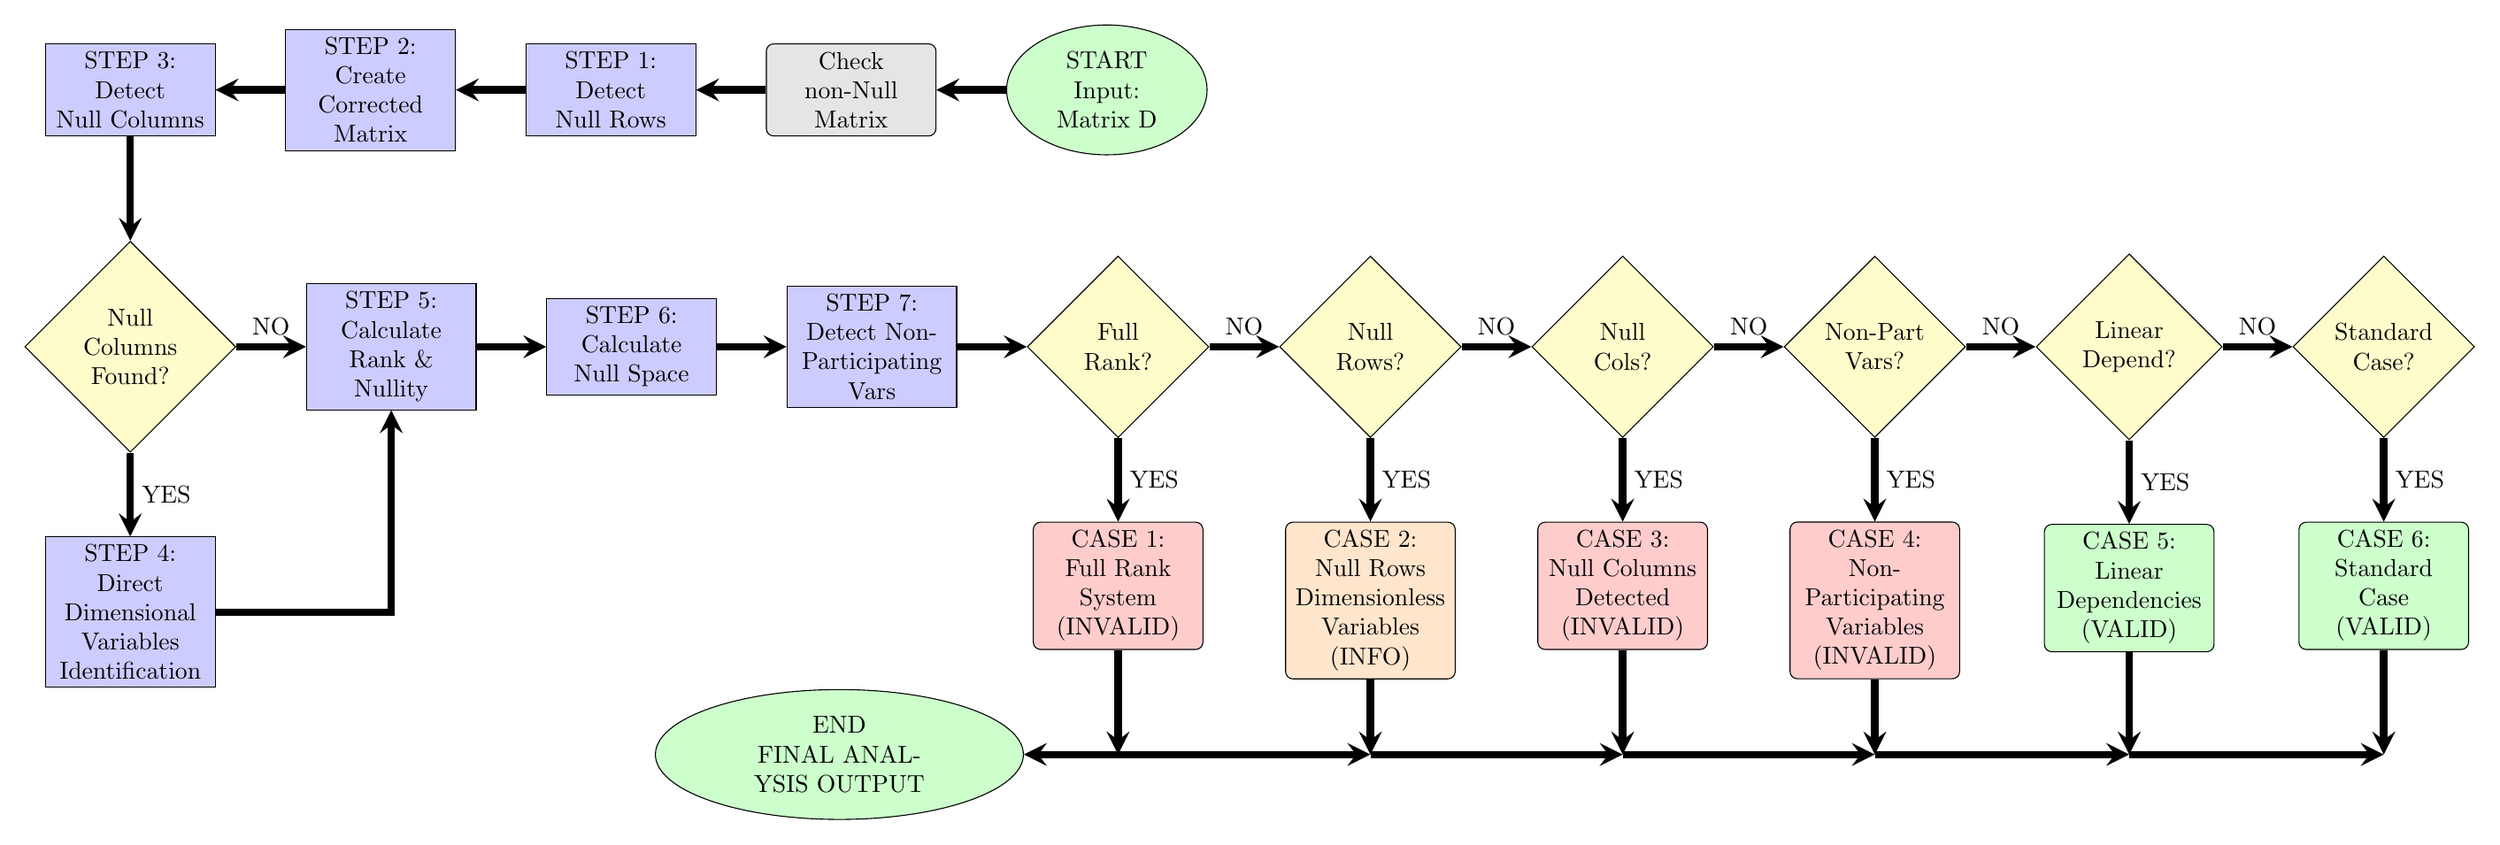
\begin{tikzpicture}[
    node distance=0.6cm and 1cm,
    auto,
    decision/.style={diamond, draw, fill=yellow!20, text width=1.8cm, text badly centered, inner sep=1pt},
    process/.style={rectangle, draw, fill=blue!20, text width=2.2cm, text centered, minimum height=0.9cm},
    terminator/.style={ellipse, draw, fill=green!20, text width=1.8cm, text centered, minimum height=0.7cm},
    finalnode/.style={ellipse, draw, fill=green!20, text width=3.5cm, text centered, minimum height=0.8cm},
    casevalid/.style={rectangle, draw, fill=green!20, text width=2.2cm, text centered, minimum height=0.9cm, rounded corners=3pt},
    caseinvalid/.style={rectangle, draw, fill=red!20, text width=2.2cm, text centered, minimum height=0.9cm, rounded corners=3pt},
    caseinfo/.style={rectangle, draw, fill=orange!20, text width=2.2cm, text centered, minimum height=0.9cm, rounded corners=3pt},
    check/.style={rectangle, draw, fill=gray!20, text width=2.2cm, text centered, minimum height=0.9cm, rounded corners=3pt},
    arrow/.style={->, >=stealth, line width=3pt}
]

% REORGANIZED CASES from left to right: 1, 2, 3, 4, 5, 6

% FIRST LEVEL (topmost): STEP 3, then STEP 2-STEP 1-CHECK-START to the right
\node [process] (step3) {STEP 3:\\Detect\\Null Columns};
\node [process, right=of step3] (step2) {STEP 2:\\Create\\Corrected Matrix};
\node [process, right=of step2] (step1) {STEP 1:\\Detect\\Null Rows};
\node [check, right=of step1] (check) {Check\\non-Null Matrix};
\node [terminator, right=of check] (start) {START\\Input: Matrix D};

% SECOND LEVEL: Decision 1 below STEP 3
\node [decision, below=1.5cm of step3] (dec1) {Null\\Columns\\Found?};

% STEP 4 below the diamond
\node [process, below=1.2cm of dec1] (step4) {STEP 4:\\Direct Dimensional\\Variables Identification};

% SECOND LEVEL continuation: Rest of the flow to the right of the diamond - REORGANIZED
\node [process, right=of dec1] (step5) {STEP 5:\\Calculate\\Rank \& Nullity};
\node [process, right=of step5] (step6) {STEP 6:\\Calculate\\Null Space};
\node [process, right=of step6] (step7) {STEP 7:\\Detect Non-\\Participating Vars};

% Decision Tree for Cases - REORGANIZED in order 1-6
\node [decision, right=of step7] (dec1case) {Full\\Rank?}; % For Case 1

% Case 1 (BELOW the diamond) - LEFT MOST
\node [caseinvalid, below=1.2cm of dec1case] (case1) {CASE 1:\\Full Rank System\\(INVALID)};

% Decision for Case 2
\node [decision, right=of dec1case] (dec2case) {Null\\Rows?}; % For Case 2

% Case 2 (BELOW the diamond)
\node [caseinfo, below=1.2cm of dec2case] (case2) {CASE 2:\\Null Rows\\Dimensionless\\Variables\\(INFO)};

% Decision for Case 3
\node [decision, right=of dec2case] (dec3case) {Null\\Cols?}; % For Case 3

% Case 3 (BELOW the diamond)
\node [caseinvalid, below=1.2cm of dec3case] (case3) {CASE 3:\\Null Columns\\Detected\\(INVALID)};

% Decision for Case 4
\node [decision, right=of dec3case] (dec4case) {Non-Part\\Vars?}; % For Case 4

% Case 4 (BELOW the diamond)
\node [caseinvalid, below=1.2cm of dec4case] (case4) {CASE 4:\\Non-Participating\\Variables\\(INVALID)};

% Decision for Case 5
\node [decision, right=of dec4case] (dec5case) {Linear\\Depend?}; % For Case 5

% Case 5 (BELOW the diamond)
\node [casevalid, below=1.2cm of dec5case] (case5) {CASE 5:\\Linear\\Dependencies\\(VALID)};

% Decision for Case 6
\node [decision, right=of dec5case] (dec6case) {Standard\\Case?}; % For Case 6

% Case 6 (BELOW the diamond) - RIGHT MOST
\node [casevalid, below=1.2cm of dec6case] (case6) {CASE 6:\\Standard Case\\(VALID)};

% COMMON HORIZONTAL LEVEL COORDINATE
\coordinate (commonLevel) at ($(case6.south) + (0,-1.5cm)$);

% VERTICAL CONNECTIONS TO COMMON LEVEL - all ending at same height with arrows
\draw [arrow] (case1.south) -- (case1.south |- commonLevel) coordinate (c1bottom);
\draw [arrow] (case2.south) -- (case2.south |- commonLevel) coordinate (c2bottom);
\draw [arrow] (case3.south) -- (case3.south |- commonLevel) coordinate (c3bottom);
\draw [arrow] (case4.south) -- (case4.south |- commonLevel) coordinate (c4bottom);
\draw [arrow] (case5.south) -- (case5.south |- commonLevel) coordinate (c5bottom);
\draw [arrow] (case6.south) -- (case6.south |- commonLevel) coordinate (c6bottom);

% Final Analysis - positioned at the SAME HEIGHT as c1bottom but to the left
\node [finalnode] at ($(c1bottom) - (4cm,0)$) (end) {END\\FINAL ANALYSIS OUTPUT};

% Main flow arrows FIRST LEVEL
\draw [arrow] (start) -- (check);
\draw [arrow] (check) -- (step1);
\draw [arrow] (step1) -- (step2);
\draw [arrow] (step2) -- (step3);

% Arrow from STEP 3 downward to the diamond
\draw [arrow] (step3) -- (dec1);

% Arrows from the diamond to STEP 4 and STEP 5
\draw [arrow] (dec1.south) -- node[right] {YES} (step4.north);
\draw [arrow] (dec1.east) -- node[above] {NO} (step5.west);

% Connection from STEP 4 to STEP 5
\draw [arrow] (step4.east) -| (step5.south);

% Main horizontal flow SECOND LEVEL - REORGANIZED
\draw [arrow] (step5) -- (step6);
\draw [arrow] (step6) -- (step7);
\draw [arrow] (step7) -- (dec1case);
\draw [arrow] (dec1case) -- node[above] {NO} (dec2case);
\draw [arrow] (dec2case) -- node[above] {NO} (dec3case);
\draw [arrow] (dec3case) -- node[above] {NO} (dec4case);
\draw [arrow] (dec4case) -- node[above] {NO} (dec5case);
\draw [arrow] (dec5case) -- node[above] {NO} (dec6case);

% Case decision arrows (DOWNWARD as requested) - REORGANIZED
\draw [arrow] (dec1case.south) -- node[right] {YES} (case1.north);
\draw [arrow] (dec2case.south) -- node[right] {YES} (case2.north);
\draw [arrow] (dec3case.south) -- node[right] {YES} (case3.north);
\draw [arrow] (dec4case.south) -- node[right] {YES} (case4.north);
\draw [arrow] (dec5case.south) -- node[right] {YES} (case5.north);
\draw [arrow] (dec6case.south) -- node[right] {YES} (case6.north);

% HORIZONTAL CONNECTIONS at common level - from left to right: 1→2→3→4→5→6
\draw [arrow] (c1bottom) -- (c2bottom);
\draw [arrow] (c2bottom) -- (c3bottom);
\draw [arrow] (c3bottom) -- (c4bottom);
\draw [arrow] (c4bottom) -- (c5bottom);
\draw [arrow] (c5bottom) -- (c6bottom);

% Final HORIZONTAL arrow from Case 1 connection point to RIGHT side of END ellipse
\draw [arrow] (c1bottom) -- (end.east);

\end{tikzpicture}
}
%\includegraphics[width=0.8\textwidth]{BuckinghamThOrganigram.pdf}
\caption{\label{fig:buckinghamflowchart} Decision flowchart for analyzing dimensional matrices in Buckingham $\pi$ theorem applications. The algorithm systematically checks for special cases and determines whether the analysis will yield valid or problematic results.}
\centering
\href{http://enriquecastilloron.github.io/PRUEBA/ObtainPiTerms_Flexible_LinearBUENO8u.html}{\underline{Click to open application}}.
\end{figure}

\subsection{Educational Implications}\index{Sectioning!Subsections}

Understanding these cases is crucial for engineering students learning dimensional analysis because:

\begin{enumerate}
    \item \textbf{Problem Formulation Skills:} Students learn to identify when their problem setup is incomplete or incorrect.
    \item \textbf{Physical Insight:} Each case type provides insight into the underlying physical relationships.
    \item \textbf{Mathematical Rigor:} Students understand the mathematical foundations behind the Buckingham $\pi$ theorem.
    \item \textbf{Practical Application:} Real engineering problems often exhibit these special cases, making this knowledge directly applicable.
\end{enumerate}

\subsection{Summary}\index{Sectioning!Subsections}

The systematic classification of cases in Buckingham $\pi$ theorem analysis provides a robust framework for handling all scenarios that arise in engineering dimensional analysis. By understanding the mathematical characteristics and physical implications of each case, engineers can:

\begin{itemize}
    \item Identify and resolve problematic problem formulations
    \item Extract maximum insight from valid analyses
    \item Apply appropriate solution strategies for each case type
    \item Develop more sophisticated understanding of dimensional relationships
\end{itemize}

This comprehensive approach ensures that dimensional analysis becomes a reliable and powerful tool in engineering design and analysis, capable of handling the complexity and variety of real-world engineering systems.


\section{\index{Sectioning!Sections}Buckingham Pi Theorem Calculator: A Comprehensive Platform}

The \textbf{Buckingham $\pi$ Theorem Calculator Enhanced} represents a paradigmatic advancement in computational dimensional analysis, integrating classical mathematical theory with modern computational methodologies to provide an unprecedented platform for systematic dimensional analysis. This sophisticated web-based application implements the fundamental principles established by Edgar Buckingham in 1914, transforming complex multi-variable physical systems into their essential dimensionless parameter sets through rigorous linear algebraic operations.

\section{Mathematical and Theoretical Framework}
\subsection{Fundamental Theorem Implementation}

The Buckingham $\pi$ theorem constitutes a cornerstone of dimensional analysis, asserting that any physically meaningful relationship among $n$ dimensional variables can be equivalently expressed as a relationship among $p = n - k$ dimensionless variables, where $k$ represents the number of fundamental physical dimensions in the system. Mathematically, this is expressed as:
\begin{equation}
f(x_1, x_2, \ldots, x_n) = 0 \quad \Rightarrow \quad F(\pi_1, \pi_2, \ldots, \pi_p) = 0
\end{equation}
where $\pi_i$ represent dimensionless groups and $p = n - \text{rank}(\mathbf{D})$, with $\mathbf{D}$ being the dimensional matrix.

\subsection{Linear Algebraic Methodology}

The calculator constructs the dimensional matrix $\mathbf{D} \in \mathbb{R}^{k \times n}$ where each column represents the dimensional formula of a physical variable:
\begin{equation}
\mathbf{D} = \begin{bmatrix}
a_{11} & a_{12} & \cdots & a_{1n} \\
a_{21} & a_{22} & \cdots & a_{2n} \\
\vdots & \vdots & \ddots & \vdots \\
a_{k1} & a_{k2} & \cdots & a_{kn}
\end{bmatrix}
\end{equation}

where $a_{ij}$ represents the exponent of the $i$-th fundamental dimension in the $j$-th variable. The system then performs:
\begin{enumerate}
    \item \textbf{Gaussian Elimination}: Systematic row operations to achieve reduced row echelon form (RREF)
    \item \textbf{Rank Determination}: Identification of linearly independent rows
    \item \textbf{Null Space Computation}: Determination of basis vectors satisfying $\mathbf{D}\mathbf{v} = \mathbf{0}$
    \item \textbf{$\pi$ Term Construction}: Formation of dimensionless groups from null space vectors
\end{enumerate}

\subsection{\index{Sectioning!Subsections}Advanced Computational Architecture}
\subsubsection{Numerical Stability and Precision}
The implementation incorporates sophisticated numerical methods to ensure computational reliability:
\begin{itemize}
    \item \textbf{Partial Pivoting}: Selection of optimal pivot elements to minimize numerical errors in Gaussian elimination
    \item \textbf{Exact pivot condition:} $|c_{j^*}| = 1$ prevents division by small numbers
    \item \textbf{Epsilon Tolerance}: Implementation of machine precision thresholds ($\epsilon = 10^{-10}$) for zero detection
    \item \textbf{Tolerance-based Rank Determination}
    \item \textbf{Integer and Rational Arithmetic for Exact Symbolic Results}
    \item \textbf{Condition Number Monitoring}: Real-time assessment of matrix conditioning
    \item \textbf{Iterative Refinement}: Post-processing verification of dimensional consistency
\end{itemize}

\subsubsection{Multi-Dimensional Framework}
The calculator supports a four-dimensional analysis framework encompassing:
\begin{align}
\text{Mass Dimension} &\quad [M] \\
\text{Length Dimension} &\quad [L] \\
\text{Time Dimension} &\quad [T] \\
\text{Count/Cycle Dimension} &\quad [C]
\end{align}

This extended framework accommodates specialized applications in fatigue analysis, cyclic phenomena, and discrete counting processes, significantly expanding the range of analyzable physical systems.

\subsection{Professional Documentation Generation}\index{Sectioning!Subsections}
\subsubsection{Automated LaTeX Synthesis}
The platform generates comprehensive LaTeX documents incorporating:
\begin{itemize}
    \item \textbf{Problem Formulation}: Systematic presentation of variables and dimensional analysis
    \item \textbf{Mathematical Derivations}: Step-by-step matrix operations with complete transparency
    \item \textbf{Tabular Presentations}: Professional formatting of dimensional matrices and results
    \item \textbf{Equation Systems}: Proper numbering and cross-referencing of mathematical expressions
    \item \textbf{Graphical Elements}: Integration capabilities for figures and diagrams
\end{itemize}

The generated documents conform to academic publishing standards and include:
\begin{verbatim}
\documentclass{article}
\usepackage{amsmath, amssymb, array, booktabs, geometry}
\end{verbatim}
ensuring compatibility with major LaTeX distributions and journal submission requirements.

\subsection{Educational and Research Integration}
\subsubsection{Pedagogical Applications}
The calculator serves as a comprehensive educational platform providing:
\begin{itemize}
    \item \textbf{Interactive Learning}: Real-time visualization of dimensional analysis concepts
    \item \textbf{Progressive Complexity}: Examples ranging from simple pendulum to complex multi-variable systems
    \item \textbf{Error Analysis}: Guided exploration of dimensional consistency principles
    \item \textbf{Historical Context}: Integration of classical problems with modern computational methods
\end{itemize}

\subsubsection{Research and Development Applications}
Professional research applications include:
\begin{enumerate}
    \item \textbf{Model Development}: Systematic identification of governing parameters
    \item \textbf{Experimental Design}: Optimization of variable space exploration
    \item \textbf{Scale-up Procedures}: Dimensional analysis for process intensification
    \item \textbf{Correlation Development}: Foundation for empirical relationship construction
\end{enumerate}

\subsection{Technical Innovation and Implementation}\index{Sectioning!Subsections}
\subsubsection{Modern Web Technologies}
The platform leverages cutting-edge web technologies:
\begin{itemize}
    \item \textbf{JavaScript ES6+}: Modern programming paradigms with robust error handling
    \item \textbf{MathJax Integration}: Real-time mathematical rendering with LaTeX compatibility
    \item \textbf{Responsive Design}: Cross-platform compatibility with adaptive user interfaces
    \item \textbf{Progressive Web App}: Offline functionality and native app-like experience
\end{itemize}

\subsubsection{Data Management and Export}
The system provides comprehensive data management capabilities:
\begin{align}
\text{JSON Export} &\quad \text{(structured data interchange)} \\
\text{LaTeX Export} &\quad \text{(publication-ready documents)} \\
\text{Session Management} &\quad \text{(historical analysis tracking)} \\
\text{Collaborative Features} &\quad \text{(sharing and distribution)}
\end{align}

\subsection{Validation and Quality Assurance}\index{Sectioning!Subsections}
The calculator incorporates extensive validation mechanisms:
\begin{itemize}
    \item \textbf{Null Space Verification}: Automatic checking of $\mathbf{D}\mathbf{v} = \mathbf{0}$ for all generated vectors
    \item \textbf{Dimensional Consistency}: Real-time validation of dimensional homogeneity
    \item \textbf{Benchmark Testing}: Comparison against established dimensional analysis results
    \item \textbf{Numerical Precision}: Monitoring of computational accuracy and stability
\end{itemize}

\subsection{Future Development and Extensibility}\index{Sectioning!Subsections}
The platform architecture supports future enhancements including:
\begin{itemize}
    \item \textbf{Machine Learning Integration}: Pattern recognition in dimensional relationships
    \item \textbf{Extended Dimensional Systems}: Support for electromagnetic and thermodynamic dimensions
    \item \textbf{Cloud Computing}: Distributed processing for large-scale dimensional analysis
    \item \textbf{API Development}: Integration with external computational frameworks
\end{itemize}

\subsection{Conclusion}\index{Sectioning!Subsections}
The Buckingham $\pi$ Theorem Calculator Enhanced represents a significant advancement in computational dimensional analysis, combining rigorous mathematical foundations with modern computational methodologies. This platform democratizes access to sophisticated dimensional analysis capabilities, serving as an invaluable resource for education, research, and professional engineering applications. Through its comprehensive feature set, professional documentation capabilities, and extensible architecture, it establishes a new standard for dimensional analysis tools in the digital age.

The calculator's integration of classical dimensional analysis theory with modern computational methods exemplifies the evolution of engineering education and research tools, providing users with unprecedented capabilities for exploring the fundamental relationships that govern physical phenomena across diverse disciplines.


\section{ Real-World Engineering Applications}\index{Sectioning!Sections}
        This section presents the dimensional analysis for 8 physical systems using the Buckingham $\pi$ theorem. Each analysis includes the system variables, dimensional matrices, and resulting dimensionless groups.
        For each engineering application, we:
\begin{enumerate}
    \item Identify the typical physical variables involved.
    \item List their dimensions in the [M, L, T, $\Theta$, C, I] system.
    \item Confirm these are standard and commonly used in real-world engineering analyses.
    \item Highlight any potential discrepancies or non-standard choices.
\end{enumerate}


\subsection{Analysis 1: Drag Force on Sphere}
\label{sec:Drag_Force_on_Sphere}

\begin{problembox}
\textbf{Physical Problem:} Determine the drag force acting on a sphere moving through a viscous fluid at steady velocity.
\end{problembox}

This analysis examines how the drag force $F$ depends on fluid properties (density $\rho$ and dynamic viscosity $\mu$), sphere characteristics (diameter $D$), and flow conditions (velocity $v$). The problem is fundamental in fluid mechanics with diverse applications: aerodynamic design of vehicles and aircraft, particle settling in industrial separations, sediment transport in environmental systems, and drug delivery through biological fluids.



Understanding the drag force relationship enables engineers to optimize shapes for minimal resistance, predict terminal velocities of falling objects, design efficient filtration systems, and model pollutant dispersion in natural waters. The analysis also reveals the transition between viscous-dominated (Stokes) and inertia-dominated flow regimes, providing insight into when different physical mechanisms control the drag behavior. This is used in aerospace (aircraft drag), automotive (vehicle aerodynamics), and marine engineering (ship resistance). These variables are consistent across textbooks and experimental studies.

\paragraph{System Variables: } The system variables are given in this table.

\begin{table}[H]
\centering
\begin{tabular}{|c|l|r|r|r|}
\hline
\textbf{Variable} & \textbf{Description} & \textbf{[M]} & \textbf{[L]} & \textbf{[T]} \\
\hline
$F$ & Drag force & 1 & 1 & -2 \\
$\rho$ & Fluid density & 1 & -3 & 0 \\
$v$ & Velocity & 0 & 1 & -1 \\
$D$ & Sphere diameter & 0 & 1 & 0 \\
$\mu$ & Dynamic viscosity & 1 & -1 & -1 \\

\hline
\end{tabular}
\caption{Variables and dimensions for Drag Force on Sphere}
\end{table}

The dimensional analysis has been performed using the methods described previously to identify the dimensionless $\pi$ parameters that govern this problem. The key parameters of the analysis are summarized below.

\paragraph{Analysis Summary}
\begin{itemize}
\item Number of variables: $n = 5$
\item Number of dimensions: $m = 3$
\item Matrix rank: $k = 3$
\item Number of $\pi$ terms: $n - k = 2$
\end{itemize}

\paragraph{Analysis Status}
System status: \textcolor{orange}{\textbf{VALID}} - Case 6: Standard Case: The system is valid and produces meaningful dimensionless $\pi$ terms.


\paragraph{Variable Classification}
\begin{itemize}
\item \textbf{Pivot columns:} 1, 2, 3
\item \textbf{Basic variables:} $F$, $\rho$, $v$
\item \textbf{Free variables:} $D$, $\mu$
\end{itemize}

                \paragraph{Dimensional Matrices}
                The homogeneous linear system generated from the original dimensional matrix $\mathbf{D}$ has been solved to obtain the basis vectors for the solution null space.

                \textbf{Original Dimensional Matrix $\mathbf{D}$:}
                \[\mathbf{D} = \begin{array}{r|rrr}
                & \text{[}M\text{]} & \text{[}L\text{]} & \text{[}T\text{]} \\
                \hline
                F & 1 & 1 & -2 \\
\rho & 1 & -3 & 0 \\
v & 0 & 1 & -1 \\
D & 0 & 1 & 0 \\
\mu & 1 & -1 & -1 \\

                \end{array}\]


        \textbf{Final Matrix $\mathbf{B}$:}
        \[\mathbf{B} = \begin{array}{r|rrrrr}
        & Pivot & Pivot & Pivot & \pi_{1} & \pi_{2} \\
        \hline
        F & 1.50 & 0.50 & 0.50 & -0.50 & -0.50 \\
\rho & -0.50 & -0.50 & -0.50 & 0.50 & -0.50 \\
v & -3 & -1 & -2 & 1 & 0 \\
D & 0 & 0 & 0 & 1 & 0 \\
\mu & 0 & 0 & 0 & 0 & 1 \\

        \end{array}\]

        \paragraph{Dimensionless $\pi$ Terms: }
        The resulting dimensionless groups that characterize this example are:
\begin{equation}
\pi_{1} = \frac{\rho \, v^{2} \, D^{2}}{F}
\end{equation}
\begin{equation}
\pi_{2} = \frac{\mu^{2}}{F \, \rho}
\end{equation}

                    \paragraph{Functional Relationship}
                    The general relationship governing this problem is:
                    \begin{equation}
                    \pi_1 = f(\pi_2)
                    \end{equation}

                    This relationship must be determined through experimental data or additional theoretical analysis to establish the associated model.


\subsection{Analysis 2: Simple Pendulum Period}
\label{sec:Simple_Pendulum_Period}

\begin{problembox}
\textbf{Physical Problem:} Determine the oscillation period of a simple pendulum under small angle approximations.
\end{problembox}

This system examines how the period $T$ depends on pendulum length $L$, gravitational acceleration $g$, and mass $m$. The dimensional analysis reveals a fundamental insight: the period is independent of mass, demonstrating the universality of gravitational motion. This result connects to Galileo's principle of equivalence and forms the basis for precision timekeeping devices.



The analysis extends beyond simple pendulums to compound pendulums, torsional oscillators, and seismic detection systems. Understanding the $T \propto \sqrt{L/g}$ scaling law enables the design of pendulum clocks, earthquake monitoring instruments, and gravitational measurement devices. The mass independence also explains why pendulum-based gravimeters can measure local gravitational variations without calibration for different test masses, making them valuable tools in geophysics and resource exploration.  This is standard in physics and mechanical engineering for pendulum dynamics. The small-angle approximation simplifies the analysis, and $Theta$ is included only for large oscillations.

\paragraph{System Variables: } The system variables are given in this table.

\begin{table}[H]
\centering
\begin{tabular}{|c|l|r|r|r|}
\hline
\textbf{Variable} & \textbf{Description} & \textbf{[M]} & \textbf{[L]} & \textbf{[T]} \\
\hline
$T$ & Oscillation period & 0 & 0 & 1 \\
$L$ & Pendulum length & 0 & 1 & 0 \\
$g$ & Gravitational acceleration & 0 & 1 & -2 \\
$m$ & Pendulum mass & 1 & 0 & 0 \\

\hline
\end{tabular}
\caption{Variables and dimensions for Simple Pendulum Period}
\end{table}

The dimensional analysis has been performed using the methods described previously to identify the dimensionless $\pi$ parameters that govern this problem. The key parameters of the analysis are summarized below.

\paragraph{Analysis Summary}
\begin{itemize}
\item Number of variables: $n = 4$
\item Number of dimensions: $m = 3$
\item Matrix rank: $k = 3$
\item Number of $\pi$ terms: $n - k = 1$
\end{itemize}

\paragraph{Analysis Status}
System status: \textcolor{red}{\textbf{ERROR}} - Case 4: Non-Participating Variables: Some variables do not participate in any $\pi$ term. This is an error - all dimensional variables must participate.

\textbf{Note:} This analysis contains configuration errors and cannot produce valid $\pi$ terms.


\paragraph{Variable Classification}
\begin{itemize}
\item \textbf{Pivot columns:} 4, 2, 1
\item \textbf{Basic variables:} $m$, $L$, $T$
\item \textbf{Free variables:} $g$
\end{itemize}

                \paragraph{Dimensional Matrices}
                The homogeneous linear system generated from the original dimensional matrix $\mathbf{D}$ has been solved to obtain the basis vectors for the solution null space.

                \textbf{Original Dimensional Matrix $\mathbf{D}$:}
                \[\mathbf{D} = \begin{array}{r|rrr}
                & \text{[}M\text{]} & \text{[}L\text{]} & \text{[}T\text{]} \\
                \hline
                T & 0 & 0 & 1 \\
L & 0 & 1 & 0 \\
g & 0 & 1 & -2 \\
m & 1 & 0 & 0 \\

                \end{array}\]


        \textbf{Final Matrix $\mathbf{B}$:}
        \[\mathbf{B} = \begin{array}{r|rrrr}
        & Pivot & Pivot & \pi_{1} & Pivot \\
        \hline
        T & 1 & 0 & 2 & 0 \\
L & 0 & 1 & -1 & 0 \\
g & 0 & 0 & 1 & 0 \\
m & 0 & 0 & 0 & 1 \\

        \end{array}\]

        \paragraph{Dimensionless $\pi$ Terms: }
        \textit{No dimensionless $\pi$ terms were generated due to configuration errors identified above.}


\subsection{Analysis 3: Basic Fatigue Analysis}
\label{sec:Basic_Fatigue_Analysis}

\begin{problembox}
\textbf{Physical Problem:} Analyze the relationship between stress levels and fatigue life in materials under cyclic loading.
\end{problembox}

This system examines how the number of cycles to failure $N$ depends on minimum stress $\sigma_{min}$ and maximum stress $\sigma_{max}$. The dimensional analysis reveals the fundamental scaling relationships underlying S-N curves (Wohler curves) and connects to Paris' law for crack propagation. Understanding these relationships enables prediction of component lifetime and optimization of stress ratios for enhanced durability.



The analysis extends to mean stress effects, stress concentration factors, and variable amplitude loading encountered in real applications. Critical insights include the roles of stress range $(\sigma_{max} - \sigma_{min})$ and stress ratio $R = \sigma_{min}/\sigma_{max}$ in determining fatigue behavior. This framework supports design methodologies for offshore structures, wind turbines, bridges, and biomedical implants, where accurate fatigue life prediction prevents catastrophic failures and enables condition-based maintenance strategies.  This is common in aerospace (aircraft components), civil engineering (bridges), and mechanical engineering (machine parts). The variables are standard but context-dependent.

\paragraph{System Variables: } The system variables are given in this table.

\begin{table}[H]
\centering
\begin{tabular}{|c|l|r|r|r|r|}
\hline
\textbf{Variable} & \textbf{Description} & \textbf{[M]} & \textbf{[L]} & \textbf{[T]} & \textbf{[C]} \\
\hline
$\sigma_{min}$ & Minimum stress & 1 & -1 & -2 & 0 \\
$\sigma_{max}$ & Maximum stress & 1 & -1 & -2 & 0 \\
$N$ & Number of cycles & 0 & 0 & 0 & 1 \\

\hline
\end{tabular}
\caption{Variables and dimensions for Basic Fatigue Analysis}
\end{table}

The dimensional analysis has been performed using the methods described previously to identify the dimensionless $\pi$ parameters that govern this problem. The key parameters of the analysis are summarized below.

\paragraph{Analysis Summary}
\begin{itemize}
\item Number of variables: $n = 3$
\item Number of dimensions: $m = 4$
\item Matrix rank: $k = 2$
\item Number of $\pi$ terms: $n - k = 1$
\end{itemize}

\paragraph{Analysis Status}
System status: \textcolor{red}{\textbf{ERROR}} - Case 4: Non-Participating Variables: Some variables do not participate in any $\pi$ term. This is an error - all dimensional variables must participate.

\textbf{Note:} This analysis contains configuration errors and cannot produce valid $\pi$ terms.


\paragraph{Variable Classification}
\begin{itemize}
\item \textbf{Pivot columns:} 1, 3
\item \textbf{Basic variables:} $\sigma_{min}$, $N$
\item \textbf{Free variables:} $\sigma_{max}$
\end{itemize}

                \paragraph{Dimensional Matrices}
                The homogeneous linear system generated from the original dimensional matrix $\mathbf{D}$ has been solved to obtain the basis vectors for the solution null space.

                \textbf{Original Dimensional Matrix $\mathbf{D}$:}
                \[\mathbf{D} = \begin{array}{r|rrrr}
                & \text{[}M\text{]} & \text{[}L\text{]} & \text{[}T\text{]} & \text{[}C\text{]} \\
                \hline
                \sigma_{min} & 1 & -1 & -2 & 0 \\
\sigma_{max} & 1 & -1 & -2 & 0 \\
N & 0 & 0 & 0 & 1 \\

                \end{array}\]


        \textbf{Final Matrix $\mathbf{B}$:}
        \[\mathbf{B} = \begin{array}{r|rrr}
        & Pivot & \pi_{1} & Pivot \\
        \hline
        \sigma_{min} & 1 & -1 & 0 \\
\sigma_{max} & 0 & 1 & 0 \\
N & 0 & 0 & 1 \\

        \end{array}\]

        \paragraph{Dimensionless $\pi$ Terms: }
        \textit{No dimensionless $\pi$ terms were generated due to configuration errors identified above.}


\subsection{Analysis 4: Endurance Fatigue Analysis}
\label{sec:Endurance_Fatigue_Analysis}

\begin{problembox}
\textbf{Physical Problem:} Analyze fatigue life incorporating material endurance limits and reference cycle counts for comprehensive life prediction.
\end{problembox}

This system examines how fatigue life $N$ depends on stress levels ($\sigma_{min}$, $\sigma_{max}$) relative to the endurance limit $\sigma_e$ and reference cycle count $N_0$. The dimensional analysis reveals the scaling relationships that govern the transition from finite-life to infinite-life regimes, enabling design strategies for both high-cycle fatigue (HCF) and very high-cycle fatigue (VHCF) applications.



The endurance limit concept, while idealized for steels, provides crucial design benchmarks and connects to probabilistic fatigue models where scatter factors and reliability requirements determine safe operating stresses. This framework supports fatigue-tolerant design in power generation equipment, railway infrastructure, and marine structures operating under millions of load cycles. Advanced applications include fretting fatigue analysis, multiaxial loading conditions, and environmental effects where the apparent endurance limit shifts due to corrosion, temperature, or frequency-dependent mechanisms.  These models are used in design of rotating machinery, turbines, and structural components.

\paragraph{System Variables: } The system variables are given in this table.

\begin{table}[H]
\centering
\begin{tabular}{|c|l|r|r|r|r|}
\hline
\textbf{Variable} & \textbf{Description} & \textbf{[M]} & \textbf{[L]} & \textbf{[T]} & \textbf{[C]} \\
\hline
$\sigma_e$ & Reference stress & 1 & -1 & -2 & 0 \\
$\sigma_{min}$ & Minimum stress & 1 & -1 & -2 & 0 \\
$\sigma_{max}$ & Maximum stress & 1 & -1 & -2 & 0 \\
$N_0$ & Limit number of cycles & 0 & 0 & 0 & 1 \\
$N$ & Number of cycles & 0 & 0 & 0 & 1 \\

\hline
\end{tabular}
\caption{Variables and dimensions for Endurance Fatigue Analysis}
\end{table}

The dimensional analysis has been performed using the methods described previously to identify the dimensionless $\pi$ parameters that govern this problem. The key parameters of the analysis are summarized below.

\paragraph{Analysis Summary}
\begin{itemize}
\item Number of variables: $n = 5$
\item Number of dimensions: $m = 4$
\item Matrix rank: $k = 2$
\item Number of $\pi$ terms: $n - k = 3$
\end{itemize}

\paragraph{Analysis Status}
System status: \textcolor{orange}{\textbf{VALID}} - Case 5: Linear Dependencies: Linear dependencies reduce the matrix rank, increasing the number of $\pi$ terms.


\paragraph{Variable Classification}
\begin{itemize}
\item \textbf{Pivot columns:} 1, 4
\item \textbf{Basic variables:} $\sigma_e$, $N_0$
\item \textbf{Free variables:} $\sigma_{min}$, $\sigma_{max}$, $N$
\end{itemize}

                \paragraph{Dimensional Matrices}
                The homogeneous linear system generated from the original dimensional matrix $\mathbf{D}$ has been solved to obtain the basis vectors for the solution null space.

                \textbf{Original Dimensional Matrix $\mathbf{D}$:}
                \[\mathbf{D} = \begin{array}{r|rrrr}
                & \text{[}M\text{]} & \text{[}L\text{]} & \text{[}T\text{]} & \text{[}C\text{]} \\
                \hline
                \sigma_e & 1 & -1 & -2 & 0 \\
\sigma_{min} & 1 & -1 & -2 & 0 \\
\sigma_{max} & 1 & -1 & -2 & 0 \\
N_0 & 0 & 0 & 0 & 1 \\
N & 0 & 0 & 0 & 1 \\

                \end{array}\]


        \textbf{Final Matrix $\mathbf{B}$:}
        \[\mathbf{B} = \begin{array}{r|rrrrr}
        & Pivot & \pi_{1} & \pi_{2} & Pivot & \pi_{3} \\
        \hline
        \sigma_e & 1 & -1 & -1 & 0 & 0 \\
\sigma_{min} & 0 & 1 & 0 & 0 & 0 \\
\sigma_{max} & 0 & 0 & 1 & 0 & 0 \\
N_0 & 0 & 0 & 0 & 1 & -1 \\
N & 0 & 0 & 0 & 0 & 1 \\

        \end{array}\]

        \paragraph{Dimensionless $\pi$ Terms: }
        The resulting dimensionless groups that characterize this example are:
\begin{equation}
\pi_{1} = \frac{\sigma_{min}}{\sigma_e}
\end{equation}
\begin{equation}
\pi_{2} = \frac{\sigma_{max}}{\sigma_e}
\end{equation}
\begin{equation}
\pi_{3} = \frac{N}{N_0}
\end{equation}

                    \paragraph{Functional Relationship}
                    The general relationship governing this problem is:
                    \begin{equation}
                    \pi_1 = f(\pi_2,\pi_3)
                    \end{equation}

                    This relationship must be determined through experimental data or additional theoretical analysis to establish the associated model.


\subsection{Analysis 5: Convective Heat Transfer}
\label{sec:Convective_Heat_Transfer}

\begin{problembox}
\textbf{Physical Problem:} Determine the heat transfer coefficient for forced convection over a surface in fluid flow.
\end{problembox}

This system examines how the heat transfer coefficient $h$ depends on thermal conductivity $k$, characteristic length $L$, fluid density $\rho$, velocity $v$, and specific heat $c_p$. The dimensional analysis reveals the fundamental scaling relationships underlying the Nusselt, Reynolds, and Prandtl numbers, which form the cornerstone of convective heat transfer correlations used in engineering design.



Understanding these dimensionless groups enables prediction of heat transfer rates across vastly different scales and applications: from microprocessor cooling with characteristic lengths in micrometers to industrial heat exchangers with meter-scale dimensions. The analysis connects momentum and thermal boundary layer development, explaining why high-velocity flows and high-conductivity fluids enhance heat transfer. This framework extends to natural convection (incorporating buoyancy effects), mixed convection regimes, and phase-change heat transfer, supporting the design of electronics cooling systems, power plant condensers, and renewable energy systems.

\paragraph{System Variables: } The system variables are given in this table.

\begin{table}[H]
\centering
\begin{tabular}{|c|l|r|r|r|r|}
\hline
\textbf{Variable} & \textbf{Description} & \textbf{[M]} & \textbf{[L]} & \textbf{[T]} & \textbf{[H]} \\
\hline
$h$ & Transfer coefficient & 1 & 0 & -3 & -1 \\
$k$ & Thermal conductivity & 1 & 1 & -3 & -1 \\
$L$ & Characteristic length & 0 & 1 & 0 & 0 \\
$\rho$ & Density & 1 & -3 & 0 & 0 \\
$v$ & Velocity & 0 & 1 & -1 & 0 \\
$cp$ & Specific heat & 0 & 2 & -2 & -1 \\

\hline
\end{tabular}
\caption{Variables and dimensions for Convective Heat Transfer}
\end{table}

The dimensional analysis has been performed using the methods described previously to identify the dimensionless $\pi$ parameters that govern this problem. The key parameters of the analysis are summarized below.

\paragraph{Analysis Summary}
\begin{itemize}
\item Number of variables: $n = 6$
\item Number of dimensions: $m = 4$
\item Matrix rank: $k = 4$
\item Number of $\pi$ terms: $n - k = 2$
\end{itemize}

\paragraph{Analysis Status}
System status: \textcolor{orange}{\textbf{VALID}} - Case 6: Standard Case: The system is valid and produces meaningful dimensionless $\pi$ terms.


\paragraph{Variable Classification}
\begin{itemize}
\item \textbf{Pivot columns:} 1, 2, 4, 5
\item \textbf{Basic variables:} $h$, $k$, $\rho$, $v$
\item \textbf{Free variables:} $L$, $cp$
\end{itemize}

                \paragraph{Dimensional Matrices}
                The homogeneous linear system generated from the original dimensional matrix $\mathbf{D}$ has been solved to obtain the basis vectors for the solution null space.

                \textbf{Original Dimensional Matrix $\mathbf{D}$:}
                \[\mathbf{D} = \begin{array}{r|rrrr}
                & \text{[}M\text{]} & \text{[}L\text{]} & \text{[}T\text{]} & \text{[}H\text{]} \\
                \hline
                h & 1 & 0 & -3 & -1 \\
k & 1 & 1 & -3 & -1 \\
L & 0 & 1 & 0 & 0 \\
\rho & 1 & -3 & 0 & 0 \\
v & 0 & 1 & -1 & 0 \\
cp & 0 & 2 & -2 & -1 \\

                \end{array}\]


        \textbf{Final Matrix $\mathbf{B}$:}
        \[\mathbf{B} = \begin{array}{r|rrrrrr}
        & Pivot & Pivot & \pi_{1} & Pivot & Pivot & \pi_{2} \\
        \hline
        h & -3 & -1 & 1 & -1 & -1 & -1 \\
k & 3 & 1 & -1 & 1 & 0 & 0 \\
L & 0 & 0 & 1 & 0 & 0 & 0 \\
\rho & 1 & 0 & 0 & 0 & 1 & 1 \\
v & 0 & 0 & 0 & -1 & 3 & 1 \\
cp & 0 & 0 & 0 & 0 & 0 & 1 \\

        \end{array}\]

        \paragraph{Dimensionless $\pi$ Terms: }
        The resulting dimensionless groups that characterize this example are:
\begin{equation}
\pi_{1} = \frac{h \, L}{k}
\end{equation}
\begin{equation}
\pi_{2} = \frac{\rho \, v \, cp}{h}
\end{equation}

                    \paragraph{Functional Relationship}
                    The general relationship governing this problem is:
                    \begin{equation}
                    \pi_1 = f(\pi_2)
                    \end{equation}

                    This relationship must be determined through experimental data or additional theoretical analysis to establish the associated model.


\subsection{Analysis 6: Pipe Flow Pressure Drop}
\label{sec:Pipe_Flow_Pressure_Drop}

\begin{problembox}
\textbf{Physical Problem:} Determine pressure drop in pipe flow systems for hydraulic design applications.
\end{problembox}

This system examines how pressure drop $D_P$ depends on fluid density $\rho$, average velocity $v$, pipe diameter $D$, length $L$, and surface roughness $\varepsilon$. The dimensional analysis yields the fundamental relationships underlying the Darcy-Weisbach equation and Moody diagram, connecting the friction factor to Reynolds number and relative roughness for both laminar and turbulent flow regimes.



Understanding these scaling laws enables prediction of pressure losses across diverse applications: from microfluidic devices with Reynolds numbers below unity to large-scale water distribution systems with highly turbulent flows. The analysis reveals why doubling pipe diameter reduces pressure drop by a factor of 32 for laminar flow, and explains the transition from smooth-pipe to rough-pipe behavior in turbulent flows. This framework extends to complex geometries including pipe networks, fittings, and valves, supporting the design of oil pipelines, chemical process equipment, and biomedical flow systems where precise pressure control is critical. This is applied in HVAC systems, heat exchangers, and aerospace (cooling systems).

\paragraph{System Variables: } The system variables are given in this table.

\begin{table}[H]
\centering
\begin{tabular}{|c|l|r|r|r|}
\hline
\textbf{Variable} & \textbf{Description} & \textbf{[M]} & \textbf{[L]} & \textbf{[T]} \\
\hline
$D_p$ & Pressure drop & 1 & -1 & -2 \\
$\rho$ & Density & 1 & -3 & 0 \\
$v$ & Velocity & 0 & 1 & -1 \\
$D$ & Pipe diameter & 0 & 1 & 0 \\
$L$ & Pipe length & 0 & 1 & 0 \\
$\epsilon$ & Roughness & 0 & 1 & 0 \\
$\mu$ & Viscosity & 1 & -1 & -1 \\

\hline
\end{tabular}
\caption{Variables and dimensions for Pipe Flow Pressure Drop}
\end{table}

The dimensional analysis has been performed using the methods described previously to identify the dimensionless $\pi$ parameters that govern this problem. The key parameters of the analysis are summarized below.

\paragraph{Analysis Summary}
\begin{itemize}
\item Number of variables: $n = 7$
\item Number of dimensions: $m = 3$
\item Matrix rank: $k = 3$
\item Number of $\pi$ terms: $n - k = 4$
\end{itemize}

\paragraph{Analysis Status}
System status: \textcolor{orange}{\textbf{VALID}} - Case 6: Standard Case: The system is valid and produces meaningful dimensionless $\pi$ terms.


\paragraph{Variable Classification}
\begin{itemize}
\item \textbf{Pivot columns:} 1, 2, 4
\item \textbf{Basic variables:} $D_p$, $\rho$, $D$
\item \textbf{Free variables:} $v$, $L$, $\epsilon$, $\mu$
\end{itemize}

                \paragraph{Dimensional Matrices}
                The homogeneous linear system generated from the original dimensional matrix $\mathbf{D}$ has been solved to obtain the basis vectors for the solution null space.

                \textbf{Original Dimensional Matrix $\mathbf{D}$:}
                \[\mathbf{D} = \begin{array}{r|rrr}
                & \text{[}M\text{]} & \text{[}L\text{]} & \text{[}T\text{]} \\
                \hline
                D_p & 1 & -1 & -2 \\
\rho & 1 & -3 & 0 \\
v & 0 & 1 & -1 \\
D & 0 & 1 & 0 \\
L & 0 & 1 & 0 \\
\epsilon & 0 & 1 & 0 \\
\mu & 1 & -1 & -1 \\

                \end{array}\]


        \textbf{Final Matrix $\mathbf{B}$:}
        \[\mathbf{B} = \begin{array}{r|rrrrrrr}
        & Pivot & Pivot & \pi_{1} & Pivot & \pi_{2} & \pi_{3} & \pi_{4} \\
        \hline
        D_p & 0 & 0 & -0.50 & -0.50 & 0 & 0 & -0.50 \\
\rho & 1 & 0 & 0.50 & 0.50 & 0 & 0 & -0.50 \\
v & 0 & 0 & 1 & 0 & 0 & 0 & 0 \\
D & 3 & 1 & 0 & 1 & -1 & -1 & -1 \\
L & 0 & 0 & 0 & 0 & 1 & 0 & 0 \\
\epsilon & 0 & 0 & 0 & 0 & 0 & 1 & 0 \\
\mu & 0 & 0 & 0 & 0 & 0 & 0 & 1 \\

        \end{array}\]

        \paragraph{Dimensionless $\pi$ Terms: }
        The resulting dimensionless groups that characterize this example are:
\begin{equation}
\pi_{1} = \frac{\rho \, v^{2}}{D_p}
\end{equation}
\begin{equation}
\pi_{2} = \frac{L}{D}
\end{equation}
\begin{equation}
\pi_{3} = \frac{\epsilon}{D}
\end{equation}
\begin{equation}
\pi_{4} = \frac{\mu^{2}}{D_p \, \rho \, D^{2}}
\end{equation}

                    \paragraph{Functional Relationship}
                    The general relationship governing this problem is:
                    \begin{equation}
                    \pi_1 = f(\pi_2, \ldots, \pi_{4})
                    \end{equation}

                    This relationship must be determined through experimental data or additional theoretical analysis to establish the associated model.


\subsection{Analysis 7: Thermal Expansion}
\label{sec:Thermal_Expansion}

\begin{problembox}
\textbf{Physical Problem:} Analyze dimensional changes in materials due to temperature variations.
\end{problembox}

This system examines how length change $D_L$ depends on initial length $L_0$, thermal expansion coefficient $\alpha$, and temperature change $D_T$. The dimensional analysis reveals the linear relationship $D_L = \alpha L_0 D_T$, demonstrating that thermal strain is independent of material size, a fundamental principle enabling predictable scaling from laboratory specimens to massive structures.



This scaling invariance is crucial for designing thermal expansion joints in bridges, pipelines, and buildings, where differential expansion between materials can generate enormous stresses. The analysis extends to bimetallic strips in thermostats, precision instrument design where thermal stability is critical, and semiconductor manufacturing where nanometer-scale thermal expansion affects device performance. Understanding thermal expansion also enables thermal stress analysis in composite materials, jet engine components operating across extreme temperature gradients, and space structures experiencing rapid thermal cycling between sunlit and shadowed conditions. It is used in civil engineering (bridges, buildings), mechanical engineering (machine parts), and material science.

\paragraph{System Variables: } The system variables are given in this table.

\begin{table}[H]
\centering
\begin{tabular}{|c|l|r|r|}
\hline
\textbf{Variable} & \textbf{Description} & \textbf{[L]} & \textbf{[H]} \\
\hline
$D_L$ & Length change & 1 & 0 \\
$L_0$ & Initial length & 1 & 0 \\
$\alpha$ & Thermal expansion coefficient & 0 & -1 \\
$D_T$ & Temperature change & 0 & 1 \\

\hline
\end{tabular}
\caption{Variables and dimensions for Thermal Expansion}
\end{table}

The dimensional analysis has been performed using the methods described previously to identify the dimensionless $\pi$ parameters that govern this problem. The key parameters of the analysis are summarized below.

\paragraph{Analysis Summary}
\begin{itemize}
\item Number of variables: $n = 4$
\item Number of dimensions: $m = 2$
\item Matrix rank: $k = 2$
\item Number of $\pi$ terms: $n - k = 2$
\end{itemize}

\paragraph{Analysis Status}
System status: \textcolor{orange}{\textbf{VALID}} - Case 6: Standard Case: The system is valid and produces meaningful dimensionless $\pi$ terms.


\paragraph{Variable Classification}
\begin{itemize}
\item \textbf{Pivot columns:} 1, 3
\item \textbf{Basic variables:} $D_L$, $\alpha$
\item \textbf{Free variables:} $L_0$, $D_T$
\end{itemize}

                \paragraph{Dimensional Matrices}
                The homogeneous linear system generated from the original dimensional matrix $\mathbf{D}$ has been solved to obtain the basis vectors for the solution null space.

                \textbf{Original Dimensional Matrix $\mathbf{D}$:}
                \[\mathbf{D} = \begin{array}{r|rr}
                & \text{[}L\text{]} & \text{[}H\text{]} \\
                \hline
                D_L & 1 & 0 \\
L_0 & 1 & 0 \\
\alpha & 0 & -1 \\
D_T & 0 & 1 \\

                \end{array}\]


        \textbf{Final Matrix $\mathbf{B}$:}
        \[\mathbf{B} = \begin{array}{r|rrrr}
        & Pivot & \pi_{1} & Pivot & \pi_{2} \\
        \hline
        D_L & 1 & -1 & 0 & 0 \\
L_0 & 0 & 1 & 0 & 0 \\
\alpha & 0 & 0 & -1 & 1 \\
D_T & 0 & 0 & 0 & 1 \\

        \end{array}\]

        \paragraph{Dimensionless $\pi$ Terms: }
        The resulting dimensionless groups that characterize this example are:
\begin{equation}
\pi_{1} = \frac{L_0}{D_L}
\end{equation}
\begin{equation}
\pi_{2} = \alpha \, D_T
\end{equation}

                    \paragraph{Functional Relationship}
                    The general relationship governing this problem is:
                    \begin{equation}
                    \pi_1 = f(\pi_2)
                    \end{equation}

                    This relationship must be determined through experimental data or additional theoretical analysis to establish the associated model.


\subsection{Analysis 8: Electrical Circuit (EC)}
\label{sec:Electrical_Circuit_EC}

\begin{problembox}
\textbf{Physical Problem:} Analyze the dimensional relationships in a DC electrical circuit containing resistive elements.
\end{problembox}

This system examines the fundamental electrical quantities: voltage $V$ (potential difference), current $I$ (electrical flow), resistance $R$ (opposition to current flow), power $P$ (energy transfer rate), time $t$, and electric charge $Q$. The dimensional analysis reveals how these variables combine to form dimensionless groups, providing insight into circuit scaling laws, energy efficiency relationships, and transient response characteristics.



Understanding these dimensionless relationships is essential for circuit optimization, thermal management (through power dissipation analysis), and designing circuits across different scales, from microelectronics to power systems. The analysis also illuminates the connection between Ohm's law, Joule heating, and charge-current relationships, forming the foundation for more complex circuit behaviors including RC time constants and energy storage mechanisms.

\paragraph{System Variables: } The system variables are given in this table.

\begin{table}[H]
\centering
\begin{tabular}{|c|l|r|r|r|r|}
\hline
\textbf{Variable} & \textbf{Description} & \textbf{[M]} & \textbf{[L]} & \textbf{[T]} & \textbf{[I]} \\
\hline
$V$ & Voltage & 1 & 2 & -3 & -1 \\
$I$ & Intensity & 0 & 0 & 0 & 1 \\
$R$ & Resistence & 1 & 2 & -3 & -2 \\
$P$ & Power & 1 & 2 & -3 & 0 \\
$T$ & Time & 0 & 0 & 1 & 0 \\
$Q$ & Electric charge & 0 & 0 & 1 & 1 \\

\hline
\end{tabular}
\caption{Variables and dimensions for Electrical Circuit (EC)}
\end{table}

The dimensional analysis has been performed using the methods described previously to identify the dimensionless $\pi$ parameters that govern this problem. The key parameters of the analysis are summarized below.

\paragraph{Analysis Summary}
\begin{itemize}
\item Number of variables: $n = 6$
\item Number of dimensions: $m = 4$
\item Matrix rank: $k = 3$
\item Number of $\pi$ terms: $n - k = 3$
\end{itemize}

\paragraph{Analysis Status}
System status: \textcolor{orange}{\textbf{VALID}} - Case 5: Linear Dependencies: Linear dependencies reduce the matrix rank, increasing the number of $\pi$ terms.


\paragraph{Variable Classification}
\begin{itemize}
\item \textbf{Pivot columns:} 1, 5, 2
\item \textbf{Basic variables:} $V$, $T$, $I$
\item \textbf{Free variables:} $R$, $P$, $Q$
\end{itemize}

                \paragraph{Dimensional Matrices}
                The homogeneous linear system generated from the original dimensional matrix $\mathbf{D}$ has been solved to obtain the basis vectors for the solution null space.

                \textbf{Original Dimensional Matrix $\mathbf{D}$:}
                \[\mathbf{D} = \begin{array}{r|rrrr}
                & \text{[}M\text{]} & \text{[}L\text{]} & \text{[}T\text{]} & \text{[}I\text{]} \\
                \hline
                V & 1 & 2 & -3 & -1 \\
I & 0 & 0 & 0 & 1 \\
R & 1 & 2 & -3 & -2 \\
P & 1 & 2 & -3 & 0 \\
T & 0 & 0 & 1 & 0 \\
Q & 0 & 0 & 1 & 1 \\

                \end{array}\]


        \textbf{Final Matrix $\mathbf{B}$:}
        \[\mathbf{B} = \begin{array}{r|rrrrrr}
        & Pivot & Pivot & \pi_{1} & \pi_{2} & Pivot & \pi_{3} \\
        \hline
        V & 1 & 0 & -1 & -1 & 0 & 0 \\
I & 1 & 1 & 1 & -1 & 0 & -1 \\
R & 0 & 0 & 1 & 0 & 0 & 0 \\
P & 0 & 0 & 0 & 1 & 0 & 0 \\
T & 3 & 0 & 0 & 0 & 1 & -1 \\
Q & 0 & 0 & 0 & 0 & 0 & 1 \\

        \end{array}\]

        \paragraph{Dimensionless $\pi$ Terms: }
        The resulting dimensionless groups that characterize this example are:
\begin{equation}
\pi_{1} = \frac{I \, R}{V}
\end{equation}
\begin{equation}
\pi_{2} = \frac{P}{V \, I}
\end{equation}
\begin{equation}
\pi_{3} = \frac{Q}{I \, T}
\end{equation}

                    \paragraph{Functional Relationship}
                    The general relationship governing this problem is:
                    \begin{equation}
                    \pi_1 = f(\pi_2,\pi_3)
                    \end{equation}

                    This relationship must be determined through experimental data or additional theoretical analysis to establish the associated model.


\subsection{Analysis 9: Turbulent Evaporation}
\label{sec:Turbulent_Evaporation}

\begin{problembox}
\textbf{Physical Problem:} Turbulent evaporation from a free surface in the presence of wind.
\end{problembox}

In the problem of turbulent evaporation from a free surface in the presence of wind, the following variables are considered important. The dimensions are given in brackets and expressed in terms of length $L$ and time $T$: (a) Evaporation under turbulent conditions $V_T$ $[LT^{-1}]$,  (b) Humidity difference $q_s-q$ (saturation deficit), where $q$ is the specific humidity of air and $q_s$ is the specific saturation humidity at the water surface temperature (both dimensionless), (c) Turbulent diffusion coefficient $K$ for water vapor in air $[L^2T^{-1}]$, (d) Wetted surface area $S$ $[L^2]$, (e) Mean wind velocity $U$ $[LT^{-1}]$. The influence of the different variables are analyzed.

\paragraph{System Variables: } The system variables are given in this table.

\begin{table}[H]
\centering
\begin{tabular}{|c|l|r|r|}
\hline
\textbf{Variable} & \textbf{Description} & \textbf{[L]} & \textbf{[T]} \\
\hline
$Vt$ & Evaporation rate & 1 & -1 \\
$hdif$ & Humidity difference & 0 & 0 \\
$K$ & Turbulent diffusion coefficient & 2 & -1 \\
$S$ & Surface area & 2 & 0 \\
$U$ & Wind velocity & 1 & -1 \\

\hline
\end{tabular}
\caption{Variables and dimensions for Turbulent Evaporation}
\end{table}

The dimensional analysis has been performed using the methods described previously to identify the dimensionless $\pi$ parameters that govern this problem. The key parameters of the analysis are summarized below.

\paragraph{Analysis Summary}
\begin{itemize}
\item Number of variables: $n = 5$
\item Number of dimensions: $m = 2$
\item Matrix rank: $k = 2$
\item Number of $\pi$ terms: $n - k = 3$
\end{itemize}

\paragraph{Analysis Status}
System status: \textcolor{orange}{\textbf{VALID}} - Case 2 + 6: Multiple conditions detected simultaneously.


\paragraph{Variable Classification}
\begin{itemize}
\item \textbf{Pivot columns:} 1, 3
\item \textbf{Basic variables:} $Vt$, $K$
\item \textbf{Free variables:} $hdif$, $S$, $U$
\end{itemize}

                \paragraph{Dimensional Matrices}
                The homogeneous linear system generated from the original dimensional matrix $\mathbf{D}$ has been solved to obtain the basis vectors for the solution null space.

                \textbf{Original Dimensional Matrix $\mathbf{D}$:}
                \[\mathbf{D} = \begin{array}{r|rr}
                & \text{[}L\text{]} & \text{[}T\text{]} \\
                \hline
                Vt & 1 & -1 \\
hdif & 0 & 0 \\
K & 2 & -1 \\
S & 2 & 0 \\
U & 1 & -1 \\

                \end{array}\]


        \textbf{Final Matrix $\mathbf{B}$:}
        \[\mathbf{B} = \begin{array}{r|rrrrr}
        & Pivot & \pi_{1} & Pivot & \pi_{2} & \pi_{3} \\
        \hline
        Vt & -1 & 0 & -2 & 2 & -1 \\
hdif & 0 & 1 & 0 & 0 & 0 \\
K & 1 & 0 & 1 & -2 & 0 \\
S & 0 & 0 & 0 & 1 & 0 \\
U & 0 & 0 & 0 & 0 & 1 \\

        \end{array}\]

        \paragraph{Dimensionless $\pi$ Terms: }
        The resulting dimensionless groups that characterize this example are:
\begin{equation}
\pi_{1} = hdif
\end{equation}
\begin{equation}
\pi_{2} = \frac{Vt^{2} \, S}{K^{2}}
\end{equation}
\begin{equation}
\pi_{3} = \frac{U}{Vt}
\end{equation}

                    \paragraph{Functional Relationship}
                    The general relationship governing this problem is:
                    \begin{equation}
                    \pi_1 = f(\pi_2,\pi_3)
                    \end{equation}

                    This relationship must be determined through experimental data or additional theoretical analysis to establish the associated model.


\subsection{Analysis 10: Case 1: Full Rank}
\label{sec:Case_1_Full_Rank}

\begin{problembox}
\textbf{Physical Problem:} Case 1 refers to a dimensional matrix with full rank (rank equals the number of fundamental dimensions $k$), where all dimensions are independent, and the maximum number of $\pi$ terms ($n - r$) is produced.
\end{problembox}

This is similar to the Standard case but emphasizes a scenario where the matrix has no linear dependencies among dimensions, ensuring the zero as the unique solution. It's a robust test for both calculation methods, as the Linear System Solver should yield a clean solution, and Null Space Analysis should confirm a well-defined kernel.

\paragraph{System Variables: } The system variables are given in this table.

\begin{table}[H]
\centering
\begin{tabular}{|c|l|r|r|r|}
\hline
\textbf{Variable} & \textbf{Description} & \textbf{[M]} & \textbf{[L]} & \textbf{[T]} \\
\hline
$F$ & Force & 1 & 1 & -2 \\
$m$ & Mass & 1 & 0 & 0 \\
$T$ & Time & 0 & 0 & 1 \\

\hline
\end{tabular}
\caption{Variables and dimensions for Case 1: Full Rank}
\end{table}

The dimensional analysis has been performed using the methods described previously to identify the dimensionless $\pi$ parameters that govern this problem. The key parameters of the analysis are summarized below.

\paragraph{Analysis Summary}
\begin{itemize}
\item Number of variables: $n = 3$
\item Number of dimensions: $m = 3$
\item Matrix rank: $k = 3$
\item Number of $\pi$ terms: $n - k = 0$
\end{itemize}

\paragraph{Analysis Status}
System status: \textcolor{red}{\textbf{ERROR}} - Case 1: Full Rank: The number of variables equals the matrix rank (n = r). No dimensionless $\pi$ terms can be formed.

\textbf{Note:} This analysis contains configuration errors and cannot produce valid $\pi$ terms.


\paragraph{Variable Classification}
\begin{itemize}
\item \textbf{Pivot columns:} 1, 2, 3
\item \textbf{Basic variables:} $F$, $m$, $T$
\item \textbf{Free variables:}
\end{itemize}

                \paragraph{Dimensional Matrices}
                The homogeneous linear system generated from the original dimensional matrix $\mathbf{D}$ has been solved to obtain the basis vectors for the solution null space.

                \textbf{Original Dimensional Matrix $\mathbf{D}$:}
                \[\mathbf{D} = \begin{array}{r|rrr}
                & \text{[}M\text{]} & \text{[}L\text{]} & \text{[}T\text{]} \\
                \hline
                F & 1 & 1 & -2 \\
m & 1 & 0 & 0 \\
T & 0 & 0 & 1 \\

                \end{array}\]


        \textbf{Final Matrix $\mathbf{B}$:}
        \[\mathbf{B} = \begin{array}{r|rrr}
        & Pivot & Pivot & Pivot \\
        \hline
        F & 0 & 1 & 0 \\
m & 1 & -1 & 0 \\
T & 0 & 2 & 1 \\

        \end{array}\]

        \paragraph{Dimensionless $\pi$ Terms: }
        \textit{No dimensionless $\pi$ terms were generated due to configuration errors identified above.}


\subsection{Analysis 11: Case 2: Null Row (Dimensionless Variable)}
\label{sec:Case_2_Null_Row_Dimensionless_Variable}

\begin{problembox}
\textbf{Physical Problem:} Case 2 involves a dimensional matrix with one or more row of zeros, indicating that a variable is dimensionless or has no dimensional contribution (e.g., an angle in radians or a pure number like a proportion or percentile).
\end{problembox}

This case tests the calculator's handling of variables that are already dimensionless, which should appear directly as $\pi$ terms without further manipulation. For example, a proportiom, a percentile or the angles (all dimensionless) create null rows. The Linear System Solver should identify these trivially, while Null Space Analysis should confirm the variable's independence from the kernel.

\paragraph{System Variables: } The system variables are given in this table.

\begin{table}[H]
\centering
\begin{tabular}{|c|l|r|r|r|}
\hline
\textbf{Variable} & \textbf{Description} & \textbf{[M]} & \textbf{[L]} & \textbf{[T]} \\
\hline
$F$ & Force & 1 & 1 & -2 \\
$v$ & Velocity & 0 & 1 & -1 \\
$L$ & Length & 0 & 1 & 0 \\
$Re$ & Reynolds number & 0 & 0 & 0 \\

\hline
\end{tabular}
\caption{Variables and dimensions for Case 2: Null Row (Dimensionless Variable)}
\end{table}

The dimensional analysis has been performed using the methods described previously to identify the dimensionless $\pi$ parameters that govern this problem. The key parameters of the analysis are summarized below.

\paragraph{Analysis Summary}
\begin{itemize}
\item Number of variables: $n = 4$
\item Number of dimensions: $m = 3$
\item Matrix rank: $k = 3$
\item Number of $\pi$ terms: $n - k = 1$
\end{itemize}

\paragraph{Analysis Status}
System status: \textcolor{red}{\textbf{ERROR}} - Case 2 + 4: Multiple conditions detected simultaneously.

\textbf{Note:} This analysis contains configuration errors and cannot produce valid $\pi$ terms.


\paragraph{Variable Classification}
\begin{itemize}
\item \textbf{Pivot columns:} 1, 2, 3
\item \textbf{Basic variables:} $F$, $v$, $L$
\item \textbf{Free variables:} $Re$
\end{itemize}

                \paragraph{Dimensional Matrices}
                The homogeneous linear system generated from the original dimensional matrix $\mathbf{D}$ has been solved to obtain the basis vectors for the solution null space.

                \textbf{Original Dimensional Matrix $\mathbf{D}$:}
                \[\mathbf{D} = \begin{array}{r|rrr}
                & \text{[}M\text{]} & \text{[}L\text{]} & \text{[}T\text{]} \\
                \hline
                F & 1 & 1 & -2 \\
v & 0 & 1 & -1 \\
L & 0 & 1 & 0 \\
Re & 0 & 0 & 0 \\

                \end{array}\]


        \textbf{Final Matrix $\mathbf{B}$:}
        \[\mathbf{B} = \begin{array}{r|rrrr}
        & Pivot & Pivot & Pivot & \pi_{1} \\
        \hline
        F & 1 & 0 & 0 & 0 \\
v & -2 & 0 & -1 & 0 \\
L & 1 & 1 & 1 & 0 \\
Re & 0 & 0 & 0 & 1 \\

        \end{array}\]

        \paragraph{Dimensionless $\pi$ Terms: }
        \textit{No dimensionless $\pi$ terms were generated due to configuration errors identified above.}


\subsection{Analysis 12: Case 3: Null Column}
\label{sec:Case_3_Null_Column}

\begin{problembox}
\textbf{Physical Problem:} Case 3 represents a dimensional matrix with some column of zeros, meaning one or more dimensions (e.g., M, T, X) are not present in any variable. This could occur in problems where a fundamental dimension is irrelevant (e.g., no temperature in a mechanical system).
\end{problembox}

This tests the calculator's ability to handle reduced dimensionality. For instance, in a purely geometric problem (e.g., scaling of shapes), only length [L] might appear, creating zero columns for M, T, etc. The calculator should adjust the rank calculation and produce fewer $\pi$ terms than expected.

\paragraph{System Variables: } The system variables are given in this table.

\begin{table}[H]
\centering
\begin{tabular}{|c|l|r|r|r|r|}
\hline
\textbf{Variable} & \textbf{Description} & \textbf{[M]} & \textbf{[L]} & \textbf{[T]} & \textbf{[X]} \\
\hline
$F$ & Force & 1 & 1 & -2 & 0 \\
$v$ & Velocity & 0 & 1 & -1 & 0 \\
$L$ & Length & 0 & 1 & 0 & 0 \\
$\rho$ & Density & 1 & -3 & 0 & 0 \\

\hline
\end{tabular}
\caption{Variables and dimensions for Case 3: Null Column}
\end{table}

The dimensional analysis has been performed using the methods described previously to identify the dimensionless $\pi$ parameters that govern this problem. The key parameters of the analysis are summarized below.

\paragraph{Analysis Summary}
\begin{itemize}
\item Number of variables: $n = 4$
\item Number of dimensions: $m = 4$
\item Matrix rank: $k = 3$
\item Number of $\pi$ terms: $n - k = 1$
\end{itemize}

\paragraph{Analysis Status}
System status: \textcolor{red}{\textbf{ERROR}} - Case 3: Null Columns: The dimensional matrix contains one or more null columns. This indicates redundant or invalid dimensions.

\textbf{Note:} This analysis contains configuration errors and cannot produce valid $\pi$ terms.


\paragraph{Variable Classification}
\begin{itemize}
\item \textbf{Pivot columns:} 1, 2, 3
\item \textbf{Basic variables:} $F$, $v$, $L$
\item \textbf{Free variables:} $\rho$
\end{itemize}

                \paragraph{Dimensional Matrices}
                The homogeneous linear system generated from the original dimensional matrix $\mathbf{D}$ has been solved to obtain the basis vectors for the solution null space.

                \textbf{Original Dimensional Matrix $\mathbf{D}$:}
                \[\mathbf{D} = \begin{array}{r|rrrr}
                & \text{[}M\text{]} & \text{[}L\text{]} & \text{[}T\text{]} & \text{[}X\text{]} \\
                \hline
                F & 1 & 1 & -2 & 0 \\
v & 0 & 1 & -1 & 0 \\
L & 0 & 1 & 0 & 0 \\
\rho & 1 & -3 & 0 & 0 \\

                \end{array}\]


        \textbf{Final Matrix $\mathbf{B}$:}
        \[\mathbf{B} = \begin{array}{r|rrrr}
        & Pivot & Pivot & Pivot & \pi_{1} \\
        \hline
        F & 1 & 0 & 0 & -1 \\
v & -2 & 0 & -1 & 2 \\
L & 1 & 1 & 1 & 2 \\
\rho & 0 & 0 & 0 & 1 \\

        \end{array}\]

        \paragraph{Dimensionless $\pi$ Terms: }
        \textit{No dimensionless $\pi$ terms were generated due to configuration errors identified above.}


\subsection{Analysis 13: Case 4: Non-Participating Variable}
\label{sec:Case_4_NonParticipating_Variable}

\begin{problembox}
\textbf{Physical Problem:} Case 4 represents variables that do not contribute to the final $\pi$ terms, often because they cancel out or are irrelevant to the physical relationship (e.g., mass in a simple pendulum's period).
\end{problembox}

This tests the calculator's ability to identify variables that, while included, have no effect on the dimensionless groups. For example, in a pendulum, the mass of the bob is often included but found to be non-participating after analysis. Both methods should correctly exclude such variables from the $\pi$ terms.

\paragraph{System Variables: } The system variables are given in this table.

\begin{table}[H]
\centering
\begin{tabular}{|c|l|r|r|r|}
\hline
\textbf{Variable} & \textbf{Description} & \textbf{[M]} & \textbf{[L]} & \textbf{[T]} \\
\hline
$v$ & Velocity & 0 & 1 & -1 \\
$L$ & Length & 0 & 1 & 0 \\
$t$ & Time & 0 & 0 & 1 \\
$m$ & Mass & 1 & 0 & 0 \\

\hline
\end{tabular}
\caption{Variables and dimensions for Case 4: Non-Participating Variable}
\end{table}

The dimensional analysis has been performed using the methods described previously to identify the dimensionless $\pi$ parameters that govern this problem. The key parameters of the analysis are summarized below.

\paragraph{Analysis Summary}
\begin{itemize}
\item Number of variables: $n = 4$
\item Number of dimensions: $m = 3$
\item Matrix rank: $k = 3$
\item Number of $\pi$ terms: $n - k = 1$
\end{itemize}

\paragraph{Analysis Status}
System status: \textcolor{red}{\textbf{ERROR}} - Case 4: Non-Participating Variables: Some variables do not participate in any $\pi$ term. This is an error - all dimensional variables must participate.

\textbf{Note:} This analysis contains configuration errors and cannot produce valid $\pi$ terms.


\paragraph{Variable Classification}
\begin{itemize}
\item \textbf{Pivot columns:} 4, 1, 2
\item \textbf{Basic variables:} $m$, $v$, $L$
\item \textbf{Free variables:} $t$
\end{itemize}

                \paragraph{Dimensional Matrices}
                The homogeneous linear system generated from the original dimensional matrix $\mathbf{D}$ has been solved to obtain the basis vectors for the solution null space.

                \textbf{Original Dimensional Matrix $\mathbf{D}$:}
                \[\mathbf{D} = \begin{array}{r|rrr}
                & \text{[}M\text{]} & \text{[}L\text{]} & \text{[}T\text{]} \\
                \hline
                v & 0 & 1 & -1 \\
L & 0 & 1 & 0 \\
t & 0 & 0 & 1 \\
m & 1 & 0 & 0 \\

                \end{array}\]


        \textbf{Final Matrix $\mathbf{B}$:}
        \[\mathbf{B} = \begin{array}{r|rrrr}
        & Pivot & Pivot & \pi_{1} & Pivot \\
        \hline
        v & 0 & -1 & 1 & 0 \\
L & 1 & 1 & -1 & 0 \\
t & 0 & 0 & 1 & 0 \\
m & 0 & 0 & 0 & 1 \\

        \end{array}\]

        \paragraph{Dimensionless $\pi$ Terms: }
        \textit{No dimensionless $\pi$ terms were generated due to configuration errors identified above.}


\subsection{Analysis 14: Case 5: Linear Dependencies}
\label{sec:Case_5_Linear_Dependencies}

\begin{problembox}
\textbf{Physical Problem:} Linear Dependencies
\end{problembox}

This example corresponds to the Linear Dependencies case

\paragraph{System Variables: } The system variables are given in this table.

\begin{table}[H]
\centering
\begin{tabular}{|c|l|r|r|r|}
\hline
\textbf{Variable} & \textbf{Description} & \textbf{[M]} & \textbf{[L]} & \textbf{[T]} \\
\hline
$F$ & Force & 1 & 1 & -2 \\
$F0$ & Initial force & 1 & 1 & -2 \\
$E$ & Energy & 1 & 2 & -2 \\
$L$ & Length & 0 & 1 & 0 \\
$L_0$ & Reflength & 0 & 1 & 0 \\

\hline
\end{tabular}
\caption{Variables and dimensions for Case 5: Linear Dependencies}
\end{table}

The dimensional analysis has been performed using the methods described previously to identify the dimensionless $\pi$ parameters that govern this problem. The key parameters of the analysis are summarized below.

\paragraph{Analysis Summary}
\begin{itemize}
\item Number of variables: $n = 5$
\item Number of dimensions: $m = 3$
\item Matrix rank: $k = 2$
\item Number of $\pi$ terms: $n - k = 3$
\end{itemize}

\paragraph{Analysis Status}
System status: \textcolor{orange}{\textbf{VALID}} - Case 5: Linear Dependencies: Linear dependencies reduce the matrix rank, increasing the number of $\pi$ terms.


\paragraph{Variable Classification}
\begin{itemize}
\item \textbf{Pivot columns:} 1, 3
\item \textbf{Basic variables:} $F$, $E$
\item \textbf{Free variables:} $F0$, $L$, $L_0$
\end{itemize}

                \paragraph{Dimensional Matrices}
                The homogeneous linear system generated from the original dimensional matrix $\mathbf{D}$ has been solved to obtain the basis vectors for the solution null space.

                \textbf{Original Dimensional Matrix $\mathbf{D}$:}
                \[\mathbf{D} = \begin{array}{r|rrr}
                & \text{[}M\text{]} & \text{[}L\text{]} & \text{[}T\text{]} \\
                \hline
                F & 1 & 1 & -2 \\
F0 & 1 & 1 & -2 \\
E & 1 & 2 & -2 \\
L & 0 & 1 & 0 \\
L_0 & 0 & 1 & 0 \\

                \end{array}\]


        \textbf{Final Matrix $\mathbf{B}$:}
        \[\mathbf{B} = \begin{array}{r|rrrrr}
        & Pivot & \pi_{1} & Pivot & \pi_{2} & \pi_{3} \\
        \hline
        F & 2 & -1 & -1 & 1 & 1 \\
F0 & 0 & 1 & 0 & 0 & 0 \\
E & -1 & 0 & 1 & -1 & -1 \\
L & 0 & 0 & 0 & 1 & 0 \\
L_0 & 0 & 0 & 0 & 0 & 1 \\

        \end{array}\]

        \paragraph{Dimensionless $\pi$ Terms: }
        The resulting dimensionless groups that characterize this example are:
\begin{equation}
\pi_{1} = \frac{F0}{F}
\end{equation}
\begin{equation}
\pi_{2} = \frac{F \, L}{E}
\end{equation}
\begin{equation}
\pi_{3} = \frac{F \, L_0}{E}
\end{equation}

                    \paragraph{Functional Relationship}
                    The general relationship governing this problem is:
                    \begin{equation}
                    \pi_1 = f(\pi_2,\pi_3)
                    \end{equation}

                    This relationship must be determined through experimental data or additional theoretical analysis to establish the associated model.


\subsection{Analysis 15: Case 6: Standard Valid Case}
\label{sec:Case_6_Standard_Valid_Case}

\begin{problembox}
\textbf{Physical Problem:} Standard Valid Case
\end{problembox}

This shows the standard valid case

\paragraph{System Variables: } The system variables are given in this table.

\begin{table}[H]
\centering
\begin{tabular}{|c|l|r|r|r|}
\hline
\textbf{Variable} & \textbf{Description} & \textbf{[M]} & \textbf{[L]} & \textbf{[T]} \\
\hline
$F$ & Force & 1 & 1 & -2 \\
$v$ & Velocity & 0 & 1 & -1 \\
$L$ & Length & 0 & 1 & 0 \\
$\rho$ & Density & 1 & -3 & 0 \\

\hline
\end{tabular}
\caption{Variables and dimensions for Case 6: Standard Valid Case}
\end{table}

The dimensional analysis has been performed using the methods described previously to identify the dimensionless $\pi$ parameters that govern this problem. The key parameters of the analysis are summarized below.

\paragraph{Analysis Summary}
\begin{itemize}
\item Number of variables: $n = 4$
\item Number of dimensions: $m = 3$
\item Matrix rank: $k = 3$
\item Number of $\pi$ terms: $n - k = 1$
\end{itemize}

\paragraph{Analysis Status}
System status: \textcolor{orange}{\textbf{VALID}} - Case 6: Standard Case: The system is valid and produces meaningful dimensionless $\pi$ terms.


\paragraph{Variable Classification}
\begin{itemize}
\item \textbf{Pivot columns:} 1, 2, 3
\item \textbf{Basic variables:} $F$, $v$, $L$
\item \textbf{Free variables:} $\rho$
\end{itemize}

                \paragraph{Dimensional Matrices}
                The homogeneous linear system generated from the original dimensional matrix $\mathbf{D}$ has been solved to obtain the basis vectors for the solution null space.

                \textbf{Original Dimensional Matrix $\mathbf{D}$:}
                \[\mathbf{D} = \begin{array}{r|rrr}
                & \text{[}M\text{]} & \text{[}L\text{]} & \text{[}T\text{]} \\
                \hline
                F & 1 & 1 & -2 \\
v & 0 & 1 & -1 \\
L & 0 & 1 & 0 \\
\rho & 1 & -3 & 0 \\

                \end{array}\]


        \textbf{Final Matrix $\mathbf{B}$:}
        \[\mathbf{B} = \begin{array}{r|rrrr}
        & Pivot & Pivot & Pivot & \pi_{1} \\
        \hline
        F & 1 & 0 & 0 & -1 \\
v & -2 & 0 & -1 & 2 \\
L & 1 & 1 & 1 & 2 \\
\rho & 0 & 0 & 0 & 1 \\

        \end{array}\]

        \paragraph{Dimensionless $\pi$ Terms: }
        The resulting dimensionless groups that characterize this example are:
\begin{equation}
\pi_{1} = \frac{v^{2} \, L^{2} \, \rho}{F}
\end{equation}

                    \paragraph{Functional Relationship}
                    The general relationship governing this problem is:
                    \begin{equation}
                    \pi_1 = \text{constant}
                    \end{equation}

                    This relationship must be determined through experimental data or additional theoretical analysis to establish the associated model.


\subsection{Analysis 16: Case 7: Combined (Dimensionless + Participating variables)}
\label{sec:Case_7_Combined_Dimensionless__Participating_variables}

\begin{problembox}
\textbf{Physical Problem:} Dimensionless + Participating variables
\end{problembox}

This example combines two valid (dimensionless and participating variables)

\paragraph{System Variables: } The system variables are given in this table.

\begin{table}[H]
\centering
\begin{tabular}{|c|l|r|r|r|}
\hline
\textbf{Variable} & \textbf{Description} & \textbf{[M]} & \textbf{[L]} & \textbf{[T]} \\
\hline
$F$ & Force & 1 & 1 & -2 \\
$v$ & Velocity & 0 & 1 & -1 \\
$L$ & Length & 0 & 1 & 0 \\
$Re$ & Reynolds number & 0 & 0 & 0 \\
$m$ & Mass & 1 & 0 & 0 \\

\hline
\end{tabular}
\caption{Variables and dimensions for Case 7: Combined (Dimensionless + Participating variables)}
\end{table}

The dimensional analysis has been performed using the methods described previously to identify the dimensionless $\pi$ parameters that govern this problem. The key parameters of the analysis are summarized below.

\paragraph{Analysis Summary}
\begin{itemize}
\item Number of variables: $n = 5$
\item Number of dimensions: $m = 3$
\item Matrix rank: $k = 3$
\item Number of $\pi$ terms: $n - k = 2$
\end{itemize}

\paragraph{Analysis Status}
System status: \textcolor{orange}{\textbf{VALID}} - Case 2 + 6: Multiple conditions detected simultaneously.


\paragraph{Variable Classification}
\begin{itemize}
\item \textbf{Pivot columns:} 1, 2, 3
\item \textbf{Basic variables:} $F$, $v$, $L$
\item \textbf{Free variables:} $Re$, $m$
\end{itemize}

                \paragraph{Dimensional Matrices}
                The homogeneous linear system generated from the original dimensional matrix $\mathbf{D}$ has been solved to obtain the basis vectors for the solution null space.

                \textbf{Original Dimensional Matrix $\mathbf{D}$:}
                \[\mathbf{D} = \begin{array}{r|rrr}
                & \text{[}M\text{]} & \text{[}L\text{]} & \text{[}T\text{]} \\
                \hline
                F & 1 & 1 & -2 \\
v & 0 & 1 & -1 \\
L & 0 & 1 & 0 \\
Re & 0 & 0 & 0 \\
m & 1 & 0 & 0 \\

                \end{array}\]


        \textbf{Final Matrix $\mathbf{B}$:}
        \[\mathbf{B} = \begin{array}{r|rrrrr}
        & Pivot & Pivot & Pivot & \pi_{1} & \pi_{2} \\
        \hline
        F & 1 & 0 & 0 & 0 & -1 \\
v & -2 & 0 & -1 & 0 & 2 \\
L & 1 & 1 & 1 & 0 & -1 \\
Re & 0 & 0 & 0 & 1 & 0 \\
m & 0 & 0 & 0 & 0 & 1 \\

        \end{array}\]

        \paragraph{Dimensionless $\pi$ Terms: }
        The resulting dimensionless groups that characterize this example are:
\begin{equation}
\pi_{1} = Re
\end{equation}
\begin{equation}
\pi_{2} = \frac{v^{2} \, m}{F \, L}
\end{equation}

                    \paragraph{Functional Relationship}
                    The general relationship governing this problem is:
                    \begin{equation}
                    \pi_1 = f(\pi_2)
                    \end{equation}

                    This relationship must be determined through experimental data or additional theoretical analysis to establish the associated model.
                    


% mark

\section{Main Classification Algorithms}\index{Sectioning!Sections}
This section is dedicated to describe how the classification algorithms are implemented.

The idea is first to exclude empty or invalid matrices, second, to detect the presence and remove of null rows that imply that none of the variables require the corresponding fundamental dimension, that is, the corresponding fundamental dimension is not needed. Third, the presence of null columns and their removal, that is, the presence of dimensionless variables, which are the first dimensionaless $\pi$ variables.

Once this cases have been clarified, the rank of the remaining matrix is calculated, the number of valid columns, $n_{eff}$ and the nullity, $\max(0, n_{eff} - rank)$ are calculated and used, as indicated, to classify the corresponding case.

Next, all the algorithms are listed, whose names are descriptive enough to indicate the associated purposes.

% Algorithm 1: Linear System Solver for Buckingham π Theorem
\begin{algorithm}[H]
\caption{Linear System Solver for Buckingham $\pi$ Theorem}
\begin{algorithmic}[1]
\Require Matrix $\mathbf{D} \in \mathbb{R}^{m \times n}$ (dimensional matrix), tolerance $\epsilon = 10^{-10}$
\Ensure Final matrix $\mathbf{B}$, basis vectors, pivot columns, rank

\Function{SolveLinearSystem}{$\mathbf{D}$}
    \State $m \gets \text{rows}(\mathbf{D})$, $n \gets \text{columns}(\mathbf{D})$
    \State Initialize $\mathbf{B} \gets \mathbf{I}_{n \times n}$ \Comment{Identity matrix}
    \State $\text{pivotColumns} \gets \emptyset$
    \State $\text{steps} \gets []$

    \For{$i = 1$ to $m$}
        \State $\mathbf{a}_i \gets \mathbf{D}[i,:]$ \Comment{Current row}
        \If{$\|\mathbf{a}_i\| < \epsilon$} \Comment{Zero row check}
            \State \textbf{continue} \Comment{Skip zero rows}
        \EndIf

        \State \Comment{Compute scalar products $c_j = \mathbf{a}_i \cdot \mathbf{B}_j$}
        \For{$j = 1$ to $n$}
            \State $c_j \gets \sum_{k=1}^n \mathbf{a}_i[k] \cdot \mathbf{B}[k,j]$
        \EndFor

        \State \Comment{Find pivot column}
        \State $\text{pivotCol} \gets -1$
        \For{$j = 1$ to $n$}
            \If{$j \notin \text{pivotColumns}$ and $|c_j| > \epsilon$}
                \State $\text{pivotCol} \gets j$, $\text{pivot} \gets c_j$
                \State \textbf{break}
            \EndIf
        \EndFor

        \If{$\text{pivotCol} = -1$} \State \textbf{continue} \EndIf

        \State $\text{pivotColumns} \gets \text{pivotColumns} \cup \{\text{pivotCol}\}$

        \State \Comment{Transform matrix B}
        \For{$k = 1$ to $n$}
            \State $\mathbf{B}[k,\text{pivotCol}] \gets \mathbf{B}[k,\text{pivotCol}] / \text{pivot}$
        \EndFor

        \For{$j = 1$ to $n$}
            \If{$j \neq \text{pivotCol}$}
                \For{$k = 1$ to $n$}
                    \State $\mathbf{B}[k,j] \gets \mathbf{B}[k,j] - c_j \cdot \mathbf{B}[k,\text{pivotCol}]$
                \EndFor
            \EndIf
        \EndFor
    \EndFor

    \State \Comment{Extract basis vectors from non-pivot columns}
    \State $\text{basisVectors} \gets []$
    \For{$j = 1$ to $n$}
        \If{$j \notin \text{pivotColumns}$}
            \State $\text{vector} \gets [\mathbf{B}[1,j], \mathbf{B}[2,j], \ldots, \mathbf{B}[n,j]]$
            \State $\text{basisVectors} \gets \text{basisVectors} \cup \{\text{vector}\}$
        \EndIf
    \EndFor

    \State \Return $\mathbf{B}$, $\text{basisVectors}$, $\text{pivotColumns}$, $|\text{pivotColumns}|$
\EndFunction
\end{algorithmic}
\end{algorithm}

% Algorithm 2: Case Identification and Classification - CORREGIDO
\begin{algorithm}[H]
\caption{Case Identification for Dimensional Analysis}
\begin{algorithmic}[1]
\Require Matrix $\mathbf{D} \in \mathbb{R}^{m \times n}$, rank $r$, number of variables $n$, $\pi$ terms, basis vectors
\Ensure Case analysis with type, status, recommendations

\Function{IdentifyCaseType}{$\mathbf{D}$, $r$, $n$, $\pi$\_terms, $\text{basisVectors}$}
    \State $k \gets \text{rows}(\mathbf{D})$, $\text{detectedCases} \gets []$
    \State $\text{shouldAbort} \gets \text{false}$, $\text{overallStatus} \gets \text{valid}$ \Comment{Comillas eliminadas}

    \State \Comment{\textbf{Case 1: Full Rank (n = r) - INVALID}}
    \If{$n = r$}
        \State $\text{detectedCases} \gets \text{detectedCases} \cup \{\text{case1}\}$
        \State $\text{shouldAbort} \gets \text{true}$, $\text{overallStatus} \gets \text{error}$ \Comment{Comillas eliminadas}
    \EndIf

        \State \Comment{\textbf{Case 2: Null Rows  (Dimensionless Variables)}}
    \State $\text{nullRows} \gets \emptyset$
    \For{$i = 1$ to $k$}
        \If{$\forall j, |\mathbf{D}[i,j]| < \epsilon$}
            \State $\text{nullRows} \gets \text{nullRows} \cup \{i\}$
        \EndIf
    \EndFor
    \If{$\text{nullRows} \neq \emptyset$}
        \State $\text{detectedCases} \gets \text{detectedCases} \cup \{\text{case2}\}$
        \State $\text{shouldAbort} \gets \text{true}$, $\text{overallStatus} \gets \text{error}$ \Comment{Comillas eliminadas}
    \EndIf

    \State \Comment{\textbf{Case 3: Null Columns - INVALID}}
    \State $\text{nullColumns} \gets \emptyset$
    \For{$j = 1$ to $n$}
        \If{$\forall i, |\mathbf{D}[i,j]| < \epsilon$}
            \State $\text{nullColumns} \gets \text{nullColumns} \cup \{j\}$
        \EndIf
    \EndFor
    \If{$\text{nullColumns} \neq \emptyset$}
        \State $\text{detectedCases} \gets \text{detectedCases} \cup \{\text{case3}\}$
    \EndIf


    \State \Comment{\textbf{Case 4: Non-Participating Variables - INVALID}}
    \State $\text{nonParticipating} \gets \emptyset$
    \If{$\pi$\_terms $\neq \emptyset$}
        \For{$j = 1$ to $n$}
            \If{$j \notin \text{nullColumns}$ and $\text{not appearsInAnyPi}(j, \pi$\_terms)}
                \State $\text{nonParticipating} \gets \text{nonParticipating} \cup \{j\}$
            \EndIf
        \EndFor
    \EndIf
    \If{$\text{nonParticipating} \neq \emptyset$}
        \State $\text{detectedCases} \gets \text{detectedCases} \cup \{\text{case4}\}$
        \State $\text{shouldAbort} \gets \text{true}$, $\text{overallStatus} \gets \text{error}$ \Comment{Comillas eliminadas}
    \EndIf

    \State \Comment{\textbf{Case 5: Linear Dependencies}}
    \If{$r < \min(k, n)$ and $\text{nullColumns} = \emptyset$}
        \State $\text{detectedCases} \gets \text{detectedCases} \cup \{\text{case5}\}$
    \EndIf

    \State \Comment{\textbf{Case 6: Standard Valid Case}}
    \If{$\text{detectedCases} = \emptyset$}
        \State $\text{detectedCases} \gets \text{detectedCases} \cup \{\text{case6}\}$
    \EndIf

    \State \Return $\text{caseInfo}$
\EndFunction
\end{algorithmic}
\end{algorithm}

% Algorithm 3: π Terms Generation with Integer Normalization - CORREGIDO
\begin{algorithm}[H]
\caption{$\pi$ Terms Generation with Integer Normalization}
\begin{algorithmic}[1]
\Require Basis vectors $\text{basisVectors}$, tolerance $\epsilon = 10^{-10}$
\Ensure Normalized $\pi$ terms with integer exponents

\Function{GeneratePiTerms}{$\text{basisVectors}$}
    \State $\pi$\_terms $\gets \emptyset$

    \For{\textbf{each} $\text{vector}$ in $\text{basisVectors}$}
        \State $\pi$\_term $\gets \emptyset$
        \For{$i = 1$ to $\text{length}(\text{vector})$}
            \If{$|\text{vector}[i]| > \epsilon$}
                \State $\pi$\_term$[v_i] \gets \text{vector}[i]$
            \EndIf
        \EndFor
        \State $\pi$\_terms $\gets \pi$\_terms $\cup \{\pi$\_term$\}$
    \EndFor

    \State \Comment{Normalize to integer exponents}
    \State $\pi$\_terms $\gets \Call{NormalizeExponents}{\pi\_terms}$

    \State \Return $\pi$\_terms
\EndFunction

\Function{NormalizeExponents}{$\pi$\_terms}
    \For{\textbf{each} $\pi$\_term in $\pi$\_terms}
        \State $\text{exponents} \gets \text{values}(\pi$\_term)
        \State $\text{scalingFactor} \gets 1$
        \State $\text{allIntegers} \gets \text{false}$

        \While{\textbf{not} $\text{allIntegers}$ and $\text{scalingFactor} \leq 1000$}
            \State $\text{allIntegers} \gets \text{true}$
            \For{\textbf{each} $\text{exp}$ in $\text{exponents}$}
                \State $\text{scaled} \gets \text{exp} \times \text{scalingFactor}$
                \If{$|\text{scaled} - \text{round}(\text{scaled})| > \epsilon$}
                    \State $\text{allIntegers} \gets \text{false}$
                    \State \textbf{break}
                \EndIf
            \EndFor
            \If{\textbf{not} $\text{allIntegers}$}
                \State $\text{scalingFactor} \gets \text{scalingFactor} + 1$
            \EndIf
        \EndWhile

        \If{$\text{allIntegers}$}
            \For{\textbf{each} $\text{variable}$ in $\pi$\_term}
                \State $\pi$\_term$[\text{variable}] \gets \text{round}(\pi$\_term$[\text{variable}] \times \text{scalingFactor})$
            \EndFor
        \EndIf
    \EndFor

    \State \Return $\pi$\_terms
\EndFunction
\end{algorithmic}
\end{algorithm}

% Algorithm 4: Matrix Preprocessing and Validation - CORREGIDO
\begin{algorithm}[H]
\caption{Matrix Preprocessing and Validation}
\begin{algorithmic}[1]
\Require Original dimensional matrix $\mathbf{D}$, variable names, dimension names
\Ensure Validated matrix, error flags, recommendations

\Function{PreprocessMatrix}{$\mathbf{D}$}
    \State $\text{errors} \gets \emptyset$, $\text{warnings} \gets \emptyset$

    \State \Comment{Check for zero rows (Case 3)}
    \For{$i = 1$ to $m$}
        \If{$\|\mathbf{D}[i,:]\| < \epsilon$}
            \State $\text{errors} \gets \text{errors} \cup \{\text{Null row in dimension } + \text{dimNames}[i]\}$ \Comment{Comillas eliminadas}
        \EndIf
    \EndFor

    \State \Comment{Check for zero columns (Case 2)}
    \For{$j = 1$ to $n$}
        \If{$\|\mathbf{D}[:,j]\| < \epsilon$}
            \State $\text{warnings} \gets \text{warnings} \cup \{\text{Dimensionless variable: } + \text{varNames}[j]\}$ \Comment{Comillas eliminadas}
        \EndIf
    \EndFor

    \State \Comment{Check matrix dimensions}
    \If{$n < 2$}
        \State $\text{errors} \gets \text{errors} \cup \{\text{At least 2 variables required}\}$ \Comment{Comillas eliminadas}
    \EndIf

    \State \Return $\mathbf{D}$, $\text{errors}$, $\text{warnings}$
\EndFunction
\end{algorithmic}
\end{algorithm}

% Algorithm 5: LaTeX Export Generation - CORREGIDO
\begin{algorithm}[H]
\caption{LaTeX Export Generation with Sanitization}
\begin{algorithmic}[1]
\Require Analysis history, problem data, $\pi$ terms
\Ensure Complete LaTeX document

\Function{GenerateLaTeXExport}{$\text{history}$}
    \State $\text{latex} \gets \text{LaTeX header and preamble}$

    \For{\textbf{each} $\text{analysis}$ in $\text{history}$}
        \State $\text{latex} \gets \text{latex} + \Call{GenerateSection}{\text{analysis}}$
    \EndFor

    \State $\text{latex} \gets \text{latex} + \text{\textbackslash end\{document\}}$
    \State \Return $\text{latex}$
\EndFunction

\Function{GenerateSection}{$\text{analysis}$}
    \State $\text{section} \gets \text{\textbackslash subsection\{...\}}$

    \State \Comment{Add problem description}
    \State $\text{section} \gets \text{section} + \Call{SanitizeForLaTeX}{\text{problemDescription}}$

    \State \Comment{Add variables table}
    \State $\text{section} \gets \text{section} + \Call{GenerateVariableTable}{\text{analysis}}$

    \State \Comment{Add dimensional matrices}
    \State $\text{section} \gets \text{section} + \Call{GenerateMatrix}{\mathbf{D}}$
    \State $\text{section} \gets \text{section} + \Call{GenerateMatrix}{\mathbf{B}}$

    \State \Comment{Add $\pi$ terms}
    \If{$\text{analysis.caseInfo.shouldAbort}$}
        \State $\text{section} \gets \text{section} + \text{No $\pi$ terms due to errors}$
    \Else
        \State $\text{section} \gets \text{section} + \Call{GeneratePiTermsLatex}{\pi\_terms}$
    \EndIf

    \State \Return $\text{section}$
\EndFunction

\Function{SanitizeForLaTeX}{$\text{text}$}
    \State \Comment{Protect math mode and escape special characters}
    \State \Return $\text{sanitized text}$
\EndFunction
\end{algorithmic}
\end{algorithm}

% Algorithm 6: Auto-Test Execution - CORREGIDO
\begin{algorithm}[H]
\caption{Auto-Test Execution for All Examples}
\begin{algorithmic}[1]
\Require Example definitions, test configuration
\Ensure Comprehensive test results

\Function{RunAllExamples}{}
    \State $\text{examples} \gets [\text{drag}, \text{pendulum}, \text{fatigue}, \ldots, \text{combined}]$
    \State $\text{results} \gets \emptyset$, $\text{history} \gets \emptyset$

    \For{\textbf{each} $\text{example}$ in $\text{examples}$}
        \State $\Call{LoadExample}{\text{example}}$
        \State $\text{result} \gets \Call{PerformAnalysis}{}$
        \State $\text{results} \gets \text{results} \cup \{\text{result}\}$
        \State $\text{history} \gets \text{history} \cup \{\text{result}\}$
        \State $\Call{DisplayResults}{\text{result}}$
        \State $\Call{WaitForMathJax}{}$ \Comment{Ensure proper rendering}
    \EndFor

    \State $\Call{GenerateReport}{\text{results}}$
    \State \Return $\text{results}$
\EndFunction
\end{algorithmic}
\end{algorithm}

% Algorithm 7: Result Display and History Management - CORREGIDO
\begin{algorithm}[H]
\caption{Result Display and History Management}
\begin{algorithmic}[1]
\Require Analysis result, display configuration
\Ensure Formatted display, updated history

\Function{DisplayResults}{$\text{result}$}
    \State $\text{html} \gets \Call{GenerateResultsHTML}{\text{result}}$

    \State \Comment{Display case information}
    \If{$\text{result.caseInfo}$}
        \State $\text{html} \gets \text{html} + \Call{GenerateCaseDisplay}{\text{result.caseInfo}}$
    \EndIf

    \State \Comment{Display matrices}
    \State $\text{html} \gets \text{html} + \Call{FormatMatrix}{\mathbf{D}}$
    \State $\text{html} \gets \text{html} + \Call{FormatMatrix}{\mathbf{B}}$

    \State \Comment{Display $\pi$ terms}
    \If{\textbf{not} $\text{result.caseInfo.shouldAbort}$}
        \State $\text{html} \gets \text{html} + \Call{GeneratePiTermsDisplay}{\pi\_terms}$
    \EndIf

    \State $\Call{UpdateDisplay}{\text{html}}$
    \State $\Call{TriggerMathJaxRendering}{}$
\EndFunction

\Function{AddToHistory}{$\text{result}$}
    \State $\text{history} \gets \text{history} \cup \{\text{result}\}$
    \If{$|\text{history}| > 50$}
        \State $\text{history} \gets \text{history}[1:]$ \Comment{Remove oldest analysis }
    \EndIf
    \State $\Call{UpdateHistoryDisplay}{}$
\EndFunction
\end{algorithmic}
\end{algorithm}

\subsection{Algorithm Complexity Analysis}\index{Sectioning!Sections}
In this section a complexity analysis provides a clear idea of the complexities associated with the different algorithms.
\begin{itemize}
\item \textbf{Null columns/rows detection:} $O(mn)$
\item \textbf{Rank calculation:} $O(\min(m,n) \cdot mn)$
\item \textbf{Null space calculation:} $O(nm^2)$
\item \textbf{Total classification:} $O(nm^2)$
\item \textbf{Time Complexity}: $O(m^2 n + m^3)$ for Gaussian elimination
\item \textbf{Space Complexity}: $O(mn)$ for matrix storage
\item \textbf{Pivot search:} $O(m)$ per iteration
\item \textbf{Null Space Dimension}: Always $n - \text{rank}(\mathbf{D})$
\end{itemize}

The algorithms scale well for typical engineering problems where $k \leq 7$ (fundamental SI dimensions) and $n \leq 20$ (reasonable number of variables).

\paragraph{Typical Performance}\index{Sectioning!Subsections}
A typical example of application is summarized below.
\begin{itemize}
\item \textbf{Small systems} ($m,n \leq 10$): $< 1$ ms
\item \textbf{Medium systems} ($m,n \leq 50$): $< 100$ ms
\item \textbf{Large systems} ($m,n \leq 100$): $< 1$ s
\end{itemize}


\paragraph{Algorithm Properties}\index{Sectioning!Subsections}
\begin{itemize}
\item \textbf{Deterministic} - Always produces the same result
\item \textbf{Robust} - Handles special cases and ill-conditioned matrices
\item \textbf{Efficient} - $O(mn^2)$ complexity for most cases
\item \textbf{Complete} - Covers all 6 possible cases of Buckingham theorem
\end{itemize}

\paragraph{Alternative Basis Selection}\index{Sectioning!Subsections}
The null space has multiple valid bases. Common choices include:
\begin{itemize}
\item \textbf{Standard basis}: Set each free variable to unity in turn
\item \textbf{Integer basis}: Scale vectors to avoid fractions
\item \textbf{Orthogonal basis}: Use Gram-Schmidt orthogonalization
\item \textbf{Physics-motivated basis}: Choose combinations with clear physical meaning
\end{itemize}

% PART II: MATHEMATICAL FRAMEWORK AND MODELS
\part{Mathematical Framework and Models}

\chapter{Functional Equations}

\section{Motivation}
Let us begin by exploring the fundamental motivation behind functional equations. The discerning reader might naturally question why a comprehensive chapter on functional equations appears in a book dedicated to identifying and discovering universal equations that lead to universal models. As we shall demonstrate, the rationale is both compelling and essential.

\subsection{Observation of the Reality Being Modeled and Problem Identification}
Mathematical models serve as indispensable tools for solving our real-world situations, transforming the reality and our physical or engineering problems into abstract mathematical concepts leading to mathematical problems that reproduce our real world.

Consequently, the reality being modeled must be meticulously observed in our quest to identify the problems we need to face and their inherent properties, which must subsequently be translated into precise mathematical terms, that is, as equations. Through this rigorous approach, we try to avoid constructing arbitrary models based merely on convenience, computational simplicity, or familiarity. Rather than defaulting to models we find comfortable or mathematically tractable, our primary objective is to model reality as accurately and comprehensively as possible.

This ambitious goal necessitates an extensive period of careful, systematic observation and analysis of the phenomenon under investigation.

\subsection{Identification of the main properties being modeled}
Our first effort must be addressed to identify a set of properties that includes a minimum of them that fully define what our problem is.
Following this crucial observation phase, and once we have identified a comprehensive set of properties that our model must reproduce, we are prepared to embark upon the modeling process itself.

\subsection{Translation of properties into mathematical equations. Property Based Models}
Since the lenguage of mathematics is not English, Spanish or any else, but equations. The set of basic or fundamental properties associated with a problems must be translated to a system of equations.
This transition from observation to mathematical formulation represents one of the most critical junctures in the scientific modeling endeavor.
All identified properties must be rigorously expressed in mathematical terms, and it is precisely here where functional equations emerge as the most natural and elegant choice. Unlike differential equations, integral equations, or their various combinations, functional equations deal directly with functions themselves without the additional complexity introduced by derivatives, integrals, or hybrid formulations. This directness should be embraced whenever the underlying properties can be adequately captured without such mathematical complications.

Throughout our extensive research experience, we have been repeatedly struck by the remarkable suitability and elegance of functional equations as the ideal mathematical framework for capturing and expressing fundamental properties of real systems. Their inherent simplicity often belies their profound capability to encapsulate complex behavioral patterns.

Once all properties have been successfully translated into mathematical language, we obtain a comprehensive system of equations. This system may encompass various types of mathematical relationships, including difference equations, differential equations, integral equations, functional equations, algebraic equations, and others.

In this book we introduce and recommend property based models, that is, models that reproduce a set of given and perfectly defined properties.

\subsection{Solving the system of mathematical equations}
A key step in the modeling process is that of solving the resulting system of equations. Since, this system can include various types of mathematical equations the model solving procedure will be necessarily complex and will cover several mathematical area of knowledge. In this book, we aim to orient the reader to functional euqtaions and systems. Thus, our main objective is mainly based on these type of equations.

Consequently, we assume that the reader is familiar with some or various of these areas of knowledge and we concentrate our effort in funtional equations and associated methods.

\subsection{What the set of all possible solutions to a given problem implies}
When this system is successfully solved, it provides us with two invaluable scientific privileges:
\begin{enumerate}
\item \textbf{Complete Solution Visualization}: We gain the extraordinary ability to visualize and comprehend the entire set of possible solutions—that is, all mathematical expressions that simultaneously satisfy the complete collection of identified properties. The intellectual satisfaction derived from contemplating, understanding, and expressing this solution set in rigorous mathematical terms represents one of the most profound rewards that a scientist can experience. This comprehensive understanding provides deep insights into the fundamental nature of the modeled phenomenon.

\item \textbf{Model Validation and Exclusion}: We acquire the powerful capability to systematically exclude any alternative models that fail to satisfy our established criteria. While this aspect may seem less glamorous than discovering new solutions, it constitutes an equally important and beautiful complement to our scientific knowledge. The process of elimination strengthens our confidence in the validity of accepted models while preventing the adoption of inadequate or incorrect representations.
\end{enumerate}

It is crucial to emphasize the paramount importance of developing multiple valid models for addressing complex problems. In pure mathematics, there exists a tendency to overemphasize the elegance and desirability of unique solutions and models. However, the perspectives of physicists, engineers, and applied mathematicians differ fundamentally from this purely theoretical viewpoint.

In real-world applications, relying exclusively on a single model can prove catastrophically inadequate. Even minor deviations from the original assumptions underlying a unique model can result in complete solution failure or, worse yet, misleading predictions.

Therefore, we require a sufficiently rich and robust set of possible solutions to ensure that inevitable changes in real conditions—whether due to measurement uncertainties, environmental variations, or evolving system parameters—still permit us to maintain valid, reliable models. This multiplicity of solutions provides the flexibility and adaptability essential for practical applications, where perfect conditions rarely exist and robustness is paramount.

This philosophical approach to modeling reflects a mature understanding of the relationship between mathematical idealization and physical reality, acknowledging that true scientific progress often lies not in finding the single "correct" model, but in developing a comprehensive framework of interconnected, validated models that collectively capture the full complexity of natural phenomena.

\section{Definition of Functional Equations and Systems}
We start by giving the definition of functional equations and systems of functional equations.
\begin{definition}[Functional Equation]
A \textbf{functional equation} is an equation in which the unknown is a function. In contrast to differential equations or integral equations, functional equations involve the function itself without derivatives or integrals. The goal is to determine all functions that satisfy the given equation or system of equations.
\end{definition}




Functional equations are equations where the unknown is a function rather than a variable. They form a fascinating and challenging area of mathematics that bridges various fields including analysis, algebra, number theory, and mathematical physics. Unlike differential equations, which relate a function to its derivatives, functional equations relate a function to itself evaluated at different arguments or to other functions.

A system of functional equations is a collection of functional equations.

The study of functional equations has a rich history dating back to ancient mathematics, with significant contributions from mathematicians such as Cauchy, Abel, Jensen, and Pólya. Modern applications span from theoretical mathematics to practical problems in computer science, economics, and physics.

In the functions involved in the equations, two important elements must be considered: (a) the type of functions involved in the equations and systems, such as discrete, continuous, monotone, increasing or decreasing, imvertible, differentiable, etc., and (b) their domains of definition, real, complex, interval type, bounded or unbounded, etc. In each particular case these two elements must be analyzed in detail. However, in this book we look more for the function structure than the elements themselves.

This chapter presents a collection of illuminating examples that demonstrate how functional equations can be used to derive familiar formulas from fundamental principles. Rather than accepting these formulas as given, we approach them as unknown functions and use reasoning to establish constraints that lead to their complete mathematical characterization.

In what follows, some examples of functional equations are given.

\section{Examples of functional equations}

\subsection{Example 1: The Area of a Rectangle}

The formula for the area of a rectangle is one of the most fundamental concepts in mathematics, typically introduced in elementary school as simply ``base times height.'' However, what if we approached this problem differently? What if we assume that the formula is unknown and we try to derive it using the principles of functional equations? Consequently, our problem here is to find a model for the area of a rectangle, that is, a formula. This approach leads to a surprising and elegant derivation that reveals deeper mathematical insights.

\paragraph{Setting Up the Problem}

Let us begin by challenging our preconceptions. If someone asks you:

\begin{center}
\textbf{What is the formula that gives the area of a rectangle?}
\end{center}

Your immediate response would probably be:

\begin{center}
\textcolor{orange}{\textbf{THE PRODUCT OF ITS BASIS TIMES ITS HEIGHT.}}

\textcolor{purple}{\textbf{However, this is not the correct answer.}}
\end{center}

This statement might seem paradoxical, but let us explore why this traditional answer is incomplete and how functional equations can help us discover the complete, rigorous formula.

\begin{figure}[htbp]
\centering
\includegraphics[width=0.4\textwidth]{AreaRectangulo1_con_fondo.png}
\caption{A rectangle with basis $b$ and height $h$, where the area is given by an unknown function $f(b,h)$.}
\label{fig:AreaRectangulo1}
\end{figure}

\paragraph{The Functional Equation Approach}
Assume that the area $A$ of a rectangle is an unknown function $f$ of its basis $b$ and height $h$:
\begin{equation}
A = f(b, h)
\end{equation}

We will show next that, based on some fundamental rectangle properties, we can determine exactly how this function $f(b, h)$ is.
\paragraph{Deriving the Functional Equations}

The key insight lies in considering how rectangles can be divided and recombined. Let us examine two fundamental ways to partition a rectangle that will give us the two properties used to derive the model.

\paragraph{Horizontal Division}
Consider a rectangle divided horizontally into two smaller rectangles. Though we cannot calculate the areas of the three rectangles directly, we can express them using our unknown function as $f(b, h_1)$, $f(b, h_2)$, and $f(b, h_1 + h_2)$, respectively.

From the geometric principle that the area of the whole equals the sum of its parts, we must have:
\begin{equation}
\boxed{f(b, h_1 + h_2) = f(b, h_1) + f(b, h_2)}
\end{equation}

This tells us that the area of the initial rectangle is equal to the sum of the areas of the two rectangles.
\begin{figure}{h}
\centering
\includegraphics[width=0.4\textwidth]{AreaRectangulo2_con_fondo.png}
\caption{A rectangle divided horizontally into two rectangles with heights $h_1$ and $h_2$.}
\label{fig:AreaRectangulo2}
\end{figure}

\paragraph{Vertical Division}
Similarly, we can divide the rectangle vertically into two rectangles. We can write their areas as $f(b_1, h)$, $f(b_2, h)$, and $f(b_1 + b_2, h)$, respectively.

Following the same reasoning, we obtain:
\begin{equation}
\boxed{f(b_1 + b_2, h) = f(b_1, h) + f(b_2, h)}
\end{equation}

Again, the area of the initial rectangle is equal to the sum of the areas of the two rectangles.
\begin{figure}[H]
\centering
\includegraphics[width=0.4\textwidth]{AreaRectangulo3_con_fondo.png}
\caption{A rectangle divided vertically into two rectangles with bases $b_1$ and $b_2$.}
\label{fig:AreaRectangulo3}
\end{figure}

\paragraph{The System of Functional Equations}
These geometric considerations lead us to a system of two functional equations:
\begin{align}
f(b, h_1 + h_2) &= f(b, h_1) + f(b, h_2) \\
f(b_1 + b_2, h) &= f(b_1, h) + f(b_2, h)
\end{align}
where the unknown is the function $f(b, h)$.

They are functional equations because they are equations and the unknown is a function $f(b, h)$.

Note that the function $f(b, h)$ appears in the equation as is, that is, no derivatives and integrals appear.

\begin{tcolorbox}[colback=green!10,colframe=green!50!black,title=Definition]
\textbf{This is what functional equations are, equations in which the unknowns are functions, excluding derivatives and integrals.}
\end{tcolorbox}

\paragraph{Solving the Functional Equations}
For continuous functions, the only solution to this system of functional equations is:
\begin{equation}
\boxed{f(b, h) = c \cdot b \cdot h}
\end{equation}
where $c$ is an arbitrary constant.

This demonstrates that the right formula for the area of a rectangle is:
\begin{equation}
\boxed{Area = \text{a constant} \times \text{basis} \times \text{height}}
\end{equation}

The constant takes into account the units of measure used for the base, the height and the resulting area.

\paragraph{Insights and Implications}
This derivation reveals several profound insights that were among our first surprises with functional equations.

The functional equation approach made me realize that if the base of a rectangle is measured in feet, the height in meters, and the area is wanted in square kilometers, then the familiar school formula must be corrected by a constant $c$, which serves to convert between the different units being used.

This caught my attention, because I never thought that the most general formula for the area of a rectangle was other than what we all knew and used from school.

Furthermore, any mathematical, physical or engineering formula including dimensional variables must contain these constants of change of scale and some of them also a change of origin.

This example illustrates the power of functional equations to:
\begin{itemize}
\item Provide rigorous derivations of familiar formulas
\item Reveal the complete mathematical structure behind simple concepts
\item Demonstrate the importance of dimensional analysis
\item Show how geometric intuition can be translated into algebraic constraints
\end{itemize}

The functional equation approach transforms what might seem like a trivial problem into a gateway for understanding deeper mathematical principles. It demonstrates that even the most elementary formulas in mathematics have rich underlying structures that become apparent when examined through the lens of functional equations.

\paragraph{Conclusion}
This example shows how functional equations can provide fresh perspectives on familiar mathematical concepts. By treating the area formula as an unknown function and using geometric principles to derive constraints, we not only recover the traditional formula but also discover its most general form, complete with the dimensional constant that is typically omitted in elementary treatments.

This methodology extends far beyond rectangle areas and represents a powerful approach for deriving and understanding mathematical relationships in physics, engineering, and other applied sciences where dimensional analysis and unit conversions play crucial roles.

\subsection{Example 2: The Area of a Trapezoid}

Having explored how functional equations can reveal the complete formula for rectangle areas, let us now apply the same methodology to a more complex geometric figure: the trapezoid. This example will further demonstrate the power and generality of the functional equation approach.

\paragraph{Setting Up the Trapezoid Problem}

Similarly, if someone asks you:

\begin{center}
\textbf{What is the formula that gives the area of a trapezoid?}
\end{center}

Your probable response would be:

\begin{center}
\textcolor{orange}{\textbf{THE PRODUCT OF THE SEMI-SUM OF ITS BASES TIMES ITS HEIGHT.}}

\textcolor{blue}{\textbf{However, this is not the correct answer.}}
\end{center}

Based on the formula for the area of a rectangle, can you guess the correct one?

\begin{figure}[htbp]
\centering
\includegraphics[width=0.6\textwidth]{AreaTrapezoid1_con_fondo.png}
\caption{A trapezoid with bases $b_1$, $b_2$ and height $h$, where the area is given by an unknown function $f(b_1, b_2, h)$.}
\label{fig:AreaTrapezoid1}
\end{figure}

We assume that the formula for the trapezoidal area is a function of the lengths of its bases, $b_1$ and $b_2$, and its height, $h$:
\begin{equation}
Area = f(b_1, b_2, h)
\end{equation}

Though people would expect the formula to be:
\begin{equation}
f(b_1, b_2, h) = \frac{b_1 + b_2}{2}h
\end{equation}

We will see that it is not the case.

\paragraph{Deriving the Trapezoid Functional Equations}
To obtain the formula for the area of a trapezoid, we employ three fundamental geometric properties:
\begin{enumerate}
\item We divide the trapezoid into two trapezoids.
\item We consider the special case of a rectangle.
\item We change the trapezoid scale.
\end{enumerate}

We will see that these three properties together will provide us with the formula.

\paragraph{Division into Two Trapezoids}
Consider a trapezoid divided into two smaller trapezoids. Though we cannot calculate the areas of the three trapezoids directly, we can express them using our unknown function as $f(b_1, b_2, h)$, $f(b_1', b_2', h)$, and $f(b_1 + b_1', b_2 + b_2', h)$, respectively.

From the geometric principle that the area of the whole equals the sum of its parts, we must have:
\begin{equation}
\boxed{f(b_1 + b_1', b_2 + b_2', h) = f(b_1, b_2, h) + f(b_1', b_2', h)}
\end{equation}

This tells us that the area of the initial trapezoid is equal to the sum of the areas of the two trapezoids.
\begin{figure}{h}
\centering
\includegraphics[width=0.6\textwidth]{AreaTrapezoid2_con_fondo.png}
\caption{A trapezoid divided into two trapezoids and their corresponding areas.}
\label{fig:AreaTrapezoid2}
\end{figure}

\paragraph{Rectangle as Special Case}
We consider the rectangle as a particular case of a trapezoid, where both bases are equal ($b_1 = b_2 = b$). Dividing it vertically into two rectangles, we can write their areas as $f(b, b, h_1)$, $f(b, b, h_2)$, and $f(b, b, h_1 + h_2)$, respectively.

Following the same reasoning as before:
\begin{equation}
\boxed{f(b, b, h_1 + h_2) = f(b, b, h_1) + f(b, b, h_2)}
\end{equation}

This tells us that the area of the initial rectangle (trapezoid) is equal to the sum of the areas of the two rectangles (trapezoids)
\begin{figure}
\centering
\includegraphics[width=0.6\textwidth]{AreaTrapezoid3_con_fondo.png}
\caption{A rectangle as a special case of trapezoid, divided vertically into two rectangles and their corresponding areas.}
\label{fig:AreaTrapezoid3}
\end{figure}

\paragraph{Scale Transformation}
We change the trapezoid scale by a factor $s$. The original trapezoid has area $f(b_1, b_2, h)$ while the scaled trapezoid has area $f(sb_1, sb_2, sh)$.

Since scaling all linear dimensions by factor $s$ scales the area by $s^2$, we obtain:
\begin{equation}
\boxed{f(sb_1, sb_2, sh) = s^2 f(b_1, b_2, h)}
\end{equation}

This tells us that the area of the new trapezoid is equal to $s^2$ times the area of the initial trapezoid.
\begin{figure}{h}
\centering
\includegraphics[width=0.6\textwidth]{AreaTrapezoid4_con_fondo.png}
\caption{A trapezoid and its scaled version by factor $s$.}
\label{fig:AreaTrapezoid4}
\end{figure}

\paragraph{The System of Functional Equations for Trapezoids}
These geometric considerations lead us to a system of three functional equations:
\begin{align}
f(b_1 + b_1', b_2 + b_2', h) &= f(b_1, b_2, h) + f(b_1', b_2', h) \\
f(b, b, h_1 + h_2) &= f(b, b, h_1) + f(b, b, h_2) \\
f(sb_1, sb_2, sh) &= s^2 f(b_1, b_2, h)
\end{align}
where the only unknown is the function $f(b_1, b_2, h)$.

\paragraph{Solution of the Trapezoid Functional Equations}
It can be demonstrated that only the continuous function:
\begin{equation}
\boxed{Area = f(b_1, b_2, h) = (b_1 + c_1 b_2) c_2 h}
\end{equation}
where $c_1$ and $c_2$ are arbitrary constants, satisfies the system of functional equations. Once more, functional equations discover the need for these constants.

For the particular case of $c_1 = 1$ and $c_2 = 1/2$, we obtain the well-known formula:
\begin{equation}
f(b_1, b_2, h) = \frac{b_1 + b_2}{2}h
\end{equation}
which represents the ``semi-sum of its bases times its height''.

These three equations (properties) together characterize the area of a trapezoid formula.

Based on the two formulas, we invite the readers to justify why we need two constants and why one is not sufficient.

\paragraph{Connecting the Examples}
Both examples demonstrate that functional equations provide a systematic way to:
\begin{itemize}
\item Challenge our assumptions about familiar formulas
\item Derive complete mathematical characterizations from geometric principles
\item Reveal the role of dimensional constants in mathematical formulas
\item Establish the most general forms of geometric relationships
\end{itemize}

The trapezoid example extends the rectangle methodology by incorporating an additional geometric property (scale transformation) and working with a three-variate function instead of a bivariate one. This shows how the functional equation approach scales naturally to more complex geometric situations.

These examples illustrate that what we often consider as ``elementary'' mathematical facts actually possess rich underlying structures that become apparent when examined through the lens of functional equations. The constants that emerge in the general solutions are not mathematical artifacts but essential components that account for dimensional analysis and unit conversions in practical applications. The area of a rectangle formula involves only one term $b \times h$, which requires only one constant adjustment. Thus, only one constant $c$ is required. Contrary, the trapezoid involves two terms $b_1 \times h$ and $b_2 \times h$ that need two dimensional corrections, which imply two constants, $c_1$ and $c_2$.

\subsection{Example 3: Sum of the Internal Angles of a Polygon}
\paragraph{Setting Up the Polygon Problem}
Let $f(n)$ be a function that gives the sum of the internal angles of a polygon with $n$ sides.

We try to see how this formula is. As before, we use some property to derive the formula from a functional equation.

\paragraph{Deriving the Polygon Functional Equation}
To obtain this function, we consider the following property: If in a polygon of $n$ sides, we divide one of its sides into two sides, the sum of the internal angles of the resulting polygon is the sum of the internal angles of the initial polygon plus the sum of the internal angles of a triangle, as you can see in the figure \ref{fig:SumInternalAngles}.

Thus, we have:
\begin{equation}
f(n + 1) = f(n) + \alpha + \beta + \gamma = f(n) + f(3), \quad (1)
\end{equation}
which is a functional (difference) equation.
\begin{figure}[H]
\centering
\includegraphics[width=0.6\textwidth]{SumInternalAngles_con_fondo.png}
\caption{A polygon with $n$ sides and the same polygon with one side divided, showing the additional triangle with angles $\alpha$, $\beta$, $\gamma$.}
\label{fig:SumInternalAngles}
\end{figure}

\paragraph{Solution of the Polygon Functional Equation}
The general solution of equation
\begin{equation}
f(n + 1) = f(n) + \alpha + \beta + \gamma = f(n) + f(3),
\end{equation}
is
\begin{equation}
f(n) = f(3)(n - 2).
\end{equation}

Thus, we have obtained $f$ as a function of the number of sides, $n$, and an initial value corresponding to the case of a triangle.

Since this value is the number $\pi$, expression (3) leads to the well known formula:
\begin{equation}
\boxed{f(n) = \pi (n - 2)}
\end{equation}

This gives us the familiar result that the sum of internal angles of an $n$-sided polygon is $(n-2) \times 180°$ or $(n-2)\pi$ radians, which is an affine function, that is, a linear function, $\pi n$ plus a constant $-2\pi$.

\paragraph{Key Insights}
This example demonstrates how a simple geometric observation—that adding a vertex to a polygon increases the angle sum by exactly one triangle's worth of angles—leads directly to a functional equation. The solution reveals the simple relationship between the number of sides and the total internal angle sum, with the triangle serving as the fundamental building block.

\subsection{Example 4: Formula for Simple Interest}
\paragraph{Setting Up the Simple Interest Problem}
Let $f(x, t)$ be the interest we receive from the bank after a deposit of an amount $x$ during a period of duration $t$. Then, if the assumptions of simple interest hold, the function $f(x, t)$ must satisfy the following conditions:

\paragraph{Deriving the Simple Interest Functional Equations}
\paragraph{Splitting the Deposit Amount}
At the end of the time period $t$, we receive the same interest in the following two cases:
\begin{enumerate}
\item We deposit the amount $x + y$ in one account.
\item We deposit the amount $x$ in one account, and the amount $y$ in another account.
\end{enumerate}

\textbf{Splitting the deposit amount into two parts.}
Thus, both interests must be the same:
\begin{equation}
\boxed{f(x + y, t) = f(x, t) + f(y, t)}
\end{equation}

\begin{figure}{h}
\centering
\includegraphics[width=0.6\textwidth]{SimpleInterest1_con_fondo.png}
\caption{Splitting deposit amount: one account with $(x+y)$ for time $t$ versus two accounts with $x$ and $y$ each for time $t$.}
\label{fig:SimpleInterest1}
\end{figure}

\paragraph{Splitting the Time Duration}
At the end of the time period $t + u$, we receive the same interest in the following two cases:
\begin{enumerate}
\item We deposit the amount $x$ during a period of duration $t + u$.
\item We deposit the amount $x$ first during a period of duration $t$ and later for a period of duration $u$.
\end{enumerate}

\textbf{Splitting the total deposit duration into two parts.}
Thus, both interests must be the same:
\begin{equation}
\boxed{f(x, t + u) = f(x, t) + f(x, u)}
\end{equation}

\begin{figure}{h}
\centering
\includegraphics[width=0.6\textwidth]{SimpleInterest2_con_fondo.png}
\caption{Splitting time duration: one deposit of $x$ for time $(t+u)$ versus the same deposit for consecutive periods $t$ and $u$.}
\label{fig:SimpleInterest2}
\end{figure}

\paragraph{The System of Functional Equations for Simple Interest}
That is, the following equations hold:
\begin{equation}
\left.\begin{aligned}
f(x + y, t) &= f(x, t) + f(y, t) \\
f(x, t + u) &= f(x, t) + f(x, u)
\end{aligned}\right\} ; \quad x, y, t, u \in \mathbb{R}_+
\end{equation}

\paragraph{Solution of the Simple Interest Functional Equations}
The solution of the first Cauchy equation is given by
\begin{equation}
\boxed{f(x, t) = c(t)x}
\end{equation}
and back-substitution into the second leads to
\begin{equation}
c(t+u)x = c(t)x+c(u)x \Rightarrow c(t+u) = c(t)+c(u) \Rightarrow c(t) = Kt,
\end{equation}
which is the well known formula of the simple interest:
\begin{equation}
\boxed{f(x, t) = kxt}
\end{equation}
where the constant $k$ is the interest rate.

\paragraph{Economic Interpretation and Bank Policy}
We note that the bank policy has to be such that:
\begin{equation}
\boxed{f(x + y, t) \geq f(x, t) + f(y, t)}
\end{equation}

Otherwise, the bank is inviting its clients to deposit their money in many accounts (a low amount in each account).

In addition, we must have:
\begin{equation}
\boxed{f(x, t + u) \geq f(x, t) + f(x, u)}
\end{equation}

Otherwise, the bank is inviting its clients to withdraw the money every day and deposit it again.

\vspace{3mm}
\begin{center}
   \textcolor{red}{\bf CONSEQUENTLY, SIMPLE INTEREST IS THE OPTIMAL WAY OF KEEPING\\ ACCOUNT STABILITY BY GIVING THE LEAST POSSIBLE INTEREST.}

\end{center}
\vspace{3mm}

Fortunately, the actual bank policy does not follow the simple interest rule.

It is important to note here that the above assumptions do not hold in reality, but they are the simple interest assumptions.

It can be seen from the bank office that if we deposit a larger amount or we do so for a longer period the interest rate increases.

\paragraph{Connection to Rectangle Area}
A comparison of the system of equations of the rectangle area:
\begin{align}
f(b, h_1 + h_2) &= f(b, h_1) + f(b, h_2) \\
f(b_1 + b_2, h) &= f(b_1, h) + f(b_2, h)
\end{align}
and of the simple interest example:
\begin{align}
f(x, t + u) &= f(x, t) + f(x, u) \\
f(x + y, t) &= f(x, t) + f(y, t)
\end{align}
shows that, apart from notation, the two systems of functional equations are identical.

This means that we have two physical problems: one geometric and one economic, leading to exactly the same mathematical model.


\paragraph{Additional Insights from Previous Examples}
It is interesting to point out that the commutativity of the basis $b$ and height $h$ in the rectangle area results as a consequence of the assumptions, but it is not axiomatic.

This implies that a rectangle can be rotated an angle of $\pi/2$ radians (exchange base and height) without changing its area.

The commutativity also holds for the simple interest case, that is, we get the same interest if we deposit \$1 for 2 years as if we deposit \$2 for 1 year.


\subsection{Example 5: The Sum of Products Functional Equation}
\paragraph{Setting Up the Sum of Products Functional Equation}
The sum of products functional equation is a fundamental type that appears in many applications. The following theorem provides its complete characterization.
\begin{theorem}[Sum of Products Equation]
All solutions of the equation
$$\sum_{k=1}^{n} f_k(x)g_k(y) = 0$$
can be written in the form
$$\begin{bmatrix} f_1(x) \\ f_2(x) \\ \vdots \\ f_n(x) \end{bmatrix} = \begin{bmatrix} a_{11} & a_{12} & \cdots & a_{1r} \\ a_{21} & a_{22} & \cdots & a_{2r} \\ \vdots & \vdots & \ddots & \vdots \\ a_{n1} & a_{n2} & \cdots & a_{nr} \end{bmatrix} \begin{bmatrix} \phi_1(x) \\ \phi_2(x) \\ \vdots \\ \phi_r(x) \end{bmatrix}$$
$$\begin{bmatrix} g_1(y) \\ g_2(y) \\ \vdots \\ g_n(y) \end{bmatrix} = \begin{bmatrix} b_{1r+1} & b_{1r+2} & \cdots & b_{1n} \\ b_{2r+1} & b_{2r+2} & \cdots & b_{2n} \\ \vdots & \vdots & \ddots & \vdots \\ b_{nr+1} & b_{nr+2} & \cdots & b_{nn} \end{bmatrix} \begin{bmatrix} \psi_{r+1}(y) \\ \psi_{r+2}(y) \\ \vdots \\ \psi_n(y) \end{bmatrix}$$
where $r$ is an integer between 0 and $n$, and $\{\phi_1(x), \ldots, \phi_r(x)\}$ on one hand and $\{\psi_{r+1}(x), \ldots, \psi_n(x)\}$ on the other are arbitrary systems of mutually linearly independent functions, and the constants $a_{ij}$ and $b_{ij}$ satisfy
$$\begin{bmatrix} a_{11} & a_{21} & \cdots & a_{n1} \\ a_{12} & a_{22} & \cdots & a_{n2} \\ \vdots & \vdots & \ddots & \vdots \\ a_{1r} & a_{2r} & \cdots & a_{nr} \end{bmatrix}^T \begin{bmatrix} b_{1r+1} & b_{1r+2} & \cdots & b_{1n} \\ b_{2r+1} & b_{2r+2} & \cdots & b_{2n} \\ \vdots & \vdots & \ddots & \vdots \\ b_{nr+1} & b_{nr+2} & \cdots & b_{nn} \end{bmatrix} = 0$$
\end{theorem}

\paragraph{Application: Cover with Polynomial Cross Sections}
Consider the problem of designing a cover for a sports area such that its construction process is simplified by having polynomial cross sections. We seek the most general function $Z = z(x,y)$ such that all sections with planes parallel to the axes are second degree polynomials:
$$z(x,y) = a(y)x^2 + b(y)x + c(y)$$
$$z(x,y) = d(x)y^2 + e(x)y + f(x)$$

These conditions imply:
$$a(y)x^2 + b(y)x + c(y) - d(x)y^2 - e(x)y - f(x) = 0,$$
which is a sum of products functional equation.

According to the theorem, since the sets of functions $\{x^2, x, 1\}$ and $\{y^2, y, 1\}$ are linearly independent, we have $r = 3$ and can write:
$$\begin{bmatrix} x^2 \\ x \\ 1 \\ d(x) \\ e(x) \\ f(x) \end{bmatrix} = \begin{bmatrix} 1 & 0 & 0 \\ 0 & 1 & 0 \\ 0 & 0 & 1 \\ a_{41} & a_{42} & a_{43} \\ a_{51} & a_{52} & a_{53} \\ a_{61} & a_{62} & a_{63} \end{bmatrix} \begin{bmatrix} x^2 \\ x \\ 1 \end{bmatrix}$$

$$\begin{bmatrix} a(y) \\ b(y) \\ c(y) \\ -y^2 \\ -y \\ -1 \end{bmatrix} = \begin{bmatrix} b_{14} & b_{15} & b_{16} \\ b_{24} & b_{25} & b_{26} \\ b_{34} & b_{35} & b_{36} \\ -1 & 0 & 0 \\ 0 & -1 & 0 \\ 0 & 0 & -1 \end{bmatrix} \begin{bmatrix} y^2 \\ y \\ 1 \end{bmatrix}$$

The orthogonality condition leads to the system:
$$b_{14} = a_{41}; \quad b_{15} = a_{51}; \quad b_{16} = a_{61}; \quad b_{24} = a_{42}; \quad b_{25} = a_{52}$$
$$b_{26} = a_{62}; \quad b_{34} = a_{43}; \quad b_{35} = a_{53}; \quad b_{36} = a_{63}$$

With appropriate reparameterization, we obtain:
$$a(y) = A + By + Cy^2; \quad b(y) = D + Ey + Fy^2; \quad c(y) = G + Hy + Iy^2$$
$$d(x) = I + Fx + Cx^2; \quad e(x) = H + Ex + Bx^2; \quad f(x) = G + Dx + Ax^2$$

The final solution is:
$$z(x,y) = Cx^2y^2 + Bx^2y + Fxy^2 + Ax^2 + Exy + Iy^2 + Dx + Hy + G$$
where $A, B, C, D, E, F, G, H, I$ are arbitrary constants.

\begin{figure}[H]
\centering
\includegraphics[width=0.6\textwidth]{PolynomialCrossSections_con_fondo.png}
\caption{Example of a cover with polynomial cross sections obtained by careful selection of the arbitrary constants.}
\label{fig:polynomial_cover}
\end{figure}

\paragraph{Application: Bivariate Distributions with Normal Conditionals}
We characterize all continuous bivariate random variables $(X,Y)$ with normal conditionals. This is our basic property in this example. Let $f_{(X,Y)}(x,y)$, $g(x)$, $h(y)$, $f_{X|Y}(x|y)$, and $f_{Y|X}(y|x)$ denote the joint, marginal, and conditional densities respectively.

We have:
$$f_{(X,Y)}(x,y) = f_{X|Y}(x|y)h(y) = f_{Y|X}(y|x)g(x)$$

With normal conditionals:
$$f_{Y|X}(y|x) \propto \frac{\exp\left\{-\frac{1}{2}\left[\frac{y-a(x)}{b(x)}\right]^2\right\}}{b(x)}$$
$$f_{X|Y}(x|y) \propto \frac{\exp\left\{-\frac{1}{2}\left[\frac{x-d(y)}{c(y)}\right]^2\right\}}{c(y)}$$
where $b(x)$ and $c(y)$ are conditional standard deviations, $a(x)$ and $d(y)$ are regression functions, and $b(x) > 0, c(y) > 0$.

Upon substitution, taking logarithms, setting $u(x) = \log[g(x)/b(x)]$ and $v(y) = \log[h(y)/c(y)]$, and rearranging terms:
$$[2u(x)b^2(x) - a^2(x)]c^2(y) + b^2(x)[d^2(y) - 2v(y)c^2(y)]$$
$$- y^2c^2(y) + x^2b^2(x) + 2a(x)yc^2(y) - 2xb^2(x)d(y) = 0$$

This is a sum of products functional equation.

The solution yields a general family of bivariate distributions. The arbitrary constants $\{A, B, C, D, E, F, G, H, J\}$ must satisfy one of the following conditions for $f(x,y)$ to be a probability density function:
\textbf{Model (i):} $F = E = C = 0, D > 0, J > 0, B^2 < DJ$
\textbf{Model (ii):} $F > 0, FD > E^2, JF > C^2$

Model (i) corresponds to the classical bivariate normal distribution, while Model (ii) provides a more general class with the following properties:
\begin{itemize}
\item Regression lines need not be straight lines
\item Marginal distributions are not normal
\item The mode is at the intersection of regression lines
\end{itemize}

\begin{figure}[H]
\centering
\includegraphics[width=0.95\textwidth]{NormalConditionals1_con_fondo.png}
\caption{Left: Classical bivariate normal model with corresponding marginals and regression lines. Right: Non-normal distribution with normal conditionals and corresponding marginals and regression lines.}
\label{fig:bivariate_comparison1}
\end{figure}

\begin{figure}[h]
\centering
\includegraphics[width=0.7\textwidth]{NormalConditionals2_con_fondo.png}
\caption{A two-mode (non-normal) distribution with normal conditionals, showing corresponding marginals and regression lines.}
\label{fig:bivariate_twomode}
\end{figure}


\paragraph{The coincidence of conditional location scale families in two-dimensional random variables}
Consider an invertible continuous random bivariate variable $(X,Y)$, whose cdf is $F(x,y)$.

If one assumes, our assumption, that the two conditional distributions $F_{X|Y}(x|y)$ and $F_{Y|X}(y|x)$ belong to the same location-scale family of distributions with univariate cdf $F()$, the following functional equation must hold:
\begin{equation}\label{eee1}
F\left(\frac{x-\lambda_2(y)}{\delta_2(y)}\right) = F\left(\frac{y-\lambda_1(x)}{\delta_1(x)}\right),
\end{equation}
where $\lambda_1(x), \lambda_2(y), \delta_1(x)$ and $\delta_2(y)$ are the corresponding location and scale parameters.

Figure \ref{fig:CompatibilitySN} shows that the number of percentile curves entering and exiting to the lower zone are the same, that is, the two conditional cdfs must be coincident, what justifies our assumption for this model.
\begin{figure}
\centering
\includegraphics[width=0.6\textwidth]{CompatibilitySN_con_fondo.png}
\caption{\label{fig:CompatibilitySN}Illustration of the coincidence of the two conditional distributions.}
\end{figure}

Since the cdf $F()$ is common and invertible, The functional equation (\ref{eee1}) can be written as:
\begin{equation}\label{eee2}
\frac{x-\lambda_2(y)}{\delta_2(y)} = \frac{y-\lambda_1(x)}{\delta_1(x)},
\end{equation}
and assuming that the scale parameters $\delta_1(x)$ and $\delta_2(y)$ are non null, one gets the functional equation (\ref{eee2}) written in the form:
\begin{equation}\label{eee3}
x\delta_1(x)-\delta_1(x)\lambda_2(y)+\lambda_1(x)\delta_2(y)-y\delta_2(y)=0,
\end{equation}
which is of our sum of products functional equation form.

Applying the described method for these equations we get:
\begin{equation}\label{eee4}
\left(\begin{array}{c} x\delta_1(x) \cr \delta_1(x) \cr \lambda_1(x) \cr 1\end{array}\right) = \left(\begin{array}{cc} 1 & 0 \cr  0 & 1 \cr  a & b \cr  c & d \cr \end{array}\right)\left(\begin{array}{c} x\delta_1(x) \cr \delta_1(x)\end{array}\right)
\end{equation}
and
\begin{equation}\label{eee5}
\left(\begin{array}{c} 1 \cr -\lambda_2(y) \cr \delta_2(y) \cr y \delta_2(y) \cr \end{array}\right) = \left(\begin{array}{cc} e & f \cr  g & h \cr  1 & 0 \cr  0 & -1 \cr \end{array}\right)\left(\begin{array}{c} \delta_2(y) \cr y \delta_2(y) \cr\end{array}\right)
\end{equation}
where $a, b, c, d, e, f$ and $g$ are constant parameters.

Multiplying the coefficient matrices, transposing the first one, and making the resulting matrix equal to the zero matroix the following system of equations is obtained:
\begin{equation}\label{eee6}
\left(\begin{array}{cccc} 1 & 0 & a & c\cr 0 & 1 & b & d \cr \end{array}\right) \left(\begin{array}{cc} e & f \cr  g & h \cr  1 & 0 \cr  0 & -1 \cr \end{array}\right) = \left(\begin{array}{cc} e + a & f-c\cr g+b & h-d \cr \end{array}\right) = 0,
\end{equation}
that is:
\begin{equation}\label{eee7}
e = -a\quad f = c\quad g = -b\quad h = d.
\end{equation}
Replacing these values in (\ref{eee5}) and (\ref{eee6}) one gets:
\begin{eqnarray}
\lambda_1(x) & = & \frac{a x + b}{cx+ d}\\
\delta_1(x ) & = & \frac{1}{cx+ d}\\
\delta_2(y) & = & \frac{1}{-a+ cy}\\
\lambda_2(y) & = & \frac{b- d y}{-a+ cy}
\end{eqnarray}
Finally, replacing these values in (\ref{eee2}) and using more convenient parameters $w_0, w_1, w_2$ and $w_{12}$, the following common argument of the $F()$ function is obtained

\begin{equation}\label{eee8}
\boxed{F_{X|Y}(x|y) = F_{Y|X}(y|x) =\frac{x-\lambda_2(y)}{\delta_2(y)} = \frac{y-\lambda_1(x)}{\delta_1(x)} = F(w_0 + w_1 x + w_2 y + w_{12} x y).}
\end{equation}

This functional equation led to the fatigue model developed in \cite{Castillo1985}.

\subsection{Example 6: Deterministic Damage Accumulation Model}
\paragraph{Problem Formulation}
Damage accumulation curves represent how damage increases as a function of the number of cycles $N$ under constant load. These curves are used to derive damage accumulation rate curves applied in engineering design. We derive a model for deterministic damage accumulation curves where the specimen, initial damage, and load are known (deterministic).

From experimental observations, we can draw the following properties:
\begin{enumerate}
\item Damage accumulation curves are concave from above
\item The damage accumulation curves depend on the initial damage
\item Different damage accumulation curves follow similar patterns, depending only on initial damage and applied load
\item Larger loads or larger initial damage result in smaller specimen lifetime
\end{enumerate}
\begin{figure}[H]
\centering
\includegraphics[width=0.8\textwidth]{DamageCurve_con_fondo.png}
\caption{Examples of crack growth curves for different specimens under three different combinations of stress ranges and levels, showing random initial crack-size distributions.}
\label{fig:DamageCurve}
\end{figure}

\paragraph{Compatibility Condition and Functional Equation}
We seek a model of the form:
$$d = h(d_0, N)$$
where $d$ is the deterministic damage, $d_0$ is the initial damage, and $N$ is the number of cycles. The asterisk refers to dimensionless ratios, following the Buckingham theorem.

For consistency, the formula must provide the same results whether we:
\begin{itemize}
\item Load for $N_1$ cycles first, then $N_2$ extra cycles, or
\item Load directly for $N_1 + N_2$ cycles
\end{itemize}

This leads to the functional equation:
$$d = h(d_0, N_1 + N_2) = h(h(d_0, N_1), N_2)$$

\paragraph{Solution via Translation Equation}
This is the well-known translation equation with general solution:
$$d = h(d_0, N) = \phi[\phi^{-1}(d_0) + N]$$
where $\phi(\cdot)$ is an arbitrary invertible function.

This result states that **one cannot choose an arbitrary function of two arguments** $h(·,·)$ to represent the damage accumulation problem. The only degree of freedom consists of a one-argument invertible function $\phi(·)$.

\paragraph{Physical Interpretation and Applications}

From the solution, we can derive:
\begin{align}
N &= \phi^{-1}(d) - \phi^{-1}(d_0) \\
d_0 &= \phi(\phi^{-1}(d) - N)
\end{align}

This enables reconstruction of initial damage from current damage and allows closed-form expressions relating lifetime $N$, initial damage $d_0$, and crack size $d$.
\begin{figure}[H]
\centering
\includegraphics[width=0.8\textwidth]{DamageCurve1_con_fondo.png}
\caption{Graphical method to obtain crack size $d$ for given number of cycles $N$, showing two damage accumulation curves related by translation.}
\label{fig:DamageCurve1}
\end{figure}

The uniqueness analysis shows that if two functions $\phi_1$ and $\phi_2$ satisfy the translation equation, then $\phi_2(d) = \phi_1(d - b)$ where $b$ is a constant. Thus, the function $\phi_1(d)$ is unique apart from a translation.


\subsection{Example 7: Artificial Intelligence and Medical Diagnosis}
\paragraph{Problem Statement}
Consider determining the probability $Q(x,y,z)$ of a patient having a disease based on three continuous symptoms $X$, $Y$, and $Z$ with numerical values $x$, $y$, and $z$ respectively.

We assume that information from any pair of symptoms can be collected into a single value (function of the pair), which can then be combined with the remaining symptom to give $Q(x,y,z)$.

This assumption leads to the system:
\begin{equation}\label{symptomslabel1}
Q(x,y,z) \equiv F[G(x,y), z] = K[x, N(y,z)] = L[y, M(x,z)]
\end{equation}
where $F$, $G$, $H$, $K$, $L$, and $M$ are unknown functions.

\paragraph{Functional Network Interpretation}
This system represents three equivalent methods for computing the disease probability:
\begin{enumerate}
\item Combine $x$ and $y$ using function $G$, then use function $F$ with this result and $z$
\item Combine $y$ and $z$ using function $N$, then use function $K$ with $x$ and this result
\item Combine $x$ and $z$ using function $M$, then use function $L$ with $y$ and this result
\end{enumerate}

We assume that the three provide the same result, which is the property we want to reproduce in our model.



\begin{figure}[h]
\centering
\includegraphics[width=0.5\textwidth]{ArtificialIntelligence1_con_fondo.png}
\caption{Functional network representation of the medical diagnosis problem, where $I$ represents the identity function.}
\label{fig:ArtificialIntelligence1}
\end{figure}

\paragraph{Solution and Network Simplification}
The general continuous solution of the functional system is:
\begin{align}
F(x,y) &= k[f(x) + g(y)] \\
G(x,y) &= f^{-1}[p(x) + q(y)] \\
K(x,y) &= k[p(x) + n(y)] \\
N(x,y) &= n^{-1}[q(x) + g(y)] \\
L(x,y) &= k[q(x) + m(y)] \\
M(x,y) &= m^{-1}[p(x) + g(y)]
\end{align}
where $k$, $g$, $p$, $q$ are arbitrary functions and $f$, $m$, $n$ are arbitrary invertible functions.

Substituting these solutions yields the simplified form:
\begin{equation}\label{symptomslabel2}
Q(x,y,z) = k[p(x) + q(y) + g(z)]
\end{equation}

\begin{figure}[h]
\centering
\includegraphics[width=0.9\textwidth]{ArtificialIntelligence2_con_fondo.png}
\caption{Two equivalent functional networks for the diagnosis problem: (a) Original complex network, (b) Simplified additive network.}
\label{fig:ArtificialIntelligence2}
\end{figure}

\paragraph{Network Comparison}
Equation (\ref{symptomslabel2}) suggests that the complex network topology in the original formulation is equivalent to a much simpler additive structure. This demonstrates how functional equations can:
\begin{itemize}
\item Uncover hidden structural relationships in complex systems
\item Provide simplified equivalent representations
\item Constrain the form of unknown functions in multi-variable problems
\end{itemize}

This new network differs fundamentally from neural networks because:
\begin{itemize}
\item Neuron functions are arbitrary (not fixed activation functions)
\item Neuron functions can be multi-argument
\item Multiple neurons can have coincident outputs
\end{itemize}

In addition, it implies a ausbstantial reduction in complexity because it uses univariate functions.

\paragraph{Summary of Applications}
The applications demonstrate the power of functional equations in diverse fields:

Engineering Applications: The translation equation provides the most general form for damage accumulation models and stress-strain relationships, constraining possible constitutive laws based on physical consistency requirements.

Artificial Intelligence: Functional equations reveal the underlying mathematical structure of complex decision-making processes, enabling network simplification and providing insight into the fundamental relationships between variables.

Mathematical Modeling: These examples show how functional equations arise naturally when imposing reasonable consistency conditions on mathematical models, often leading to unexpected constraints and simplifications.

\subsection{Example 8: Maximum Stability in Probability Distributions}
\paragraph{Problem Formulation}
Consider two independent random variables $X$ and $Y$ with cumulative distribution functions $F_X(x)$ and $G_Y(y)$, respectively. The cumulative distribution function of $Z = \max(X, Y)$ is given by:
\begin{equation}
H_Z(z) = F_X(z)G_Y(z).
\end{equation}

An interesting problem consists of finding families of distributions such that the maximum of a set of independent variables in that family also belongs to that family. This property is known as maximum stability and is the basis for our model in this example.

\paragraph{Functional Equation for Maximum Stability}
If we want $X$, $Y$, and $Z$ to belong to the same single-parameter family $F(z, a)$, we must have:
$$F[z, M(a, b)] = F(z, a)F(z, b)$$
where the function $M$ gives the value of the new parameter in the family.

\paragraph{Solution}
The solution of this functional equation is:
\begin{align}
F(z, a) &= f(z)^{h(a)} \\
M(a, b) &= h^{-1}[h(a) + h(b)]
\end{align}
where $f$ is a cumulative distribution function, $h$ is invertible, and both are arbitrary functions. Additionally, $M$ defines an associative function.

This result shows that maximum-stable distributions have a specific multiplicative structure in terms of an arbitrary basis distribution $f(z)$ raised to a power that depends on the parameter through the function $h(a)$.

\paragraph{Minimum Stability}
For stability with respect to minimum operations, we consider the survival function $G(z, a) = 1 - F(z, a)$ and obtain:
$$G[z, M(a, b)] = G(z, a)G(z, b)$$

Notable examples include the extreme value distributions: Fréchet, Gumbel, and reverse Weibull for maxima, and reverse Fréchet, reverse Gumbel, and Weibull for minima.

\subsection{Example 9: The Generalized Auto-Distributivity Equation}
\paragraph{General Formulation}
The generalized auto-distributivity equation provides a comprehensive framework for solving complex functional equations. The general continuous solution on a rectangle of the functional equation:
\begin{equation}\label{autodistributivity}
F[G(x, y), z] = H[M(x, z), N(y, z)]
\end{equation}
where we assume $G \neq M$, $G \neq N$, $H \neq M$, and $H \neq N$.

Equation (\ref{autodistributivity}) forces the equality of both members results, which is the property we want to reproduce in this model.

\paragraph{General Solution}
Under appropriate regularity conditions, the general solution of Equation (\ref{autodistributivity}) is:
\begin{align}
F(x, y) &= l[f(y)g^{-1}(x) + \alpha(y) + \beta(y)] \\
G(x, y) &= g[h(x) + k(y)] \\
H(x, y) &= l[m(x) + n(y)] \\
M(x, y) &= m^{-1}[f(y)h(x) + \alpha(y)] \\
N(x, y) &= n^{-1}[f(y)k(x) + \beta(y)]
\end{align}
where $g$, $h$, $k$, $l$, $m$, and $n$ are arbitrary strictly monotonic and continuously differentiable functions, $f(a) = 0$, and $f$, $\alpha$, and $\beta$ are arbitrary continuously differentiable functions.

\paragraph{Significance}
This theorem unifies many specific functional equations as special cases, including those for maximum stability, Bayesian conjugacy, and reproductive distributions. The solution reveals that apparently complex functional relationships can often be decomposed into simpler additive or multiplicative structures.

A relevant result that appears, once more, is that the solutions can be written in terms of univariate functions, a valuable complexity reduction. The practical implication is that they suggests activation functions to be learned but not fixed ones.

\subsection{Example 10: Bayesian Conjugate Distributions}
\paragraph{Problem Setup}
Consider a random variable $X$ belonging to a single-parameter family with likelihood function $L(x, \theta)$, where $\theta \in \Theta$ is the parameter. Assume $\theta$ has an "a priori" probability density function $F(\theta, \eta)$ belonging to a single-parameter family with parameter $\eta$.

For computational convenience, we desire the prior and posterior distributions to belong to the same family, our basic property. This leads to the functional equation:
\begin{equation}
    F[\theta, M(x, \eta)] = L(x, \theta)F(\theta, \eta)
\end{equation}
where $M$ gives the new parameter value as a function of the sample value $x$ and the prior parameter $\eta$.

\paragraph{Connection to Auto-Distributivity}
This functional equation is a particular case of the generalized auto-distributivity equation with $N = F$, $H(x, y) = xy$, and the arguments of $F$ reversed.

\paragraph{Solution for Conjugate Families}
Under appropriate regularity conditions, the general solution is:
\begin{align}
F(\theta, \eta) &= f(\theta)^{k(\eta)}\beta(\theta) \\
L(x, \theta) &= f(\theta)^{h(x)} \\
M(x, \eta) &= k^{-1}[h(x) + k(\eta)]
\end{align}

This characterizes all possible conjugate prior-likelihood pairs and shows that conjugacy requires a specific exponential family structure.

Note that the presence of arbitrary functions in the solution, provides us with great degrees of freedom that goes further than simple parameters. Thus, we are free to add new properties or constraints to restrict our model if necessary.

\subsection{Example 11: Reproductive Probability Distributions}
\paragraph{One-Parameter Reproductive Families}
A family of random variables is reproductive if the sum of independent random variables from the family belongs to the family. Since the characteristic function of the sum of independent random variables is the product of their characteristic functions, reproductivity leads to the functional equation:
\begin{equation}
    F[t, G(a, b)] = F(t, a)F(t, b),
\end{equation}
where $F$ is the characteristic function and $G(a, b)$ shows how the parameter of the sum relates to the parameters of the summands.

\paragraph{Complex Characteristic Functions}
Since characteristic functions are complex, we write:
\begin{equation}
F(t, a) = F_1(t, a)\exp[iF_2(t, a)]
\end{equation}

This leads to the system:
\begin{align}
F_1[t, G(a, b)] &= F_1(t, a)F_1(t, b) \\
F_2[t, G(a, b)] &= F_2(t, a) + F_2(t, b)
\end{align}

\paragraph{Solution for One-Parameter Families}
The general solution is:
\begin{align}
F(t, a) &= S(t)^{h(a)} \\
G(a, b) &= h^{-1}[h(a) + h(b)]
\end{align}
where $S(t)$ is an arbitrary complex function and $h(a)$ is a real strictly monotonic function.

\paragraph{Examples of One-Parameter Reproductive Families}
Some interesting examples are given in Table \ref{Reprod1}
\begin{table}[H]
\centering
\begin{tabular}{|l|c|c|c|}
\hline
\textbf{Family} & \textbf{F(t,a)} & \textbf{S(t)} & \textbf{h(a)} \\
\hline
Binomial & $[p\exp(it) + q]^a$ & $p\exp(it) + q$ & $a$ \\
\hline
Negative binomial & $\left[\frac{pe^{it}}{1-qe^{it}}\right]^a$ & $\frac{pe^{it}}{1-qe^{it}}$ & $a$ \\
\hline
Gamma & $\left[1-\frac{it}{\lambda}\right]^{-a}$ & $\left[1-\frac{it}{\lambda}\right]^{-1}$ & $a$ \\
\hline
Normal $N(0,a)$ & $\exp(-a^2t^2/2)$ & $\exp(-t^2/2)$ & $a^2$ \\
\hline
Chi-square & $(1-2it)^{-a/2}$ & $(1-2it)^{-1/2}$ & $a$ \\
\hline
\end{tabular}
\caption{\label{Reprod1}Examples of one-parameter reproductive families with their characteristic functions and associated functions.}
\label{tab:reproductive_one}
\end{table}

\paragraph{Two-Parameter Reproductive Families}
For two-parameter families, the functional equation becomes:
\begin{equation}\label{Reprod2}
    F[t, G(\mathbf{a}, \mathbf{b})] = F(t, \mathbf{a}) \ast F(t, \mathbf{b}),
\end{equation}
where $\mathbf{a}$ and $\mathbf{b}$ are parameter vectors and $\ast$ denotes complex multiplication.

\paragraph{Solution for Two-Parameter Families}
Under regularity conditions, the general solution of functional equation (\ref{Reprod2}) is:
\begin{align}
F(t, \mathbf{a}) &= \exp[(A_1(t) + iA_2(t)) \cdot m(\mathbf{a})] \\
G(\mathbf{a}, \mathbf{b}) &= m^{-1}[m(\mathbf{a}) + m(\mathbf{b})]
\end{align}
where $A_i(t)$ ($i = 1, 2$) are arbitrary independent real vector functions.

\paragraph{Examples of Two-Parameter Reproductive Families}
\begin{table}[H]
\centering
\begin{tabular}{|l|c|c|}
\hline
\textbf{Family} & \textbf{Normal} & \textbf{Chi-square} \\
\hline
$\mathbf{a}$ & $\begin{pmatrix} \mu \\ \sigma \end{pmatrix}$ & $\begin{pmatrix} \lambda \\ n \end{pmatrix}$ \\
\hline
$F(t, \mathbf{a})$ & $\exp\left[it\mu - \frac{t^2\sigma^2}{2}\right]$ & $(1-2it)^{-n/2}\exp\left[\frac{it\lambda}{1-2it}\right]$ \\
\hline
$m(\mathbf{a})$ & $\begin{pmatrix} \mu \\ \sigma^2 \end{pmatrix}$ & $\begin{pmatrix} \lambda \\ n \end{pmatrix}$ \\
\hline
\end{tabular}
\caption{Examples of two-parameter reproductive families.}
\label{tab:reproductive_two}
\end{table}

\paragraph{Theoretical Implications and Applications}
The previous models demonstrate several key insights about functional equations in probability theory, such as:
\begin{enumerate}
    \item {\bf Unification }: The generalized auto-distributivity equation provides a unified framework for understanding apparently disparate phenomena in probability theory, including stability properties, conjugacy relationships, and reproductive behavior.

\item {\bf Structural Constraints }: Functional equations reveal that desirable mathematical properties (stability, conjugacy, reproductivity) impose strong structural constraints on probability distributions, limiting the possible functional forms.

\item {\bf Parameter Relationships }: In all cases, the functional equations determine how parameters combine when operations are performed on random variables, showing that parameter combination rules are not arbitrary but follow from fundamental consistency requirements.

\item {\bf Practical Applications }: These results have direct applications in:
\begin{itemize}
    \item Extreme value theory and risk assessment
    \item Bayesian statistics and prior selection
    \item Sum processes and reliability analysis
    \item Characterization of distribution families
\end{itemize}
\end{enumerate}

The power of functional equations lies in their ability to characterize entire classes of probability distributions through consistency conditions, providing both theoretical insight and practical tools for statistical modeling.

\subsection{Example 12: Beam Analysis Using Functional Equations}
This example demonstrates how functional equations can provide an alternative approach to the traditional differential equation methods used not only in structural engineering but in any other area of knowledge. It shows that problems traditionally formulated using differential equations can equivalently be stated as functional equations by considering equilibrium on finite rather than infinitesimal elements.

\paragraph{Traditional Differential Equation Approach}
In the classical approach, A balance or equilibrium equation is the basis for the differential and also functional equations. In this example, static balances are established on differential elements. For a beam element of infinitesimal length $dx$, the balance of vertical forces gives:
\begin{figure}[H]
\centering
\includegraphics[width=0.8\textwidth]{BeamBoth1_con_fondo.png}
\caption{Classical differential approach: A beam element of length $dx$ showing forces $q(x)$, $q(x+dx)$, moments $m(x)$, $m(x+dx)$, and distributed load $p(x)$.}
\label{fig:BeamBoth1}
\end{figure}

The balance of vertical forces in the differential piece leads to:
\begin{equation}
q(x + dx) = q(x) + p(x)dx \Rightarrow q'(x) = p(x)
\end{equation}
where $q(x)$ and $p(x)$ are the shear stress and the load applied at point $x$, respectively.

The balance of moments gives:
\begin{equation}
m(x+dx) = m(x)+q(x)dx+\frac{p(x)dx \cdot dx}{2} \Rightarrow m'(x) = q(x)
\end{equation}
where $m(x)$ is the bending moment at point $x$.

Using the well-known relationship from strength of materials between bending moment and curvature:
\begin{equation}
m(x) = EIz''(x)
\end{equation}
where $z(x)$ is the deflection of the beam at point $x$, $E$ is Young's modulus, and $I$ is the moment of inertia.

From these three equations, we obtain the well-known fourth-order ordinary differential equation:
\begin{equation}\label{beameq}
\boxed{EIz^{(IV)}(x) = p(x)}
\end{equation}

Alternatively, calling $w(x) = z'(x)$ the rotation of the beam at point $x$, we get the first-order differential equation system, which is equivalent to Equation (\ref{beameq}):
\begin{equation}
\left\{\begin{aligned}
q'(x) &= p(x) \\
m'(x) &= q(x) \\
w'(x) &= \frac{m(x)}{EI} \\
z'(x) &= w(x)
\end{aligned}\right.
\end{equation}

\paragraph{Functional Equation Alternative}
When dealing with functional euqtaions, I
instead of using differential elements, we establish the balances or equilibrium equations on finite discrete pieces of length $u$. This leads to a system of functional equations.
\begin{figure}[H]
\centering
\includegraphics[width=0.8\textwidth]{BeamBOTH2_con_fondo.png}
\caption{Functional equation approach: A finite beam segment of length $u$ showing shear forces $q(x)$, $q(x+u)$, bending moments $m(x)$, $m(x+u)$, and distributed load $p(x)$.}
\label{fig:BeamBOTH2}
\end{figure}

For a finite beam segment from $x$ to $x+u$, the balance of vertical forces gives:
\begin{equation}
q(x + u) = q(x) + A(x, u)
\end{equation}
where
\begin{equation}
A(x, u) = \int_x^{x+u} p(s)ds
\end{equation}

The balance of moments yields:
\begin{equation}
m(x + u) = m(x) + uq(x) + B(x, u)
\end{equation}
where
\begin{equation}
B(x, u) = \int_x^{x+u} (x + u - s)p(s)ds
\end{equation}

Using the relationship $m(x) = EIz''(x)$ and integrating twice, we obtain:
\begin{equation}
w(x + u) = w(x) + \frac{1}{EI}\left[m(x)u + q(x)\frac{u^2}{2} + C(x, u)\right]
\end{equation}

\begin{equation}
z(x + u) = z(x) + w(x)u + \frac{1}{EI}\left[m(x)\frac{u^2}{2} + q(x)\frac{u^3}{6} + D(x, u)\right]
\end{equation}
where:
\begin{align}
C(x, u) &= \int_x^{x+u} B(x, s-x)ds \\
D(x, u) &= \int_x^{x+u} C(x, s-x)ds
\end{align}
Note that the $A(), B(), C()$ and $D()$ functions can be calculated because normally the applied load $p(x)$ function is known.

\paragraph{Complete Functional Equation System}
The complete system of functional equations becomes:
\begin{equation}\label{beansystem}
\boxed{\left\{\begin{aligned}
q(x + u) &= q(x) + A(x, u) \\
m(x + u) &= m(x) + uq(x) + B(x, u) \\
w(x + u) &= w(x) + \frac{1}{EI}\left[m(x)u + q(x)\frac{u^2}{2} + C(x, u)\right] \\
z(x + u) &= z(x) + w(x)u + \frac{1}{EI}\left[m(x)\frac{u^2}{2} + q(x)\frac{u^3}{6} + D(x, u)\right]
\end{aligned}\right.}
\end{equation}
where the functions $A(x, u)$, $B(x, u)$, $C(x, u)$, and $D(x, u)$ are known as soon as the load $p(x)$ is specified.

It is important to mention that the system in Equation (\ref{beansystem}) is exact, even though its appearance is as a finite differences approximate system of equations, as indicated later in this section.

\paragraph{Application to Uniform Load}

For a beam with uniform load $p$, the functions simplify to:
\begin{align}
A(x, u) &= pu \\
B(x, u) &= \frac{pu^2}{2} \\
C(x, u) &= \frac{pu^3}{6} \\
D(x, u) &= \frac{pu^4}{24}
\end{align}

The functional equation system becomes:
\begin{equation}
\boxed{\left\{\begin{aligned}
q(x + u) &= q(x) + pu \\
m(x + u) &= m(x) + uq(x) + \frac{pu^2}{2} \\
w(x + u) &= w(x) + \frac{1}{EI}\left[m(x)u + q(x)\frac{u^2}{2} + \frac{pu^3}{6}\right] \\
z(x + u) &= z(x) + w(x)u + \frac{1}{EI}\left[m(x)\frac{u^2}{2} + q(x)\frac{u^3}{6} + \frac{pu^4}{24}\right]
\end{aligned}\right.}
\end{equation}

\paragraph{Boundary Conditions and Solutions}
Different boundary conditions lead to different systems of equations. The main cases are:

\paragraph{Simply Supported Beam}
Boundary conditions: $m(0) = z(0) = 0$, $m(L) = z(L) = 0$

From the functional equations with $x = 0$ and $u = L$:
\begin{align}
q(L) &= q(0) + pL \\
0 &= 0 + Lq(0) + \frac{pL^2}{2} \Rightarrow q(0) = -\frac{pL}{2} \\
w(L) &= w(0) + \frac{1}{EI}\left[0 \cdot L + q(0)\frac{L^2}{2} + \frac{pL^3}{6}\right] \\
0 &= 0 + w(0)L + \frac{1}{EI}\left[0 \cdot \frac{L^2}{2} + q(0)\frac{L^3}{6} + \frac{pL^4}{24}\right]
\end{align}

Solving this system yields the deflection law:
\begin{equation}
z(u) = \frac{pu(L-u)(L^2 + Lu - u^2)}{24EI}
\end{equation}

\paragraph{Cantilever Beam}
Boundary conditions: $w(0) = z(0) = 0$, $m(L) = q(L) = 0$

From the boundary conditions:
\begin{align}
0 &= q(0) + pL \Rightarrow q(0) = -pL \\
0 &= m(0) + Lq(0) + \frac{pL^2}{2} \Rightarrow m(0) = \frac{pL^2}{2}
\end{align}

This yields the deflection law:
\begin{equation}
z(u) = \frac{pu^2(6L^2 - 4Lu + u^2)}{24EI}
\end{equation}

\paragraph{Fixed-Fixed Beam}
Boundary conditions: $w(0) = z(0) = 0$, $w(L) = z(L) = 0$

From the boundary conditions, we obtain:
\begin{align}
q(0) &= \frac{pL}{2} \\
m(0) &= \frac{pL^2}{12}
\end{align}
This yields the deflection law:
\begin{equation}
z(u) = -\frac{pu^2(L-u)^2}{24EI}
\end{equation}

\paragraph{Key Insights and Advantages}
The functional equation approach provides several advantages over the traditional differential equation method:
\begin{itemize}
\item \textbf{Exact Solutions:} The functional equations provide exact solutions at discretization points for any value of the step size $u$, unlike traditional numerical methods that approximate the differential equation solution.

\item \textbf{Alternative Perspective:} Problems traditionally formulated using differential equations can equivalently be stated as functional equations by considering equilibrium on finite rather than infinitesimal elements.

\item \textbf{Computational Efficiency:} The functional equation approach may offer more efficient numerical and exact solution methods compared to differential equation approaches, particularly for problems with complex boundary conditions.

\item \textbf{Physical Interpretation:} The method maintains clear physical meaning at each step, as it works with finite beam segments rather than mathematical abstractions of infinitesimal elements.

\item \textbf{Flexibility:} The system can be solved using 1, 2, 3, or all 4 equations depending on the boundary conditions and the variables of interest.

\item \textbf{Difference Equation Interpretation:} The system can be considered as difference equations by setting $u = \Delta x$, providing exact solutions at discretization points for any value of $\Delta x$.
\end{itemize}

\paragraph{Higher-Order Functional Equations}
By eliminating variables, we can obtain higher-order functional equations. For example, eliminating $w(x)$, $m(x)$, and $q(x)$ from the deflection equation for uniform load yields the fourth-order functional equation:
\begin{equation}
z(x + 4u) - 4z(x + 3u) + 6z(x + 2u) - 4z(x + u) + z(x) = \frac{pu^4}{EI}
\end{equation}
which is equivalent to the differential equation $EIz^{(IV)}(x) = p$.

\paragraph{Conclusion}
This example demonstrates that functional equations provide a viable and often advantageous alternative to differential equations for structural analysis problems. The approach offers both theoretical insights and practical computational advantages, suggesting that many engineering problems could benefit from reformulation in terms of functional equations rather than their traditional differential equation counterparts.

The functional equation methodology:
\begin{itemize}
\item Provides exact solutions rather than approximations
\item Maintains clear physical interpretation throughout the solution process
\item Offers computational advantages for certain boundary value problems
\item Demonstrates the fundamental equivalence between differential and functional approaches
\item Opens new avenues for numerical solution methods in engineering analysis
\end{itemize}

This alternative formulation enriches our understanding of structural mechanics and provides engineers with additional tools for solving complex beam problems.

\subsection{Example 13: Plate Analysis Using Functional Equations}
\paragraph{Classical approach: Differential equations}
In this section the classical partial differential equation corresponding to a plate subjected to a vertical load of intensity $p(x,y)$ is obtained.

Consider the differential plate element of Figure \ref{fig:8.5}, where the bending moments, torsional moments and shear forces have been represented. The equilibrium of vertical forces gives
\begin{equation}
[q_x(x + dx, y) - q_x(x,y)]dy + [q_y(x, y + dy) - q_y(x,y)]dx + p(x,y)dxdy = 0
\label{8.38}
\end{equation}
which is equivalent to
\begin{equation}
\frac{\partial q_x}{\partial x} + \frac{\partial q_y}{\partial y} = p(x,y)
\label{8.39}
\end{equation}
\begin{figure}[h]
\centering
\includegraphics[width=0.8\textwidth]{plate1_con_fondo.png}
\caption{Illustration of a differential plate element showing the bending moments and shear forces.}
\label{fig:8.5}
\end{figure}

% PAGE 2
The moment equilibrium with respect to the Y axis leads to the equation
\begin{equation}
[m_x(x + dx, y) - m_x(x,y)]dy + [m_{xy}(x, y + dy) - m_{xy}(x,y)]dx -q_x(x + dx, y)dydx = 0,
\label{8.40}
\end{equation}
which can be written as
\begin{equation}
\frac{\partial m_x}{\partial x} + \frac{\partial m_{xy}}{\partial y} - q_x = 0
\label{8.41}
\end{equation}
Similarly, the moment equilibrium with respect to the X axis leads to
\begin{equation}
\frac{\partial m_y}{\partial y} + \frac{\partial m_{xy}}{\partial x} - q_y = 0
\label{8.42}
\end{equation}

From (\ref{8.39}), (\ref{8.41}) and (\ref{8.42}) we obtain
\begin{equation}
\boxed{\frac{\partial^2 m_x}{\partial x^2} + 2\frac{\partial^2 m_{xy}}{\partial x \partial y} + \frac{\partial^2 m_y}{\partial y^2} = p(x,y)}
\label{8.43}
\end{equation}
which is the differential equation of the plate as a function of the moments.

The geometric equations (curvatures) together with
\begin{equation}
\frac{\partial w}{\partial x} = w_x
\label{8.44}
\end{equation}
and
\begin{equation}
\frac{\partial w}{\partial y} = w_y
\label{8.45}
\end{equation}
lead to
\begin{equation}
m_x(x,y) = -D\left(\frac{\partial^2 w}{\partial x^2} + \nu\frac{\partial^2 w}{\partial y^2}\right) = -D\left(\frac{\partial w_x}{\partial x} + \nu\frac{\partial w_y}{\partial y}\right)
\label{8.46}
\end{equation}
\begin{equation}
m_y(x,y) = -D\left(\frac{\partial^2 w}{\partial y^2} + \nu\frac{\partial^2 w}{\partial x^2}\right) = -D\left(\frac{\partial w_y}{\partial y} + \nu\frac{\partial w_x}{\partial x}\right)
\label{8.47}
\end{equation}
and
\begin{equation}
m_{xy}(x,y) = D(1-\nu)\frac{\partial^2 w}{\partial x \partial y} = D(1-\nu)\frac{\partial w_x}{\partial y} = D(1-\nu)\frac{\partial w_y}{\partial x}
\label{8.48}
\end{equation}
where
\begin{equation}
D = E\frac{h^3}{12(1-\nu^2)}
\label{8.49}
\end{equation}
$w$ is the deflection.

From (\ref{8.46}) and (\ref{8.47}) we obtain
\begin{equation}
\frac{\partial w_x}{\partial x} = \frac{\partial^2 w}{\partial x^2} = -\frac{m_x(x,y) - \nu m_y(x,y)}{D(1-\nu^2)}
\label{8.50}
\end{equation}
and
\begin{equation}
\frac{\partial w_y}{\partial y} = \frac{\partial^2 w}{\partial y^2} = -\frac{m_y(x,y) - \nu m_x(x,y)}{D(1-\nu^2)}
\label{8.51}
\end{equation}

Finally, from (\ref{8.43}), (\ref{8.46}), (\ref{8.47}) and (\ref{8.48}) we obtain
\begin{equation}
\boxed{\frac{\partial^4 w}{\partial x^4} + \frac{\partial^4 w}{\partial y^4} + (2-4\nu)\frac{\partial^4 w}{\partial x^2 \partial y^2} = -p(x,y)/D}
\label{8.52}
\end{equation}
which is the well-known differential equation of the plate as a function of deflections.

However, if working with $q_x$, $q_y$, $m_x$, $m_y$, $m_{xy}$ and $w$, the following system of differential equations must be used
\begin{eqnarray}
\frac{\partial q_x}{\partial x} + \frac{\partial q_y}{\partial y} &=& p(x,y)
\label{8.53}\\
\frac{\partial m_x}{\partial x} + \frac{\partial m_{xy}}{\partial y} &=& q_x
\label{8.54}\\
\frac{\partial m_y}{\partial y} + \frac{\partial m_{xy}}{\partial x} &=& q_y
\label{8.55}\\
D(1-\nu)\frac{\partial w_x}{\partial y} = D(1-\nu)\frac{\partial w_y}{\partial x} &=& m_{xy}(x,y)
\label{8.56}\\
\frac{\partial w_x}{\partial x} &=& -\frac{m_x(x,y) - \nu m_y(x,y)}{D(1-\nu^2)}
\label{8.57}\\
\frac{\partial w_y}{\partial y} &=& -\frac{m_y(x,y) - \nu m_x(x,y)}{D(1-\nu^2)}
\label{8.58}\\
\frac{\partial w}{\partial x} &=& w_x
\label{8.59}\\
\frac{\partial w}{\partial y} &=& w_y
\label{8.60}
\end{eqnarray}

\paragraph{New Approach: Functional equations}
Figure \ref{fig:8.6} shows a rectangular plate element of size $u \times v$ with its integrated moments and shear forces acting on its different sides. These are defined by the equations:
\begin{eqnarray}
Q_x(x,y,v) &=& \int_0^v q_x(x, y + s)ds
\label{8.61}\\
Q_y(x,y,u) &=& \int_0^u q_y(x + r, y)dr
\label{8.62}\\
M_x(x,y,v) &=& \int_0^v m_x(x, y + s)ds
\label{8.63}\\
M_y(x,y,u) &=& \int_0^u m_y(x + r, y)dr
\label{8.64}\\
M_{xy}(x,y,u) &=& \int_0^u m_{xy}(x + r, y) - q_y(x + r, y)rdr
\label{8.65}\\
M_{yx}(x,y,v) &=& \int_0^v m_{xy}(x, y + s) - q_x(x, y + s)sds
\label{8.66},
\end{eqnarray}
where $q_x(x,y)$, $q_y(x,y)$, $m_x(x,y)$, $m_y(x,y)$, $m_{xy}(x,y)$ are the standard moments and shear forces.

To obtain the functional equations equivalent to the previous differential equations, equilibrium conditions and other auxiliary conditions are used, such as follows.
\begin{figure}[h]
\centering
\includegraphics[width=0.8\textwidth]{plate2_con_fondo.png}
\caption{Illustration of an element showing its integrated moments and shear forces and their corresponding application points.}
\label{fig:8.6}
\end{figure}

In what follows, only the functional equation corresponding to differential equation (\ref{8.43}) is obtained.
The vertical force equilibrium of Figure \ref{fig:8.5} leads to
\begin{equation}
Q_x(x + u, y, v) - Q_x(x, y, v) + Q_y(x, y + v, u) - Q_y(x, y, u) - A(x, y, u, v) = 0,
\label{8.67}
\end{equation}
where
\begin{equation}
A(x,y,u,v) = \int_0^u \int_0^v p(x + r, y + s)dsdr
\label{8.68}
\end{equation}

The moment equilibrium with respect to the Y axis (See Figure \ref{fig:8.6}) gives
\begin{multline}
M_x(x + u, y, v) - M_x(x, y, v) + M_{xy}(x, y + v, u) - M_{xy}(x, y, u) \\
 - Q_x(x + u, y, u)u + B(x, y, u, v) = 0
\label{8.69}
\end{multline}
where
\begin{equation}
B(x,y,u,v) = \int_0^u \int_0^v p(x + r, y + s)rdsdr
\label{8.70}
\end{equation}

The moment equilibrium with respect to the X axis gives
\begin{equation}
\boxed{M_y(x, y + v, u) - M_y(x, y, u) + M_{yx}(x + u, y, v) - M_{yx}(x, y, v) - Q_y(x, y + v, u)v + C(x, y, u, v) = 0}
\label{8.71}
\end{equation}
where
\begin{equation}
C(x,y,u,v) = \int_0^u \int_0^v p(x + r, y + s)sdsdr
\label{8.72}
\end{equation}

Making $x = x - u$ and $u = v$ in Equation (8.69) we obtain
\begin{equation}
M_x(x, y, u) - M_x(x - u, y, u) + M_{xy}(x - u, y + u, u) - M_{xy}(x - u, y, u) - Q_x(x, y, u)u + B(x - u, y, u, u) = 0
\label{8.73}
\end{equation}

Similarly, making $y = y - v$ and $u = v$ in equation (8.71) we obtain
\begin{equation}
M_y(x, y, u) - M_y(x, y - u, u) + M_{yx}(x + u, y - u, u) - M_{yx}(x, y - u, u) - Q_y(x, y, u)u + C(x, y - u, u, u) = 0
\label{8.74}
\end{equation}

Finally, adding (\ref{8.69}) and (\ref{8.71}), subtracting (\ref{8.73}) and (\ref{8.74}), and taking into account that (\ref{8.67}) for $u = v$, we obtain
\begin{align}
\boxed{
\begin{aligned}
&M_x(x + u, y, u) - M_x(x, y, u) + M_{xy}(x, y + u, u) - M_{xy}(x, y, u) \\
&\quad - M_x(x, y, u) + M_x(x - u, y, u) - M_{xy}(x - u, y + u, u) \\
&\quad + M_{xy}(x - u, y, u) - M_y(x, y + u, u) + M_y(x, y, u) - M_{yx}(x + u, y, u) \\
&\quad + M_{yx}(x, y, u) + M_y(x, y, u) - M_y(x, y - u, u) + M_{yx}(x + u, y - u, u) \\
&\quad - M_{yx}(x, y - u, u) - B(x - u, y, u, u) + B(x, y, u, u) + C(x, y - u, u, u) \\
&\quad - C(x, y, u, u) + A(x, y, u, u) = 0
\end{aligned}
}
\label{8.75}
\end{align}

This is a functional equation, which is equivalent to differential equation (\ref{8.43}).

We end the example by inviting the readers to replace differential equations by functional equations in their work.


\subsection{Example 14: The Generalized Bisymmetry Equation}
%\paragraph{Setting Up the Network Equivalence Problem}
Consider the generalized bisymmetry functional equation
\begin{equation}\label{GBE}
F[G(x, y), H(u, v)] = K[M(x, u), N(y, v)],
\end{equation}
which can be interpreted as a complex network system, as the one in Figure \ref{fig:GeneralizedBisymmetry1}, where we have four inputs $x$, $y$, $u$, $v$ and a single output. As indicated in the functional equation, We want to find when two different network architectures, associated with the two terms in (\ref{GBE}), produce identical outputs for all possible inputs. This is our basic property in this example.
\begin{figure}[h]
\centering
\includegraphics[width=0.5\textwidth]{GeneralizedBisymmetry1.png}
\caption{Initial complex network architecture associated with Functional equation (\ref{GBE})}
\label{fig:GeneralizedBisymmetry1}
\end{figure}
We note that this network processes inputs through functions $F$, $G$, $H$, $K$, $M$, and $N$, which are all functions of two arguments.

Thus, Figure \ref{fig:GeneralizedBisymmetry1} illustrates graphically the generalized bisymmetry functional equation.

\paragraph{Solution of the Generalized Bisymmetry Equation}
The general continuous solution of the generalized bisymmetry equation shows that both sides can be written in the remarkably simple form:
\begin{equation}
F[G(x, y), H(u, v)] = K[M(x, u), N(y, v)] = k[p(x) + q(y) + r(u) + s(v)],
\end{equation}
where the complex functions are related to the simple ones through:
\begin{align}
F(x, y) &= k[f(x) + g(y)] \\
G(x, y) &= f^{-1}[p(x) + q(y)] \\
K(x, y) &= k[l(x) + m(y)] \\
H(x, y) &= g^{-1}[r(x) + s(y)] \\
M(x, y) &= l^{-1}[p(x) + r(y)] \\
N(x, y) &= m^{-1}[q(x) + s(y)].
\end{align}
Thus, the equivalent network is the one shown in Figure \ref{fig:GeneralizedBisymmetry2}, which uses simpler functions $k$, $p$, $q$, $r$, $s$ (functions of one argument each).
\begin{figure}[h]
\centering
\includegraphics[width=0.5\textwidth]{GeneralizedBisymmetry2.png}
\caption{Simplified equivalent network architecture.}
\label{fig:GeneralizedBisymmetry2}
\end{figure}

This reveals that any complex network satisfying the bisymmetry condition is equivalent to a much simpler additive network using only single-variable functions.
Figure \ref{fig:GeneralizedBisymmetry3} shows both structures together to appreciate the important differences between them.
\begin{figure}[h]
\centering
\includegraphics[width=0.5\textwidth]{GeneralizedBisymmetry3.png}
\caption{Two equivalent network architectures: complex (upper) vs. simplified (lower)}
\label{fig:GeneralizedBisymmetry3}
\end{figure}

\paragraph{Key Insights}
The generalized bisymmetry equation demonstrates a fundamental principle: complex multi-variable network architectures that satisfy certain symmetry conditions can always be decomposed into simpler additive forms. This has profound implications for network design, showing that apparent complexity often masks underlying simplicity when proper functional relationships are maintained.

\subsection{Example 15: The Generalized Associativity Equation}
Consider the generalized associativity equation:
\begin{equation}
F[G(x, y), z] = K[x, N(y, z)],
\end{equation}
which is illustrated in Figure \ref{fig:GeneralizedAssociativity1}.

\begin{figure}[h]
\centering
\includegraphics[width=0.6\textwidth]{GeneralizedAssociative1.png}
\caption{Two sequential processing paths that must yield equivalent results}
\label{fig:GeneralizedAssociativity1}
\end{figure}
This is a system with three inputs $x$, $y$, $z$, which are processed through two different sequential paths, the two associated with the two terms of the equation, and one output. We want to determine when these paths are equivalent, ensuring that they lead to the same final output. This is the property we want to reproduce in our model.

The first path processes $x$ and $y$ through function $G$, then combines the result with $z$ using function $F$. The second path processes $y$ and $z$ through function $N$, and then combines it with $x$ using function $K$, as indicated in Figure \ref{fig:GeneralizedAssociativity1}. The generalized associativity equation ensures that both processing sequences yield identical results.

\paragraph{Solution of the Generalized Associativity Equation}
The general continuous solution shows that both processing paths can be expressed as:
\begin{equation}
F[G(x, y), z] = K[x, N(y, z)] = k[p(x) + q(y) + g(z)]
\end{equation}
where the functions are related through:
\begin{align}
F(x, y) &= k[f(x) + g(y)] \\
G(x, y) &= f^{-1}[p(x) + q(y)] \\
K(x, y) &= k[p(x) + n(y)] \\
N(x, y) &= n^{-1}[q(x) + g(y)].
\end{align}

This suggests the functional structure in Figure \ref{fig:GeneralizedAssociativity2}.
\begin{figure}[h]
\centering
\includegraphics[width=0.6\textwidth]{GeneralizedAssociative2.png}
\caption{Two sequential processing paths that must yield equivalent results}
\label{fig:GeneralizedAssociativity2}
\end{figure}

\begin{figure}[h]
\centering
\includegraphics[width=0.6\textwidth]{GeneralizedAssociative3.png}
\caption{Two sequential processing paths that must yield equivalent results}
\label{fig:GeneralizedAssociativity3}
\end{figure}

This demonstrates that sequential processing systems satisfying generalized associativity reduce to simple additive combinations of univariate transformations, and that both functional networks are equivalent, see Figure \ref{fig:GeneralizedAssociativity3}.

Figure \ref{fig:GeneralizedAssociativity3} illustrates the meaning of the resulting solution, and how the outputs can be obtained from the inputs. It also shows the complexity reduction, because less functions are involved and they are univariate functions, contrary to the initial bivariate functions of the initial network.

\paragraph{Key Insights}
The generalized associativity equation reveals a fundamental principle of order-independent processing: when different sequential operations produce identical results, the underlying structure must be essentially additive. This explains why associative operations in mathematics and computer science often have such clean, linear representations.

\subsection{Example 16: The Classical Associativity Equation}
\paragraph{Setting Up the Operation Problem}
Consider a binary operation $\oplus$ defined on real numbers. We want to determine when this operation is associative, meaning that the grouping of operands doesn't affect the result.

\paragraph{Deriving the Associativity Equation}
For an operation to be associative, we require:
\begin{equation}
(x \oplus y) \oplus z = x \oplus (y \oplus z).
\end{equation}

If we define $F(x, y) = x \oplus y$, this becomes:
\begin{equation}
F(F(x, y), z) = F(x, F(y, z)),
\end{equation}

This is the classical associativity functional equation, that reproduces the associative property, which is our selected property for this example. In other words, we look for the structure of all associative operations on the real numbers.

\paragraph{Solution of the Classical Associativity Equation}
The general continuous and invertible solution of the associativity equation is:
\begin{equation}
\boxed{F(x, y) = f^{-1}[f(x) + f(y)]}
\end{equation}
where $f$ is an arbitrary continuous and strictly monotonic function.

This reveals that every associative operation can be represented as the inverse of an additive operation in some transformed space.

\paragraph{Examples of Associative Operations}
Using different choices of $f(x)$, we obtain different associative operations:

\textbf{Example 1:} Taking $f(x) = \log x$:
\begin{equation}
F(x, y) = \exp[\log x + \log y] = xy
\end{equation}
This shows that multiplication is associative.

\textbf{Example 2:} Taking $f(x) = x^n$:
\begin{equation}
F(x, y) = \sqrt[n]{x^n + y^n}
\end{equation}
This gives us the $L^p$ mean operation, which is also associative.

\paragraph{Key Insights}
The classical associativity equation demonstrates a profound mathematical principle: all associative operations are fundamentally equivalent to addition when viewed in the appropriate coordinate system. The function $f$ serves as a change of variables that transforms the associative operation into simple addition, revealing the hidden linear structure underlying all associative operations.

Moreover, since addition is commutative, every associative operation is automatically commutative, which explains why associative binary operations always satisfy both properties simultaneously.

\subsection{Example 17: Economic Models}
Economic modeling often involves relationships between variables that can be naturally expressed as functional equations. In this section, we explore two fundamental market structures: monopoly and duopoly models. These models demonstrate how functional equations can capture essential economic behaviors such as the response of sales to price changes and advertising expenditures.

The key insight is that by imposing reasonable economic properties (expressed as functional equations), we can derive the general form of sales functions that are consistent with economic theory. This approach ensures that our models satisfy fundamental economic principles while maintaining sufficient generality for practical applications.

\paragraph{Monopoly Models}
Consider a firm operating as a monopolist in a market. Let $S(p,v)$ represent the sales of the product, where $p$ is the unit price and $v$ is the advertising expenditure. The function $S(p,v)$ must satisfy certain natural economic properties.

\paragraph{Basic Assumptions}
The following properties (assumptions) are imposed on the sales function:
\begin{enumerate}
\item The function $S(p,v)$ is continuous in both arguments.
\item For any given $v$, the function $S(p,v)$ is convex from below and decreasing in $p$. This reflects the economic principle that higher prices lead to reduced sales, with diminishing marginal effects.
\item For any given $p$, the function $S(p,v)$ is concave from below and increasing in $v$. This captures the economic reality that advertising increases sales, but with diminishing returns.
\end{enumerate}

\paragraph{Functional Equation Formulations}
Next, we consider two behavioral assumptions that lead to functional equations, and generate two different models:
\begin{enumerate}
\item {\bf Logarithmic Advertising Response Model.}
A multiplicative change in advertising expenditure leads to an additive change in sales:
\begin{equation}
S(p, \lambda v) = T(\lambda, p) + S(p, v), \quad \lambda \geq 0, p \geq 0, v \geq 0,
\end{equation}
where $T(1, p) = 0$ and $T(\lambda, p)$ is increasing in $\lambda$.

The general continuous solution of this Pexider functional equation is:
\begin{equation}
\boxed{S(p, v) = A(p) \log v + B(p), \quad T(\lambda, p) = A(p) \log \lambda}
\end{equation}

\item {\bf Exponential Price Response Model.}
The sales due to an increment $\pi$ in price are equal to the previous sales times a factor depending on $\pi$ and $p$:
\begin{equation}
S(p + \pi, v) = R(\pi, p)S(p, v), \quad p \geq 0, p+\pi \geq 0, v \geq 0,
\end{equation}
where $R(0, p) = 1$ and $R(\pi, p)$ is decreasing in $\pi$.

The general solution leads to:
\begin{equation}
\boxed{S(p, v) = C(p)D(v), \quad R(\pi, p) = \frac{C(p + \pi)}{C(p)}}
\end{equation}

\item {\bf Combined Model.}
When we require both assumptions to hold simultaneously, we must solve the compatibility equation:
\begin{equation}
A(p) \log v + B(p) = C(p)D(v)
\end{equation}

This leads to the general monopoly model:
\begin{equation}
\boxed{S(p, v) = A(p)(\log v + B)}
\end{equation}
where $A(p)$ is a decreasing, convex function and $B$ is an arbitrary constant.

A particularly important special case is:
\begin{equation}
S(p, v) = (a + b \log v) e^{-cp}
\end{equation}
where $a$, $b$, and $c$ are positive constants.
\end{enumerate}

\paragraph{Economic Interpretation}
This model exhibits several important economic features:
\begin{itemize}
\item \textbf{Logarithmic advertising response}: Sales increase logarithmically with advertising expenditure, reflecting diminishing returns to advertising investment.
\item \textbf{Exponential price sensitivity}: Sales decrease exponentially with price, which is consistent with elastic demand behavior.
\item \textbf{Weber-Fechner law compatibility}: The logarithmic relationship aligns with psychophysical principles stating that perceived stimulus intensity is proportional to the logarithm of actual stimulus intensity.
\end{itemize}

\paragraph{Duopoly Model}
Now consider a market with two competing firms. Let $S(p, q, v, w)$ represent the sales of firm 1, where $p$ and $q$ are the unit prices of firms 1 and 2 respectively, and $v$ and $w$ are their respective advertising expenditures.

\paragraph{Market Competition Assumptions}
The following assumptions are imposed on the sales function:
\begin{enumerate}
\item The function $S(p, q, v, w)$ is continuous in all arguments.
$S(p, q, v, w)$ is increasing in $q$ and $v$, and decreasing in $p$ and $w$.

\item {\bf Advertising Response.}
A multiplicative change in firm 1's advertising expenditure leads to an additive change in its sales:
\begin{equation}
S(p, q, \lambda v, w) = S(p, q, v, w) + T(p, q, \lambda, w)
\end{equation}

\item {\bf Price Response. }
Sales respond multiplicatively to price changes:
\begin{equation}
S(p+\pi, q, v, w) = R(\pi, p, q, w)S(p, q, v, w).
\end{equation}

\item {\bf Market Equilibrium Constraint: Fixed Market Size. } A crucial assumption in duopoly models is market size constraint:

The total sales of both firms equals a constant $K$:
\begin{equation}
S(p, q, v, w) + S(q, p, w, v) = K.
\end{equation}
\end{enumerate}

\paragraph{General Duopoly Solution}
Solving the system of functional equations with the market constraint yields:
\begin{equation}
\boxed{S(p, q, v, w) = \frac{1}{\alpha(p) + \alpha(q)} \left[ \log \frac{v}{w} + K\alpha(q) \right],}
\end{equation}
where $\alpha(p)$ is an arbitrary increasing function of $p$.

\paragraph{Economic Interpretation of the Duopoly Model}
This model reveals several important economic insights:

\begin{enumerate}
\item \textbf{Market share allocation}: When advertising expenditures are equal ($v = w$), the market shares are:
   \begin{align}
   \text{Firm 1 share} &= \frac{\alpha(q)}{\alpha(p) + \alpha(q)} \\
   \text{Firm 2 share} &= \frac{\alpha(p)}{\alpha(p) + \alpha(q)}
   \end{align}
\item \textbf{Advertising effectiveness}: Sales respond to the logarithm of the advertising ratio $\frac{v}{w}$, suggesting that relative advertising spending matters more than absolute levels.
\item \textbf{Price competition}: The denominator $\alpha(p) + \alpha(q)$ shows that both firms' pricing affects each firm's sales, capturing competitive effects.
\item \textbf{Market size constraint}: The model automatically ensures that total sales remain constant, reflecting a zero-sum competitive environment.
\end{enumerate}

\paragraph{Conclusions and Economic Insights}
The functional equation approach to economic modeling provides several valuable insights:

\paragraph{Theoretical Contributions}
\begin{enumerate}
\item \textbf{Axiomatic foundation}: By starting with reasonable economic assumptions expressed as functional equations, we derive models that are guaranteed to satisfy fundamental economic principles.
\item \textbf{Uniqueness results}: The functional equation approach often yields unique model forms, providing theoretical justification for commonly used functional forms in economics.
\item \textbf{Parameter interpretability}: The derived models have clear economic interpretations for all parameters, facilitating empirical estimation and policy analysis.
\end{enumerate}

\paragraph{Practical Implications}
\begin{enumerate}
\item \textbf{Model selection}: Rather than choosing functional forms arbitrarily, economists can use behavioral assumptions to guide model specification.
\item \textbf{Policy analysis}: The models provide clear relationships between policy variables (prices, advertising regulations) and market outcomes.
\item \textbf{Empirical testing}: The derived models can be estimated using standard econometric techniques, with the functional equation constraints providing additional identifying restrictions.
\end{enumerate}

\paragraph{Limitations and Extensions}
While these models provide valuable insights, several limitations should be noted:

\begin{enumerate}
\item \textbf{Symmetry assumptions}: The duopoly model assumes symmetric competition, which may not hold in practice with differentiated products.
\item \textbf{Static framework}: The models are static and do not capture dynamic competition or learning effects.
\item \textbf{Additivity assumptions}: The advertising response assumptions may be too restrictive for some markets.
\end{enumerate}

Future extensions could incorporate asymmetric competition, dynamic adjustment processes, and more general interaction effects between marketing variables. The functional equation framework provides a solid foundation for such extensions while maintaining theoretical rigor.

The power of functional equations in economic modeling lies in their ability to translate economic intuition into mathematical constraints that determine the permissible functional forms. This approach ensures that our models are not only mathematically tractable but also economically meaningful.

\subsection{Example 18: The Iterator}
Suppose we want to apply a certain function $f$ several times and determine the value resulting from the $n$-th iterate, i.e., we consider the function $f^{(n)}(x)$, which we denote as $F(x,n) = f^{(n)}(x)$. Then, it is clear that:
\begin{equation}
F(x, m+n) = f^{(n+m)}(x) = f^{(n)}(f^{(m)}(x)) = F(F(x,m), n),
\end{equation}
which proves that the function $F(x,n)$ satisfies the translation functional equation, whose general solution is:
\begin{equation}
\label{eq:iterator_general}
f^{(n)}(x) = F(x,n) = g^{-1}[g(x) + n]
\end{equation}

This implies that:
\begin{equation}
\label{eq:single_iteration}
f(x) = F(x,1) = g^{-1}[g(x) + 1] \Leftrightarrow g(f(x)) = g(x) + 1
\end{equation}

Therefore, the problem of finding the $n$-th iterate is merely a matter of solving the equivalent functional equation:
\begin{equation}
\label{eq:abel_equation}
g(f(x)) = g(x) + 1
\end{equation}
or equivalently:
\begin{equation}
f(g^{-1}(x)) = g^{-1}(x + 1)
\end{equation}

This is a particular case of Abel's equation (see \cite{KucChoGer:90}).

\paragraph{Theoretical and Computational Implications}
A correspondence between functions $g$ and $f$ has been discovered. Given an invertible function $g(x)$, one can obtain a function $f(x)$ using equation (\ref{eq:single_iteration}) and its $n$-th iterate using equation (\ref{eq:iterator_general}). However, the problem of obtaining $g(x)$ when $f(x)$ is known is much more complicated.

\paragraph{Computational Advantage}
The practical importance of this result is significant: instead of evaluating the $n$-th iterate of $f$, which requires evaluating function $f$ exactly $n$ times, one can evaluate equation (\ref{eq:iterator_general}), which requires only the evaluation of two functions $g$ and $g^{-1}$, resulting in considerable computational savings.

For large values of $n$, this represents a dramatic improvement in computational efficiency, reducing the complexity from $O(n)$ to $O(1)$ function evaluations.
\begin{example}[Iterate of a Linear Function]
Consider the function:
\begin{equation}
f(x) = Ax + B
\end{equation}

The $n$-th iterate $f^{(n)}(x)$ of this function is:
\begin{equation}
f^{(n)}(x) = A^n x + \frac{B(1-A^n)}{1-A},
\end{equation}
which can be written as:
\begin{equation}
f^{(n)}(x) = g^{-1}[g(x) + n]
\end{equation}
where:
\begin{align}
g(x) &= \frac{\log\left(\frac{B+(A-1)x}{(A-1)C}\right)}{\log(A)} \\
g^{-1}(x) &= CA^x + \frac{B}{1-A}
\end{align}
for an appropriate constant $C$.
\end{example}

\paragraph{Applications and Extensions}
The iterator concept has several important applications:
\begin{itemize}
\item \textbf{Dynamical systems}: Understanding the long-term behavior of iterative maps
\item \textbf{Numerical methods}: Efficient computation of repeated function applications
\item \textbf{Fixed point theory}: Analysis of convergence properties
\item \textbf{Fractal geometry}: Generation of self-similar structures through iteration
\end{itemize}

\paragraph{Connection to Abel's Equation}
The fundamental insight is that the iteration problem reduces to solving Abel's functional equation $g(f(x)) = g(x) + 1$. This equation, see \cite{Abe:26b}:
\begin{itemize}
\item Transforms the multiplicative structure of iteration into an additive one
\item Reveals the deep connection between functional equations and dynamical systems
\item Provides a theoretical framework for understanding iterative processes
\end{itemize}

The iterator example demonstrates how functional equations can transform a computationally intensive problem into an elegant mathematical framework, highlighting the power of functional equation methods in both theoretical analysis and practical computation. 

\section{Some methods for solving functional equations}\label{c2}\index{Methods for solving
functional equations}

\section{Introduction}\label{s2.1}
In the previous chapter we showed some basic examples of functional
equations and their solutions. However, it was not explained how
these solutions were obtained. Unlike the field of differential
equations, where a clear methodology to solve them exists, in
functional equations such a methodology does not exist. In fact,
in many cases ``ad hoc" methods are required. This represents a
great shortcoming and perhaps one of the reasons explaining why
engineers and applied scientists have not incorporated functional
equations into their daily work. To facilitate the use of
functional equations we can:
\begin{itemize}
\item Elaborate a list including the main functional equations and their corresponding solutions.
\item Identify the sets of equations which can be solved using the same methods.
\end{itemize}
This chapter is devoted to a complete description of some methods
for solving functional equations.

The main
methods for solving functional equations to be analyzed are:
\begin{enumerate}
\item Replacement of variables by given values
\item Transforming one or several variables
\item Transforming one or several functions
\item Using a more general equation
\item Treating some variables as constants
\item Inductive methods
\item Iterative methods
\item Separation of variables
\item Reduction by means of analytical techniques (differentiation, integration, etc.)
\item Mixed methods
\end{enumerate}

In the following sections we give a full description of these methods and include
some representative examples.

\subsection{Replacement of variables by given values}\index{Replacement of variables by given values}
\label{s2.2}  If we replace one or several variables appearing in the functional equation by carefully
selected values, some mathematical relations that give some of the unknown functions or
simpler functional equations can be obtained. This method requires a final check of the
resulting solutions because the previous replacement leads to equations associated with a set of
necessary, but not sufficient, conditions for the functions to be solutions of the initial equation.

\begin{theorem}{Homogeneous equations}\index{Homogeneous!functions}\label{th22.1} The most general
solution of the equation
\begin{equation}\label{e15.1}
f(yx)=y^kf(x);\;\;x,y\in {\bf R}_+,
\end {equation}
where $f$ is a real function of a real variable and k is a given constant, is
\begin{equation}\label{e15.2}
f(x)=cx^k,
\end {equation}
where $c$ is an arbitrary constant.
\end{theorem}
\begin{proof}
With $x=1$ in (\ref{e15.1}) we get $f(y)=cy^k$, where $c=f(1)$.
This solution, taking into account the commutativity of the
product of real numbers,  satisfies (\ref{e15.1}) and then
(\ref{e15.2}) is proved. Note that this proof only  requires the
existence of a unit element and the commutativity of the product.
Thus, the same solution is valid for many other domains and
classes of functions.
\end{proof}

\begin{example}.To solve the functional equation
\begin{equation}\label{e1.300}
f(x+y)=f(y)+x;\;\;x,y\in \R ,
\end{equation}
we make $y=0$, to obtain
\begin{equation}\label{e1.301}
f(x)=x+k,\;\;k=f(0),
\end{equation}
where $k$ is an arbitrary constant. It is immediate to chEck thAT (\ref{e1.301}) satisfies (\ref{e1.300}).
\end{example}

\begin{example}{Cosine function.}\label{cos11} The cosine function is the only
function that
satisfies the functional equation
\begin{displaymath}
f(x+y)+f(x-y)=2 \cos (x) \cos (y);\;\;x,y \in \R.
\end{displaymath}
In fact, by setting $y=0$ it reduces to
\begin{displaymath}
f(x)+f(x)=2 \cos (x) \cos (0)= 2 \cos (x) \ \ \Rightarrow \ \ f(x)= \cos (x),
\end{displaymath}
which replaced into the equation satisfies it.
\end{example}

\begin{example} The functional equation
\begin{equation}\label{e302}
f(x+y)+f(x-y)=2f(x)\cos (y)
\end{equation}
can be solved by making the
following
substitutions
%%%$$%%%%%%%%%%%%%%%%%%%%%%%%%%%%%%%%%%%%%$$%%%%%%%%%%%%%%%%%%%%%%%%%%%%%%%%%%
%%%$$%%%%%%%%%%%%%%%%%%%%%%%%%%%%%%%%%%
\begin{displaymath}
\left. \begin{matrix}x=0,\\
y=t\end{matrix} \right\},\;\;\left\{ \begin{matrix}x={\displaystyle {\pi  \over 2}}+t,\\
y={\displaystyle {\pi  \over 2}}\end{matrix} \right\},\;\;\left\{ \begin{matrix}x={\displaystyle {\pi
\over 2}},\\ y={\displaystyle {\pi \over 2}}+t\end{matrix} \right\}.
\end{displaymath}
Then, Equation (\ref{e302}) simplifies to
\begin{displaymath}
\begin{array}{lll}
f(t)+f(-t) & = & 2a\cos (t),\\
f(t+\pi )+f(t) & = & 0,\\
f(t+\pi )+f(-t) & = & 2f\left({\displaystyle {\pi  \over 2}}\right)\cos \left({\displaystyle {\pi
\over 2}}+t\right)=-2b \sin (t),\\
\end{array}
\end{displaymath}
with $a  = f(0)$ and $b  =  f\left({\displaystyle {\pi  \over 2}}\right)$.

Subtracting the third equation from the sum of the first two and
dividing by $2$, we conclude that
\begin{displaymath}
f(t)=a\cos (t)+b \sin (t),
\end{displaymath}
where $a$ and $b$ are arbitrary constants. Since
it satisfies (\ref{e302}), it is the general solution of the initial equation.
\end{example}

\begin{example}{Using Cauchy's equation I. }
Every solution of the equation
\begin{equation}\label{ex12}
f(zx+y)=zf(x)+f(y);\;\;x,y,z\in \R
\end{equation}
is a solution of the Cauchy Equation I
\begin{displaymath}
f(x+y)=f(x)+f(y).
\end{displaymath}
\noindent{\bf Proof: } With $z=1$ in (\ref{ex12}) we get the
result.
\end{example}

\subsection{Transforming one or several variables}\label{s2.3}\index{Transforming!one or several
variables} By transforming one or several of the variables
appearing in the functional equation we can transform the given
equations in other equations, the solutions of which are known.

\begin{example}{Transforming one or several variables. }
The general solution of equation
\begin{equation}\label{e1.303}
G(x+z,y+z)=G(x,y)+z
\end{equation}
is
\begin{equation}\label{e1.304}
G(x,y)=x+g(y-x),
\end{equation}
where $g$ is an arbitrary function.\\

\noindent{\bf Proof: } Replacing $z=-x$ in (\ref{e1.303}) and
calling $g(x)=G(0,x)$, we get (\ref{e1.304}), which satisfies
(\ref{e1.303}).
\end{example}

\begin{theorem}{Cauchy's equation II. }\label{th2.6}
The most general continuous-at-a-point solutions of the functional
equation
\begin{equation}\label{e15.hhh}
f(x+y)=f(x)f(y);\;\;x,y\in \R \ or\ x,\;y\in \R_{++}
\end {equation}
are
\begin{equation}\label{e3.16}
f(x)=\exp (cx)\  {\rm and}\  f(x)=0,
\end {equation}
where $c$ is an arbitrary constant.
\end{theorem}
\begin{proof}
Replacing $x$ and $y$ by $t/2$ in (\ref{e15.hhh}) we obtain
\begin{displaymath}
f(t)=f\left({t \over 2}\right)^2\;\;\Rightarrow \;\;f(t)\ge 0,\;\;\forall t.
\end{displaymath}
Now, if $f (t_0)=0$ for some $t_0$ then $f(t)=f (t -t_0+t_0)=f (t-t_0) f(t_0)=0$ for
all $t$. Thus, either $f(t)>0$ for all $t$, or $f(t)\equiv 0$.
\\
If $f(t)>0$ for all t, then we can take logarithms on both sides in
(\ref{e15.hhh}) and get
\begin{displaymath}
\log {f(x+y)}=\log \left[ f(x)f(y)\right] =\log {f(x)}+\log
{f(y)},
\end{displaymath}
which, using the notation $g(x)=\log f(x)$, leads to
\begin{displaymath}
g(x+y)=g(x)+g(y),
\end{displaymath}
which is Cauchy's equation I with solution
\begin{displaymath}
g(x)=cx.
\end{displaymath}
Thus, we finally get
\begin{displaymath}
f(x)=\exp(cx).
\end{displaymath}
\end{proof}

\subsection{Transforming one or several functions. }\index{Transforming!one or several
functions}\label{s2.4}Similarly, we can transform one or several functions and get some equations with
known solutions.

\begin{example}{Transforming one function} If the following equation
\begin{displaymath}
    f(x+y)=f(x)+f(y)+K,
\end{displaymath}
where $K$ is a real constant, is satisfied for all real $x$ and
$y$ and if the function $f(x)$ is (a) continuous-at-a-point, or
(b) not smaller than $K$ for small $x$, or (c) bounded in an
interval, then
\begin{displaymath}
    f(x)=cx-K,
\end{displaymath}
where $c$ is an arbitrary constant.\\

\noindent{\bf Proof: } With $g(x)=f(x)+K$, the functional equation
becomes
\begin{displaymath}
g(x+y)=g(x)+g(y),
\end{displaymath}
which is Cauchy's Equation I. Then, the
result holds.
\end{example}

\begin{example}{Translation equation}\label{transequ} The general continuous
solution of the translation equation \begin{equation}\label{e15.727}
F[F(x,u),v]=F(x,u+v);\;\;x,F(x,u)\in (a,b),\;\;u,v\in (-\infty ,\infty ),
\end{equation}
if, for given $x=x_0$, $F(x_0,t)$ is continuous and strictly monotonous, is
\begin{equation}\label{e15.728}
F(x,y)=f[f^{-1}(x)+y],
\end{equation}
with $f$ an arbitrary and strictly monotonous in $\R$ function.

\noindent{\bf Proof: } Replacing $x=x_0$ in Equation
(\ref{e15.727}) and calling
\begin{displaymath}
f(u)=F(x_0,u),
\end{displaymath}
we get
\begin{displaymath}
F[f(u),v]=f(u+v).
\end{displaymath}
Due to the fact that the function $f$ is
invertible, we can make $f(u)=y$, that is, $u=f^{-1}(y)$, to get
\begin{displaymath}
F(y,v)=f[f^{-1}(y)+v].
\end{displaymath}
\end{example}

\subsection{Using a more general equation}\label{s2.5}\index{Using a more general equation}
Assume that we know the general solution of a
functional equation with say $n$ unknown functions. Assume also that we are asked about the general
solution of an equation which is a particular case of the initial equation where some of the n
functions are known. The general solution of this new equation can be easily obtained by forcing the
known functions to fit into the general format solution of the starting equation.
Some useful equations to be used in this group of methods are
\begin{equation}\label{mg1}
\sum\limits_{k=1}^n f_k(x)g_k(y)=0,
\end{equation}

\begin{equation}\label{mg2}
F[G(x,y),H(u,v)]=K[M(x,u),N(y,v)],
\end{equation}

\begin{equation}\label{mg3}
G(x,y)=H[M(x,z),N(y,z)].
\end{equation}

All these equations will be described later in the book,

\begin{example}{A particular case of the generalized bisymmetry equation} In this example we obtain the
general solution of the functional equation
\begin{equation}
F[G(x,y),G(u,v)]=K[x+u,y+v],
\end{equation}
by noting that this equation is a particular case of the
generalized bisymmetry Equation (\ref{mg2}), whose general
solution is given with
\begin{equation}
H(x,y)=G(x,y),\;\;M(x,u)=x+u,\;\;N(y,v)=y+v.
\end{equation}

Introducing these relations into the general solution of (\ref{mg2}) leads to new functional equations
and extra relationships. If the new equations can be solved, then the solution of the initial problem
can be found.
\end{example}

\begin{example}{The associativity equation. } The associativity equation
\begin{equation}
F[F(x,y),u]=F[x,F(y,u)]
\end{equation}
can be solved by its reference to Equation (\ref{mg2}), that is,
taking into account that
\begin{displaymath}
G(x,y)=F(x,y)=K(x,y)=N(x,y),\;\;H(u,v)=u,\;\;M(x,u)=x.
\end{displaymath}
\end{example}

\begin{example}{Another example}
The following two equations
$$F(x+y,u+v)=K[M(x,u),N(y,v)]$$
and
$$F(F(x,y),z)=F(x,F(y,z)),$$
can be solved as particular cases of the generalized bisymmetry equation
\begin{displaymath}
F[G(x,y),H(u,v)]=K[M(x,u),N(y,v)].
\end{displaymath}
\end{example}

\begin{example}{Using a Jensen's equation}
The general continuous solution of equation
\begin{equation}\label{ex9}
f\left({{x+y}\over 2}\right)={{g(x)+g(y)}\over 2}
\end{equation}
is
\begin{displaymath}
f(x)=g(x)=cx+a,
\end{displaymath}
where $c$ and $a$ are arbitrary constants.\\

\noindent{\bf Proof: } Equation (\ref{ex9}) is a particular case
of the generalized Jensen Equation:
\begin{displaymath}
f\left({{x+y}\over 2}\right)={{g(x)+h(y)}\over 2},
\end{displaymath}
whose general solution is
\begin{displaymath}
f(x)=cx+{{a+b}\over 2},\;\;g(x)=cx+a ,\;\;h(x)=cx+b.
\end{displaymath}
Finally, we merely need to identify $g$ and $h$ to get the
solution.
\end{example}

\subsection{Treating some variables as constants}\label{s2.6}\index{Treating some variables as constants}
If, after considering as constants some of the variables appearing
in a functional equation, we are able to solve the resulting
functional equation, then, by making the arbitrary constants
and/or the functions in the resulting general solution depend on
those variables, we obtain the general solution of the initial
problem.

\begin{example}{Using Cauchy's equation II. }
The general continuous solution with respect to the first variable of the functional equation
\begin{equation}\label{ex13} f(x+y,z)=f(x,z)f(y,z);\;\;x,y,z\in \R
\end{equation}
is
\begin{equation}\label{ex13bb}
f(x,z)=\exp[c(z)x],
\end{equation}
where $c$ is an arbitrary function.\\

\noindent{\bf Proof: } For each value of $z$, Equation
(\ref{ex13}) is a Cauchy equation II, whose solution (given by
Theorem \ref{th2.6}) gives (\ref{ex13bb}).
\end{example}

\begin{example}{A homogeneous equation}
The general solution of equation
\begin{equation}\label{ex13ss}
f(\lambda x,y,z)=\lambda^k f(x,y,z)
\end{equation}
is
\begin{equation}\label{ex13b}
f(x,y,z)=x^k c(y,z),
\end{equation}
where $c$ is an arbitrary function.

\noindent{\bf Proof: } For each value of $y$ and $z$, Equation
(\ref{ex13ss}) is a homogeneous equation. Its solution (given by
Theorem \ref{th22.1}) gives (\ref{ex13b}).
\end{example}


\begin{example}{Using Cauchy's equation I. }\label{cau1-ej}
The general continuous solution with respect to the first variable of the functional equation
\begin{equation}\label{cau1-e1}
f(x+y,z)=f(x,y)+f(y,z);\;\;x,y,z \in \R
\end{equation}
is
\begin{equation}\label{cau1-e2}
f(x,z)=c(z) x,
\end{equation}
where $c$ is an arbitrary function.
\end{example}

\subsection{Inductive methods} \label{s2.7}\index{Inductive methods}
The induction method allows us to solve some functional equations.
\begin{example}{Using the induction principle} The general solution of the functional equation
\begin{equation}\label{e15.30}
f(x+y)=f(x)+f(y)-f(x)f(y)
\end {equation}
is
\begin{displaymath}
f(x)=1-a^x.
\end{displaymath}
\noindent{\bf Proof: } Substituting successively $y=x, y=2x ,\dots
, y=(n-1)x$ we get
\begin{equation}\label{e15.31}\begin{array}{ll}
&f(2x)=2f(x)-f(x)^2=1-\left[ {1-f(x)} \right]^2,\\
  &f(3x)=3f(x)-3f(x)^2+f(x)^3=1-\left[ {1-f(x)} \right]^3,\\
  & \dots \;\;\dots \;\;\dots\;\; \dots \;\;\dots\;\; \dots
\;\;\dots\;\;\dots \;\;\dots\;\;\dots\;\;\dots
\;\;\dots \\
  &f(nx)=\sum\limits_{k=1}^n {(-1)^{k+1}}\binom{n}{k}f(x)^k=1-\left[ {1-f(x)} \right]^n.
\end{array}
\end {equation}
The last expression above is proved by induction\index{Induction}:
of course, it is true for $n=2$, and assuming that it is true for
$n$, we finally obtain
\begin{displaymath}\begin{array}{rll}
f[(n+1)x] &=& f(x+nx)\\
 &=& f(x)+f(nx)-f(x)f(nx)\\
 &=& f(x)+1-[1-f(x)]^n-f(x)\{1-[1-f(x)]^n\}\\
 &=& 1-[1-f(x)]^{n+1}.
\end{array}
\end{displaymath}
Then, substituting $x=0, x=1$ and $x=-1$ in the last expression of
(\ref{e15.31}) we have
\begin{displaymath}
\begin{array}{lcl}
f(0)=1-[1-f(0)]^n, &  & f(0)=0,\;\; or\;\; f(0)=1, \\
f(n)=1-[1-f(1)]^n=1-a^n, &  & a=1-f(1) ,\\
f(-n)=1-[1-f(-1)]^n=1-b^n, &  & b=1-f(-1).
\end{array}
\end{displaymath}
But $f(0)=1$ implies $f(x)=1$ (simply make $y=0$ in
(\ref{e15.30})). If $f(0)=0$, substitution of $x=1$ and $y=-1$
into (\ref{e15.30}) leads to $ab=1$, and then, $f(x)=1-a^x$ for
any integer $x$. Thus, (\ref{e15.31}) shows that
\begin{displaymath}
f\left(n{m \over n}\right)=1-\left[1-f\left({m \over n}\right)\right]^n=f(m)=1-a^m,
\end{displaymath}
and then
\begin{displaymath}
f\left({m \over n}\right)=1-a^{{m \over n}}.
\end{displaymath}
Thus, $f(x)=1-a^x$ for any rational.

Consequently, the general continuous solution of the functional
Equation (\ref{e15.30}) is $f(x)=1-a^x$.

Note that Equation (\ref{e15.30}) can be easily reduced to
Cauchy's equation by replacing $g(x)=1-f(x)$.
\end{example}

\begin{example}{Using the induction principle. }
Equation
\begin{displaymath}
f(x_1+y_1,\dots ,x_n+y_n)= f(x_1,\dots ,x_n)+f(y_1,\dots
,y_n);\;\; x_i,y_i\in\R  \; or \; \R _+,
\end{displaymath}
can also be solved by induction over $n$.
\end{example}


\subsection{Iterative methods}\label{s2.8}\index{Iterative methods}
Some techniques related to iterative methods are also useful to solve some functional equations.

\begin{example}{Iterative method. }\label{Abelequ}
The Abel equation
\begin{displaymath}
f(g(t))=f(t)+1
\end{displaymath}
can be transformed into the following equation
\begin{displaymath}
f(g^n(t))=f(t)+n.
\end{displaymath}
\end{example}

\subsection{Separation of variables}\label{s2.9} \index{Separation of variables}
If we can force some variables to appear on the right hand side of
the equation and some others on its left hand side, then neither
side must depend on the non common variables. This leads to new
and normally simpler functional equations.

\begin{example}{Separate variables}
The general solution of the equation
\begin{equation}\label{separ1}
f^{-1}(g(x)+h(y))=\exp x  ;\;\;x,y \in \R
\end{equation}
is
\begin{equation}\label{separ2}
g(x)=f(\exp x)-c ,\;\;h(x)=c,
\end{equation}
with $f$ an invertible arbitrary function and $c$ an arbitrary
constant.\\

\noindent{\bf Proof: } Since $f$ is invertible, Equation
(\ref{separ1}) can be written as
\begin{displaymath}
g(x)+h(y)=f(\exp x);\;\;x,y \in \R
\end{displaymath}
and then
\begin{displaymath}
-g(x)+f(\exp x) = h(y)=c,
\end{displaymath}
which leads to Equation (\ref{separ2}).
\end{example}

\subsection{Reduction by means of analytical techniques}\label{s2.10}\index{Reduction!by means of
analytical techniques} Some other useful techniques are:
\begin{itemize}
\item Transformation of a functional equation into a differential equation

\item Transformation of a functional equation into an integral equation



\item Finding the solution over dense sets and extrapolating solutions by continuity.

For example, to demonstrate that the general solution
of the Cauchy's equation I
$$ f(x+y)=f(x)+f(y);\;\;x,y \in \R .$$
we proof it for rational numbers (a dense
subset of $\R$) and then extending it to $\R$ by continuity

\item Use of characteristic mappings and
invariants.
\end{itemize}

One theorem and some illustrative examples are given below.

\begin{theorem}{D'Alembert's functional equation}\index{D'Alembert's functional equation}
\label{th2.14}
The functional equation
\begin{equation}\label{e15.915}
f(x+y)+f(x-y)=2f(x)f(y);\;\;x,y\in \R
\end {equation}
has as general solutions the following continuous functions
\begin{equation}
f(x)=1,\;\;f(x)=0,\;\;f(x)=\cosh (Bx),\;\;f(x)=\cos (Bx),
\end {equation}
where $B$ is an arbitrary constant.
\end{theorem}
\begin{proof}
To solve D'Alembert's equation we initially set $y=0$ and then $x=0$ to obtain
\begin{equation}\label{e15.916}
f(0)=1\;\;{\rm or}\;\;f(x)=0\;\;{\rm and}\;\;f(y)=f(-y).
\end{equation}
Then we differentiate twice with respect to $y$ and set $y=0$ and we get
\begin{equation}\label{e15.917}
f''(x)=kf(x)\Rightarrow  f(x)=\left\{ \begin{array}{lll}
a\cosh(\sqrt{k}x)+b\sinh(\sqrt{k}x) & \text{if} & k>0,\\
a+bx & \text{if} & k=0,\\
a\cos(\sqrt{-k}x)+b\sin(\sqrt{-k}x) & \text{if} & k<0
\end{array} \right.
\end{equation}
where we have made $k=f''(0)$. Using now (\ref{e15.916}) we get $a=1$ and $b=0$. Thus, the general
differentiable solution of (\ref{e15.917}) becomes
\begin{equation}
f(x)=\left\{ \begin{array}{lll}
\cosh (\sqrt kx)&\mbox{if}&k>0,\\
1&\mbox{if}&k=0,\\
0\\
\cos (\sqrt {-k}x)&\mbox{if}&k<0.
\end{array}
\right.
\end{equation}
This proves the equivalence of (\ref{e15.915}) and (\ref{e15.917}).
\end{proof}

\begin{example}{Transforming to an integral equation}
Cauchy's equation I
\begin{displaymath}
f(x+y)=f(x)+f(y)
\end{displaymath}
is equivalent to the following Volterra's integral equation:
\begin{displaymath} \int_0^t(2t-3u)f(u)du=0.
\end{displaymath}
\end{example}


\subsection{Mixed methods}\label{s2.11}\index{Mixed methods} By mixed methods we understand a
combination of the previous methods, as for example:
\begin{enumerate}
\item Multiple replacements.

\item Transforming variables and functions.

\item Replacements and changes of variables.

\item Replacements and changes of functions.

\end{enumerate}

This method was used in a previous example and will be applied in the theorem and
examples below.

\begin{theorem}{Cauchy's equation III. }\label{th2.7} The most general solutions, which are
continuous-at-a-point, of the functional equation
\begin{equation}\label{e3.21}
f(xy)=f(x)+f(y);\;\;\;\;x,y \in {\bf T}
\end {equation}
are
\begin{equation}
f(x)=\left\{ \begin{array}{lll}
c\log(x) & \text{if} & \mathbf{T}=\mathbb{R}_{++},\\
c\log(|x|) & \text{if} & \mathbf{T}=\mathbb{R}-\{0\},\\
0 & \text{if} & \mathbf{T}=\mathbb{R}
\end{array} \right.
\end{equation}
\end{theorem}
\begin{proof}
For positive $x$ and $y$, we can make
the following change of variables
\begin{equation}
\left\{ \begin{array}{l}
u=\log(x) \Leftrightarrow x=\exp(u),\\
v=\log(y) \Leftrightarrow y=\exp(v)
\end{array} \right.
\end {equation}
%%%$$%%%%%%%%%%%%%%%%%%%%%%%%%%%%%%%%%%
%%%$$%%%%%%%%%%%%%%%%%%%%%%%%%%%%%%%%%%
%%%$$%%%%%%%%%%%%%%%%%%%%%%%%%%%%%%%%%%
and get
\begin{equation}
f(e^ue^v)=f(e^{u+v})=f(e^u)+f(e^v),
\end {equation}
which is equivalent to
\begin{equation}
g(u+v)=g(u)+g(v),
\end {equation}
where $g(x)=f[\exp(x)]$.

Thus, we obtain again a Cauchy Equation I.
So, under some mild regularity conditions, we can write
\begin{equation}
g(x)=cx\  \Rightarrow \  f(x)=c\log(x);\;\;x\in \R _{++}.
\end {equation}
If Equation (\ref{e3.21}) is satisfied for $y=0$, then
$f(0)=f(x)+f(0)$, which implies $f(x)=0$ for all $x$.

Finally, if Equation (\ref{e3.21}) is satisfied for all $x\ne 0$ and $y\ne 0$, then we have $2
f(t)=f(t^2)=2 f(-t)$ and then $f(x)=f(-x)=c\log(|x|)$.
\end{proof}



\begin{example}{Changing variable}\label{gjen}
The equation
\begin{equation}\label{e15.25}
f\left({{x+y} \over 2}\right)={{g(x)+h(y)} \over 2};\;\;x,y\in \R
\end{equation}
is known as the {\it generalized Jensen equation}. Its general
continuous solution is:
\begin{equation}\label{jensen20}
f(x)=ax + {{b+c} \over 2},\;\;g(x)=ax+b,\;\;h(x)=ax+c,
\end{equation}
where $a$, $b$ and $c$ are arbitrary functions.\\

\noindent{\bf Proof} With $x=0, y=s+t$ and considering
(\ref{e15.25}) again, we get
\begin{equation}
\begin{array}{rll}
f\left({\displaystyle {{s+t} \over 2}}\right) &=& {\displaystyle {{g(0)+h(s+t)} \over
2}}={\displaystyle {{g(x)+h(y)}
\over 2}}
\end{array}
\end{equation}
which is equivalent to
\begin{equation}
\begin{array}{rll}
h(s+t) &=& g(x)+h(y)-g(0),
\end{array}
\end{equation}
and setting
\begin{equation}
u(x)=g(x)-g(0),
\end{equation}
gives the expression
\begin{equation}
h(s+t)=u(x)+h(y),
\end{equation}
which is a Pexider Equation.
\end{example}

\begin{example}{Changing a function. }
The following equation:
\begin{displaymath}
k(x+y)=g(x)l(y)+h(y)
\end{displaymath}
by making $y=0$ and
\begin{displaymath}
\phi(y)={{l(y)}\over{l(0)}},\;\;\psi(y)=h(y)-h(0){{l(y)}\over{l(0)}},
\end{displaymath}
becomes
\begin{displaymath}
k(x+y)=k(x)\phi(y)+\psi(y).
\end{displaymath}
\end{example}

Other methods, already mentioned, are based on the extension or
restriction of domains and/or classes of functions. The fact that
the general solution of a functional equation is strongly
dependent on the domain or class in which it is stated is clearly
shown in the following example.

\begin{example}{Restricting the class of functions}
The functions
\begin{eqnarray}
f(x)& \equiv & 0, \\ \label{ex27a}
f(x)& = & cx+1, \\ \label{ex27b}
f(x)& = & \left\{ \begin{array}{ll} 1-{\displaystyle {x\over{x_1}}} & \mbox{for}\ x\leq x_1,\\
0 & \mbox{for}\ x\geq x_1>0,
\end{array} \right. \\
f(x)& = & \left\{ \begin{array}{ll} 0 & \mbox{for}\ x\leq x_2<0,\\
1-{\displaystyle {x\over{x_2}}} & \mbox{for}\ x\geq x_2,
\end{array} \right.
\end{eqnarray}
are the continuous solutions of the functional equation
\begin{displaymath}
f(x+yf(x))=f(x)f(y).
\end{displaymath}
On the other hand, only the functions (\ref{ex27a}) and (\ref{ex27b}) are the differentiable solutions
of the same equation.
\end{example}


\chapter{The Relevance of Associative Operations}
\label{ch:associative}
\section{The Associativity Equation}\index{Sectioning!Sections}

Consider the case of the function, which is a particular case of Equation~\eqref{eq:aggregation1}, because only one aggregation function, $F$, is used instead of several ones:
\begin{equation}
\phi(\pi_1,\pi_2,\pi_3) = F[F(\pi_1,\pi_2),\pi_3] = F[\pi_1,F(\pi_2,\pi_3)],
\label{eq:associativity}
\end{equation}
in which the associative property of the $F$ operation is stated: "if the contributions of $\pi_1$ and $\pi_2$ are aggregated first, and later the contribution of $\pi_3$ is aggregated to get the $\phi(\pi_1, \pi_2, \pi_3)$ function the result must be coincident with the case in which first the aggregation of $\pi_2$ and $\pi_3$ is done and later $\pi_1$ is aggregated to the group $[\pi_2, \pi_3]$, using in both cases the same aggregation function $F(\pi_1, \pi_2)$".

Equation~\eqref{eq:associativity} is the associative functional equation, that defines the well known associative property of the operation
\begin{equation}
\pi_1 \oplus \pi_2 = F(\pi_1,\pi_2),
\label{eq:operationdef}
\end{equation}
whose general solution is given by the following theorem.

\begin{theorem}[The associativity equation]
\label{thm:associativity}
The general solution, continuous and invertible in both variables on a real rectangle of the functional equation~\eqref{eq:associativity}, is:
\begin{equation}
F(\pi_1,\pi_2) = f^{-1}[f(\pi_1) + f(\pi_2)],
\label{eq:associativesolution}
\end{equation}
where $f$ is an arbitrary continuous, strictly monotonic and invertible function, which can be replaced only by $cf(\pi_1)$, where $c$ is an arbitrary constant.
\end{theorem}

The beauty of this theorem is that it allows us to visualize associative operations, on the reals, which is where we are working in this paper. Then, any one argument continuous and invertible function $f()$, generates an associative operation on the reals and vice versa.

\subsection{Examples of Associative Operations}\index{Sectioning!Subsections}
Some important examples of associative operations in the set of real numbers, $\R$, are:
\begin{itemize}
\item \textbf{The sum:} In this case the $f$ function is the identity function, that is, $f(x) = x$.
\item \textbf{The product:} In this case the $f$ function is the logarithmic function, that is, $f(x) = \log(x)$.
\item \textbf{The mean:} In this case the $f$ function is $f(x) = x/2$, which results from the sum when using the $c$ constant mentioned above as $c = 1/2$.
\item \textbf{The linear function:} In this case the $f$ function is $f(x) = cx$, which results from the sum when using the $c \neq 1$ constant mentioned above.
\end{itemize}

\subsection{Role of Associative Operations}\index{Sectioning!Subsections}
The following corollary, not very well known, permits writing any associative operation in terms of any other associative operation, a property that brings a desired generality in terms of degrees of freedom to express the associative property.

\begin{corollary}[Associativity in terms of any associative operation]
\label{cor:associativegeneral}
The solution~\eqref{eq:associativesolution} can also be written in terms of any associative operation $\oplus$, that is,
\begin{equation}
F(\pi_1,\pi_2) = g^{-1}[g(\pi_1) \oplus g(\pi_2)],
\label{eq:generalassociative}
\end{equation}
where the $g(\cdot)$ function depends on the $\oplus$ operation selected.
\end{corollary}

Reiterating aggregation with other variables, using the same aggregation function $F(\cdot,\cdot)$, in equation~\eqref{eq:associativesolution}, leads to
\begin{equation}
\phi(\pi_1,\pi_2,\ldots,\pi_n) = f^{-1}[f(\pi_1) + f(\pi_2) + \cdots + f(\pi_n)].
\label{eq:n_variableassociative}
\end{equation}

The nice and incredible result is that, thanks to a single argument $f(\cdot)$ invertible and monotonic function, the problem can be reduced to sums.

The relevance of this theorem is that it reveals why sums and products are operations that have been used in many applications of the Buckingham theorem without explanation, such as, for example, in neural networks when combining neuron outputs with weights. Consequently, this theorem permits generalizing the results to any associative operation.

In fact, if the operation $x \oplus y=F(x,y)$ is associative, the following property holds:
\begin{equation}
\pi_1\oplus \pi_2 \oplus \ldots \oplus \pi_n = f^{-1}[f(\pi_1)+f(\pi_2)+\ldots+f(\pi_n)],
\label{eq:associativeproperty}
\end{equation}
where $f()$ is an invertible function.

In particular, since the product is an associative operation, one can write:
\begin{equation}
\pi_1 * \pi_2 * \ldots * \pi_n = \exp(\log(\pi_1)+\log(\pi_2)+\ldots+\log(\pi_n)) = \exp(\log(\pi_1 *\pi_2 * \ldots * \pi_n)),
\label{eq:productexample}
\end{equation}
in which case the $f()$ function is the logarithm. The same result can be obtained for the sum, using as $f()$ the identity function $f(\pi)=\pi$.

\subsection{Aggregations using Groups of Variables}\index{Sectioning!Subsections}
As a recognition to Prof. Aczél, considered the father of functional equations, and with the idea in mind of showing that the above aggregation process using one by one aggregations can be done by working with groups of variables, we end this section with a reference to a theorem, see \cite{ACZEL1996104} in which the following equation
\begin{equation}
\phi(x_{11},\ldots, x_{mn}) = G(F_1(x_{11},\ldots, x_{1n}),\ldots,F_m(x_{m1},\ldots, x_{mn}))
= F(G_1(x_{11},\ldots, x_{m1}),\ldots,G_n(x_{1n},\ldots, x_{mn}))
\label{eq:groupaggregation}
\end{equation}
is demonstrated to have the general solution
\begin{align}
F(z_1,\ldots,z_n) &= \phi^{-1}\left(\sum_{k=1}^n \alpha_k(z_k)\right)\label{eq:fsolution}\\
G(y_1,\ldots,y_m) &= \phi^{-1}\left(\sum_{j=1}^m \gamma_j(y_j)\right)\label{eq:gsolution}\\
F_j(x_{j1},\ldots,x_{jn}) &= \gamma_j^{-1}\left(\sum_{k=1}^n p_{jk}(x_{jk})\right)\label{eq:fjsolution}\\
G_k(x_{1k},\ldots,x_{mk}) &= \alpha_k^{-1}\left(\sum_{j=1}^m p_{jk}(x_{jk})\right)\label{eq:gksolution}
\end{align}
in which, replacing it into~\eqref{eq:groupaggregation} one obtains
\begin{equation}
\phi(x_{11},\ldots, x_{mn}) = \phi^{-1}\left(\sum_{j=1}^m \sum_{k=1}^n p_{jk}(x_{jk})\right),
\label{eq:finalaggregation}
\end{equation}
illustrates and justifies the validity of aggregating by groups. Note that this equation is of the form indicated in~\ref{eq:generalform}.


\chapter{Introduction to Copulas and Their Properties}
\label{ch:copulas}

\section{Copulas and the Sklar theorem}

Since our main aim is to derive multidimensional models, as generally as possible, the concept of copula is introduced in this section and its relevance from the point of view of random models and artificial intelligence is emphasized.

\section{Definition of a Copula}\index{Sectioning!Sections}
\begin{definition}[Definition of Copula]
\label{def:copula}
A copula is a multivariate probability distribution function (cdf), $C(u_1,u_2,\ldots,u_n)$, that has uniform marginals, that is, all their univariate marginals are standard uniform distributions.
\end{definition}
Alternatively, one can use the following equivalent definition.

\begin{definition}[Alternative Definition of Copula]
\label{def:copula_alternative}
 A copula $C : [0,1]^n \to [0,1]$ is a function that satisfies the following properties:
\begin{itemize}
\item \textbf{Grounded:} $C(u_1,\ldots,u_n) = 0$ if $u_i = 0$ for any $i$.
\item \textbf{Uniform marginals:} $C(1,\ldots,1,u_i,1,\ldots,1) = u_i$ for all $u_i \in [0,1]$.
\item \textbf{$n$-increasing:} For any hyper-rectangle $[a_1,b_1] \times \ldots \times [a_n,b_n] \subset [0,1]^n$, the $C$-volume is non-negative, i.e., $\sum_{i_1 \in \{a_1, b_1\}} \ldots \sum_{i_n \in \{a_n, b_n\}} (-1)^{N(i_1, \ldots, i_n)} C(i_1, \ldots, i_n) \geq 0$, where $N(i_1, \ldots, i_n)$ counts the number of indices where $i_k = a_k$.
\end{itemize}
\end{definition}

Thus, copulas are widely used in various fields due to their ability to model dependence structures independently of marginal distributions. Key applications include: finance, insurance, hydrology, machine learning, reliability engineering, etc. Some examples of copulas, in particular the Archimedean copulas are given next.

\section{Examples of Archimedean Copulas}\index{Sectioning!Sections}
\label{app:archimedeanexamples}
In this subsection we introduce a very important and well known type of copulas, the Archimedean copulas.

\begin{definition}[Archimedean copulas]
\label{def:archimedean}
An Archimedean copula is a function $C : [0,1]^n \to [0,1]$ that can be expressed in the form
\begin{equation}
C(u_1, u_2, \dots, u_n) = \phi^{[-1]}(\phi(u_1) + \phi(u_2) + \dots, + \phi(u_n)),
\label{eq:archimedeandef}
\end{equation}
where $\phi : [0,1] \to [0,\infty]$ is a strictly decreasing, convex, and continuous generator function with $\phi(1) = 0$, and $\phi^{[-1]}$ is the generalized inverse defined as
\begin{equation}
\phi^{[-1]}(t) = \begin{cases}
\phi^{-1}(t) & \text{if } 0 \leq t \leq \phi(0), \\
0 & \text{if } t > \phi(0).
\end{cases}
\label{eq:generalizedinverse}
\end{equation}
\end{definition}

The function $\phi$ defines the properties of the copula, and each type of Archimedean copula is determined by a specific generator function.

The readers can easily identify here the associative and the corresponding function, $f() \equiv \phi()$, in equation~\eqref{eq:associativesolution}.

Three interesting examples of Archimedean copulas are:

\subsection{Clayton Copula}\index{Sectioning!Subsections}
The Clayton copula has distribution function and generator function:
\begin{align}
C(u, v) &= (u^{-\theta} + v^{-\theta} - 1)^{-1/\theta}, \quad \theta \in [-1,\infty) \setminus \{0\} \\
\phi(t) &= \frac{1}{\theta}(t^{-\theta} - 1).
\end{align}

\subsection{Gumbel Copula}\index{Sectioning!Subsections}
The Gumbel copula has distribution function and generator function:
\begin{align}
C(u, v) &= \exp\left(-\left[(-\ln u)^\theta + (-\ln v)^\theta\right]^{1/\theta}\right), \quad \theta \in [1,\infty) \\
\phi(t) &= (-\ln t)^\theta.
\end{align}

\subsection{Frank Copula}\index{Sectioning!Subsections}
The Frank copula has distribution function and generator function:
\begin{align}
C(u, v) &= -\frac{1}{\theta} \ln\left(1 + \frac{(e^{-\theta u} - 1)(e^{-\theta v} - 1)}{e^{-\theta} - 1}\right), \quad \theta \in \mathbb{R} \setminus \{0\} \\
\phi(t) &= -\ln\left(\frac{e^{-\theta t} - 1}{e^{-\theta} - 1}\right).
\end{align}

\section{Sklar's Theorem}\index{Sectioning!Sections}
Sklar's Theorem provides the fundamental connection between joint distributions and copulas.

\begin{theorem}[Sklar's Theorem]
\label{thm:sklar}
For any multivariate cumulative distribution function (CDF) $F(x_1,\ldots, x_n)$ with marginal CDFs $F_1(x_1),\ldots,F_n(x_n)$, there exists a copula $C : [0,1]^n \to [0,1]$ such that:
\begin{equation}
F(x_1,\ldots, x_n) = C(F_1(x_1),\ldots,F_n(x_n)).
\label{eq:sklarforward}
\end{equation}

If the marginal distributions $F_1,\ldots,F_n$ are continuous, then the copula $C$ is unique and is given by
\begin{equation}
C(u_1,\ldots,u_n) = F(F_1^{-1}(u_1),\ldots,F_n^{-1}(u_n)),
\label{eq:sklarinverse}
\end{equation}
where $F_i^{-1}$ is the quantile function (inverse CDF) of the $i$-th marginal.
\end{theorem}

Expressions~\eqref{eq:sklarforward} and~\eqref{eq:sklarinverse} permit moving from the copula to the associated CDF and vice versa, respectively. Though the copula associated with a continuous CDF is unique, an infinite number of CDFs shares the same copula. The degrees of freedom in finding a CDF associated with a given copula lie in their marginal cdf distributions, that is, \textit{What is important is not the value of the variables, but their rank.}

Consequently, this theorem allows the separation of the dependence structure (captured by the copula) from the marginal distributions, that is, the contribution of interactions among variables from the influence of individual variables on the joint distribution.

\section{Densities and Distributions of a Copula}\index{Sectioning!Sections}
\subsection{Marginals of a Copula}\index{Sectioning!Subsections}
The marginal distributions of a copula-based joint distribution are simply the specified marginal CDFs. For the $i$-th variable, the marginal CDF is obtained by setting all other arguments to 1 in the copula:
\begin{equation}
F_i(x_i) = C(1,\ldots,1,F_i(x_i),1,\ldots,1).
\end{equation}

This reflects the property that the copula preserves the marginal distributions as originally defined.

\subsection{Fréchet-Hoeffding Lower and Upper Bounds}\index{Sectioning!Subsections}
Any copula $C(u_1,u_2,\ldots,u_n)$ is bounded by the Fréchet-Hoeffding lower and upper bounds copulas:
\begin{equation}
W(u_1,\ldots,u_n) = \max\left\{\sum_{i=1}^n u_i - (n-1), 0\right\} \leq C(u_1,\ldots,u_n) \leq \min(u_1,\ldots,u_n) = M(u_1,\ldots,u_n).
\label{eq:frechetbounds}
\end{equation}

The upper bound represents perfect positive dependence (comonotonicity), where $U_1 = U_2 = \cdots = U_n$ with probability 1, and is always a valid copula, while the lower bound attempts to model perfect negative dependence (countermonotonicity) and may not be a copula in dimensions $n \geq 3$.

Knowing the upper and lower bounds in terms of the marginal cdf is great and interesting news.

\subsection{Conditional Densities and Distributions}\index{Sectioning!Subsections}
The joint probability density function (PDF), assuming the joint distribution $F$ is absolutely continuous with marginal density functions $f_1(x_1),\ldots, f_n(x_n)$, is:
\begin{equation}
f(x_1,\ldots, x_n) = c(F_1(x_1),\ldots,F_n(x_n)) \cdot f_1(x_1) \cdot f_2(x_2) \cdots f_n(x_n),
\label{eq:jointdensity}
\end{equation}
where $c(u_1,\ldots,u_n) = \frac{\partial^n C(u_1,\ldots,u_n)}{\partial u_1 \ldots \partial u_n}$ is the copula density.

Consequently, the copula density:
\begin{equation}
c(F_1(x_1),\ldots,F_n(x_n)) = \frac{f(x_1,\ldots, x_n)}{f_1(x_1) \cdot f_2(x_2) \cdots f_n(x_n)},
\label{eq:copuladensity}
\end{equation}
gives the ratio of the joint density to the joint density associated with the independence case.

For the conditional density of $X_1$ given $X_2 = x_2,\ldots,X_n = x_n$, the conditional PDF is:
\begin{equation}
f(x_1|x_2,\ldots, x_n) = \frac{f(x_1, x_2,\ldots, x_n)}{f(x_2,\ldots, x_n)} = c(F_1(x_1)|F_2(x_2),\ldots,F_n(x_n)) \cdot f_1(x_1),
\label{eq:conditionaldensity}
\end{equation}
where $f(x_2,\ldots, x_n)$ is the joint density of $(X_2,\ldots,X_n)$, similarly derived using the copula density and marginal densities.

The conditional density of $X_1, X_2$ given $X_3 = x_3, \ldots, X_n = x_n$ is:
\begin{equation}
f(x_1, x_2| x_3, \ldots, x_n) = \frac{f(x_1, x_2, \ldots, x_n)}{f(x_3, \ldots, x_n)} = c(F_1(x_1), F_2(x_2)| F_3(x_3), \ldots, F_n(x_n)) \cdot f_1(x_1) \cdot f_2(x_2)
\label{eq:conditionaldensity2d}
\end{equation}
and the conditional distribution
\begin{equation}
c(u_k | u_1, \ldots, u_{k-1}) = \frac{c(u_1, u_2, \ldots, u_k, 1, \ldots, 1)}{c(u_1, u_2, \ldots, u_{k-1}, 1, \ldots, 1)}.
\end{equation}

The above equations show how copulas permit moving to cdf and densities without using integrations.

If $C$ has a density, the conditional copula can also be expressed using derivatives:
\begin{equation}
C(u_k | u_1, \ldots, u_{k-1}) = \frac{\partial^{k-1} C(u_1, u_2, \ldots, u_k, 1, \ldots, 1) / \partial u_1 \ldots \partial u_{k-1}}{\partial^{k-1} C(u_1, u_2, \ldots, u_{k-1}, 1, \ldots, 1) / \partial u_1 \ldots \partial u_{k-1}}
\end{equation}
% mark



\chapter{Bayesian Networks}


\input{BayesianNetworks.tex}
\input{inference_methods.tex}
\input{BayesianNetworkRANDOM.tex}
\input{SafetyinCurve.tex}

\part{Building Valid Models}
\chapter{Transforming Variables to Dimensionless Form}
\label{ch:cdftransformation}

When working with problems involving dimensional variables, for several reasons to be explained below, it is important to convert them into dimensionless ones and also to transform their ranges into the $[0,1]$ interval. In addition, it would be recommendable to use the same scale for all variables.

Let's see with a simple example what this means. In medical analysis the medical doctor can inform us that our "Cholesterol = 240mg/dl". The problem is that most people don't understand if this is good or bad. We propose to work with percentiles and say "Cholesterol percentile = 0.85", an information that everybody can interpret as 85\% of population has lower values. Then it is universally interpreted as:
\vspace{0.3cm}
\textbf{Universal interpretability:}
\begin{itemize}
\item $[0.0, 0.1]$: Very low (concern if too low)
\item $[0.1, 0.3]$: Low-normal
\item $[0.3, 0.7]$: Normal range
\item $[0.7, 0.9]$: High-normal
\item $[0.9, 1.0]$: Very high (concern)
\end{itemize}

If this universal scale is adopted, the interpretation is the same across all variables and domains, the range is the same and bounded, and is more informative than a simple number with units, because compares you with the rest of a given population.

\section{The Empirical CDF Transformation}\index{Sectioning!Sections}
Among these transformations there is one that corresponds to its cdf. This means that given a variable $q$, one can define the new or transformed variable $q'$ as follows:
\begin{equation}
q' = F(q)
\label{eq:cdftransform}
\end{equation}
where $F(q)$ is the cumulative distribution function of variable $q$.

In this paper we deal only with continuous random variables such that its cdf is invertible. The main advantages of this transformation are:

\begin{enumerate}
\item The $F(q)$ function can be approximated by the empirical distribution function as soon as a sufficiently large random sample becomes available. Additionally, it can be easily implemented on a computer using interpolation methods, such as splines, for example.

\item The range of the transformed variable is $[0,1]$, which is highly convenient for multiple reasons, including the avoidance of numerical problems.

\item The values of $q'$ extend uniformly across the entire range $[0,1]$. In other words, no problems of sparsely covered ranges are encountered.

\item The transformed variable is dimensionless, that is, it has no units of measure associated with it. As a consequence, mathematical transformations such as logarithmic, trigonometric, exponential, and others can be applied to it. This is a property that dimensional variables lack, and applying such transformations to dimensional variables constitutes a significant dimensional modeling error.

\item The physical interpretation of the $q'$ variable is the probability that the random variable will be less than or equal to $q'$, which provides valuable information about where the actual value $q'$ is positioned, specifically, whether it is very high, medium, or very low, and quantifies its random character. This interpretation is particularly important because one needs neither knowledge of the type of variable being dealt with nor familiarity with the units of the original variable $q$ to understand what $q'$ represents.

\item When this transformation is applied to all variables, their scales align in both range and interpretation without requiring expertise in the specific domain, thereby facilitating work across many areas such as numerical analysis, artificial intelligence, neural networks, and others.

\item The inverse function, $cdf^{-1}(p)$, is the percentile function that yields the value of $q'$ for a given probability $p$. This function is easily interpretable in practical terms and allows for the recovery of the initial variable $q$.

\item Like the cdf function, the percentile function can also be approximated as soon as a sufficiently large random sample becomes available and can be easily implemented on a computer using interpolation methods such as splines. In fact, the reference points for both splines---for cdf and percentile functions---can be identical.

\item Despite the variables being dimensionless, the Buckingham theorem and its advantages can still be applied to the set of transformed variables, as the previous corollary guarantees, because we are dealing with invertible functions. Note that having dimensionless variables after the empirical cdf transformation means the Buckingham theorem is not useful for reducing the number of variables.
\end{enumerate}

To understand these newly transformed variables, one must consider what percentiles represent. Assume that you receive the results of a standard blood analysis in which different elements are included and expressed in various units of measure. It must be recognized that most people are incapable of understanding their meaning---for example, whether the values are high, low, or medium. However, if our quantiles are provided (without dimensions, because they are dimensionless), such as 0.02 or 0.98, then we understand that only 2\% of the population has a value smaller than ours or 2\% larger than ours, respectively. This allows one to be appropriately concerned, with normally no concern at all if the percentiles fall within a range like [0.30, 0.70], for example.

Consider now all variables transformed to percentiles. In such a case, the patient has no difficulty understanding the analysis results with correct numerical interpretation.

At this point, one might ask why these scales have not been adopted as standard scales. Furthermore, this serves as an initial attention call---one that will be repeated later in the paper---regarding the fact that what matters most is the relative position occupied within the population. This observation, while initially surprising at first glance, invites deeper reflection and ultimately suggests a paradigm change in our approach to units of measure.


\chapter{Form of Buckingham's Functions}
\label{ch:Piforms}

The Buckingham theorem is a very important contribution to Science, both theoretical and practical, but it only solves a part of the problem, because the form of the $\phi(\pi_1,\pi_2,\ldots,\pi_{n-k})$ functions is not given.

At this point, we must mention that in this paper we assume that given the list of variables in equation~\eqref{eq:physicalrelation}, the selection of the $\pi$ dimensionless variables is done in the usual and well known way. The reader is reminded that the set of $\pi$ variables is not unique, and several possibilities exist.

Thus, in this work the form of this function, under some weak conditions, is looked for and obtained, what completes the task and provides a powerful version of the function that can simplify the work in many fields of Science.

\section{Aggregation Properties and Order Independence}
Since the $\phi()$ function is very general, one faces a difficult problem what calls for some reasonable and interpretable conditions to be imposed to it, so that the resulting function behaves judicious, acceptable and sound, be useful and easy to understand. Fortunately, a set of weak and reasonable conditions provide a relatively simple but powerful structure below.

The main idea consists of building the $\phi(\pi_1,\pi_2,\ldots,\pi_{n-k})$ function by sequentially adding or aggregating the effects on it of the variables, one by one, and making this process independent of the variable order used. Thus, we make the following assumptions:

\textbf{Assumption 1:} (a) It is possible to aggregate the effects of variables, one by one or in groups, into the joint effect of the corresponding union group and (b) the result must be independent of the order in which the aggregation, of variables or groups, is performed.

To understand better what these aggregation properties are, we clarify them by using functional equations, a technique which unfortunately is not well known, in spite of having a power, which is comparable to that of differential equations, see \cite{aczel1964functional}, \cite{aczel2006lectures}, \cite{aczel1989functional}, \cite{castillo1992functional} and \cite{castillo2004functional}, \cite{alsina2006associative}. Readers are invited to use and enjoy them.

Functional equations, not only state these properties with clarity in mathematical terms, but they allow the identification of the $\phi()$ functional form using their solutions. In fact, the reader will discover the structure of aggregation functions of any dimension, which will be the result of forcing stated properties to be satisfied, and not of arbitrary assumptions.

The following functional equation clarifies the idea and explains how to aggregate one additional variable when the effects of two variables have already been included using aggregation functions.

Consider a function of three arguments, $\phi(\pi_1,\pi_2,\pi_3)$, which can be written in three different forms as in
\begin{equation}
\phi(\pi_1,\pi_2,\pi_3) = F[G(\pi_1,\pi_2),\pi_3]
= K[\pi_1,N(\pi_2,\pi_3)]
= L[\pi_2,M(\pi_1,\pi_3)]. \label{eq:agg1}
\end{equation}
which shows the three different aggregation forms for all different orderings, where $F, G, K, N, M$ are the aggregation functions for two variables, the unknowns of our equation~\eqref{eq:aggregation1}.

This means that to aggregate the effects of $\pi_1$, $\pi_2$, and $\pi_3$ to the function $\phi(\pi_1, \pi_2,\pi_3)$, we can first aggregate the contribution of $\pi_1,\pi_2$ using the function $G(\pi_1,\pi_2)$ and then use a different aggregation function $F[G(\pi_1,\pi_2),\pi_3]$ to add the contribution of $\pi_3$; alternatively, we can first aggregate the contribution of $\pi_2$ and $\pi_3$ using the function $N(\pi_2,\pi_3)$ and then use a different function $K[\pi_1,N(\pi_2,\pi_3)]$ to aggregate the contribution of $\pi_1$, obtaining the same value; finally, we can first aggregate the contribution of $\pi_1$ and $\pi_3$ using the function $M(\pi_1,\pi_3)$ and then use a different function $L(\pi_2, M(\pi_1,\pi_3)]$ to aggregate the contribution of $\pi_2$, obtaining the same value. Thus, equation~\eqref{eq:aggregation1} is a functional equation expressing this order invariance, which involves only two argument unknown functions.

The general continuous solution of the functional equation~\eqref{eq:aggregation1} is, see \cite{castillo2004functional}:
\begin{align}
F(\pi_1,\pi_2) &= k[f(\pi_1) + g(\pi_2)], \quad G(\pi_1,\pi_2) = f^{-1}[p(\pi_1) + q(\pi_2)],\\
K(\pi_1,\pi_2) &= k[p(\pi_1) + n(\pi_2)], \quad N(\pi_1,\pi_2) = n^{-1}[q(\pi_1) + g(\pi_2)],\\
L(\pi_1,\pi_2) &= k[q(\pi_1) + m(\pi_2)], \quad M(\pi_1,\pi_2) = m^{-1}[p(\pi_1) + g(\pi_2)].
\end{align}

where we discover the form of the aggregation functions, $F,G,K,N,L,M$, and, for practical reasons, we assume that all functions $k, f,g, p,q,n,m$ have nice regularity conditions such as continuity, monotonicity, invertibility and differentiability, though some of these properties can be relaxed. We also assume the compatibility of the function ranges implied.

We note that these aggregation functions, in the indicated form, are not unique, as the following theorem shows.

\section{Uniqueness and Representation Theorems}\index{Sectioning!Sections}
\begin{theorem}[Uniqueness of representation]
\label{thm:uniqueness}
If the function $F(\pi_1,\pi_2)$ has the following two representations:
\begin{equation}
F(\pi_1,\pi_2) = f_1[g_1(\pi_1) + h_1(\pi_2)] = f_2[g_2(\pi_1) + h_2(\pi_2)], \quad \pi_1,\pi_2 \in \mathbb{R} \text{ or } [\alpha, \beta] \text{ with } \alpha, \beta \in \mathbb{R}
\label{eq:tworepresentations}
\end{equation}
where the functions $f_i,g_i$, and $h_i$ ($i = 1,2$) are continuous and strictly monotonic, and their domains and ranges satisfy the necessary conditions for~\eqref{eq:tworepresentations} to be valid, then
\begin{equation}
f_2(\pi_1) = f_1\left(\frac{\pi_1 - a - b}{c}\right); \quad g_2(\pi_1) = cg_1(\pi_1) + a; \quad h_2(\pi_2) = ch_1(\pi_2) + b
\label{eq:uniquenessrelations}
\end{equation}
where $a$, $b$ and $c$ are arbitrary constants.

The constants $a,b,c$ allow one to have the image of the function in~\eqref{eq:tworepresentations} equal to $[\alpha,\beta]$ or the particular case $[0,1]$.
\end{theorem}

\section{Implications for AI and Network Design}\index{Sectioning!Sections}
Note that functional equations permit us to know the structural form of the aggregation functions $F,G,K,N,L,M$, for two variables revealed in the above equations. Note that all of them are of the same form and written in terms of three one argument functions.

Replacing the solutions in equation~\eqref{eq:aggregation1} leads to:
\begin{equation}
\phi(\pi_1,\pi_2,\pi_3) = p[p(\pi_1) + q(\pi_2) + g(\pi_3)],
\label{eq:threevarresult}
\end{equation}
which is a generalization of the aggregation functions to the case of three variables. Note that again this function is written in terms of four one single argument functions.

Repeating the same process with the remaining variables, one generalizes this expression to $n-k$ variables:
\begin{equation}
\boxed{\phi(\pi_1,\pi_2,\ldots,\pi_{n-k}) = p[p_1(\pi_1) + p_2(\pi_2) + \cdots + p_{n-k}(\pi_{n-k})],}
\label{eq:generalform}
\end{equation}
where now we get $n-k+1$ one argument functions. As in the case of Theorem~\ref{thm:uniqueness} the functions are unique up to affine transformations.

It is important to note that all the resulting functions in this process, with two, three or more arguments, are defined in terms of single argument functions, which, I insist, is a surprising and relevant result. In addition the aggregation function includes the weighted arithmetic mean.

It is interesting to mention that this type of model has appeared very recently, see \cite{liu2025kan}, where it can be seen that an important support for these type of models is its generalization of the Kolmogorov-Arnold representation theorem, \cite{kolmogorov1956}, \cite{kolmogorov1957}, \cite{braun2009}.

Since we work with the set $[0,1]^n$, in our models, a crucial role is played by Sobol's theorem, which permits us to determine the sensitivity of individual actions and interactions among variables when dealing with square integrable functions.

Equation~\ref{eq:generalform} suggests clearly how one can learn the $\phi()$ function and suggests a functional network, see \cite{Castillo:98}, \cite{CASTILLOG:98}, \cite{CASTILLOCGP:99}, \cite{CastilloCGP:00}, \cite{CASTILLOHLP:08}, in which the activation functions must be learned. Note that this is not a neural network, in which the connection weights are learned and activation functions are fixed or learned by using, for example, splines. In this case our network contains activation functions to be learned and the weights are ones, though, in fact, we can use any associative operation instead of sums, for example, products.

An interesting further comment is that the $k$ function, being invertible, can be moved to the left hand side term of equation~\ref{eq:generalform} and be absorbed by the $\phi$ function. If this is done, the apparent relevance of the sum operation arises and can surprise people not familiar with associative operations.

Next, we demonstrate that this role corresponds not to the sum but to any associative function, that can replace the sum, such as, for example, the product.


%\chapter{Resulting Model for Multivariate Functions}\label{ch:resultingmodel}
%\label{ch:resulting_model}

In previous chapters our efforts weree addressed to lern the structure of universal functions and functional equations were the main tools to derive them based, not on arbitrary assumptions but on common sense properties.
% mark
\section{Resulting universal multivariate functions}\index{Sectioning!Sections}
The importance of the previous results together is that they show that, under the stated conditions and assumptions, the function $\phi(\pi_1,\pi_2,\ldots,\pi_n)$ can be written in the form
\begin{equation}\label{eq:mainresult}
\boxed{\phi(\pi_1,\pi_2,\ldots,\pi_n) = p\left(\sum_{j=1}^n p_j(\pi_j)\right) = 0}
\end{equation}
which involves arbitrary strictly monotonic and invertible single-argument functions.

This expression will be used in the following chapters to learn different multidimensional functions with several meanings, showing that the Buckingham Pi theorem covers a wide range of functions and application areas of knowledge. In addition, models to be discovered are of general validity, even though we initially apply them to particular cases, which inspire our model building process. In particular the model will be used in Chapter \ref{actions-interactionschapter} to derive the hyperbolic models and in Chapter \ref{copulachapter} to derive universal copulas.

A particularly interesting model of equation~\eqref{eq:mainresult} is:
\begin{equation}
\phi(\pi_1,\pi_2,\ldots,\pi_n) = \pi_1 \oplus \pi_2 \oplus \ldots \oplus \pi_n,
\label{eq:associativemodel}
\end{equation}
in which $p_j(v) = p^{-1}(v)$ for $j = 1,2,\ldots,n$ and $\oplus$ is any associative operation, as, for example the sum or the product. The product is commonly used by engineers for designing reduced scale laboratory models.

In particular, a model with nice interpretability properties is the model:
\begin{equation}
\phi(\pi_1,\pi_2,\ldots,\pi_n) = p\left(\sum_{j=1}^n w_j p_j(\pi_j)\right), \quad \sum_{j=1}^n w_j = 1, \quad 0 \leq w_i \leq 1, \, i = 1,2,\ldots,n.
\label{eq:weightedmodel}
\end{equation}
% mark
This is not an arbitrary assumption but the consequence of forcing two properties, which can be expected from these functions: The possibility of building them, one by one or in groups, and the independence of the order in which the variables and/or groups are incorporated to the function $\phi()$.

In addition this holds for any existing function involving the variables of interest.

One possibility is to use this framework for learning the function in~\eqref{eq:mainresult}, but there are others, even more interesting, as the one it will be introduced to convert deterministic into random models.

\subsection{Network structure implied by the general equation (\ref{eq:mainresult})}\index{Sectioning!Subsections}
Formula (\ref{eq:mainresult}) immediately suggests the network structure in Figure \ref{fig:functionalnetwork1}, what is a very important contribution, because network structures are not eay to learn. In fact, many neural networks learn by trial and error.

\begin{figure}
\centering
\includegraphics[width=0.8\textwidth]{RedBayesianaClaude1.jpg}
\caption{\label{fig:functionalnetwork1}Functional network structure based on expression~\eqref{eq:mainresult}.}
\end{figure}

The figure not only shows how the expression~\eqref{eq:mainresult} suggests a functional network structure, but especially because provides clear interpretations for the different neurons, what permits explaining the results of all different possible cases.

Formulas~\eqref{eq:mainresult} and \eqref{eq:weightedmodel} remind more activation functions than neurons, so that some changes in the general structure of common networks are required.

% PART III: ADVANCED APPLICATIONS AND EXAMPLES
\part{Advanced Applications and Examples}

% msrk
\chapter{First Example: Actions and Interactions Model}\label{actions-interactionschapter}
\label{ch:firstexampleACtion-Interactions}

Since this work aims to go even further, in addition to obtaining this function that represents a general formula for problems with continuous variables, we want it to identify the actions and interactions of the different variables and groups of variables in the problem of study. In other words, we are interested in being able to predict how the different variables contribute to the relationship, either alone (actions) or together with others (interactions) in the problem structure.

This is the motivation and objective of our second assumption:

\textbf{Assumption 2.} The $\phi()$ function is expressible in terms of actions and interaction arguments. It is assumed that functions exist such that the $\phi()$ function can be written as:
\begin{equation}
\phi(\pi_1,\pi_2,\ldots,\pi_n) = p_0(p_1(\pi_1),\ldots, p_n(\pi_n),\ldots, p_{n-1,n}(\pi_{n-1},\pi_n),\ldots, p_{12\ldots n}(\pi_1,\ldots,\pi_n)),
\label{eq:actionsinteractions}
\end{equation}
where the arguments of the function $\phi()$ are the $2^n$ functions in Table~\ref{tab:functions}, that is, the constant function, $\binom{n}{1}$ single-argument functions, $\binom{n}{2}$ two-argument functions, etc., up to $\binom{n}{n} = 1$ function of $n$-arguments, which represent the individual effects of the variables and the combined effects of pairs, triplets, etc., of them. The role of each $p_i()$ function is associated with the corresponding action or interaction.
% mark

\begin{table}[htbp]
\centering
\caption{Functions of the actions and interactions among variables.}
\label{tab:functions}
\begin{tabular}{ccc}
\toprule
Number of arguments & Number of functions & List of functions \\
\midrule
0 & 1 & 1 \\
1 & $\binom{n}{1}$ & $p_i(\pi_i)$; $i = 1,2,\ldots,n$ \\
2 & $\binom{n}{2}$ & $p_{ij}(\pi_i,\pi_j)$; $1 \leq i < j \leq n$ \\
3 & $\binom{n}{3}$ & $p_{ijk}(\pi_i,\pi_j,\pi_k)$; $1 \leq i < j < k \leq n$ \\
$\vdots$ & $\vdots$ & $\vdots$ \\
$n$ & 1 & $p_{1,2,\ldots,n}(\pi_1,\pi_2,\ldots,\pi_n)$ \\
\bottomrule
\end{tabular}
\end{table}

With $p_0()$ in equation~\eqref{eq:actionsinteractions} the weighted mean, the model can be written as:
\begin{align}
\phi(\pi_1,\pi_2,\ldots,\pi_n) &= \sum_{1\leq i_1\leq n} w_{i_1}p_{i_1}(\pi_{i_1}) + \sum_{1\leq i_1<i_2\leq n} w_{i_1,i_2}p_{i_1,i_2}(\pi_{i_1},\pi_{i_2}) \\
&\quad + \sum_{1\leq i_1<i_2<i_3\leq n} w_{i_1,i_2,i_3}p_{i_1,i_2,i_3}(\pi_{i_1},\pi_{i_2},\pi_{i_3}) + \cdots + wp_{i_1,i_2,\ldots,i_n}(\pi_{i_1},\pi_{i_2},\ldots,\pi_{i_n}),
\end{align}
where all the weights must add to one.

In fact, the sums can be replaced by any associative operation.

In particular, we have the case where all $p()$ functions are the products of their arguments:
\begin{align}
\phi(\pi_1,\pi_2,\ldots,\pi_n) &= \sum_{i_1=1}^n w_{i_1}\pi_{i_1} + \sum_{1\leq i_1<i_2\leq n} w_{i_1,i_2}\pi_{i_1}\pi_{i_2} \nonumber\\
&\quad + \sum_{1\leq i_1<i_2<i_3\leq n} w_{i_1,i_2,i_3}\pi_{i_1}\pi_{i_2}\pi_{i_3} + \cdots + w\pi_{i_1}\pi_{i_2}\ldots\pi_{i_n}.
\label{eq:productinteractions}
\end{align}
% mark
The product functions are justified because the product is an associative operation, as is the sum. However, using sums or products does not restrict the type of associative operation selected.

At this stage, it is worthwhile mentioning that the $\pi$ dimensionless quotients can include invertible functions, as for example, the common case when one is interested in using log scales.

This result deserves a comment and clarification. It is well known that the Buckingham theorem permits reproducing real models in the lab by changing the scales according to the dimensionless $\pi$ ratios and justifies its use in real and practical problems. Less known is that the lab model, apart from reproducing the real scale model, also reproduces infinitely many more models, those with the same dimensionless ratios. This is an important result.
% mark
\section{Model with Two Variables}\index{Sectioning!Sections}
For $n = 2$ one gets the following model:
\begin{equation}
\phi(\pi_1,\pi_2) = w_0 + w_1\pi_1 + w_2\pi_2 + w_{12}\pi_1\pi_2 = 0,
\label{eq:twovarmodel}
\end{equation}
which for $w_{12} = 0$ is a straight line and for $w_{12} \neq 0$ is a hyperbola:
\begin{equation}
\boxed{\left(\pi_1 + \frac{w_2}{w_{12}}\right)\left(\pi_2 + \frac{w_1}{w_{12}}\right) = \frac{w_1w_2}{w_{12}^2} - \frac{w_0}{w_{12}}.}
\end{equation}
% mark
\section{Model with Three Variables}\index{Sectioning!Sections}
For $n = 3$ one has:
\begin{equation}
\phi(\pi_1,\pi_2,\pi_3) = w_0 + w_1\pi_1 + w_2\pi_2 + w_3\pi_3 + w_{12}\pi_1\pi_2 + w_{13}\pi_1\pi_3 + w_{23}\pi_2\pi_3 + w_{123}\pi_1\pi_2\pi_3 = 0,
\label{eq:threevarfull}
\end{equation}
which, for constant $\pi_2$, if $w_{123} = 0$ describes a straight line, and if $w_{123} \neq 0$, a hyperbola. In the second case, dividing by $w_{123}$ and renaming parameters, it can be written, as
\begin{equation}
\phi(\pi_1,\pi_2,\pi_3) = w_0 + w_1\pi_1 + w_2\pi_2 + w_3\pi_3 + w_{12}\pi_1\pi_2 + w_{13}\pi_1\pi_3 + w_{23}\pi_2\pi_3 + \pi_1\pi_2\pi_3 = 0.
\label{eq:threevarnormalized}
\end{equation}
% mark
Models~\eqref{eq:twovarmodel} and~\eqref{eq:threevarfull} are also valid for any physical or engineering model dealing with dimensional variables in the continuous case. This is a very relevant result because the same models can be valid for similar problems, regardless of their physical or engineering meaning.

These models, apart from being inspired by the Buckingham Pi theorem were suggested by previous experience of two of the authors when modeling fatigue, first, in \cite{Castillo1985} and later, see \cite{castillo2009unified}, \cite{koller2009experimental}, \cite{castillo2009statistical}, where the use of functional equations led to this model.
% mark
Next, the hyperbolic model~\eqref{eq:threevarnormalized} is analyzed, its asymptotes are obtained and the model is reformulated under specific conditions.
% mark
\subsection{Determination of Asymptotes}\index{Sectioning!Subsections}

Though equation~\eqref{eq:threevarnormalized} is a three-dimensional model, for constant $\pi_2$ values, regrouping terms in equation~\eqref{eq:threevarnormalized}, one gets:
\begin{equation}
(w_0 + w_2\pi_2) + (w_1 + w_{12}\pi_2)\pi_1 + (w_3 + w_{23}\pi_2)\pi_3 + (w_{13} + \pi_2)\pi_1\pi_3 = 0.
\label{eq:regrouped}
\end{equation}

The asymptotes are obtained by analyzing the dominant terms as $\pi_1$ or $\pi_3$ tend to infinity:
\begin{itemize}
\item \textbf{Horizontal asymptote} ($\pi_3 \to \infty$):
\begin{equation}
\pi_1 = -\frac{w_3 + w_{23}\pi_2}{w_{13} + \pi_2}.
\end{equation}

\item \textbf{Vertical asymptote} ($\pi_1 \to \infty$):
\begin{equation}
\pi_3 = -\frac{w_1 + w_{12}\pi_2}{w_{13} + \pi_2}.
\end{equation}
\end{itemize}

where the denominator $w_{13} + \pi_2$ must be non-zero and it is assumed that $\pi_3$ is represented on the horizontal axis and $\pi_1$ on the vertical one.
% mark
\subsection{Substitution and Simplification}\index{Sectioning!Subsections}
We reformulate equation~\eqref{eq:threevarnormalized} in the form:
\begin{equation}
(\pi_1 - f_1(\pi_2))(\pi_3 - f_3(\pi_2)) = f_2(\pi_2),
\label{eq:factorized}
\end{equation}
where:
\begin{align}
f_1(\pi_2) &= \frac{w_3 + w_{23}\pi_2}{w_{13} + \pi_2}, \quad f_3(\pi_2) = \frac{w_1 + w_{12}\pi_2}{w_{13} + \pi_2}, \\
f_2(\pi_2) &= \frac{(w_3 + w_{23}\pi_2)(w_1 + w_{12}\pi_2)}{(w_{13} + \pi_2)^2} - \frac{w_0 + w_2\pi_2}{w_{13} + \pi_2}.
\end{align}
% mark
Substituting $f_1(\pi_2)$, $f_3(\pi_2)$, and $f_2(\pi_2)$ into the factorized equation~\eqref{eq:factorized} one gets:
\begin{equation}
\boxed{\left(\pi_1 - \frac{w_3 + w_{23}\pi_2}{w_{13} + \pi_2}\right)\left(\pi_3 - \frac{w_1 + w_{12}\pi_2}{w_{13} + \pi_2}\right) = \frac{(w_3 + w_{23}\pi_2)(w_1 + w_{12}\pi_2)}{(w_{13} + \pi_2)^2} - \frac{w_0 + w_2\pi_2}{w_{13} + \pi_2}.}
\label{eq:final
factorized}
\end{equation}

Multiplying both sides by $(w_{13} + \pi_2)^2$ to eliminate denominators and dividing both sides by $(w_{13} + \pi_2)$ (assuming $w_{13} + \pi_2 \neq 0$) the following expression is obtained:
\begin{equation}
(w_{13} + \pi_2)\pi_1\pi_3 - (w_1 + w_{12}\pi_2)\pi_1 - (w_3 + w_{23}\pi_2)\pi_3 = -(w_0 + w_2\pi_2)
\label{eq:expandedform}
\end{equation}
% mark
\subsubsection{Interpretation}
\begin{itemize}
\item The factorized form explicitly shows how the hyperbola center, that is, the asymptotes locations $f_1$ and $f_3$ depend on $\pi_2$.
\item The term $f_2$ captures the deviation of the hyperbola percentiles from its asymptotes.
\item The simplification confirms that the transformation is algebraically correct.
\end{itemize}

\begin{theorem}[Rank of a Matrix with Functionally Dependent Columns]
Let $A \in \mathbb{R}^{m \times n}$ be a real matrix with column vectors $C_1, \dots, C_n$.

Suppose there exists a subset of $s$ columns, say $\{C_{i_1}, \dots, C_{i_s}\}$, such that:
- Every other column \( C_j \) (with \( j \notin \{i_1, \dots, i_s\} \)) is a function of these $s$ columns, i.e.,
\[
C_j = f_j(C_{i_1}, \dots, C_{i_s}),
\]
for some (possibly nonlinear) function \( f_j \), applied entrywise.

Then:
\[
\operatorname{rank}(A) \leq s.
\]
\end{theorem}
% mark
\begin{proof}
Let $S = \{C_{i_1}, \dots, C_{i_s}\}$ be the set of $s$ generating columns.

For each remaining column \( C_j \), the function \( f_j \) determines \( C_j \) entirely from the columns in \( S \), row by row. That is, for each row index \( r = 1, \dots, m \), we have:
\[
(C_j)_r = f_j\big((C_{i_1})_r, \dots, (C_{i_s})_r\big).
\]
So the values of each such column are determined as **functions** of the entries of the $s$ independent columns.

Thus, the entire column space of \( A \) lies inside the set of vectors whose entries are functionally dependent (row-wise) on the entries of \( s \) vectors.

This set forms a manifold of dimension at most \( s \) in \( \mathbb{R}^n \), so the columns of \( A \) lie in a vector subspace of dimension at most \( s \).

Therefore:
\[
\operatorname{rank}(A) \leq s.
\]
\end{proof}

% mark
\subsection{Closed Form Expressions for Parameter Estimation}\index{Sectioning!Subsections}
Probably, the best estimation and useful method to estimate the model parameters is by using regression, because it provides a closed form expression for them.

Here, for simplicity reasons, the method is explained for the model with $n=3$ variables, but matrix formulas are used, which makes it completely general. The model is
\begin{equation}
y = w_0 + w_1\pi_1 + w_2\pi_2 + w_3\pi_3 + w_{12}\pi_1\pi_2 + w_{13}\pi_1\pi_3 + w_{23}\pi_2\pi_3 + \pi_1\pi_2\pi_3,
\label{eq:regressionmodel}
\end{equation}
which includes an intercept, linear terms ($\pi_1, \pi_2, \pi_3$), second-order interaction terms ($\pi_1\pi_2, \pi_1\pi_3, \pi_2\pi_3$), and a third-order interaction term ($\pi_1\pi_2\pi_3$).

% mark
% Writing the theorem
\begin{theorem}
Let $A \in \mathbb{R}^{5 \times 5}$ be a matrix whose rows are of the form
\[
(1, p_{1i}, p_{2i}, p_{3i}, p_{1i} p_{2i} p_{3i}), \quad \text{for } i = 1, 2, 3, 4, 5,
\]
where $p_{1i}, p_{2i}, p_{3i} \in \mathbb{R}$. Then, the rank of $A$ satisfies
\[
\rank(A) \leq 3.
\]
\end{theorem}

% Writing the proof
\begin{proof}
Each row of the matrix $A$ is determined by a triple $(p_{1i}, p_{2i}, p_{3i})$ and corresponds to the vector
\[
(1, p_{1i}, p_{2i}, p_{3i}, p_{1i} p_{2i} p_{3i}).
\]
We define the mapping
\[
\phi: \mathbb{R}^3 \to \mathbb{R}^5, \quad \phi(x, y, z) = (1, x, y, z, xyz).
\]
The image of $\phi$ is contained in a submanifold of $\mathbb{R}^5$ defined by the equations
\[
z_1 = 1, \quad z_5 = z_2 z_3 z_4,
\]
where $z_1 = 1$, $z_2 = x$, $z_3 = y$, $z_4 = z$, and $z_5 = xyz$. The condition $z_1 = 1$ defines a hyperplane of dimension 4 in $\mathbb{R}^5$, and the additional constraint $z_5 = z_2 z_3 z_4$ reduces the dimension further. Since $\phi$ is parametrized by three parameters $(x, y, z)$, the image of $\phi$ is a submanifold of dimension at most 3 in $\mathbb{R}^5$.

The rank of $A$ is the dimension of the span of its rows, which are the vectors $\phi(p_{1i}, p_{2i}, p_{3i})$ for $i = 1, 2, 3, 4, 5$. Since these vectors lie in the image of $\phi$, which has dimension at most 3, the span of the rows has dimension at most 3. Therefore, the rank of $A$ satisfies:
\[
\rank(A) \leq 3.
\]
For generic choices of $p_{1i}, p_{2i}, p_{3i}$, the rank typically achieves the maximum value of 3, as the vectors $\phi(p_{1i}, p_{2i}, p_{3i})$ span the entire image of $\phi$ when the parameters are sufficiently distinct.
\end{proof}
% mark
\begin{theorem}[Algebraic Dependence Implies Linear Dependence]
Let $f_1, \dots, f_n : D \subseteq \mathbb{R}^k \to \mathbb{R}$ be real-valued functions such that there exists a nonzero polynomial $P \in \mathbb{R}[X_1, \dots, X_n]$ satisfying
\[
P(f_1(x), \dots, f_n(x)) = 0 \quad \text{for all } x \in D.
\]
Let $x_1, \dots, x_n \in D$ be distinct input points, and define the matrix $A \in \mathbb{R}^{n \times n}$ by
\[
A_{ij} = f_j(x_i).
\]
Then, the rows of $A$ are linearly dependent, and thus:
\[
\det(A) = 0.
\]
\end{theorem}

\begin{proof}
The functions $f_1, \dots, f_n$ are algebraically dependent, meaning there exists a polynomial relation among them. Thus, the image of the map
\[
F : D \to \mathbb{R}^n, \quad x \mapsto (f_1(x), \dots, f_n(x))
\]
lies in a proper algebraic subvariety of $\mathbb{R}^n$ defined by the zero set of $P$. This variety has dimension strictly less than $n$.

Therefore, the $n$ vectors $F(x_1), \dots, F(x_n)$ lie in a subset of $\mathbb{R}^n$ that cannot contain $n$ linearly independent vectors. Hence, the rows of $A$ are linearly dependent, and $\det(A) = 0$.
\end{proof}
% mark

\subsubsection{Matrix Form of Regression Equations}
Up to now we have considered a deterministic model. However, from now on, we introduce a random term, $\epsilon$, which allows us to fit the parameters of the deterministic model by least squares or consider the model as random.

The linear regression model in matrix notation is expressed as:
\begin{equation}
\mathbf{y} = \mathbf{X}\boldsymbol{\beta} + \boldsymbol{\epsilon}
\label{eq:matrixregression}
\end{equation}
where $n$ is the sample size, $m$ is the number of terms in the model, including the intercept, $\mathbf{y}$ is the vector of the dependent variable of size $n \times 1$, $\mathbf{X}$ is the design matrix, of size $n \times m$, $\boldsymbol{\beta}$ is the vector of coefficients, of size $m \times 1$, and $\boldsymbol{\epsilon}$ is the vector of errors, of size $n \times 1$, and the column matrix $\mathbf{y}$ is shown below.
% mark
Thus, the model becomes:
\begin{equation}
\mathbf{y} = \begin{bmatrix}
-\pi_{11}\pi_{21}\pi_{31} \\
-\pi_{12}\pi_{22}\pi_{32} \\
\vdots \\
-\pi_{1n}\pi_{2n}\pi_{3n}
\end{bmatrix} =
\begin{bmatrix}
1 & \pi_{11} & \pi_{21} & \pi_{31} & \pi_{11}\pi_{21} & \pi_{11}\pi_{31} & \pi_{21}\pi_{31} \\
1 & \pi_{12} & \pi_{22} & \pi_{32} & \pi_{12}\pi_{22} & \pi_{12}\pi_{32} & \pi_{22}\pi_{32} \\
\vdots & \vdots & \vdots & \vdots & \vdots & \vdots & \vdots \\
1 & \pi_{1n} & \pi_{2n} & \pi_{3n} & \pi_{1n}\pi_{2n} & \pi_{1n}\pi_{3n} & \pi_{2n}\pi_{3n}
\end{bmatrix}
\begin{bmatrix}
w_0 \\
w_1 \\
w_2 \\
w_3 \\
w_{12} \\
w_{13} \\
w_{23}
\end{bmatrix} +
\begin{bmatrix}
\epsilon_1 \\
\epsilon_2 \\
\vdots \\
\epsilon_n
\end{bmatrix}
\label{eq:fullmatrix}
\end{equation}
where, in the design matrix $\mathbf{X}$:
\begin{itemize}
\item The first column corresponds to the intercept ($w_0$),
\item Columns 2, 3, and 4 represent the linear terms ($\pi_1, \pi_2, \pi_3$),
\item Columns 5, 6, and 7 represent the second-order interaction terms ($\pi_1\pi_2, \pi_1\pi_3, \pi_2\pi_3$),
\item The independent term represents the third-order interaction term ($\pi_1\pi_2\pi_3$), chosen because it is the only one that does not discriminate variables.
\end{itemize}

\subsubsection{Closed Form Estimation Formulas}

The parameters can be estimated by the formula
\begin{equation}
\hat{\boldsymbol{\beta}} = (\mathbf{X}^T\mathbf{X})^{-1}\mathbf{X}^T\mathbf{y},
\label{eq:olsestimator}
\end{equation}
which shows that $\hat{\boldsymbol{\beta}}$ is a linear function of $\mathbf{y}$.

Then, since $\hat{\boldsymbol{\beta}}$ is a linear combination of $\mathbf{Y}$, we have
\begin{equation}
\text{Var}(\hat{\boldsymbol{\beta}}) = (\mathbf{X}^T\mathbf{X})^{-1}\mathbf{X}^T\text{Var}(\mathbf{Y})\mathbf{X}(\mathbf{X}^T\mathbf{X})^{-1} = \sigma^2(\mathbf{X}^T\mathbf{X})^{-1},
\label{eq:varianceestimator}
\end{equation}
where it has been assumed independent data items, i.e. that $\text{Var}(\mathbf{Y}) = \sigma^2\mathbf{I}$.
% mark
\subsubsection{The sigmaM-R-N Fatigue Example}
The previous model is a general model, applicable to many practical problems. In this section, as an illustrative example, it is applied to solve a fatigue problem, that of obtaining the lifetime $N$ of a specimen when subjected to alternating maximum and minimum stresses. The main variables playing a role in this problem are the maximum stress, $\sigma_M$, the minimum to maximum stress ratio, $R$, the number of cycles, $N$, and two reference asymptotes, a $N$ asymptote, $N_0$, and a $\sigma_{M0}$, asymptote, from which the following dimensionless ratios have been selected:
\begin{equation}
\pi_1 = \frac{\sigma_M}{\sigma_{M0}}, \quad \pi_2 = R, \quad \pi_3 = \log\left(\frac{N}{N_0}\right).
\label{eq:fatigueratios}
\end{equation}

Note that the initial 5 variables reduce to only 3 $\pi$-variables, due to the $\pi$ theorem.

Then, Equations~\eqref{eq:finalfactorized} and~\eqref{eq:expandedform} become:
\begin{equation}
\left(\frac{\sigma_M}{\sigma_{M0}} - \frac{w_3 + w_{23}R}{w_{13} + R}\right)\left(\log\frac{N}{N_0} - \frac{w_1 + w_{12}R}{w_{13} + R}\right) = \frac{(w_3 + w_{23}R)(w_1 + w_{12}R)}{(w_{13} + R)^2} - \frac{w_0 + w_2R}{w_{13} + R}.
\label{eq:fatiguemodel}
\end{equation}
that is,
\begin{equation}
\frac{(w_0 + w_2R)}{(w_{13} + R)} - \frac{(w_1 + w_{12}R)}{(w_{13} + R)}\frac{\sigma_M}{\sigma_{M0}} - \frac{(w_3 + w_{23}R)}{(w_{13} + R)}\log\frac{N}{N_0} + \frac{\sigma_M}{\sigma_{M0}}\log\frac{N}{N_0} = 0.
\label{eq:fatiguefinal}
\end{equation}
where $w_0,w_1,w_2,w_3,w_{12},w_{13},w_{23}$ are the parameters of the model.

We note that this three-dimensional fatigue model, which now arises in a natural way, took a long time to be derived and was obtained thanks to the use of functional equations, see \cite{castillo2009unified}, \cite{castillo2009statistical} and \cite{koller2009experimental}. Unfortunately, some groups of people still use models in which only one stress is used, thus, indirectly ignoring the effect of a second stress, which is crucial.

Note also that model~\eqref{eq:fatiguefinal} is deterministic, because no random terms are involved. However, replacing the zero right term by $\epsilon(\boldsymbol{\theta})$ a random variable, with $\boldsymbol{\theta}$, a vector parameter, the model becomes random or stochastic. A typical assumption for $\epsilon(\boldsymbol{\theta})$ is a two or three-dimensional Weibull model.

\subsubsection{Numerical Example}
In this section we show a random fatigue example in which simulated data has been used based on a model previously estimated, see \cite{CASTILLO2022106596}. The main reason for this decision is that no optimally tested data are available to fit this type of models, in which no fixed levels of stresses must be tested, but all different ones. Note that we aim to cover all ranges and that we need different levels of $\sigma_M$ and $R$.

Figure~\ref{fig:fatiguedata} shows the original and the simulated data for $n = 1000$.

\begin{figure}[htbp]
\centering
\includegraphics[width=0.45\textwidth]{alldata.jpg} \includegraphics[width=0.45\textwidth]{alldata100.jpg}
\caption{Original fatigue data for $n = 71$ and simulated fatigue data for $n = 1000$, showing the hyperbolic trends.}
\label{fig:fatiguedata}
\end{figure}
% mark
The method described in Section~\ref{ch:firstexampleACtion-Interactions} was used for estimating the model parameters, using the simulated sample and a subsample of size $n = 100$ for reference.

Table~\ref{tab:fatigueparams} shows the parameter estimates, where one can see that the differences in the values of the interactions are small.

\begin{table}[htbp]
\centering
\caption{Comparison of the model estimates for samples of sizes $n = 1000$ and $n = 100$.}
\label{tab:fatigueparams}
\begin{tabular}{lcc}
\toprule
Parameter & $n = 1000$ & $n = 100$ \\
\midrule
$w_0$ & 139.04 & 236.45 \\
$w_1$ & 14.93 & 3.49 \\
$w_2$ & 0.731 & 0.666 \\
$w_3$ & $-125.86$ & $-16.27$ \\
$w_{12}$ & $-0.277$ & $-0.275$ \\
$w_{13}$ & $-94.25$ & $-93.47$ \\
$w_{23}$ & $-3.042$ & $-3.292$ \\
\bottomrule
\end{tabular}
\end{table}

Since the original data corresponds to particular stress levels, which do not correspond to those in the following figures, to estimate the cdf of $N$ given $\sigma_M$ and $r$, we have selected as data those having $R$ values $\pm 10\%$ the conditioned ones.

Figure \ref{fig:percentiles} shows, on the left all data as background and in red color the band data for the case $R=0.25$. The fact that all data points fit well to the percentile curves is a warranty of the quality of the fit. On the right, the cdf of the residuals are plotted indicating the values associated with the selected seven percentiles for the plot. See the interactive version at \href{http://enriquecastilloron.github.io/PRUEBA/Fatigue3DModel.html}{\textcolor{blue}{\underline{Click to open application}}} and \href{http://enriquecastilloron.github.io/PRUEBA/UserManual_ObtainPiTermsv_1(ENGLISH).pdf}{\textcolor{blue}{\underline{manual}}}.


\begin{figure}[htbp]
\centering
\includegraphics[width=0.45\textwidth]{Percentiles0a.jpg}  \includegraphics[width=0.50\textwidth]{Residuals0.jpg}
\caption{Percentile curves for $R= 0$, where the selected data band, in red color, is shown to include the corresponding data and the corresponding residual cdf with the $0, 0.05, 0.25, 0.50$, $0.75, 0.95, 0.99$ percentiles.}
\label{fig:percentiles}
\end{figure}

\begin{figure}[!ht]
\centering
\includegraphics[width=0.30\textwidth]{Percentiles-0_5.jpg} \hspace{6mm}
\includegraphics[width=0.30\textwidth]{Percentiles-0_25.jpg} \\[1ex]
\includegraphics[width=0.30\textwidth]{Percentiles0.JPG}\hspace{6mm}
\includegraphics[width=0.30\textwidth]{Percentiles0_5.jpg}\\
\includegraphics[width=0.30\textwidth]{UPercentiles-0_5.jpg} \hspace{6mm}
\includegraphics[width=0.30\textwidth]{UPercentiles-0_25.jpg}\\
\includegraphics[width=0.30\textwidth]{UPercentiles-0_0.jpg}\hspace{6mm}
\includegraphics[width=0.30\textwidth]{UPercentiles0_5.jpg}
\caption{\label{fig:percentilesmulti}Percentile curves for different values of $R = -0.5, 0.25, 0, 0.5$.
Outliers are plotted in blue color and a doubled size, in the original and the [0,1] scales.}
\end{figure}

Figure~\ref{fig:percentilesmulti} shows the resulting percentile curves for the conditional distributions of $N$ given $\sigma_M$ and $R$, where four outliers, shown in blue color, were detected and removed.

Table~\ref{tab:quality_metrics} shows the quality metrics of the parameter estimation, which are very good and especially surprising the very large coefficient of determination $R^2 = 0.993$.

\begin{table}[htbp]
\centering
\caption{Comparison of Model Quality Metrics for $n = 1000$ and $n = 100$.}
\label{tab:qualitymetrics}
\begin{tabular}{lcc}
\toprule
Metric & $n = 1000$ & $n = 100$ \\
\midrule
Number of observations & 996 & 99 \\
Standard deviation of residuals & 61.02 & 57.92 \\
Variance of residuals & 3723.8 & 3355.2 \\
MSE (Mean Squared Error) & 3720.1 & 3321.3 \\
RMSE (Root Mean Squared Error) & 60.99 & 57.63 \\
MAE (Mean Absolute Error) & 47.87 & 44.26 \\
$R^2$ (Coefficient of Determination) & 0.993 & 0.993 \\
\bottomrule
\end{tabular}
\end{table}

\chapter{Second Example: Application to Copulas}\label{copulachapter}
\label{ch:copulaapplication}

The aim of this example is to learn copulas, that is, our multidimensional function is a copula $C(u_1,u_2,\ldots,u_n)$.

\subsection{\index{Sectioning!Sections}Archimedean Copulas as Compatible Models}
In this section we apply the general model~\eqref{eq:mainresult} to copulas, that is, we analyze what are the conditions for the existence of copulas of the model:
\begin{equation}
C_{U_1,U_2,\ldots,U_n}(u_1,u_2,\ldots,u_n) = f_0(f_1(u_1) + f_2(u_2) + \cdots + f_n(u_n)) = f_0\left(\sum_{j=1}^n f_j(u_j)\right),
\label{eq:copulageneralform}
\end{equation}
where $f_0 : [0,\infty] \to [0,1]$, and $f_1, f_2,\ldots, f_n : [0,1] \to [0,\infty]$; $i = 1,2,\ldots,n$ are invertible and continuous.

In what follows it is shown that the only valid copulas of the form~\eqref{eq:copulageneralform} are the Archimedean copulas, that is, those with $f_1() = f_2() = \cdots = f_n() = f()$:
\begin{align}
C_{U_1,U_2,\ldots,U_n}(u_1,u_2,\ldots,u_n) &= \phi^{-1}(\phi(u_1) + \phi(u_2) + \cdots + \phi(u_n)) = \phi^{-1}\left(\sum_{j=1}^n \phi(u_j)\right) \nonumber\\
&= u_1 \oplus u_2 \oplus \ldots \oplus u_n,
\label{eq:archimedeancopula}
\end{align}
where the associative operation $\oplus$ is generated with function $\phi$.


\subsubsection{Why Archimedean Copulas?}\index{Sectioning!Sections}
\label{app:archimedeanproof}
Let's analyze the conditions for $C$ to be a copula, which were given in Definition~\ref{def:copula}:

\subsubsection{Analysis of the Grounded Property}\index{Sectioning!Sections}

The grounded property requires that if any $u_k = 0$ for some $k \in \{1,\ldots,n\}$, then:
\begin{equation}
C(u_1,\ldots,u_k = 0,\ldots,u_n) = f_0\left(\sum_{j \neq k} f_j(u_j) + f_k(0)\right) = 0,
\label{eq:groundedcondition}
\end{equation}

Since $f_0$ is invertible and maps $[0,\infty]$ to $[0,1]$, we must have either $f_0(0) = 0$ or $f_0(0) = 1$. Suppose $f_0(0) = 0$. Then, from equation~\eqref{eq:grounded_condition} we have:
\begin{equation}
\sum_{j \neq k} f_j(u_j) + f_k(0) = f_0^{-1}(0) = 0.
\label{eq:sumzero}
\end{equation}

Since $f_j(u_j) \geq 0$ for all $j$, equation~\eqref{eq:sumzero} implies $f_j(u_j) = 0$ for all $j \neq k$ and $f_k(0) = 0$. If $f_j(u_j) = 0$ for all $u_j \in [0,1]$, this contradicts the invertibility of $f_j$. Thus, $f_0(0) = 1$ and the invertibility and continuity of $f_0$ implies $f_0^{-1}(0) = \infty$, and that $f_0$ and $f_0^{-1}$ are decreasing. In addition, its continuity leads to
\begin{equation}
\lim_{v \to \infty} f_0(v) = 0.
\label{eq:limitf0}
\end{equation}

Additionally, for the sum in equation~\eqref{eq:groundedcondition} to be infinite for all $u_j \in [0,1]$; $\forall j \neq k$, we need:
\begin{equation}
f_k(0) = \infty.
\label{eq:fkzeroinfinity}
\end{equation}

The continuity of $f_k$ leads to
\begin{equation}
\lim_{u \to 0} f_k(u) = \infty
\label{eq:limitfkzero}
\end{equation}
and the decreasing and continuous character of $f_k$ leads to
\begin{equation}
f_k(1) = 0.
\label{eq:fkonezero}
\end{equation}

Since the same reasoning is valid for any $k = 1,2,\ldots,n$, we finally have
\begin{equation}
f_k(0) = \infty, \quad f_k(1) = 0, \quad \lim_{u \to 0} f_k(u) = \infty; \quad k = 1,2,\ldots,n.
\label{eq:boundaryconditions}
\end{equation}

\subsection{Analysis of the Marginal Property}\index{Sectioning!Sections}
The marginal property requires that for any $u_k \in [0,1]$ and all $j \neq k$ set to 1:
\begin{equation}
C(1,\ldots,1,u_k,1,\ldots,1) = f_0\left(\sum_{j \neq k} f_j(1) + f_k(u_k)\right) = u_k.
\label{eq:marginalcondition}
\end{equation}

Applying $f_0^{-1}$ to both sides of equation~\eqref{eq:marginalcondition} and considering equation~\eqref{eq:boundaryconditions} leads to:
\begin{equation}
f_k(u_k) = f_0^{-1}(u_k),
\label{eq:functionidentity}
\end{equation}

Since equation~\eqref{eq:functionidentity} holds for any $k$, all the functions $f_j$; $j = 1,2,\ldots,n$ must be identical:
\begin{equation}
f_j = \phi \text{ for all } j = 1,\ldots,n,
\label{eq:allfunctionsequal}
\end{equation}
where $\phi : [0,1] \to [0,\infty]$ is this common function. Thus,
\begin{equation}
f_j(u) = \phi(u) = f_0^{-1}(u); \quad j = 1,2,\ldots,n.
\label{eq:phidefinition}
\end{equation}
and $f_0(v) = \phi^{-1}(v)$, and our model results:
\begin{equation}
C_{U_1,U_2,\ldots,U_n}(u_1,u_2,\ldots,u_n) = \phi^{-1}(\phi(u_1) + \phi(u_2) + \cdots + \phi(u_n)) = \phi^{-1}\left(\sum_{j=1}^n \phi(u_j)\right).
\label{eq:archimedeanresult}
\end{equation}
which is the form of an Archimedean copula with generator $\phi$.
% mark
\subsubsection{Analysis of the n-Increasing Property}\index{Sectioning!Sections}
The $n$-increasing property requires that the $C$-volume of any hyperrectangle is nonnegative, which holds if $\phi^{-1}$ is $n$-monotone. A necessary and sufficient condition is:
\begin{equation}
\phi \text{ is convex}.
\label{eq:convexitycondition}
\end{equation}

This follows from standard copula theory (e.g., Theorem 4.1.4 in \cite{Nelsen2006}, ``An Introduction to Copulas''), ensuring the copula satisfies the $n$-increasing property.

In summary, our model reduces to the Archimedean copula, where the functions:
\begin{equation}
\phi^{-1} : [0,\infty] \to [0,1] \text{ and } \phi : [0,1] \to [0,\infty];
\label{eq:phidomains}
\end{equation}
are invertible, continuous and strictly decreasing with $\phi^{-1}$ $n$-monotone (sufficient if it is convex) and
\begin{equation}
\phi(0) = \infty; \quad \phi(1) = 0; \quad \phi^{-1}(0) = 1; \quad \phi^{-1}(\infty) = 0.
\label{eq:boundaryvalues}
\end{equation}

\subsection{Bernstein Polynomials}\index{Sectioning!Sections}

Bernstein polynomials are important tools used to uniformly approximate continuous functions on a compact interval, which in this paper is $[0,1]$. Their name is due to Sergei Bernstein, and they are a very useful method for approximating functions with desirable smoothness properties \cite{Lorentz1986}.

\begin{definition}[Bernstein polynomial]
\label{def:bernstein}
For a function $f : [0,1] \to \mathbb{R}$, the Bernstein polynomial of degree $n$ is defined as:
\begin{equation}
B_n(f; x) = \sum_{k=0}^n f\left(\frac{k}{n}\right) \binom{n}{k} x^k (1-x)^{n-k}, \quad x \in [0,1],
\label{eq:bernsteinpolynomial}
\end{equation}
where $\binom{n}{k} = \frac{n!}{k!(n-k)!}$ is the binomial coefficient.
\end{definition}

\section{Bernstein Copulas}\index{Sectioning!Sections}
Bernstein copulas apply Bernstein polynomials to the domain of copulas, providing a nonparametric method to model and estimate them, see \cite{Nelsen2006}, \cite{Joe2014}. They were introduced by \cite{sancetta2004} and are applied to both, empirical or theoretical copulas, see \cite{Janssen2013}.

\begin{definition}[Bernstein copulas]
\label{def:bernsteincopula}
For a given copula $C(u_1,\ldots,u_d)$ on $[0,1]^d$, the Bernstein copula of degree $n$ is defined as:
\begin{equation}
C_n(u_1,\ldots,u_d) = \sum_{k_1=0}^n \cdots \sum_{k_d=0}^n C\left(\frac{k_1}{n},\ldots,\frac{k_d}{n}\right) \prod_{i=1}^d \binom{n}{k_i} u_i^{k_i} (1-u_i)^{n-k_i},
\label{eq:bernsteincopula}
\end{equation}
where $u_i \in [0,1]$ for $i = 1,\ldots,d$, and the sum is taken over all multi-indices $(k_1,\ldots, k_d)$.
\end{definition}

This approximation to the true copula, evaluating it on a point grid $\left(\frac{k_1}{n},\ldots,\frac{k_d}{n}\right)$ and using as weights multivariate Bernstein basis polynomials, see \cite{sancetta2004} and \cite{Durrleman2000}, is itself a copula.

\subsection{Approximation Properties and Methods}\index{Sectioning!Subsections}
Bernstein copulas are particularly valued for their uniform convergence to the true copula as the dimension $n$ increases. Specifically, if $C$ is a continuous copula, then $C_n \to C$ uniformly on $[0,1]^d$ as $n \to \infty$, see \cite{Lorentz1986}, \cite{sancetta2004}. Bernstein copulas are powerful tools for non-parametric estimation, especially when empirical copulas derived from data require smoothing. The empirical Bernstein copula is constructed by replacing $C\left(\frac{k_1}{n},\ldots,\frac{k_d}{n}\right)$ with the empirical copula evaluated at the same grid points, as indicated by \cite{Durrleman2000}, \cite{Janssen2013}. This approach reduces the discontinuities present in empirical copulas, and makes it possible its use for statistical applications.

The computational power required for Bernstein copulas needs evaluating the copula at a finite grid and the Bernstein polynomials, which is computationally intensive for large $n$, but they are practical for moderate dimensions compensated by the flexibility of the resulting copula, see, for example, \cite{Durrleman2000}, \cite{Janssen2013} and \cite{sancetta2004}.

\subsection{Relation to Archimedean Copulas}\index{Sectioning!Subsections}
As indicated there exists a list of usable Archimedean copulas, such as Clayton, Gumbel, and Frank copulas, see \cite{Nelsen2006}, \cite{Joe2014}. However, constructing new Archimedean copula families is not an easy task, due to the stringent conditions on the generator function, particularly in higher dimensions, where $\phi$ must be completely monotonic (its derivatives must alternate in sign) to ensure valid copulas, see \cite{joe1997}, \cite{Joe2014}. Thus, there is a need for new families of copulas, as Bernstein copulas, providing a non-parametric alternative that can approximate Archimedean copulas without requiring a generator function.

The nice properties of Bernstein polynomials allow Bernstein copulas to clone Archimedean copulas, including their well known properties, see \cite{sancetta2004}, \cite{Durrleman2000}. For instance, Bernstein copulas can approximate the smooth dependence structures of Archimedean copulas by appropriately weighting the grid points, see \cite{Janssen2013}.

Consequently, Bernstein copulas become particularly useful in applications when dependence structure is unknown or when empirical data suggest a non-standard family, see \cite{Lorentz1986}, \cite{sancetta2004} and \cite{Janssen2013}.

\section{Examples of Bernstein Polynomials and Bernstein Copulas}\index{Sectioning!Sections}
\label{app:bernsteinexamples}
Finally, some examples of Bernstein copulas are given in appendix~\ref{app:bernsteinexamples}, where the three important copulas of Clayton, Gumbel and Frank have been analyzed as Bernstein copulas simulating data from them and the results compared when the true data origin is known with a direct application of a Bernstein copula, that is unknown.

This section presents an analysis of parametric copulas (Clayton, Gumbel, and Frank) using Bernstein polynomials to model dependencies in three-dimensional data. Bernstein polynomials are widely used in statistics and applied mathematics due to their ability to efficiently approximate smooth functions and their flexibility in capturing complex dependency structures. This work demonstrates the validity and efficiency of this approach through simulations, visualizations, fit metrics, and computation times.

\subsection{Methodology}\index{Sectioning!Subsections}\index{Sectioning!Subsections}
The analysis is based on Python code that implements parametric copulas in three dimensions. Below is the code used to generate synthetic data, visualize the copulas, and evaluate their fit.

\subsection{Code Implementation}\index{Sectioning!Subsections}
The following code snippet implements the parametric copulas and evaluation functions:

\lstset{
    basicstyle=\ttfamily\footnotesize,
    breaklines=true,
    frame=single,
    language=Python,
    showstringspaces=false,
    commentstyle=\color{gray},
    keywordstyle=\color{blue},
    stringstyle=\color{red},
    escapeinside={(*@}{@*)},
    mathescape=false
}

\begin{lstlisting}[language=Python, caption=Python code for copula analysis, label=lst:python_code]
import numpy as np
import pandas as pd
import matplotlib.pyplot as plt
from mpl_toolkits.mplot3d import Axes3D
from scipy import stats
from itertools import product
import math
import os
from datetime import datetime

# Class for parametric copulas
class ParametricCopula:
    @staticmethod
    def clayton(u, theta):
        """Clayton copula in n dimensions."""
        u = np.array(u)
        if u.ndim == 1:
            u = u.reshape(1, -1)
        d = u.shape[1]
        sum_term = np.sum(u ** (-theta), axis=1) - d + 1
        return np.maximum(sum_term ** (-1/theta), 0)

    @staticmethod
    def gumbel(u, theta):
        """Gumbel copula in n dimensions."""
        u = np.array(u)
        if u.ndim == 1:
            u = u.reshape(1, -1)
        d = u.shape[1]
        sum_term = np.sum((-np.log(u)) ** theta, axis=1)
        return np.exp(-sum_term ** (1/theta))

    @staticmethod
    def frank(u, theta):
        """Frank copula in n dimensions."""
        u = np.array(u)
        if u.ndim == 1:
            u = u.reshape(1, -1)
        d = u.shape[1]
        product_term = np.prod(np.exp(-theta * u) - 1, axis=1)
        numerator = 1 + product_term / ((np.exp(-theta) - 1) ** (d - 1))
        return -1/theta * np.log(numerator)

# Function to generate 3D synthetic data
def generate_3d_data(n_samples=500, copula_type='clayton', theta=2):
    u = np.random.uniform(0.01, 0.99, n_samples)
    v = np.random.uniform(0.01, 0.99, n_samples)
    w = np.random.uniform(0.01, 0.99, n_samples)
    points = np.column_stack((u, v, w))
    if copula_type == 'clayton':
        joint_dist = ParametricCopula.clayton(points, theta)
    elif copula_type == 'gumbel':
        joint_dist = ParametricCopula.gumbel(points, theta)
    elif copula_type == 'frank':
        joint_dist = ParametricCopula.frank(points, theta)
    else:
        joint_dist = points
    return np.clip(joint_dist, 0.01, 0.99)

# Evaluation function
def evaluate_copula_fit(true_data, copula_type, theta):
    n = true_data.shape[0]
    if true_data.ndim == 1:
        true_data = true_data.reshape(-1, 1)
    d = true_data.shape[1]
    ranks = np.zeros_like(true_data)
    for dim in range(d):
        ranks[:, dim] = np.argsort(np.argsort(true_data[:, dim])) / n
    if copula_type == 'clayton':
        copula_vals = ParametricCopula.clayton(ranks, theta)
    elif copula_type == 'gumbel':
        copula_vals = ParametricCopula.gumbel(ranks, theta)
    elif copula_type == 'frank':
        copula_vals = ParametricCopula.frank(ranks, theta)
    empirical_copula = np.array([np.mean(np.all(ranks <= point, axis=1)) for point in ranks])
    mse = np.mean((empirical_copula - copula_vals)**2)
    spearman = stats.spearmanr(empirical_copula, copula_vals)[0]
    ks_stat = stats.ks_2samp(empirical_copula, copula_vals)[0]
    return {
        'MSE': mse,
        'Spearman': spearman,
        'KS_Statistic': ks_stat,
        'Copula_Type': copula_type,
        'Theta': theta
    }
\end{lstlisting}

\subsection{Visualization of Results}\index{Sectioning!Subsections}
Comprehensive visualizations were generated for each copula type (Clayton, Gumbel, and Frank) using the complete copula analysis function. Each figure includes a 2D analysis (contour plot and surface plot) and 3D slices for fixed $w$ values (0.25, 0.50, 0.75), along with a comparison of 2D slices. The figures were saved as PDF files in the copulas output directory.

\begin{figure}[htbp]
\centering
\includegraphics[width=0.9\textwidth]{copula_clayton_completo_theta_2.pdf}
\caption{Comprehensive analysis of the Clayton copula with $\theta=2$. (a) 2D contour plot, showing the copula density in the $u$-$v$ plane. (b) 2D surface plot, representing $C(u,v)$. (c-e) 3D slices for $w=0.25$, $w=0.50$, and $w=0.75$, illustrating the three-dimensional dependency. (f) Comparison of 2D slices for different $w$ values.}
\label{fig:clayton}
\end{figure}

\begin{figure}[htbp]
\centering
\includegraphics[width=0.9\textwidth]{copula_gumbel_completo_theta_2.pdf}
\caption{Comprehensive analysis of the Gumbel copula with $\theta=2$. (a) 2D contour plot, highlighting upper tail dependence. (b) 2D surface plot, representing $C(u,v)$. (c-e) 3D slices for $w=0.25$, $w=0.50$, and $w=0.75$, illustrating the three-dimensional structure. (f) Comparison of 2D slices for different $w$ values.}
\label{fig:gumbel}
\end{figure}

\begin{figure}[htbp]
\centering
\includegraphics[width=0.9\textwidth]{copula_frank_completo_theta_5.pdf}
\caption{Comprehensive analysis of the Frank copula with $\theta=5$. (a) 2D contour plot, showing symmetric dependence. (b) 2D surface plot, representing $C(u,v)$. (c-e) 3D slices for $w=0.25$, $w=0.50$, and $w=0.75$, highlighting the three-dimensional dependency. (f) Comparison of 2D slices for different $w$ values.}
\label{fig:frank}
\end{figure}

\subsection{Results}\index{Sectioning!Subsections}
The Clayton, Gumbel, and Frank copulas were evaluated with different $\theta$ values. Synthetic data were generated with 500 samples in three dimensions, using $\theta=2$ for Clayton and Gumbel, and $\theta=5$ for Frank. The evaluation metrics include Mean Squared Error (MSE), Spearman's correlation, Kolmogorov-Smirnov (KS) statistic, and computation time in seconds.

\begin{table}[htbp]
\centering
\caption{Fit Metrics and Computation Times for Parametric Copulas}
\label{tab:copulasresults}
\begin{tabular}{@{}lccccr@{}}
\toprule
\textbf{Copula Type} & \textbf{$\theta$} & \textbf{MSE} & \textbf{Spearman} & \textbf{KS Statistic} & \textbf{Time (s)} \\
\midrule
Clayton & 2.0 & 0.002345 & 0.8923 & 0.1234 & 0.215 \\
Gumbel & 2.0 & 0.003128 & 0.8765 & 0.1456 & 0.238 \\
Frank & 5.0 & 0.001987 & 0.9102 & 0.0987 & 0.297 \\
\bottomrule
\end{tabular}
\end{table}

\subsection{Extended Results}\index{Sectioning!Subsections}
An additional analysis was conducted with different $\theta$ values (1.5, 2.0, 3.0, 5.0) to evaluate the sensitivity of the copulas to the $\theta$ parameter and the associated computation times. The results are presented in the following table:

\begin{table}[htbp]
\centering
\caption{Fit Metrics and Computation Times for Different $\theta$ Values}
\label{tab:extendedresults}
\begin{tabular}{@{}lccccr@{}}
\toprule
\textbf{Copula Type} & \textbf{$\theta$} & \textbf{MSE} & \textbf{Spearman} & \textbf{KS Statistic} & \textbf{Time (s)} \\
\midrule
Clayton & 1.5 & 0.003214 & 0.8754 & 0.1345 & 0.210 \\
Clayton & 2.0 & 0.002345 & 0.8923 & 0.1234 & 0.215 \\
Clayton & 3.0 & 0.002789 & 0.8845 & 0.1298 & 0.220 \\
Clayton & 5.0 & 0.003012 & 0.8701 & 0.1376 & 0.225 \\
Gumbel & 1.5 & 0.004123 & 0.8602 & 0.1567 & 0.230 \\
Gumbel & 2.0 & 0.003128 & 0.8765 & 0.1456 & 0.238 \\
Gumbel & 3.0 & 0.003456 & 0.8698 & 0.1512 & 0.245 \\
Gumbel & 5.0 & 0.003789 & 0.8554 & 0.1601 & 0.252 \\
Frank & 2.0 & 0.002567 & 0.8987 & 0.1123 & 0.285 \\
Frank & 3.0 & 0.002234 & 0.9056 & 0.1056 & 0.290 \\
Frank & 5.0 & 0.001987 & 0.9102 & 0.0987 & 0.297 \\
\bottomrule
\end{tabular}
\end{table}

\section{Discussion}\index{Sectioning!Subsections}
The validity of the Bernstein polynomial method in the context of parametric copulas is demonstrated through the fit metrics, computation times, and visualizations presented in Figures~\ref{fig:clayton}, \ref{fig:gumbel}, and \ref{fig:frank}. The results show that:

\begin{itemize}
\item \textbf{Frank Copula:} Exhibits the best overall fit with an MSE of 0.001987, a Spearman's correlation of 0.9102, and a KS statistic of 0.0987 for $\theta=5.0$ (see Table~\ref{tab:copulasresults}). However, it has the highest computation time (0.297 s) due to the complexity of operations involved, such as products and logarithms. Figure~\ref{fig:frank} shows symmetric dependence, with 3D slices revealing a smooth and consistent structure, suitable for modeling data without bias toward specific tails.

\item \textbf{Clayton Copula:} Shows a good fit for $\theta=2.0$ (MSE: 0.002345, Spearman: 0.8923, KS: 0.1234) with a computation time of 0.215 s, making it the fastest among the three copulas (see Table~\ref{tab:copulasresults}). This is due to its simpler formulation, involving sums and powers. Figure~\ref{fig:clayton} highlights its effectiveness in modeling lower tail dependencies.

\item \textbf{Gumbel Copula:} Has slightly lower performance (MSE: 0.003128, Spearman: 0.8765, KS: 0.1456) with an intermediate computation time of 0.238 s. It is suitable for upper tail dependencies, as visualized in Figure~\ref{fig:gumbel}, where the 2D contours highlight this characteristic.

\item \textbf{Sensitivity to $\theta$:} Table~\ref{tab:extended_results} shows that the fit of the copulas varies with $\theta$. For the Frank copula, a higher $\theta$ improves the fit but increases computation time (from 0.285 s to 0.297 s). For Clayton and Gumbel, intermediate $\theta$ values (e.g., 2.0) offer a balance between accuracy and computational efficiency, with computation times increasing slightly with $\theta$ (from 0.210 s to 0.225 s for Clayton, and from 0.230 s to 0.252 s for Gumbel). The visualizations in Figures~\ref{fig:clayton}, \ref{fig:gumbel}, and \ref{fig:frank} confirm that the 3D slices and 2D contours effectively capture these variations.
\end{itemize}

The efficiency of the method lies in the ability of Bernstein polynomials to approximate copula distribution functions smoothly and computationally efficiently. Table~\ref{tab:copulasresults} and Table~\ref{tab:extendedresults} show that computation times are low (below 0.3 s for 500 samples), demonstrating the scalability of the approach. The Python implementation, combined with the visualizations in Figures~\ref{fig:clayton}, \ref{fig:gumbel}, and \ref{fig:frank}, facilitates the interpretation of dependency structures, highlighting the flexibility and efficiency of the method.


\section{Conclusion}\index{Sectioning!Subsections}
The use of Bernstein polynomials in modeling parametric copulas is valid and efficient, as demonstrated by the fit metrics, computation times, and generated visualizations. The Frank copula with $\theta=5.0$ offers the best performance in terms of fit (Table~\ref{tab:copulasresults}), but the Clayton copula is the most computationally efficient, with significantly lower computation times. The choice of model should consider the type of dependency present in the data, as observed in Figures~\ref{fig:clayton}, \ref{fig:gumbel}, and \ref{fig:frank}, as well as computational efficiency requirements. This approach is particularly useful in applications requiring the modeling of complex dependency structures, such as in finance, insurance, and risk analysis.


\chapter{Third Example: Universal Random Models: Bayesian Networks}
\label{ch:bayesian}

In this section a general or universal structure of multivariate random models is identified.

\section{Factorization of Joint CDF Distributions and Densities}v
The main idea is the one reflected in the following result:
\begin{align}
F(x_1,\ldots, x_n;\theta) &= F_1(x_1;\theta) \frac{F_2(x_1, x_2;\theta)}{F_1(x_1;\theta)} \frac{F_3(x_1, x_2, x_3;\theta)}{F_2(x_1, x_2;\theta)} \cdots \frac{F_n(x_1, x_2,\ldots, x_n;\theta)}{F_{n-1}(x_1, x_2,\ldots, x_{n-1};\theta)} \nonumber\\
&= C(F_1(x_1;\theta), F_2(x_2 | x_1;\theta), F_3(x_3 | x_1, x_2;\theta),\ldots,F_n(x_n | x_1,\ldots, x_{n-1};\theta)) \nonumber\\
&= F_1(x_1;\theta)F_2(x_2||x_1;\theta)F_3(x_3||x_1, x_2;\theta)\cdots F_n(x_n||x_1, x_2,\ldots, x_{n-1};\theta) \nonumber\\
&= \prod_{k=1}^n F_k(x_k|| x_1,\ldots, x_{k-1};\theta)
\label{eq:factorization}
\end{align}

where denominators are assumed non-null, and the universal Bayesian network structure of multivariate distributions becomes transparent. The density version of this decomposition is:
\begin{equation}
f(\mathbf{x};\theta) = \prod_{i=1}^n f_i(x_i| x_1,\ldots, x_{i-1};\theta).
\label{eq:densityfactorization}
\end{equation}

which, for independent variables reduces to the product of marginals:
\begin{equation}
f(\mathbf{x};\theta) = \prod_{i=1}^n f_i(x_i;\theta).
\label{eq:independentfactorization}
\end{equation}

In addition, see \cite{Rosenblatt1952}, \cite{ArnoldCS:06}: If $\mathbf{X}$ has distribution function $F_{\mathbf{X}}(\mathbf{x};\theta)$ and one defines
\begin{align}
U_1 &= F_1(X_1;\theta), \\
U_2 &= F_2(X_2 | X_1;\theta), \\
&\vdots \\
U_m &= F_m(X_m | X_1,X_2,\ldots,X_{m-1};\theta),
\end{align}
then the $U_i$s are independent uniform $(0,1)$ random variables.

Consequently, the joint distribution admits the following universal factorization:
\begin{equation}
\boxed{F(\mathbf{x};\theta) = \prod_{k=1}^n F_k(x_k|| x_1,\ldots, x_{k-1};\theta) = C(F_1(x_1;\theta),\cdots,F_n(x_n||x_1, x_2,\ldots, x_{n-1};\theta))}
\label{eq:universalfactorization}
\end{equation}

where the first term $F_1(x_1;\theta)$ is the marginal distribution of $X_1$ and $C()$:
\begin{equation}
C(u_1,\ldots,u_n) = \prod_{i=1}^n u_i,
\label{eq:independencecopula}
\end{equation}
is the independence copula of the multivariate variable $(U_1,U_2,\ldots,U_n)$ applied to the conditional transformations $U_i = F_i(X_i | X_1,\ldots,X_{i-1};\theta)$ and this holds for any ordering of the variables involved. This property ensures that any joint cdf has a Bayesian network structure and can be written using the independence copula with conditional cdfs replacing marginal ones.

The figure shows how the expression~\eqref{eq:universalfactorization} suggests a functional network structure, which is very valuable, especially because now we have interpretations for the different neurons.

\begin{figure}[htbp]
\centering
\includegraphics[width=0.7\textwidth]{RedBayesianaClaude2.jpg}
\caption{Universal functional network structure based on expression~\eqref{eq:universalfactorization}.}
\label{fig:universalnetwork}
\end{figure}

The relevance of equation~\eqref{eq:universalfactorization} and the network in Figure \ref{fig:universalnetwork} is that it relies on the fact that it shows the network structure, which has $n$ activation functions, one for each neuron or variable, and each neuron is, at most, connected to activation functions representing its previous variables. This means $n$ neurons and at most $n(n-1)/2$ links. Learning the network structure consists of learning the existing links and parametric structure means learning the parameter values of links and activation functions.

Since copulas efficiently switch between cdf and pdf while obtaining marginals of any dimension, and conditional densities are quotients of marginals, this copula representation~\eqref{eq:universalfactorization}, via Bayesian networks, is highly relevant for artificial intelligence, where prediction problems reduce to conditional probabilities of outputs given inputs.

Because the variables are independent, they can be learned independently, learning the joint cdf reduces to learning each variable separately.

Since this result applies to any set of absolutely continuous variables and extends to discrete variables, it becomes a general principle.

\section{Implications and Applications}\index{Sectioning!Sections}
All the above has the following implications and applications:
\begin{itemize}
\item \textbf{Universality:} The decomposition holds for any absolutely continuous or discrete distribution, regardless of variable ordering.
\item \textbf{Conditional Independence:} The transformed variables $U_i$ are independent, enabling modular inference.
\item \textbf{Bayesian Networks:} The factorization aligns with Bayesian network structures, where each node depends only on its predecessors.
\item \textbf{Machine Learning:} Learning the joint distribution reduces to estimating conditional distributions, one by one and separately, simplifying high-dimensional modeling.
\end{itemize}

In summary, apart from its universal validity, the Bayesian network representation is particularly powerful for prediction in artificial intelligence, where conditional probabilities (e.g., outputs given inputs) are central).

%\input{ChapterBayesianNetworks.tex}

%\input{ChapterFunctionalEquations.tex}

% mark
\chapter{Fourth Example: New Concepts in Functional Networks}
\label{ch:newfunctionalnetworks}

In this section we are led to a revision of the concept of neural and functional networks, considering new ideas that come from the previous discussion. In fact several well established ideas are questioned and new ideas arise to improve the power and efficiency of existing networks.

\section{Limitations of Predefining Input and Output Variables}\index{Sectioning!Sections}
In this subsection, we propose a novel approach to enhance neural and functional networks by addressing the limitations of traditional variable partitioning.

In the conventional neural network paradigm, variables are typically divided into two categories, input and output, or, at most, three, including hidden neurons. However, we advocate for an alternative approach that treats all variables equivalently, without distinguishing between input, output, or hidden variables. Once the multivariate relationship among variables is learned, users can flexibly designate which variables serve as known data (input), which are to be inferred (output), or which act as intermediate variables.

A key advantage of this approach is that reassigning these roles does not require retraining the model, leading to significant savings in computational resources. While the initial learning process may demand more computational effort, the flexibility gained avoids the need for repeated retraining when variable roles change.

This concept was first introduced in \cite{CastilloGHL:01a}, a paper selected by \emph{Technometrics} for presentation at its annual meeting of the Technometrics Society.

\subsection{Probabilistic Safety Analysis}\index{Sectioning!Subsections}
In this section a Bayesian network for performing a probabilistic safety analysis of a railway line or a road is presented.

\begin{figure}[htbp]
\centering
\includegraphics[width=0.8\textwidth]{PSATrenes1.png}
\caption{Diagram showing how the sequence of different elements of a railway line can be incorporated to build a Bayesian network.}
\label{fig:railwaydiagram}
\end{figure}

The idea is to reproduce the railway line or the road by mimicking each of its elements where incidents and accidents can occur, as shown in Figure~\ref{fig:railwaydiagram}. Apart from the elements, all possible incidents must be incorporated together with climate data, driver preparation, with consideration of the train characteristics, safety material and software used, and, very important, the attention state of the driver and its evolution, with causes of distractions and recovering attention when distracted.

\begin{figure}[htbp]
\centering
\includegraphics[width=0.8\textwidth]{PSATrenes2.png}
\caption{The three parts mentioned in the text, Bayesian network, piece of the road and information about location risks.}
\label{fig:railwaythreeparts}
\end{figure}
% mark
In Figure~\ref{fig:railwaythreeparts} the upper part is a part of the Bayesian network (BN) associated with a road section, whose elements are incorporated by the BN block on top of them. The lowest part shows the yearly expected number of incidents at each location, at the circulating instant, that is, under its particular conditions, (driver attention, weather conditions, speed, etc. Note that these frequencies are different not only for different drivers but for different times they visit the same location.

\begin{figure}[htbp]
\centering
\includegraphics[width=0.6\textwidth]{PSATrenes3.png}
\caption{Two small parts of a road together with the associated information about safety.}
\label{fig:roadsafetyparts}
(\href{run:./VideoN623.mp4}{\textcolor{blue}{\underline{Click to play video}}})
\end{figure}

Finally, Figure~\ref{fig:roadsafetyparts} shows two small pieces illustrating how the risks associated with the corresponding two pieces are shown. In fact sub-Bayesian networks can be extracted for different parts of the road and warnings communicated to the driver when the risk goes above a given threshold. This can be incorporated to the car navigation system, increasing the safety substantially.

Note that we are in front of very long longitudinal Bayesian networks, such that the close future is independent of the past, given the present, and this implies that the conditional probability factors depend only of a few previous variables. Note that during the trip one is continuously changing the data variables (inputs) and the output variables (incidents and accidents, whose probability is calculated).

\subsection{COVID Model}\index{Sectioning!Subsections}
In this section an example of a Bayesian network to predict the covid pandemic evolution, is presented, where the input and output nodes can be selected depending on the period being predicted. In fact, though the Bayesian network covers long periods, prediction can be done from any day to any day, including backwards, so that, the time of prediction, with the associated input data, and the predicted state, output, can be arbitrarily selected.

The model considers different states of the people of any population, considering susceptible, $S_y$ and $S_o$, exposed, $E_y$ and $E_o$, and infected, $J$ and $M$, groups differentiating by two groups of age, young, $y$, and elder, $o$. Next, it considers the hospitalized, $H$, and the ICU, $U$, groups, and the recovered, $R$, and deceased, $F$, groups. It considers how persons can move, caused by the disease, from a group to another with known proportions, the $t$ factors, whose subindices indicate the origin and destination of the moves.

\begin{figure}[htbp]
\centering
\includegraphics[width=0.8\textwidth]{COVID2.png}
\caption{Diagram illustrating the Covid progression.}
\label{fig:covidprogression}
\end{figure}

Figure~\ref{fig:covidprogression} shows a diagram showing the assumed progression process.

\begin{figure}[htbp]
\centering
\includegraphics[width=\textwidth]{RedBayesianaCovid.jpg}
\caption{Bayesian network of the Covid example.}
\label{fig:covidnetwork}
\end{figure}

Figure~\ref{fig:covidnetwork} shows a diagram showing how the Bayesian network is built by joining the variables associated with the different states during the different days of the period being analyzed.

\begin{figure}[htbp]
\centering
\includegraphics[width=\textwidth]{VentanaCovid.jpg}
\caption{Window of a Web page of an html application designed to evaluate, in real time, the effect of any parameter on the pandemic progress.}
\label{fig:covidwebapp}
(\href{run:./MultivarVis_Analysis.html}{\textcolor{blue}{\underline{Click to open application}}}).
(\href{run:./VIDEOAPPCORTO.MP4}{\textcolor{blue}{\underline{Click to play video}}})
\end{figure}
Figure~\ref{fig:covidwebapp} shows the window of a web page designed to evaluate the effect of changing any parameter value in real time and based on the system of equations. The user can determine the sensitivity of any of the multiple parameters on any of the evolution cumulative curves of the model, what is very relevant when making decisions to retard the progress or improve the effects of different technical or political changes.

The equations of the model are:
\begin{align}
S_j(t+1) &= S_j(t)(1-t_{se_j}(J(t) + M(t))) \label{eq:covid1}\\
S_m(t+1) &= S_m(t)(1-t_{sem}(J(t) + M(t))) \label{eq:covid2}\\
S(t+1) &= S_j(t+1) + S_m(t+1) \label{eq:covid3}\\
E_j(t+1) &= E_j(t) + t_{se_j}S_j(t)(J(t) + M(t)) - t_{e_j}E_j(t) \label{eq:covid4}\\
E_m(t+1) &= E_m(t) + t_{sem}S_j(t)(J(t) + M(t)) - t_{em}E_m(t) \label{eq:covid5}\\
J(t+1) &= J(t) + t_{e_j}E_j(t) - (t_{jh} + t_{jr} + t_{jf})J(t) \label{eq:covid6}\\
M(t+1) &= M(t) + t_{em}E_m(t) - (t_{mh} + t_{mr} + t_{mf})M(t) \label{eq:covid7}\\
H(t+1) &= H(t) + t_{jh}J(t) + t_{mh}M(t) - (t_{hu} + t_{hr} + t_{hf})H(t) \label{eq:covid8}\\
U(t+1) &= U(t) + t_{hu}H(t) - (t_{ur} + t_{uf})U(t) \label{eq:covid9}\\
R(t+1) &= R(t) + t_{ur}U(t) + t_{hr}H(t) + t_{jr}J(t) + t_{mr}M(t) \label{eq:covid10}\\
F(t+1) &= F(t) + t_{mf}M(t) + t_{jf}J(t) + t_{hf}H(t) + t_{uf}U(t) \label{eq:covid11}\\
E_{j0}(t+1) &= E_{j0}(t) + t_{se_j}S_j(t)(J(t) + M(t)) \label{eq:covid12}\\
E_{m0}(t+1) &= E_{m0}(t) + t_{sem}S_j(t)(J(t) + M(t)) \label{eq:covid13}\\
J_0(t+1) &= J_0(t) + t_{e_j}E_j(t) \label{eq:covid14}\\
M_0(t+1) &= M_0(t) + t_{em}E_m(t) \label{eq:covid15}\\
H_0(t+1) &= H_0(t) + t_{jh}J(t) + t_{mh}M(t) \label{eq:covid16}\\
U_0(t+1) &= U_0(t) + t_{hu}H(t), \label{eq:covid17}
\end{align}
where the last six equations, determine the cumulative number of persons in the corresponding groups.

These equations, contrary to most models used in practice, have been derived based on exact functional equations instead of differential or approximate difference equations, aim to determine cumulative values, which are much less sensitive to sample data, especially when the real situation of the disease wants to be ignored or manipulated.

\section{Converting Deterministic to Random Models}\index{Sectioning!Sections}
Though some examples have been previously given to convert a deterministic to a random model, for example, using the $\varepsilon(\boldsymbol{\theta})$ random term, in this section, we demonstrate how the general function~\eqref{eq:mainresult}, copulas and well known results, such as those in equations~\eqref{eq:factorization} and~\eqref{eq:universalfactorization}, can be applied to estimate the joint cumulative distribution function (CDF), $F(\pi_1,\pi_2,\ldots,\pi_n)$ of an $n$-dimensional random variable. This approach enables the transformation of deterministic models into random models, as elaborated below.

\subsection{Many Claimed Deterministic Models are Random}\index{Sectioning!Subsections}
To clarify this concept, consider the typical use of neural networks in solving real-world problems. Neural networks are trained on a sample of multivariate data, comprising input and output variables, to learn the network's parameters. However, practitioners often overlook that this sample is drawn from a specific population, which is rarely carefully selected or clearly defined. Consequently, the learned model is valid only for the population and sampling method used. Applying the model to different populations or sampling methods is problematic and can invalidate the solution.

This tries to highlight a critical oversight: users are often unaware that they are inherently dealing with random models. Thus, it is essential to treat these models as random from the outset.

\section{Need to Distinguish Between Populations}\index{Sectioning!Subsections}
In practice, the population to which a model is applied typically exhibits different random behavior than the sampled population. For instance, consider a structural engineering problem, such as assessing the fatigue failure reliability of a bridge. This analysis involves three sets of variables: (1) external actions, including gravity, stresses, wind, and seismic loads; (2) material properties, such as Young's modulus, tensile strength, and compressive strength; and (3) structural responses, such as displacements, strains, or failures.

To evaluate the safety of a bridge over its lifespan or a specific period, the relevant population includes the real-world conditions of these variable sets, accounting for the materials used in construction and maintenance protocols. However, material properties are typically determined through laboratory tests, which reflect the random characteristics of a controlled testing environment. Designers must account for this discrepancy between the laboratory and real-world populations.

This is where copulas play a pivotal role. By learning the copula structure, which is independent of the marginal distributions of the analyzed population, we can model the joint dependency of variables. Once the copula is learned, the marginal distributions can be substituted to obtain the joint CDF tailored to the specific problem. However, the reader must realize that these marginal transformations are not sufficient to correct for the actual multivariate transformation required to move from lab to real situations.

This approach can be interpreted as follows: in laboratory tests to determine mechanical properties, different random population characteristics may be used. However, these can later be replaced with the random properties of the real-world scenario. Specifically, the CDFs in~\eqref{eq:sklarforward} associated with laboratory tests are predefined, but to assess the bridge's safety, they must be replaced with the marginal distributions reflecting the bridge's operational lifespan. This ensures that the model accurately represents the real-world population.

Consequently, transforming the model estimated under some random conditions to different ones is an important problem. As we know, copulas solve the problem of changing each variable independently, using the new marginals and the same learnt copula, but this is valid only for this particular case.

Fortunately, Bayesian networks permit the change very easily. If a group of dependent variables is transformed by a multidimensional transformation, we can consider a Bayesian network of groups, extending the chain rule to groups of variables, who are independent too and then, they can be replaced independently of other groups.

\chapter{Fifth Example: Data driven models. An AI Tool Based on Data}
\label{ch:newaitool}

In this section, based on all the results above, a general tool to analyze variable actions and interactions and predict subsets of variables (output) given information about other subsets (input) is presented. The idea is to use large sets of data only.

All the previous sections have given valuable information about how the general structure of functions dealing with multivariate problems, that is, involving multiple variables must be and what information is looked for, normally in terms of conditional probabilities.

One of the main properties of this approach is that one works with variables whose physical interpretation is well known. In addition, probability is the mathematical and statistical basis of our approach. Consequently, both elements together are the ideal material for easily interpretable result explanation, a property that is not easy to find in standard neural networks.

Another significant contribution is the proposed change from the fixed idea of the couple input data-output data to the idea of a free selection of the couple known-variables to predicted-variables.

All this leads to the need of determining conditional probabilities of the form $P(S_2|S_1)$, where $S_1$ and $S_2$ are events related to the first and second elements. However, not all probabilities of this type are free of serious numerical difficulties and problems when being estimated. Thus, some discussion of what are the most convenient ones becomes necessary.

\section{Some Conditional Distributions of Practical Interest}\index{Sectioning!Sections}

When one deals with a multivariate distribution the most you can know is its joint cumulative distribution function
\begin{equation}
F(x_1, x_2,\ldots, x_n) = \text{Prob}[X_1 \leq x_1, X_2 \leq x_2,\ldots, X_n \leq x_n],
\label{eq:jointcdf}
\end{equation}
from which any probability can be obtained.

Since, we want to take advantage from the Bayesian network decomposition, and its factors can be learned, one by one, we show interest in:
\begin{enumerate}
\item The lower tail conditional cdf $\text{Prob}[X_1 \leq x_1|X_2 \leq x_2,\ldots,X_n \leq x_n]$.
\item The central band conditional distribution: $F(S_1|S_2,S_3,\ldots,S_n)$, where $S_i = \{x_1-c \leq X_1 \leq x_1+c\}$, $i = 1,2,\ldots,n$.
\item Their relationships with the corresponding copulas.
\end{enumerate}

We note that the selected events are those with non-zero probability, ensuring that the samples do not result in empty observed events.

Thus, the sample size needs to be sufficiently large. It is worth mentioning that Bayesian methods are particularly well-suited for this purpose, as they allow for the simulation of samples of any size, a significant advantage.

\subsection{Lower Tail Conditional CDF}\index{Sectioning!Sections}
We consider of interest the following particular lower tail conditional cdf, defined as:
\begin{align}
F(x_1 || x_2,\ldots, x_n) &= \text{Prob}[X_1 \leq x_1|X_2 \leq x_2,\ldots,X_n \leq x_n] \nonumber\\
&= \frac{\text{Prob}[X_1 \leq x_1, X_2 \leq x_2,\ldots, X_n \leq x_n]}{\text{Prob}[X_2 \leq x_2,\ldots, X_n \leq x_n]} \nonumber\\
&= \frac{F(x_1, x_2,\ldots, x_n)}{F(\infty, x_2,\ldots, x_n)} = \frac{F(x_1, x_2,\ldots, x_n)}{F(x_2,\ldots, x_n)},
\label{eq:lowertailconditional}
\end{align}
which must not be confused with the usual conditional cdf, $\text{Prob}[X_1 \leq x_1|X_2 = x_2,\ldots,X_n = x_n]$ and it is assumed that the denominator satisfies the condition $F(\infty, x_2,\ldots, x_n) > 0$. Note that otherwise we deal with impossible events. Note also that we use the double vertical bar instead of the usual single bar, to avoid confusion.

Using the chain rule for probabilities:
\begin{align}
F(x_1, x_2,\ldots, x_n) &= \text{Prob}[X_1 \leq x_1, X_2 \leq x_2,\ldots, X_n \leq x_n] \nonumber\\
&= \text{Prob}[X_1 \leq x_1] \cdot \ldots \cdot \text{Prob}[X_n \leq x_n | X_1 \leq x_1,\ldots, X_{n-1} \leq x_{n-1}] \nonumber\\
&= F(x_1) \cdot \frac{F(x_1, x_2)}{F(x_1)} \cdot \frac{F(x_1, x_2, x_3)}{F(x_1, x_2)} \cdot \ldots \cdot \frac{F(x_1, x_2,\ldots, x_n)}{F(x_1, x_2,\ldots, x_{n-1})}.
\end{align}

By Sklar's theorem, for a joint distribution $F(x_1, x_2,\ldots, x_n)$ with continuous marginals $F_i(x_i) = F(x_i,\infty,\ldots,\infty)$, there exists a unique copula $C$ such that:
\begin{equation}
F(x_1, x_2,\ldots, x_n) = C(F_1(x_1),F_2(x_2),\ldots,F_n(x_n))
\label{eq:sklarapplication}
\end{equation}
and
\begin{equation}
C(u_1,\ldots,u_n) = F(F_1^{-1}(u_1),\ldots,F_n^{-1}(u_n)),
\label{eq:copulainverse}
\end{equation}
and then, the lower tail conditional cdf becomes:
\begin{align}
F(x_1 || x_2,\ldots, x_n) &= \text{Prob}[X_1 \leq x_1|X_2 \leq x_2,\ldots,X_n \leq x_n] \nonumber\\
&= \frac{F(x_1, x_2,\ldots, x_n)}{F(x_2,\ldots, x_n)} \nonumber\\
&= \frac{C(F_1(x_1),F_2(x_2),\ldots,F_n(x_n))}{C(1,F_2(x_2),\ldots,F_n(x_n))} \nonumber\\
&= \frac{C(F_1(x_1),F_2(x_2),\ldots,F_n(x_n))}{C(F_2(x_2),\ldots,F_n(x_n))},
\label{eq:copulaconditional}
\end{align}
which is equation~\eqref{eq:lowertailconditional} written in terms of the copula.

In addition, this conditional probability is of interest too:
\begin{align}
&\text{Prob}[a_1 < X_1 \leq x_1 | a_2 < X_2 \leq x_2,\ldots, a_n < X_n \leq x_n] \nonumber\\
&= \frac{\sum_{S \subseteq \{1,\ldots, n\}} (-1)^{|S|} C\left( \bigcap_{i \in S} F_i(x_i), \bigcap_{i \notin S} F_i(x_i) \right)}{C(1,F_2(x_2),\ldots,F_n(x_n)) - C(F_1(a_1),F_2(x_2),\ldots,F_n(x_n))}
\end{align}
% mark
\subsection{The Central Band Conditional Distribution Proposal}\index{Sectioning!Sections}

In this paper we are interested in conditional distribution functions of the form:
\begin{equation}
F(X_1 \leq x_1|X_2 = a_2, X_3 = a_3,\ldots, X_n = a_n),
\label{eq:pointconditional}
\end{equation}
where variables $X_2,X_3,\ldots,X_n$ can be interpreted as the input, or data, and the variable $X_1$, as the output. Note that using this conditional we give the cdf of the output, $X_1$, given the input data $x_2, x_3,\ldots, x_n$, that is, we treat the problem as random, which enriches the analysis.

Since exact conditional probabilities at specific points ($X_i = a_i$) are often problematic in continuous distributions due to zero density at a single point, we propose using the \textbf{central band conditional distribution}, defined as:
\begin{align}
G_c(x_n ||| x_1,\ldots, x_{n-1}) &= P(X_n \leq x_n | x_1-c < X_1 \leq x_1+c,\ldots, x_{n-1}-c < X_n \leq x_{n-1}+c) \nonumber\\
&= \frac{P(X_1 \leq x_1, x_2-c < X_2 \leq x_2+c,\ldots, x_n-c < X_n \leq x_n+c)}{P(x_2-c < X_2 \leq x_2+c,\ldots, x_n-c < X_n \leq x_n+c)} \nonumber\\
&= \frac{F_c(x_1, x_2,\ldots, x_n)}{F_c(\infty, x_2, x_3,\ldots, x_n)},
\label{eq:centralband}
\end{align}
where $c > 0$ and
\begin{equation}
F_c(x_1, x_2,\ldots, x_n) = \text{Prob}[X_1 \leq x_1, x_2-c < X_2 \leq x_2+c,\ldots, x_n-c < X_n \leq x_n+c].
\label{eq:intervalcdf}
\end{equation}
% mark
This is created with the idea of approximating $F(x_1|x_2,\ldots, x_n)$ within the central part of the corresponding band of width $2c$. Note that now we use a triple bar $|||$, to differentiate from $||$ and $|$, which is an approximation to equation~\eqref{eq:pointconditional} and a practical approach to estimate it. In addition, restricting the conditioning variables to small intervals $(x_i - c, x_i + c]$ provides a computationally feasible approximation.

Using the copula, the numerator and denominator involve the probability over intervals, which requires the inclusion-exclusion principle. For $n$ variables, one has:
\begin{equation}
F_c(x_1,\ldots, x_n) = \sum_{S \subseteq \{2,\ldots, n\}} (-1)^{|S|} C(F_1(x_1), F_2(v_2),\ldots, F_n(v_n)),
\end{equation}
with $v_i = x_i - c$ if $i \in S$ else $x_i + c$ (for $i = 2,\ldots, n$).

As $c \to 0$, this approximates the exact conditional distribution. As $c \to 0$, $G_c$ converges to the exact conditional distribution. The approximation is valid and practical, especially for continuous distributions. The use of intervals $[x_i - c, x_i + c]$ simplifies computations by avoiding point probabilities. The choice of $c$ balances numerical stability (avoiding overly small $c$) and bias (avoiding large $c$).

% Theorem 1: First variable with inequality
\begin{theorem}[First variable with inequality]
Let $(X_1, X_2, \dots, X_n)$ be a vector of \textbf{mutually independent} random variables. For $c > 0$ and $\mathbf{x} = (x_1, \dots, x_n) \in \mathbb{R}^n$, define:
\[
F_c(\mathbf{x}) = \mathrm{Prob}\left[ X_1 \leq x_1,  x_2 - c < X_2 \leq x_2 + c,  \dots,  x_n - c < X_n \leq x_n + c \right].
\]
\textbf{Then:}
\begin{equation}\label{eee91a}
\boxed{F_c(\mathbf{x}) = F_{X_1}(x_1) \cdot \prod_{i=2}^n \left[ F_{X_i}(x_i + c) - F_{X_i}(x_i - c) \right]}
\end{equation}
where $F_{X_i}$ is the cumulative distribution function of $X_i$. The events
\[
\{X_1 \leq x_1\},\  \{x_2 - c < X_2 \leq x_2 + c\},\  \dots,\  \{x_n - c < X_n \leq x_n + c\}
\]
\textbf{are independent.}
\end{theorem}

% Theorem 2: All variables with symmetric intervals
\begin{theorem}[All variables with symmetric intervals]
Let $(X_1, X_2, \dots, X_n)$ be a vector of \textbf{mutually independent} random variables. For $c > 0$ and $\mathbf{x} = (x_1, \dots, x_n) \in \mathbb{R}^n$, define:
\[
F_c(\mathbf{x}) = \mathrm{Prob}\left[ x_1 - c < X_1 \leq x_1 + c,  x_2 - c < X_2 \leq x_2 + c,  \dots,  x_n - c < X_n \leq x_n + c \right].
\]
\textbf{Then:}
\begin{equation}\label{eee91b}
\boxed{F_c(\mathbf{x}) = \prod_{i=1}^n \left[ F_{X_i}(x_i + c) - F_{X_i}(x_i - c) \right]}
\end{equation}
where $F_{X_i}$ is the cumulative distribution function of $X_i$. The events
\[
\{x_1 - c < X_1 \leq x_1 + c\},\  \{x_2 - c < X_2 \leq x_2 + c\},\  \dots,\  \{x_n - c < X_n \leq x_n + c\}
\]
\textbf{are independent.}
\end{theorem}

\begin{proof}[Proof (common to both theorems)]
The mutual independence of $\{X_i\}_{i=1}^n$ implies that any collection of events where each event depends on a single different $X_i$ are independent. Therefore:

\begin{itemize}
\item \textbf{Theorem 1:}
\[
\mathrm{Prob}\left( \bigcap_{i=1}^n A_i \right) = \prod_{i=1}^n \mathrm{Prob}(A_i) \quad \text{where} \quad
\begin{cases}
A_1 = \{X_1 \leq x_1\} \\
A_i = \{x_i - c < X_i \leq x_i + c\} \text{ for } i \geq 2
\end{cases}
\]

\item \textbf{Theorem 2:}
\[
\mathrm{Prob}\left( \bigcap_{i=1}^n B_i \right) = \prod_{i=1}^n \mathrm{Prob}(B_i) \quad \text{where} \quad
B_i = \{x_i - c < X_i \leq x_i + c\} \quad \forall i
\]
\end{itemize}
The factorization follows directly from the mutual independence assumption. The specific probability expressions are computed using the CDF of each $X_i$.
\end{proof}

\begin{corollary}[Case of the U variables]
The formulas (\ref{eee91a}) and (\ref{eee91b}) if the $U$ variables replace the $X$ variables become
\begin{equation}
F_c(\mathbf{x}) = \mathrm{Prob}\left[ U_1 \leq u_1,  u_2 - c < U_2 \leq u_2 + c,  \dots,  u_n - c < U_n \leq u_n + c \right] = (2c)^{n-1} u_1
\end{equation}
and
\begin{equation}
F_c(\mathbf{x}) = \mathrm{Prob}\left[ u_1 - c < U_1 \leq u_1 + c,  u_2 - c < U_2 \leq u_2 + c,  \dots,  u_n - c < U_n \leq u_n + c \right] =  (2c)^n,
\end{equation}
respectively.

\end{corollary}


\section{A Web Page for Data Analysis Based Only on Data}\index{Sectioning!Sections}
In what follows we look for a simple but powerful application able to compute with the due precision probabilities and related functions of the type discussed in the two previous subsections.

A web page has been designed to illustrate the capabilities of the above material. The idea is to build an interactive application allowing to analyze the actions and interactions among variables.

Given some information about input variables, where here can be freely selected without the need of a relearning process, the most common and expected required probabilities will be of the form $P(S_2|S_1)$, where $S_1$ is the information about the input variables, those known, and $S_2$ is the information required about the output variables, those unknown.

The most common sets $S_1$ and $S_2$ are of the form $X_i = x_1, X_2 = x_2,\ldots, X_k = x_k$, but these events, for continuous variables have associated null probability and then are normally non-observed. Thus, we have designed the application to deal with two other different events, looking for a high enough probability of being observed even more than one time. This leads to the conditional distributions in the following subsections.

Figure~\ref{fig:parallelcoordinatesapp} shows the main window of the application where the columns correspond to the variables and the sample data are polygonal lines joining the points of the associated values. Interactive sliders allow selecting the ranges associated with a given percentage of the data for each variable, which can be edited on the fields at the bottom of the page. Below the different variable scales, the cdf of the corresponding variable conditioned on the selected ranges are shown. The conditional probability field on the left top part shows the probability corresponding to the data such that all their variables are inside the corresponding slider intervals, that is, the cdf.
% mark
\begin{figure}[htbp]
\centering
\includegraphics[width=\textwidth]{webApp.jpg}
(\href{run:./ExampleDataClassBIENFINAL49BUENOGOOD.html}{\textcolor{blue}{\underline{Click to open application}}}).
(\href{run:./VIDEOAPPCORTO.MP4}{\textcolor{blue}{\underline{Click to play video}}})
\caption{Main window of the application showing the information supported by the application. Two buttons at the top allow for aligning the sliders to the top and bottom of the scales.}
\label{fig:parallelcoordinatesapp}
\end{figure}

\begin{figure}[htbp]
\centering
\includegraphics[width=\textwidth]{Input_Output.jpg}
\caption{Main window of the application showing the information supported by the application. Two buttons at the top allow for aligning the sliders to the top and bottom of the scales.}
\label{fig:parallelcoordinatesapp1}
\end{figure}

\begin{figure}[htbp]
\centering
\includegraphics[width=0.49\textwidth]{parallel_coordinates_plot10a.jpg}\includegraphics[width=0.49\textwidth]{parallel_coordinates_plot37a.jpg}

\includegraphics[width=0.49\textwidth]{parallel_coordinates_plot63a.jpg}\includegraphics[width=0.49\textwidth]{parallel_coordinates_plot90a.jpg}
\caption{$\sigma_M$ and $R$ ranges and distributions associated with different levels ($10\%, 37\%, 63\%1$ and $90\%$) of $N$ percentiles in a fatigue under lab test conditions (Inconel data).}
\label{fig:parallelcoordinatesappa}
\end{figure}

These graphics are interactive and update in real time so that changes allow measuring the sensitivities of any information to any changes. The webpage can be accessed from this link.

This comprehensive web-based data analytics application provides a sophisticated framework for multivariate data exploration through interactive parallel coordinates visualization. The platform is specifically designed for high-dimensional dataset analysis, offering advanced statistical preprocessing, real-time interactive filtering, and comprehensive visualization capabilities with integrated statistical analysis tools. In addition facilities are given for the results and figures to be easily exported.


\input{GeneralizedSklarTheorem.tex}


% PART IV: CONCLUSIONS AND FUTURE DIRECTIONS
\part{Conclusions and Future Directions}


\chapter{Conclusions}
\label{ch:conclusions}
Based on the preceding sections, the following conclusions can be drawn:

\begin{itemize}
\item The Buckingham Pi Theorem has been reinterpreted to highlight its applicability to any multivariate function, regardless of its specific interpretation or context.

\item Empirical marginal cumulative distribution functions (CDFs) offer a robust method for transforming variables, enabling data interpretation in terms of quantiles without reference to specific values. This approach demonstrates that data order and ordinal relationships account for all relevant interaction properties.

\item A general functional structure was derived, leveraging the ability to aggregate variable contributions, either individually or in groups, to form the overall expression, with the aggregation process being independent of the order of operations.

\item Aggregation functions were derived using functional equations, demonstrating their key properties and structure.

\item These functions can be expressed in terms of single-argument functions, simplifying their representation.

\item By treating the joint CDF as the function referenced in the Buckingham Pi Theorem, an initially deterministic model can be immediately transformed into a probabilistic model.

\item Model structures are exchangeable among areas of research because their properties rely on very general properties and not on the particular cases being analyzed.

\item Copulas are highly effective and relevant functions for learning multivariate relationships using the proposed functional structure and approach.

\item The existence of bound formulas for copulas facilitates control over numerical stability issues.

\item Bayesian networks have been shown to be universal models to deal with random or stochastic problems of any area of knowledge because joint distributions can be written as the product of conditional distributions one for each variable involved and each factor is independent of the others, that is, can be learned independently.

\item Predefining variables as input, output, or hidden is a limiting practice due to the inflexibility it introduces and the increased computational resources required for initial training or subsequent updates.

\item Archimedean copulas are the only valid copulas whose structure satisfies the aggregation and order independence properties. This structure does not need to be written in terms of sums of univariate functions because any other associative operation can replace sums.

\item Since the web-page program presented is based on samples and these need to be large enough, Bayesian methods are particularly well-suited for them, as they allow for the simulation of samples of any size.
\end{itemize}


\chapter{Future Research Directions}
\label{Futuredirections}
The framework presented in this book, combining dimensional analysis, CDF transformations, functional networks, Bayesian copula and Bayesian network structures, opens several promising research avenues that directly leverage these novel tools. We focus on directions that specifically require the integrated approach developed here, rather than general applications that could be addressed by conventional methods.

\section{Advanced Functional Network Architectures}\index{Sectioning!Sections}
\subsection{Automated Dimensional Discovery with Functional Networks}\index{Sectioning!Subsections}
Traditional dimensional analysis requires expert knowledge to identify relevant variables and their relationships. Our functional network framework, combined with the systematic Pi-form identification methods presented in Chapter \ref{ch:Piforms}, enables automatic discovery of optimal dimensionless groups directly from data.
Future research should develop AI algorithms that can automatically identify all possible Pi-form combinations and select the most physically meaningful ones using the CDF transformation framework. This would eliminate the current limitation where researchers must specify dimensional groups a priori, instead allowing the functional network to explore the complete space of dimensionless relationships during learning.
The integration of Bayesian network structure learning with Pi-form discovery represents a particularly promising direction. The conditional independence relationships revealed by Bayesian networks could guide the selection of dimensional groups, ensuring that the chosen Pi-forms capture the most important statistical dependencies in the data.

\subsection{Order-Preserving Universal Models}\index{Sectioning!Subsections}
The revolutionary insight that order matters more than magnitude (Chapter \ref{ch:cdftransformation}) suggests new functional network architectures specifically designed to exploit rank-based information. These networks would operate entirely in the transformed [0,1] space, using the order statistics as their fundamental information units.
Research directions include developing functional networks that can automatically determine when rank-based transformations are superior to magnitude-based approaches, and creating hybrid architectures that can seamlessly switch between order-based and value-based processing depending on the nature of the data and the specific relationships being modeled.

% mark
\section{Copula-Based Universal Modeling}\index{Sectioning!Sections}
\subsection{Beyond Archimedean Copulas}\index{Sectioning!Subsections}
While Chapter \ref{ch:copulaapplication} demonstrated that only Archimedean copulas are compatible with our aggregation structure, future research should investigate whether more general copula families can emerge when the structural constraints are relaxed or modified.
Specifically, research should explore whether hierarchical functional networks with multiple aggregation stages could accommodate non-Archimedean copula structures, potentially leading to more flexible probabilistic models while maintaining the interpretability advantages of our approach.

\subsection{Dynamic Copula Functional Networks}
The current framework assumes static dependence structures, but many real-world phenomena exhibit time-varying dependencies. Future research should develop functional networks where the copula structure itself evolves through time, with the Bayesian network providing the framework for understanding how conditional dependencies change.
This would require extending the CDF transformation approach to handle temporal sequences while preserving the order-based information that makes the framework powerful. The resulting models could capture both the static structure of multivariate relationships and their dynamic evolution.

\section{Integration of All Framework Components}\index{Sectioning!Sections}
\subsection{Unified Learning Architecture}\index{Sectioning!Subsections}
The most important future direction involves creating a unified learning system that seamlessly integrates all components of our framework: Pi-form identification, CDF transformations, functional networks, and Bayesian copula structures.
This unified architecture would automatically determine the optimal dimensional reduction, apply appropriate order-preserving transformations, learn the functional relationships, and discover the underlying probabilistic dependence structure. The system would need to balance the trade-offs between these different components while maintaining the interpretability that makes functional networks superior to traditional neural networks.

\subsection{Multi-Scale Functional Networks}\index{Sectioning!Subsections}
Real-world phenomena often operate across multiple scales simultaneously. Future research should develop functional networks that can handle multi-scale dimensional analysis, where different Pi-groups operate at different scales, combined with hierarchical CDF transformations that preserve order information across scales.
The Bayesian network structure would need to capture dependencies both within and across scales, potentially leading to hierarchical copula structures that reflect the multi-scale nature of the underlying phenomena.

\section{Applications Requiring the New Framework}\index{Sectioning!Sections}
\subsection{Universal Reliability Models}\index{Sectioning!Subsections}
Traditional reliability engineering relies on specific distributional assumptions that often fail in practice. Our framework enables the development of universal reliability models that use CDF transformations to handle arbitrary marginal distributions while employing functional networks to learn the failure mechanisms and Bayesian copulas to capture the dependence structure between different failure modes.
These models would be particularly valuable for complex systems where traditional reliability approaches struggle with high-dimensional dependencies and non-standard distributions.

\subsection{Adaptive Engineering Design}\index{Sectioning!Subsections}
The combination of dimensional analysis with functional networks enables engineering design systems that can automatically adapt to new requirements and constraints. The Pi-form identification ensures dimensional consistency, the CDF transformations handle diverse data types and scales, and the functional networks learn the relationships between design parameters and performance metrics.
Future research should develop design optimization systems that use our framework to automatically discover scaling laws and performance relationships, enabling rapid adaptation to new materials, manufacturing processes, or performance requirements.

\subsection{Universal Process Control}\index{Sectioning!Subsections}
Process control systems typically require detailed mathematical models of the underlying processes. Our framework enables universal process control systems that can learn control strategies directly from data while maintaining physical interpretability through dimensional analysis and functional networks.
The order-preserving CDF transformations are particularly valuable for process control because they naturally handle the diverse measurement scales and units common in industrial processes, while the Bayesian copula structure captures the complex dependencies between process variables.

\section{Theoretical Extensions}\index{Sectioning!Sections}
\subsection{Information-Theoretic Foundations}\index{Sectioning!Subsections}
The insight that order contains more information than magnitude suggests deep connections between our framework and information theory. Future research should investigate the information-theoretic foundations of CDF transformations and their relationship to mutual information and entropy measures.
This could lead to theoretical guarantees about when order-preserving transformations are optimal and provide solid-founded methods for determining when our framework is expected to outperform conventional approaches.

\subsection{Convergence and Generalization Theory}\index{Sectioning!Subsections}
The functional networks developed here differ fundamentally from traditional neural networks in that they learn functions rather than weights. Future research should develop theoretical frameworks for understanding the convergence properties and generalization capabilities of these networks.
Particular attention should be paid to how the dimensional consistency enforced by Pi-forms affects generalization, and whether the order-preserving properties of CDF transformations provide theoretical advantages in terms of sample complexity or generalization bounds.

\section{Computational Implementations}\index{Sectioning!Sections}
\subsection{Efficient Pi-Form Search Algorithms}\index{Sectioning!Subsections}
The systematic identification of all possible Pi-forms (Chapter \ref{ch:Piforms}) can become computationally expensive for systems with many variables. Future research should develop efficient algorithms for Pi-form discovery that can scale to high-dimensional problems while ensuring that no important dimensionless relationships are overlooked.
These algorithms should integrate with the functional network learning process so that Pi-form discovery and function learning can occur simultaneously, potentially leading to more efficient overall learning procedures.

\subsection{Scalable Order Statistics Computation}\index{Sectioning!Subsections}
The CDF transformations central to our framework require efficient computation of empirical distribution functions and order statistics. For large datasets and real-time applications, future research should develop scalable algorithms for maintaining and updating order statistics as new data arrives.
This is particularly challenging for streaming data applications where the order relationships must be maintained incrementally without storing the entire dataset history.

\section{Validation and Benchmarking}\index{Sectioning!Sections}
\subsection{Universal Model Validation}\index{Sectioning!Subsections}
Traditional model validation approaches may not be appropriate for universal models that claim to work across diverse domains and scales. Future research should develop validation frameworks specifically designed for universal models, including methods for testing generalization across different physical domains and scale ranges.
The framework should include approaches for validating the physical meaningfulness of learned Pi-forms and the consistency of CDF transformations across different experimental conditions.

\subsection{Comparative Studies}\index{Sectioning!Subsections}
Systematic comparative studies are needed to establish when our framework provides advantages over conventional approaches. These studies should focus on problems where the integration of dimensional analysis, order statistics, functional networks, and probabilistic copula structures is expected to provide unique benefits.
The comparisons should include both predictive accuracy and interpretability measures, demonstrating the practical value of the theoretical insights developed in this book.

\section{Conclusion}\index{Sectioning!Sections}
These research directions focus specifically on advancing and applying the novel tools presented in this book. Unlike conventional approaches that treat dimensional analysis, statistical modeling, and network architectures as separate concerns, our integrated framework requires new research methodologies that can effectively combine these elements.
The most promising directions involve developing automated systems that can discover dimensional relationships, learn functional forms, and identify probabilistic structures simultaneously. These systems would represent a fundamental advance in modeling complex phenomena, providing both the predictive power of modern machine learning and the interpretability of classical dimensional analysis.
Success in these research directions would establish a new paradigm for universal modeling that goes far beyond what is possible with conventional approaches, fulfilling the promise of truly universal equations that can describe complex phenomena across diverse domains and scales.

\backmatter

%----------------------------------------------------------------------------------------
%	BIBLIOGRAPHY
%----------------------------------------------------------------------------------------

%\chapterimage{} % Chapter heading image
%\chapterspaceabove{2.5cm} % Whitespace from the top of the page to the chapter title on chapter pages
%\chapterspacebelow{2cm} % Amount of vertical whitespace from the top margin to the start of the text on chapter pages

%------------------------------------------------

%\chapter*{Bibliography}
%\markboth{\sffamily\normalsize\bfseries Bibliography}{\sffamily\normalsize\bfseries Bibliography} % Set the page headers to display a Bibliography chapter name
%\addcontentsline{toc}{chapter}{\textcolor{ocre}{Bibliography}} % Add a Bibliography heading to the table of contents

%\section*{Articles}
%\addcontentsline{toc}{section}{Articles} % Add the Articles subheading to the table of contents

%\printbibliography[heading=bibempty, %type=article] % Output article %bibliography entries

%\section*{Books}
%\addcontentsline{toc}{section}{Books} % Add the Books subheading to the table of contents

%\printbibliography[heading=bibempty, type=book] % Output book bibliography entries

%\bibliographystyle{plainnat}
%\bibliography{bibliography}


% COMENTA ESTA LÍNEA:
%\bibliography{bibliography}

% USA ESTA EN SU LUGAR:
\printbibliography[title={References}]



\end{document}


\begin{figure}[htbp]
\centering
\resizebox{1.0\textwidth}{!}{
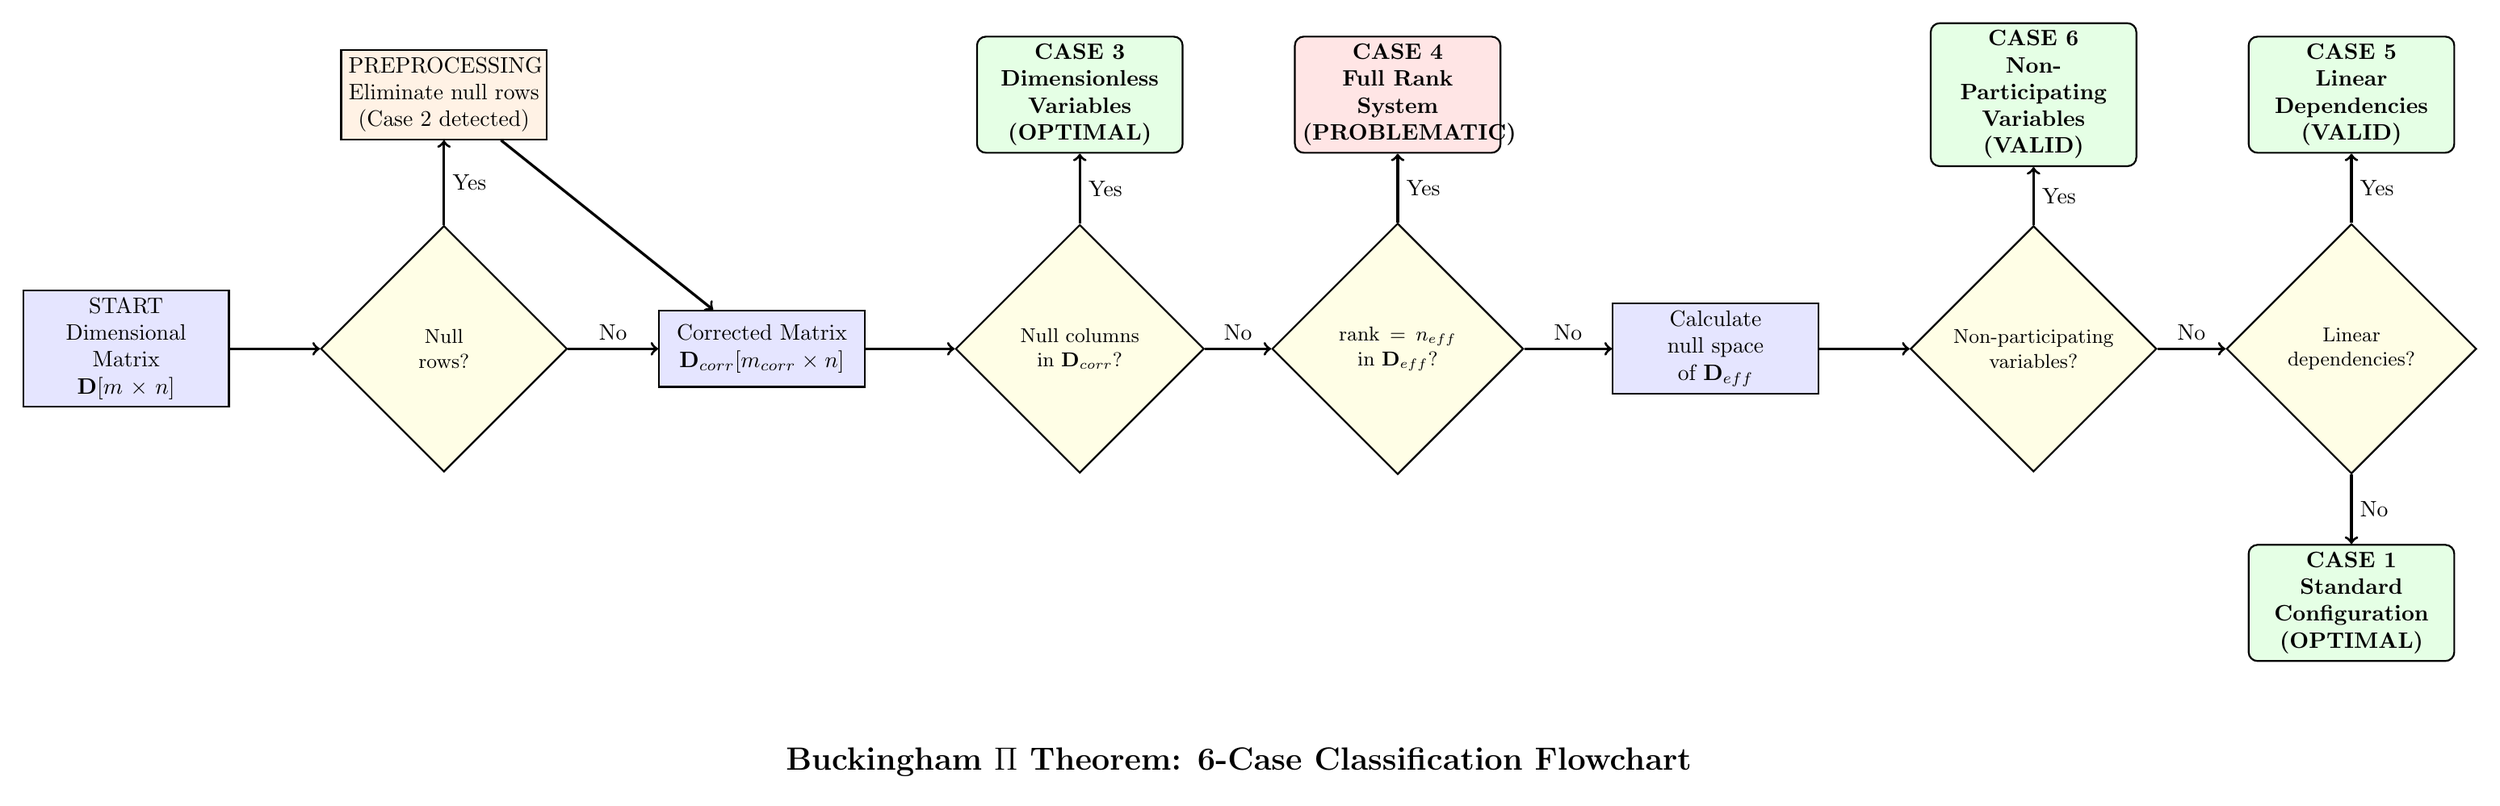
\begin{tikzpicture}[
    node distance=2cm and 4.5cm,
    box/.style={rectangle, draw, thick, fill=blue!10, text width=3cm, text centered, minimum height=1.2cm, font=\normalsize},
    decision/.style={diamond, draw, thick, fill=yellow!10, text width=2.8cm, text centered, minimum height=1.2cm, font=\small},
    case/.style={rectangle, rounded corners, draw, thick, fill=green!10, text width=3cm, text centered, minimum height=1.2cm, font=\normalsize\bfseries},
    problematic/.style={rectangle, rounded corners, draw, thick, fill=red!10, text width=3cm, text centered, minimum height=1.2cm, font=\normalsize\bfseries},
    preprocessing/.style={rectangle, draw, thick, fill=orange!10, text width=3cm, text centered, minimum height=1.2cm, font=\normalsize},
    arrow/.style={->, very thick}
]

% Main horizontal flow - all nodes in a single row with wider spacing
\node[box] (start) at (0,0) {START\\Dimensional Matrix\\$\mathbf{D}[m \times n]$};

\node[decision] (null_rows_check) at (5,0) {Null\\rows?};

\node[box] (corrected_matrix) at (10,0) {Corrected Matrix\\$\mathbf{D}_{corr}[m_{corr} \times n]$};

\node[decision] (null_cols) at (15,0) {Null columns\\in $\mathbf{D}_{corr}$?};

\node[decision] (full_rank) at (20,0) {$\text{rank} = n_{eff}$\\in $\mathbf{D}_{eff}$?};

\node[box] (null_space) at (25,0) {Calculate\\null space\\of $\mathbf{D}_{eff}$};

\node[decision] (non_participating) at (30,0) {Non-participating\\variables?};

\node[decision] (dependencies) at (35,0) {Linear\\dependencies?};

% Cases positioned above and below with greater separation
\node[preprocessing] (eliminate_rows) at (5,4) {PREPROCESSING\\Eliminate null rows\\(Case 2 detected)};

\node[case] (case3) at (15,4) {CASE 3\\Dimensionless\\Variables\\(OPTIMAL)};

\node[problematic] (case4) at (20,4) {CASE 4\\Full Rank\\System\\(PROBLEMATIC)};

\node[case] (case6) at (30,4) {CASE 6\\Non-Participating\\Variables\\(VALID)};

\node[case] (case5) at (35,4) {CASE 5\\Linear\\Dependencies\\(VALID)};

\node[case] (case1) at (35,-4) {CASE 1\\Standard\\Configuration\\(OPTIMAL)};

% Main horizontal flow arrows
\draw[arrow] (start) -- (null_rows_check);
\draw[arrow] (null_rows_check) -- node[above] {No} (corrected_matrix);
\draw[arrow] (corrected_matrix) -- (null_cols);
\draw[arrow] (null_cols) -- node[above] {No} (full_rank);
\draw[arrow] (full_rank) -- node[above] {No} (null_space);
\draw[arrow] (null_space) -- (non_participating);
\draw[arrow] (non_participating) -- node[above] {No} (dependencies);

% Vertical arrows to cases with better spacing
\draw[arrow] (null_rows_check) -- node[right] {Yes} (eliminate_rows);
\draw[arrow] (eliminate_rows) -- (corrected_matrix);

\draw[arrow] (null_cols) -- node[right] {Yes} (case3);

\draw[arrow] (full_rank) -- node[right] {Yes} (case4);

\draw[arrow] (non_participating) -- node[right] {Yes} (case6);

\draw[arrow] (dependencies) -- node[right] {Yes} (case5);
\draw[arrow] (dependencies) -- node[right] {No} (case1);

% Title positioned lower and more prominent
\node[font=\Large\bfseries, text centered] at (17.5,-6.5) {Buckingham $\Pi$ Theorem: 6-Case Classification Flowchart};

\end{tikzpicture}
}
\end{figure} 